\documentclass[a4paper]{book}
\usepackage[utf8]{inputenc}

\usepackage{geometry}
\usepackage{bookmark,hyperref}
\usepackage{xcolor}
\usepackage[english]{babel}
\usepackage{graphicx}


\usepackage{amsmath}
\usepackage{amsfonts}
\usepackage{amsthm}

\usepackage{mathrsfs}
\usepackage{bbm}
\usepackage{enumitem}
\usepackage{cleveref}
\usepackage{titlesec}
\usepackage{minitoc}
\usepackage{fancyhdr}
\usepackage{ragged2e}
\usepackage{algorithm}
\usepackage{algorithmic}

\usepackage{tikz}
\usetikzlibrary{arrows.meta}

\hypersetup{colorlinks, linkcolor=red, citecolor=blue, urlcolor=blue, bookmarksopen=true, bookmarksopenlevel=0}



% mathbb
\newcommand{\CC}{\mathbb{C}}
\newcommand{\EE}{\mathbb{E}}
\newcommand{\NN}{\mathbb{N}}
\newcommand{\PP}{\mathbb{P}}
\newcommand{\QQ}{\mathbb{Q}}
\newcommand{\RR}{\mathbb{R}}
\newcommand{\VV}{\mathbb{V}}

% mathcal
\newcommand{\cA}{\mathcal{A}}
\newcommand{\cB}{\mathcal{B}}
\newcommand{\cC}{\mathcal{C}}
\newcommand{\cD}{\mathcal{D}}
\newcommand{\cE}{\mathcal{E}}
\newcommand{\cF}{\mathcal{F}}
\newcommand{\cG}{\mathcal{G}}
\newcommand{\cH}{\mathcal{H}}
\newcommand{\cI}{\mathcal{I}}
\newcommand{\cJ}{\mathcal{J}}
\newcommand{\cK}{\mathcal{K}}
\newcommand{\cL}{\mathcal{L}}
\newcommand{\cM}{\mathcal{M}}
\newcommand{\cN}{\mathcal{N}}
\newcommand{\cO}{\mathcal{O}}
\newcommand{\cP}{\mathcal{P}}
\newcommand{\cQ}{\mathcal{Q}}
\newcommand{\cR}{\mathcal{R}}
\newcommand{\cS}{\mathcal{S}}
\newcommand{\cT}{\mathcal{T}}
\newcommand{\cV}{\mathcal{V}}
\newcommand{\cW}{\mathcal{W}}
\newcommand{\cX}{\mathcal{X}}
\newcommand{\cY}{\mathcal{Y}}
\newcommand{\cZ}{\mathcal{Z}}

% mathscr
\newcommand{\sA}{\mathscr{A}}
\newcommand{\sB}{\mathscr{B}}
\newcommand{\sI}{\mathscr{I}}
\newcommand{\sM}{\mathscr{M}}
\newcommand{\sO}{\mathscr{O}}
\newcommand{\sP}{\mathscr{P}}
\newcommand{\sR}{\mathscr{R}}
\newcommand{\sT}{\mathscr{T}}
\newcommand{\sX}{\mathscr{X}}
\newcommand{\sY}{\mathscr{Y}}
\newcommand{\sZ}{\mathscr{Z}}

% \theoremstyle{plain}
% \newtheorem{thm}{Theorem}[chapter]
% \crefname{thm}{theorem}{theorems}
% \newtheorem{prop}{Proposition}[chapter]
% \crefname{prop}{proposition}{propositions}
% \newtheorem{lem}{Lemma}[chapter]
% \crefname{lem}{lemma}{lemmas}
% \newtheorem{cor}{Corollary}[chapter]
% \crefname{cor}{corollary}{corollaries}

% \theoremstyle{definition}
% \newtheorem{defi}{Definition}[chapter]
% \crefname{defi}{definition}{definitions}
% \newtheorem{assu}{Assumption}[chapter]
% \crefname{assu}{assumption}{assumptions}
% \newtheorem{rem}{Remark}[chapter]
% \crefname{rem}{remark}{remarks}
% \newtheorem{ex}{Example}[chapter]
% \crefname{ex}{example}{examples}

% operateurs
\DeclareMathOperator{\Tr}{Tr}
\DeclareMathOperator{\Supp}{Supp}
\DeclareMathOperator{\Vect}{Vect}
\DeclareMathOperator*{\argmin}{arg\,min}
\DeclareMathOperator*{\argmax}{arg\,max}
\DeclareMathOperator{\Cov}{Cov}
\DeclareMathOperator{\Var}{Var}
\DeclareMathOperator{\erf}{erf}
\DeclareMathOperator*{\tend}{\to}
\newcommand{\rD}{\mathrm{D}}
\def\bX{\mathbf{X}}
\DeclareMathOperator{\diag}{diag}
\DeclareMathOperator{\Span}{Span}
\DeclareMathOperator{\Image}{im}
\DeclareMathOperator{\Kernel}{ker}


\newcommand{\conv}[2][\ ]{\overset{#1}{\underset{#2}{\to}}}
\newcommand{\aseq}[2][]{\overset{#1}{\underset{#2}{=}}}
\newcommand{\equi}[1]{\underset{#1}{\sim}}
\newcommand{\mbf}[1]{\mathbf{#1}}
\newcommand{\indic}{\mathbbm{1}}
\newcommand{\hatmbf}[1]{\hat{\mathbf{#1}}}
\let\eps\varepsilon
\let\to\longrightarrow


\newenvironment{abstract}[1][Abstract]{\paragraph{#1}}{}





% \defbibheading{none}{%
% }
% \DeclareSourcemap{
%   \maps[datatype=bibtex]{
%     \map[overwrite]{
%       \perdatasource{biblio.bib}
%       \step[fieldset=keywords, fieldvalue={,conf}, append]
%     }
%   }
% }




\newcommand{\PhDTitle}{%
	%Reference priors: objective and practical inference,applied for auditable estimations of seismic fragility curves\\%
    %
    Extended reference prior theory for objective and practical inference, application to %\makebox[4em][r]
    {robust and auditable seismic fragility curves%}
}}

\newcommand{\logoEd}{EDMH}																		%% Logo de l'école doctorale. Indiquer le sigle (EDIPP, EDMH) / Doctoral school logo. Indicate the acronym : EDMH, EDIPP
\newcommand{\PhDTitleFR}{Théory des priors de référence étendue pour une inférence objective et pratique, application pour des estimateurs auditable de courbes de fragilité sismique}													%% Titre de la thèse en français / Thesis title in french
\newcommand{\keywordsFR}{Prior objectif, Analyse bayésienne, Aléa sismique, Courbe de fragilité, Quantification des incertitudes}														%% Mots clés en français, séprarés par des , / Keywords in french, separated by ,
\newcommand{\abstractFR}{%
La théorie des priors de référence fournit un cadre approprié à une inférence bayésienne objective, puisqu'elle %visant à minimiser
vise à minimiser la subjectivité introduite et à permettre aux informations issues des données d'orienter la distribution des estimations. Pour cette raison, l'application de cette théorie à l'estimation des courbes de fragilité sismique est particulièrement pertinente. En effet, ces courbes
sont des éléments essentiels
des études simsmiques probabilistes de sûreté~; elles expriment la probabilité de défaillance d'une structure mécanique en fonction d'indateurs définissant des scénarios sismiques. Puisqu'elles informent des décisions critiques en matière de sécurité des infrastructures, une auditabilité complète de l'approche qui conduit aux estimations de ces courbes est nécessaire.

Cette thèse étudie l'interaction entre la théorie des priors de référence et l'estimation des courbes de fragilité sismique, apportant des contributions originales dans ces deux domaines. Tout d'abord, nous complétons les fondements théoriques des priors de référence en développant de nouvelles constructions de ceux-ci. Notre objectif est de soutenir leur objectivité tout en améliorant leur applicabilité pratique. Nos résultats prennent la forme de contributions théoriques dans ce domaine qui sont basées sur une définition généralisée de l'information mutuelle. Nos approches abordent les principaux problèmes des priors de référence, à savoir le caractère impropre de leur distribution ou de leu distribution \emph{a posteriori}, et leur formulation complexe pour une utilisation pratique.

Esnuite, nous revisitons l'estimation des courbes de fragilité sismique basée sur le modèle probit-lognormal dans un contexte où les données sont particulièrement rares. Notre objectif est de réaliser une estimation bayésienne des courbes de fragilité qui tire parti de l'optimisation de toutes sortes d'informations, y compris l'information \emph{a priori}, afin de fournir des estimations robustes et auditables. Nos résultats mettent en évidence les limites et les irrégularités du modèle et proposent des méthodes qui fournissent des estimations précises et efficaces des courbes. Les évaluations de nos approches sont réalisées sur différents cas d'étude issus de l'industrie nucléaire.

Cette thèse établit un lien fort entre ces deux domaines. L'application aux courbes de fragilité sismique a non seulement motivé les développements théoriques mais leur a aussi directement profité, produisant finalement un cadre d'estimation plus robuste, interprétable et vérifiable.
}															%% Résumé en français / abstract in french

\newcommand{\PhDTitleEN}{\PhDTitle}													%% Titre de la thèse en anglais / Thesis title in english
\newcommand{\keywordsEN}{Objective prior, Bayesian analysis, Seismic hazard, Fragility curve, Uncertainties quantification}														%% Mots clés en anglais, séprarés par des , / Keywords in english, separated by ,
\newcommand{\abstractEN}{%
Reference prior theory provides a principled framework for objective Bayesian inference, aiming to minimize subjective input and allow data-based information to drive the estimates distribution. %This is particularly valuable in high-stakes applications, where transparency, auditability, and robustness are essential. 
% This theory becomes particularly relevant for
For this reason, the application of this theory to the estimation of seismic fragility curves is particularly relevant.
Indeed, these curves are essential elements of seismic probabilistic risk assessment studies; they express the probability of failure of a mechanical structure as a function of indicators that define 
seismic scenarios. Since they inform critical decisions in infrastructure safety, a complete auditability of the pipeline that leads to the estimates of these curves is required.
% they require a total auditability and robustness of the pipeline that produce estimates of them.

%One such application is the estimation of seismic fragility curves—probabilistic tools that characterize structural failure likelihood as a function of earthquake intensity. These curves play a central role in seismic probabilistic risk assessment, where they inform critical decisions in infrastructure safety and resilience.

This thesis investigates the interplay between reference prior theory and seismic fragility curves estimation, yielding original contributions in these two domains. First, we complement the theoretical foundations of reference priors by developing novel constructions of them. 
Our goal is to support their objectivity while improving their practical applicability. Our results take the form of
theoretical contributions in this domain that are based on a generalized definition of the mutual information.
Our approaches tackle the principal issues of reference priors, namely their improper characteristic or that of their posterior, and their complex formulation for practical use.

%  definition of reference priors
% We tackle the pincipal issues encountered by using the referebce prios in practice by proposing methods that address 
% We provide adaptations of the reference priors definiton
% three theoretical contributions in this domain that propose (i)~an extension of the thoery that supports the objectivity of the Jeffreys prior, (ii)~constraints that can be incorporated to the prior to enhance.
%Our goal is to question the balance between obejctivity
%under constraints, improving their practical applicability, and proposing ways to evaluate and compare their objectivity. 
Second, we revisit the estimation of seismic fragility curves based on the prominent probit-lognormal model in a context where the data are particularly sparse.
Our goal is to conduct a Bayesian estimation of seismic fragility curves that leverages the optimization of every sort of information, including the \emph{a priori} one, in order to provide estimates that are robust and auditable.
Our results highlight the limitations and irregularities of the model and propose methods that provide accurate and efficient estimates of the curves. The evaluations of our approaches are carried out on different case studies taken from the nuclear industry.

%a common yet delicate setting due to data sparsity and binary observations. We formally compute the Jeffreys prior for this model, highlight its limitations, and introduce alternative priors that address issues of degeneracy and inefficiency. We also incorporate optimal experimental design to improve estimation quality.

This thesis builds a strong link between these two domains.
The application to seismic fragility curves not only motivated theoretical developments but also directly benefited them, ultimately producing a more robust, interpretable, and verifiable estimation framework.
%The application to seismic fragility curves not only motivates theoretical developments but also benefits directly from them, yielding estimation pipelines that are more robust, interpretable, and auditable. %Through this bi-directional dialogue, %, we demonstrate how abstract statistical theory can be meaningfully applied to real-world engineering problems.
%we illustrate how reference prior theory can be extended and applied to meet the needs of modern reliability analysis.
}

% \renewcommand{\abstractFR}{\abstractEN}



% The reference prior theory provides the means to define a prior that can be qualified as ``objective''.
% stands as a cornerstone of objective Bayesian analysis. By formally defining priors that aim to minimize the influence of subjective information, it offers a principled framework for drawing inferences that are driven primarily by the observed data. 
% For this reason, the framework of reference prior theory becomes significantly relevant for the estimation of seimsic fragilty curves. Indeed, these curves represent a central component of seismic probabilistic risk assessment studies as they quantify the probability of failure of a mechanical component under a specific seimic scenario. 

% The work developed in this thesis is threefold. First, we make original contributions to the theory of reference priors itself. While the theory has matured significantly since its inception, limitations remain—particularly in its capacity to yield practical and well-behaved priors in complex or constrained settings. We propose new ways to construct and interpret reference priors under conditional constraints, investigate their asymptotic properties, and develop diagnostic tools to compare competing priors in terms of objectivity and robustness. These developments both clarify and extend the mathematical foundations of the theory, paving the way for its application in real-world settings where priors must meet practical requirements.

% Second, we focus on the estimation of seismic fragility curves, specifically under the widely used probit-lognormal model. In this context, observations are typically binary (e.g., structure failed or survived), and data scarcity often undermines the stability of classical estimates. We revisit the estimation problem from a Bayesian perspective, beginning with the formal computation of the Jeffreys prior for this model. We show that, while theoretically objective, this prior exhibits limitations in practice—such as posterior degeneracy in low-information regimes. We respond with methodological innovations, including a new class of constrained reference priors that explicitly address these issues. Furthermore, we explore how experimental design can be integrated into the inferential process to optimally extract information from limited data, significantly improving the robustness and interpretability of fragility estimates.

% Third, and most critically, we bridge the gap between these two domains—using the application to seismic fragility curves as both a proving ground and a source of inspiration for the development of reference prior theory. This bi-directional interplay is a central theme of the thesis. On one hand, the challenges encountered in fragility modeling motivate theoretical advances in the construction and evaluation of priors. On the other, these advances enable new and more reliable methods for estimating fragility curves, especially in data-poor settings. For instance, we demonstrate how sensitivity to prior assumptions can be controlled and quantified within the reference prior framework, enhancing the explainability and auditability of the final risk estimates.

% Taken together, the results of this work not only advance the frontier of objective Bayesian analysis but also deliver tangible improvements to the practice of seismic risk assessment. The integration of these two threads—reference prior theory and fragility curve estimation—offers a powerful example of how abstract statistical ideas can be harnessed to meet concrete engineering needs.
% }															
%% Résumé en anglais / abstract in english




%% Membre n°1 (Président) / Member n°1 (President)
\newcommand{\jurynameA}{Nicolas Bousquet}
\newcommand{\juryadressA}{Professeur, Sorbonne université, LPSM}
\newcommand{\juryroleA}{Rapporteur}

%%% Membre n°2 (Rapporteur) / Member n°2 (Reviewer)
\newcommand{\jurynameB}{Daniel Straub}
\newcommand{\juryadressB}{Professeur, TU Munich, Engineering Risk Analysis Group}
\newcommand{\juryroleB}{Rapporteur}

%%% Membre n°3 (Rapporteur) / Member n°3 (Reviewer)
\newcommand{\jurynameC}{Sophie Ancelet}
\newcommand{\juryadressC}{Ingénieure de recherche, ASNR}
\newcommand{\juryroleC}{Examinatrice}

%%% Membre n°4 (Examinateur) / Member n°4 (Examiner)
\newcommand{\jurynameD}{Julyan Arbel}
\newcommand{\juryadressD}{Chargé de recherche, Inria Grenoble}
\newcommand{\juryroleD}{Examinateur}

%%% Membre n°5 (Directeur de thèse) / Member n°5 (Thesis supervisor)
\newcommand{\jurynameE}{Olivier Le Maître}
\newcommand{\juryadressE}{Directeur de recherche, École polytechnique, CMAP}
\newcommand{\juryroleE}{Examinateur}

\newcommand{\jurynameF}{Mathilde Mougeot}
\newcommand{\juryadressF}{Professeure, ENS Paris-Saclay, Centre Borelli}
\newcommand{\juryroleF}{Examinatrice}

%%% Membre n°6 (Co-directeur de thèse) / Member n°6 (Thesis co-supervisor)
\newcommand{\jurynameG}{Josselin Garnier}
\newcommand{\juryadressG}{Professeur, École polytechnique, CMAP}
\newcommand{\juryroleG}{Directeur de thèse}

%%% Membre n°7 (Invité) / Member n°7 (Guest)
\newcommand{\jurynameH}{Cyril Feau}
\newcommand{\juryadressH}{Ingénieur de recherche, CEA Saclay, SEMT}
\newcommand{\juryroleH}{Encadrant}

%% Membre n°8 (Invité) / Member n°8 (Guest)
\newcommand{\jurynameI}{Clément Gauchy}
\newcommand{\juryadressI}{Ingénieur de recherche, CEA Saclay, SGLS}
\newcommand{\juryroleI}{Invité}
% \usepackage[utf8]{inputenc}
\usepackage{helvet}
\renewcommand{\familydefault}{\sfdefault}
% \usepackage{geometry}
\geometry{
	left=20mm,
	top=30mm,
	right=20mm,
	bottom=30mm
}
% \usepackage{xcolor}
\usepackage[absolute,overlay]{textpos}
% \usepackage{graphicx}
\usepackage{lipsum}
\usepackage{array}
\usepackage{caption}
\usepackage{multicol}
\setlength{\columnseprule}{0pt}
\setlength\columnsep{10pt}
% \usepackage[english]{babel}
\usepackage{anyfontsize}
\usepackage{ifxetex}

 
\ifxetex
  \DeclareGraphicsRule{.ai}{QTm}{QTm}{#1}
\else
  \DeclareGraphicsRule{.ai}{pdf}{.ai}{}
\fi


\usepackage[backend=biber, style=authoryear, natbib=true, maxnames=4, maxcitenames=3, maxbibnames=5]{biblatex}
\addbibresource{biblio.bib}



\usepackage[osf]{mathpazo} %sc
\linespread{1.05} 

% full arabic numbering of the pages

% \makeatletter
% \renewcommand{\frontmatter}{\cleardoublepage\@mainmatterfalse}
% \renewcommand{\mainmatter}{\cleardoublepage\@mainmattertrue}
% \makeatother
% \usepackage[amsmath,thmmarks,framed]{ntheorem} 

\usepackage[style=0,ntheorem]{mdframed}
\mdfsetup{%
topline=false,
rightline=false,
bottomline=false,
linewidth=1.5pt,
innerleftmargin=10pt,
innerrightmargin=0pt,
skipabove=\baselineskip,
skipabove=1.2\baselineskip,
}

% \newtheorem{mdbeispiel}{Beispiel}[section]
% \newtheorem{mdspiele}{Spiele}[section]
% \newenvironment{beispiel}[1][]%
%    {\begin{mdframed}[linecolor=blue]\begin{mdbeispiel}[#1]}
%    {\end{mdbeispiel}\end{mdframed}}
% \newenvironment{spiele}[1][]%
%    {\begin{mdframed}[linecolor=red]\begin{mdspiele}[#1]}
%    {\end{mdspiele}\end{mdframed}}
% \newframedRtheorem{beispiel}{Beispiel}[section]
% \newframedBtheorem{theo}[beispiel]{Theorem}
% \newframedGtheorem{exam}[beispiel]{Example}
% \theoremstyle{plain}





\DeclareSymbolFont{CMletters}{OML}{cmm}{m}{it}
\DeclareMathSymbol{\xi}{\mathord}{CMletters}{"18}
\DeclareMathSymbol{j}{\mathalpha}{CMletters}{"6A}



\definecolor{niceBlue}{HTML}{023E8A}
\definecolor{niceBluelight}{HTML}{0077B6}
\definecolor{ayellow}{HTML}{D62828}
\hypersetup{linkcolor=niceBlue, citecolor=niceBlue, urlcolor=niceBlue}

\renewcommand{\beforeminitoc}{\vspace*{-12pt}}%\hypersetup{linkcolor=niceBluelight}}
% \renewcommand{\afterminitoc}{\hypersetup{linkcolor=niceBlue}}

\mtcsetrules{minitoc}{off}

\renewcommand{\mtctitle}{}

\usepackage{anyfontsize}
\titleformat{\chapter}[display]{\Huge\raggedleft}{\fontsize{40}{45}\selectfont\color{niceBlue}\thechapter}{0pt}{\vspace*{0.5em}}

% \titleformat*{\section}{\Large\color{niceBlue}}

\titleformat{\part}[block]{\color{niceBlue}\Huge\MakeUppercase\centering}{\begin{center}\fontsize{40}{45}\selectfont\Roman{part}\end{center}}{0pt}{\Huge\scshape}

% \titlelabel{\thepar}
% \titleformat*{\part}{\fontsize{30}{35}\selectfont\scshape\centering}


\renewenvironment{abstract}[1][Abstract]{\begin{center}\begin{minipage}{0.87\textwidth}\paragraph{\hspace*{2.5em}#1}}{\end{minipage}\end{center}}


\renewcommand{\chaptermark}[1]{%
\markboth{#1}{}}
\renewcommand{\sectionmark}[1]{\markright{#1}}


\fancyhead[EL]{\color{niceBlue}\chaptertitlename\ \thechapter.\ \emph{\leftmark}}
\fancyhead[ER]{}
\fancyhead[OR]{\color{niceBlue}\thesection.\ \emph{\rightmark}}
\fancyhead[OL]{}

\renewcommand{\headrulewidth}{0pt}


\crefformat{chapter}{\textcolor{niceBlue}{#2\MakeLowercase\chaptertitlename~#1#3}}
\Crefformat{chapter}{\textcolor{niceBlue}{#2\chaptertitlename~#1#3}}

\crefformat{part}{\textcolor{niceBlue}{#2\MakeLowercase\partname~#1#3}}
\Crefformat{part}{\textcolor{niceBlue}{#2\partname~#1#3}}




\newtheoremstyle{mythmstyle}{0pt}{2pt}{\itshape}{}{\bfseries}{.}{0.5em}{}
\theoremstyle{mythmstyle}

\newtheorem{fthm}{Theorem}[chapter]
\crefname{fthm}{theorem}{theorems}
\newtheorem{fprop}{Proposition}[chapter]
\crefname{fprop}{proposition}{propositions}
\newtheorem{flem}{Lemma}[chapter]
\crefname{flem}{lemma}{lemmas}
\newtheorem{fcor}{Corollary}[chapter]
\crefname{fcor}{corollary}{corollaries}

\newenvironment{thm}[1][]%
   {\begin{mdframed}[linecolor=niceBluelight]\begin{fthm}[#1]}
   {\end{fthm}\end{mdframed}}
\newenvironment{prop}[1][]%
   {\begin{mdframed}[linecolor=niceBluelight]\begin{fprop}[#1]}
   {\end{fprop}\end{mdframed}}
\newenvironment{lem}[1][]%
   {\begin{mdframed}[linecolor=niceBluelight]\begin{flem}[#1]}
   {\end{flem}\end{mdframed}}
\newenvironment{cor}[1][]%
   {\begin{mdframed}[linecolor=niceBluelight]\begin{fcor}[#1]}
   {\end{fcor}\end{mdframed}}

\theoremstyle{definition}
\newtheorem{fdefi}{Definition}[chapter]
\crefname{fdefi}{definition}{definitions}
\newenvironment{defi}[1][]%
   {\begin{mdframed}[linecolor=niceBluelight]\begin{fdefi}[#1]}
   {\end{fdefi}\end{mdframed}}

\newtheorem{assu}{Assumption}[chapter]
\crefname{assu}{assumption}{assumptions}
\newtheorem{rem}{Remark}[chapter]
\crefname{rem}{remark}{remarks}
\newtheorem{ex}{Example}[chapter]
\crefname{ex}{example}{examples}




\makeatletter
\renewenvironment{proof}[1][\proofname]{\begin{mdframed}[linecolor=gray]\par
\pushQED{\qed}%
\normalfont \topsep6\p@\@plus6\p@\relax
\trivlist
\item\relax
{\itshape
#1\@addpunct{.}}\hspace\labelsep\ignorespaces
}{%
\popQED\endtrivlist\@endpefalse
\end{mdframed}}
\makeatother


\title{\hrule\vspace*{0.5em}
    \textbf{Bayesian estimation of seismic fragility for industrial installations and structures}
    \vspace*{0.5em}\\ \hrule
    }
\author{Antoine Van Biesbroeck}

\date{DATE}
%
%\vfill
%\begin{center}
%    
%\end{center}


\setlength{\parskip}{0.25em}

\begin{document}
% \frontmatter
\pagestyle{empty}
%%%%%%%%%%%%%%%%%%%%%%%%%%%%%%%%%%%%%%%%%%%%%%%%%%%%%%%%%%%%%%%%%%%%%%%%%%%%%%%%%%%%%%%%%%%%%%%%%%%%%%%%%%%%%%%%%%%%%%%%%%%%%%%%%%%%%%%%%%%%%%%%%%%%%%%%%%%%%%%%%%%%%%%
%%%%%%%%%%%%%%%%%%%%%%%%%%%%%%%%%%%%%%%%%%%%%%%%%%%%%%%%%%%%%%%%%%%%%%%%%%%%%%%%%%%%%%%%%%%%%%%%%%%%%%%%%%%%%%%%%%%%%%%%%%%%%%%%%%%%%%%%%%%%%%%%%%%%%%%%%%%%%%%%%%%%%%%
%%% Modèle pour la 1ère de couverture des thèses préparées à l'Institut Polytechnique de Paris, basé sur le modèle produit par Guillaume BRIGOT / Template for front cover of thesis made at Institut Polytechnique de Paris, based on the template made by Guillaume BRIGOT
%%% Mis à jour par Aurélien ARNOUX (École polytechnique)/ Updated by Aurélien ARNOUX (École polytechnique)
%%% Les instructions concernant chaque donnée à remplir sont données en bloc de commentaire / Rules to fill this file are given in comment blocks
%%% ATTENTION Ces informations doivent tenir sur une seule page une fois compilées / WARNING These informations must contain in no more than one page once compiled
%%%%%%%%%%%%%%%%%%%%%%%%%%%%%%%%%%%%%%%%%%%%%%%%%%%%%%%%%%%%%%%%%%%%%%%%%%%%%%%%%%%%%%%%%%%%%%%%%%%%%%%%%%%%%%%%%%%%%%%%%%%%%%%%%%%%%%%%%%%%%%%%%%%%%%%%%%%%%%%%%%%%%%%
%%% Version du 25 mars 2019 : Ajout de détails dans les commentaires
%%%%%%%%%%%%%%%%%%%%%%%%%%%%%%%%%%%%%%%%%%%%%%%%%%%%%%%%%%%%%%%%%%%%%%%%%%%%%%%%%%%%%%%%%%%%%%%%%%%%%%%%%%%%%%%%%%%%%%%%%%%%%%%%%%%%%%%%%%%%%%%%%%%%%%%%%%%%%%%%%%%%%%%




\label{form}
%%%%%%%%%%%%%%%%%%%%%%%%%%%%%%%%%%%%%%%%%%%%%%%%%%%%%%%%%%%%%%%%%%%%%%%%%%%%%%%%%%%%%%%%%%%%%%%%%%%%%%%%%%%%%%%%%%%%%%%%%%%%%%%%%%%%%%%%%%%%%%%%%%%%%%%%%%%%%%%%%%%%%%%
%%%%%%%%%%%%%%%%%%%%%%%%%%%%%%%%%%%%%%%%%%%%%%%%%%%%%%%%%%%%%%%%%%%%%%%%%%%%%%%%%%%%%%%%%%%%%%%%%%%%%%%%%%%%%%%%%%%%%%%%%%%%%%%%%%%%%%%%%%%%%%%%%%%%%%%%%%%%%%%%%%%%%%%
%%% Formulaire / Form
%%% Remplacer les paramètres des \newcommand par les informations demandées / Replace \newcommand parameters by asked informations
%%%%%%%%%%%%%%%%%%%%%%%%%%%%%%%%%%%%%%%%%%%%%%%%%%%%%%%%%%%%%%%%%%%%%%%%%%%%%%%%%%%%%%%%%%%%%%%%%%%%%%%%%%%%%%%%%%%%%%%%%%%%%%%%%%%%%%%%%%%%%%%%%%%%%%%%%%%%%%%%%%%%%%%
%%%%%%%%%%%%%%%%%%%%%%%%%%%%%%%%%%%%%%%%%%%%%%%%%%%%%%%%%%%%%%%%%%%%%%%%%%%%%%%%%%%%%%%%%%%%%%%%%%%%%%%%%%%%%%%%%%%%%%%%%%%%%%%%%%%%%%%%%%%%%%%%%%%%%%%%%%%%%%%%%%%%%%%



% Development of the reference prior theory: 
% 	effiction and robust 
% 	Development of the efficient and robust reference priors
% 	prior theory for efficient
% 	Objectivity, practicability, and implementation of reference priors, objective Bayesian estimation of seimsic fragility curves
% Objectivism and practicability of the reference prirors, application to the estimation of seismic fragility curves
% Apprioate extension of the reference prior theory and objective Bayesian estimation of seimsic fragility curves
% } 	%% Titre de la thèse / Thesis title
\newcommand{\PhDname}{Antoine Van Biesbroeck} 															%% Civilité, nom et prénom /  Civility, first name and name 
\newcommand{\NNT}{20XXIPPAXXXX} 															%% Numéro National de Thèse (donnée par la bibliothèque à la suite du 1er dépôt)/ National Thesis Number (given by the Library after the first deposit)

\newcommand{\ecodoctitle}{École doctorale de mathématiques Hadamard} 													%% Nom de l'ED : École doctorale de l'Institut Polytechnique de Paris, École doctorale de mathématiques Hadamard  / Full name of Doctoral School : École doctorale de l'Institut Polytechnique de Paris, École doctorale de mathématiques Hadamard
\newcommand{\ecodocacro}{EDMH}																%% Sigle de l'ED : EDIPP, EDMH / Acronym of the Doctoral School : EDIPP, EDMH
\newcommand{\ecodocnum}{574} 																%% Numéro de l'école doctorale : 626 (EDIPP), 574 (EDMH) / Doctoral School number : 626 (EDIPP), 574 (EDMH)
\newcommand{\PhDspeciality}{Mathématiques appliquées} 										%% Spécialité de doctorat / Speciality 
\newcommand{\PhDworkingplace}{l'École polytechnique} 										%% Établissement de préparation / PhD working place :  l'École polytechnique, l'École nationale supérieure de techniques avancées, l'École nationale de la statistique et de l’administration économique, Télécom ParisTech, Télécom SudParis, l’École des hautes études commerciales de Paris   
\newcommand{\defenseplace}{Palaiseau} 											%% Ville de soutenance / Place of defense
\newcommand{\defensedate}{1er octobre 2025} 															%% Date de soutenance / Date of defense

%%% Établissement / Institution
%%% Si la thèse a été produite dans le cadre d'une co-tutelle, commenter la partie "Pas de co-tutelle" et décommenter la partie "Co-tutelle" / If the thesis has been prepared in guardianship, comment the part "Pas de co-tutelle" and uncomment the part "Co-tutelle"

	%%%%%%%%%%%%%%%%%%%%%%%%%
	%%% Pas de co-tutelle %%%
	%%%%%%%%%%%%%%%%%%%%%%%%%

%\newcommand{\logoEtt}{blank}																%% NE PAS MODIFIER / DO NOT MODIFY
\newcommand{\vpostt}{0.1} 																	%% NE PAS MODIFIER / DO NOT MODIFY
\newcommand{\hpostt}{6.1}																		%% NE PAS MODIFIER / DO NOT MODIFY
\newcommand{\logoEt}{media/etab/X-IPpairs-RVB.eps} 																	%% Logo de l'établissement de soutenance. Le nom du fichier correspond au sigle de l'établissement : ENSAE, ENSTA, TP, TSP, X  / Institution logo. Filename correspond to institution acronym : ENSAE, ENSTA, HEC, TP, TSP, X 
\newcommand{\vpos}{0.15}																		%% À modifier au besoin pour aligner le logo verticalement / If needed, modify to align logo vertilcally
\newcommand{\hpos}{13.25}																		%% À modifier au besoin pour aligner le logo horizontalement / If needed, modify to align logo horizontaly

		%%%%%%%%%%%%%%%%%%
		%%% Co-tutelle %%%
		%%%%%%%%%%%%%%%%%%

%\newcommand{\logoEt}{blank} 																%% Logo de l'université partenaire. Placer le fichier .png dans le répertoire '/media/etab' et indiquer le nom du fichier sans l'extension / Logo of partner university. Place the .png file in the directory '/media/etab' and point the file name without the extension
%\newcommand{\vpos}{0.1}																	%% À modifier au besoin pour aligner les logos verticalement / If needed, modify to align logos vertilcally
%\newcommand{\hpos}{12.25}																		%% À modifier au besoin pour aligner les logos horizontalement / If needed, modify to align logos horizontaly
%\newcommand{\logoEtt}{X}  																%% Logo de l'établissement de soutenance. Le nom du fichier correspond au sigle de l'établissement : ENSAE, ENSTA, TP, TSP, X  / Institution logo. Filename correspond to institution acronym : ENSAE, ENSTA, TP, TSP, X
%\newcommand{\vpostt}{0.1} 																	%% À modifier au besoin pour aligner les logos verticalement / If needed, modify to align logos vertilcally
%\newcommand{\hpostt}{6.1}																	%% À modifier au besoin pour aligner les logos horizontalement / If needed, modify to align logos horizontaly


%%% JURY

% Lors du premier dépôt de la thèse le nom du président n'est pas connu, le choix du président se fait par les membres du Jury juste avant la soutenance. La précision est apportée sur la couverture lors du second dépôt / Choice of the jury's president is made during the defense. Thus, it must be specified only for the second file deposition in ADUM.
% Tous les membres du juty listés doivent avoir été présents lors de la soutenance / All the jury members listed here must have been present during the defense.

%%% Membre n°1 (Président) / Member n°1 (President)
\newcommand{\jurynameA}{Nicolas Bousquet}
\newcommand{\juryadressA}{Professeur, Sorbonne université, LPSM}
\newcommand{\juryroleA}{Rapporteur}

%%% Membre n°2 (Rapporteur) / Member n°2 (Reviewer)
\newcommand{\jurynameB}{Daniel Straub}
\newcommand{\juryadressB}{Professeur, TU Munich, Engineering Risk Analysis Group}
\newcommand{\juryroleB}{Rapporteur}

%%% Membre n°3 (Rapporteur) / Member n°3 (Reviewer)
\newcommand{\jurynameC}{Sophie Ancelet}
\newcommand{\juryadressC}{Ingénieure de recherche, ASNR}
\newcommand{\juryroleC}{Examinatrice}

%%% Membre n°4 (Examinateur) / Member n°4 (Examiner)
\newcommand{\jurynameD}{Julyan Arbel}
\newcommand{\juryadressD}{Chargé de recherche, Inria Grenoble}
\newcommand{\juryroleD}{Examinateur}

%%% Membre n°5 (Directeur de thèse) / Member n°5 (Thesis supervisor)
\newcommand{\jurynameE}{Olivier Le Maître}
\newcommand{\juryadressE}{Directeur de recherche, École polytechnique, CMAP}
\newcommand{\juryroleE}{Examinateur}

\newcommand{\jurynameF}{Mathilde Mougeot}
\newcommand{\juryadressF}{Professeure, ENS Paris-Saclay, Centre Borelli}
\newcommand{\juryroleF}{Examinatrice}

%%% Membre n°6 (Co-directeur de thèse) / Member n°6 (Thesis co-supervisor)
\newcommand{\jurynameG}{Josselin Garnier}
\newcommand{\juryadressG}{Professeur, École polytechnique, CMAP}
\newcommand{\juryroleG}{Directeur de thèse}

%%% Membre n°7 (Invité) / Member n°7 (Guest)
\newcommand{\jurynameH}{Cyril Feau}
\newcommand{\juryadressH}{Ingénieur de recherche, CEA Saclay, SEMT}
\newcommand{\juryroleH}{Encadrant}

%% Membre n°8 (Invité) / Member n°8 (Guest)
\newcommand{\jurynameI}{Clément Gauchy}
\newcommand{\juryadressI}{Ingénieur de recherche, CEA Saclay, SGLS}
\newcommand{\juryroleI}{Invité}

%% Il est possible d'ajouter des membres supplémentaires selon le même modèle / More jury members can be added according to the same model

\label{layout}
%%%%%%%%%%%%%%%%%%%%%%%%%%%%%%%%%%%%%%%%%%%%%%%%%%%%%%%%%%%%%%%%%%%%%%%%%%%%%%%%%%%%%%%%%%%%%%%%%%%%%%%%%%%%%%%%%%%%%%%%%%%%%%%%%%%%%%%%%%%%%%%%%%%%%%%%%%%%%%%%%%%%%%%
%%%%%%%%%%%%%%%%%%%%%%%%%%%%%%%%%%%%%%%%%%%%%%%%%%%%%%%%%%%%%%%%%%%%%%%%%%%%%%%%%%%%%%%%%%%%%%%%%%%%%%%%%%%%%%%%%%%%%%%%%%%%%%%%%%%%%%%%%%%%%%%%%%%%%%%%%%%%%%%%%%%%%%%
%%% Mise en page / Page layout      
%%% NE RIEN MODIFIER EXCEPTÉ LA PARTIE CONCERNANT LE JURY (voir \label{jury}) SI BESOIN / DO NOT MODIFY EXCEPT SECTION CONCERNING JURY (see \label{jury}) IF NEEDED
%%%%%%%%%%%%%%%%%%%%%%%%%%%%%%%%%%%%%%%%%%%%%%%%%%%%%%%%%%%%%%%%%%%%%%%%%%%%%%%%%%%%%%%%%%%%%%%%%%%%%%%%%%%%%%%%%%%%%%%%%%%%%%%%%%%%%%%%%%%%%%%%%%%%%%%%%%%%%%%%%%%%%%%
%%%%%%%%%%%%%%%%%%%%%%%%%%%%%%%%%%%%%%%%%%%%%%%%%%%%%%%%%%%%%%%%%%%%%%%%%%%%%%%%%%%%%%%%%%%%%%%%%%%%%%%%%%%%%%%%%%%%%%%%%%%%%%%%%%%%%%%%%%%%%%%%%%%%%%%%%%%%%%%%%%%%%%%

% Méta-données du PDF / PDF meta-datas
\hypersetup{
	pdfauthor={\PhDname},
	pdfsubject={Manuscrit de thèse de doctorat},
	pdftitle={\PhDTitle},
}




\thispagestyle{empty}

\color{black} \hfill \vfill \tiny \ecodocnum
\begin{textblock}{5}(0,0)
	\textblockcolour{black}
	%\vspace{10mm}
	
\includegraphics [scale=0.95]{media/bandetransp2.png}
	\vspace{300mm}
\end{textblock}


\begin{textblock}{1}(0.6,3)
    \textblockcolour{} 
	\Large{\rotatebox{90}{\color{white}{\textbf{NNT : \NNT}}}}
\end{textblock}

\begin{textblock}{1}(0.85,8)
    \textblockcolour{} 
	\rotatebox{90}{\color{white}{{\fontsize{44}{60}\selectfont Thèse de doctorat}}}
\end{textblock}


                            

% \begin{textblock}{1}(\hpostt,\vpostt)
% 	\textblockcolour{white}
% 	\includegraphics[scale=1]{media/etab/\logoEtt.png} 
% \end{textblock}

\begin{textblock}{1}(\hpos,\vpos)
	\textblockcolour{white}
	
\includegraphics[width=2.64cm]{media/etab/X-IPparis-RVB.ai}
\end{textblock}

%\vspace{6cm}
%% Texte
\begin{textblock}{10}(5.7,3)
	\textblockcolour{white}
	
	\color{black}
	%\begin{center}  
	\begin{flushright}
		%\huge{
			\fontsize{19}{23}\selectfont\PhDTitle
			%}% 
			\\ \bigskip %% Titre de la thèse 
		\vfill
		\color{black} %% Couleur noire du reste du texte
		\normalsize {Thèse de doctorat de l'Institut Polytechnique de Paris} \\
		préparée à \PhDworkingplace \\ \bigskip
		\vfill
		École doctorale n$^{\circ}$\ecodocnum ~\ecodoctitle ~(\ecodocacro)  \\
		
		\small{Spécialité de doctorat: \PhDspeciality} \\ \bigskip %% Spécialité 
		\vfill  
		\footnotesize{Thèse présentée et soutenue à \defenseplace, le \defensedate, par} \\ \bigskip
		\vfill
		\Large{\textbf{\textsc{\PhDname}}} %% Nom du docteur
		\vfill
		%\bigskip
	\end{flushright}
	
	%\end{center}
	\color{black}
	%% Jury
	\begin{flushleft}
		
		\small Composition du Jury :
	\end{flushleft}
	%% Members of the jury

	\small
	%\begin{center}
	\newcolumntype{L}[1]{>{\raggedright\let\newline\\\arraybackslash\hspace{0pt}}m{#1}}
	\newcolumntype{R}[1]{>{\raggedleft\let\newline\\\arraybackslash\hspace{0pt}}lm{#1}}
	
	\label{jury} 																				%% Mettre à jour si des membres ont été ajoutés ou retirés / Update if members have been added or removed
	\begin{flushleft}
	\begin{tabular}{@{} L{9.64cm} R{4.5cm}}
		\jurynameA  \\ \juryadressA & \juryroleA \\[5pt]
		\jurynameB  \\ \juryadressB & \juryroleB \\[5pt]
		\jurynameC  \\ \juryadressC & \juryroleC \\[5pt]
		\jurynameD  \\ \juryadressD & \juryroleD \\[5pt]
		\jurynameE  \\ \juryadressE & \juryroleE \\[5pt]
		\jurynameF  \\ \juryadressF & \juryroleF \\[5pt]
		\jurynameG  \\ \juryadressG & \juryroleG \\[5pt]
		\jurynameH  \\ \juryadressH & \juryroleH \\[5pt]
		\jurynameI  \\ \juryadressI & \juryroleI \\[5pt]
	\end{tabular} 
	\end{flushleft}   
	%\end{center}
\end{textblock}


tests

\newpage 
\normalsize
\renewcommand{\familydefault}{\rmdefault}
\normalfont


\maketitle

%tests
%\newpage
\ 
\vfill
\begin{FlushRight}\itshape
A Pop\\
et Maminette
\end{FlushRight}
\vfill
Heureux sont les coeurs purs, car ils verront Dieu.

\newpage
% \mainmatter
\pagestyle{plain}

\chapter*{Remerciements}

% Je souhaite remercier en prime abord, mon bebou, qui a toujours été là pour moi (même si elle rechigne à lire mes articles de thèse). Je t'aime fort. 

\newpage

\chapter*{Abstract}

\chapter*{Résumé}


\dominitoc
\setcounter{tocdepth}{1}
\tableofcontents
\newpage
%\section{}

\pagestyle{fancy}\thispagestyle{plain}



\newlength{\questlenght}
\settowidth{\questlenght}{\textbf{Question iii}\ \ }
\newlength{\textminusquest}
\setlength{\textminusquest}{\textwidth}
\addtolength{\textminusquest}{-\questlenght}
\newcommand{\ques}[2]{%
\noindent\textbf{Question #1}\hfill
\begin{minipage}[t][25pt][t]{\textminusquest}
    #2
\end{minipage}    
}


\chapter{Introduction}\label{chap:intro-english}


\begin{abstract}
abstract
\end{abstract}

\minitoc


\section{Motivation and positioning of the thesis}






\subsection{Probabilistic risk assessment studies}



\subsection{Uncertainty quantification in probabilistic risk assessment studies}



\subsection{The choice of the prior in Bayesian studies}

\subsection{Motivating prior elicitation research for SPRA studies}



\section{Outline of the manuscript and contributions}

\subsection{Problems statement and organization of the thesis}



\subsection{List of contributions}













\chapter{Introduction en français}\label{chap:intro-french}

\renewcommand{\chaptername}{Chapitre}
\renewcommand{\partname}{Partie}


\begin{abstract}[Résumé]
    Ce chapitre ne diffère du \hyperref[chap:intro-english]{chapitre 1} que par sa rédaction en langue française.
    Dans ce chapitre, nous introduisons et motivons les travaux de recherche qui ont été conduits au court de cette thèse. Les travaux sont motivés
    principalement par le besoin d'évolution des méthodes d'études sismiques probabilistes de sûreté, mais aussi par le manque de réponse qu'apporte l'état-de-l'art à la question du choix du prior en inférence bayésienne.
    Ces problématiques sont détaillées et
    les travaux sont alors introduits comme s'inscrivant dans celles-ci, le tout donnant lieu à une organisation consistante du manuscrit.
    %en introduisant à la fois leur inscription dans le cadre des études sismiques probabilistes de sûreté et dans le
    %
    %D'une part, nous introduisons le cadre des études sismiques probabilistes de dûreté, et 
    % Dans ce chapitre, nous mettons en lumière les différentes problématiques, à la fois issue de qui motivent 
    % Dans ce chapitre, nous introduisons les différents contextes qui motivent l'existence de cette thèse. D
\end{abstract}

\minitoc

\section{Motivation et positionnement de la thèse}

\subsection{Etudes probabilistes de sûreté}
%

\subsubsection{Historique}

Les études probabilistes de sûreté (EPS) désignent un ensemble de méthodes d'analyses techniques qui permettent de quantifier un risque encouru par une installation lorsqu'elle est sujette à un évènement. L'évènement peut être d'origine naturelle comme artificielle, il peut être de provenance interne comme externe ; il peut s'agir d'un séisme, d'une inondation, d'une combinaison de défaillances internes, entre autres.  % (qui peut être d'origine naturelle comme artificielle, qui peut être interne comme externe). 

Faisant suite au premières recommandations de F. R. Farmer (expert sûreté à la UK atomic authority) dans les années 1960 pour la fiabilité des installations nucléaires,
ces méthodes ont pour caractéristique commune l'introduction de la notion d'incertitude dans la qualification de l'évènement, ses phénomènes et ses caractéristiques (on parle alors d'aléa).
%
%Elles ont été introduites par F. R. Farmer dans les années 1960 [], qui plébiscitait cette idée d'étudier la fiabilité des installations nucléaires en prenant en compte l'aspect probabiliste et incertain des évenements auqelles elle est sujette.
%
Leur cadre et leur concept ont été rapidement adoptés et développés aux Etats-Unis (cf. le rapport de la Nuclear Regulatory Commission, \cite{nrc_pra_1983}). En particulier, de nombreuses études sont venues dès 1968 (\cite{cornell_engineering_1968}) 
y inscrire les analyses de fiabilité parasismique, définissant alors le cadre des études sismiques probabilistes de sûreté (SPRA en anglais). %, en particulier en ce qui concerne le cadre de la fiabilité parasismque.



Le séisme représente en effet un facteur de risque remarquable des études de sûreté.
Premièrement, bien que communément caractérisé par sa magnitude et sa distance à la source, son signal est bien plus riche qu'une fonction bivariée et deux séismes de même magnitude et de même source peuvent avoir des caractéristiques (et des conséquences) significativement différentes.
Deuxièmement, puisqu'il touche à la fois tous les éléments aussi bien externes qu'internes à l'installation, il est la potentielle source de conséquences lourdes sur les équipements et structures.
%voir de réactions en chaîne 
%qui atteindraient le ``noyau dur'' de l'installation (défini comme un ensemble d'élements critiques à l'installation). %, impliquant ainsi un coût élevé.
Le coût potentiel des conséquences d'un aléa sismique peut alors être élevé et critique dans le contexte nucléaire, ce qui en fait un évènement d'intérêt majeur et décisif même dans les zones géographiques où il est rare.


%La prise en compte du séisme comme un aléa s'est confronté à la

Aujourd'hui, la prise en compte de l'aléa sismique sous le cadre des études probabilistes de sûreté est une recommandation internationale dans le contexte de l'industrie nucléaire. Leur cadre d'application dans l'industrie nucléaire française est précisé par l'autorité de sûreté nucléaire et de radioprotection (ASNR)\footnote{Anciennement ASN: l'autorité de sûreté nucléaire (ASN), a été unifiée avec l'institut de radioprotection et de sûreté nucléaire (IRSN) le 1\textsuperscript{er} janvier 2025.} dans la règle fondamentale de sûreté (\cite{asn_regle_2002}).









\subsubsection{L'évolution des EPS en France, au CEA, et dans cette thèse}



%Le rôle des études de sûreté d'une manière générale est de produire une quantification du risque d'une installation, d'une marge de fiabilité, et de démontrer son repsect d'un seuil défini par une autorité de régulation.
% Deux visions s'oppose relativement au sujet de l'avolution des méthodes et des conaissances relatives aux études de sûreté.
%Lors de la mise en place de de seuil et de la règle, plusieur point de vue, motivés par plusieurs intérêts peuvent alors se heurter. Il y a d'une part les exploitants, pour qui la notion de robustesse perdure d'elle même, les marges prises sont là pour tenir compte du manque de conaissances, et il y a ceux pour lesquels la robustess est sans cesse remise en question par les avancées des méthodes et des connaissances (\cite{roger_seisme_2020}).



%L'évolutions des méthodes et des conaissances relatives à la sûreté de 
L'évolution des méthodes et des connaissances relatives à la sûreté des installations nucléaires se fait de manière parallèle à l'évolution de la règle et de la norme imposées à celles-ci. 
Sur le sujet de l'aléa sismique, le rapport à l'évolution de la règle et de la méthode (et donc des EPS) oppose différents points de vue, principalement entre le principal exploitant (EDF) et les experts de l'autorité de sûreté (anciennement l'IRSN, maintenant unifié avec l'autorité de sûreté nucléaire devenue l'ASNR). 
Pour le premier, la robustesse de l'installation n'est normalement pas remise en question par l'avancée des connaissances et des méthodes puisque l’incertitude sur celles-ci fait parti des marges prises en comptes à la construction de l'équipement et calculées pour. Le second pense au contraire que la robustesse est une question perpétuelle et que la marge n’est pas pas faite pour être mordue au fil des connaissances qui s’ajoutent (\cite{roger_seisme_2020}). 
% L'évolution des méthodes EPS reste un champ de voies ouverte, pour lequel les approches s'opposent fondamentalement.
%Il est complxe de définir une voie d'évolution des EPS, et il n'y a pas de vision qui fait l'unanimté
L'ASNR se place alors en arbitre dans ce dialogue, entre autre elle définit le ``séisme majoré de sécurité''\footnote{Aujourd'hui plutôt appelé ``séisme noyau dur''.} (il s'agit d'une majoration du spectre du ``séisme maximal historiquement vraisemblable''\footnote{Aujourd'hui plutôt appelé ``séisme de dimensionnement''.}) qui sert de marge de référence dans la démonstration de robustesse parasismique d'un équipement. % la marge de fiablité et séisme maximal à prendre en compte. %En ce qui concerne l'aléa sismique, le dialogue 
%
%Un tel dialogue n'est pas propre à la France, et 


Cet arbitrage est donc à la fois sensible et critique.
L'incident survenu en 2011 à la centrale nucléaire de Fukushima-Daiichi le démontre. L'aléa sismique (qui est la cause du tsunami) de référence
%fixé par le concensus des experts japonais
a été sous-évalué par le consensus des experts japonais, et c'est cette sous-évaluation qui est au final la cause de l'incident (cf. le rapport de l'agence internationale de l'énergie atomique, \cite{iaea_fukushima_2015}).
%En 2011, a eu lieu un incident 
Suite à cet évènement, l'ASNR a pris la décision de majorer d'un facteur 1.5 le séisme majoré de sécurité en France, imposant une démonstration amplifiée de la robustesse des différentes installations par leur exploitant.



%En 2011, à la suite de l'incident à la centrale de Fukushima suite au séisme survenu au large des côtes japonaises, ce dialogue s'est conclut par une imposition de la part de l'autorité de sûreté d'une majoration d'un facteur de 1.5 de ce séisme majoré de sécurité en France. % de la marge de fiabilité sismique des équipements nucléaires en France. 

%Devant le coût induit par 

%Cette différence démontre de la complexité du sujet






% Le séisme ne fait pas exception
% la place des EPS simsique dans cette différence de vision est très marquée puisque l'aléa du séisme reste une quesiton ouverte en soi, la moindre différence de choix de séisme maximim possible peut donner lieu à une ampleur de changement d'un coût très élevé pour l'exploitant



%Les études probabilistes de sureté ont été adoptées progressivement en France 


%En France, l'industrie nucléaire est réduite à un nombre restreint d'acteurs, exploitants, experts indépendants, et autorité.

% Ambivalence de la robustesse, deux notions 
% deux visions
% Le CEA, à la fois exploitatn et expert

La place du CEA est ambivalente dans l'échiquier nucléaire français.
D'une part, il est exploitant d'installations nucléaires de recherche 
et joue alors son propre rôle quant à la démonstration de robustesse de ses équipements.
Aussi,
%, et ausi %titulaire d'une mission d'expertise de sûreté.
il participe à l'expertise conjointe des expertises de sûreté relatives au parc nucléaire civil exploité par EDF. 
%Le CEA joue son propre rôle dans l'évolution de la démonstration de la robustesse de ses propres equipements et installations. 
La recherche et l'expertise sur les causes de l'aléa sismique % études simqiques de sûreté au CEA 
se fait au CEA au laboratoire EMSI, qui dispose d'une plateforme expérimentale (Tamaris) qui permet de procéder à divers tests mécaniques sur des équipements sous séismes. 
%Le laboratoire d'etudes mécaniques et sismiques (EMSI) s'inscrit pleinenemnt dans cette ambivalence. Propriétaire de la plateforme d'expérimentation sismique Tamaris, le labortoire se place souvent au centre des études de fiabilité sismique et du dialogue entre EDF et les experts de l'ASNR.
L'approfondissement des méthodes des études sismiques probabilistes de sûreté est un enjeu du CEA qui s'inscrit dans ce laboratoire. Le CEA étant responsable devant les autorités de sûreté de ses installations, il cherche %alors 
à développer des méthodes toujours rigoureuses devant leur vieillissement. %de ces installations et de leurs équipements.



% Le rôle du CEA est ambivalent dans cete equation, à la fois exploitant instut de recherche.
% Le CEA joue son propre rôle dans l'évolutions de la démonstration de robstesse de ses propres installations. Aussi il participe à l'expertise conjointe de méthodes d'EPS avec EDF.


% Le CEA est lui même exploitant, d'unstallations de recherche.
% Il a 

% L'evolutio des EPS y est toujours un enjeux pour être capable de produire une étude plus efficace, et des résultats plus convaincants aurpès des autorités.
% Le CEA est responsable auprès des autorités concernant ses installations et cherche à développer des méthodes toujours rigoureuses devant le vieillissemnt des installations

% Sur le sujet de l'aléa sismique, la démonstration de robustesse reste complexe vis à vis de la complexité de l'aléa lui-même, et de sa fréquence.
% Les EPS sont en constantes ré-évaluation à la demande des autorités de sûreté sur cette aspect, principalement depuis l'accident sur la centrale de Fukushima en 2011. %%% Peut etre mettre ca plus haut

% Au CEA, la recherche sur les études sismiques probabilistes de sûerté est portée par le laboratoire EMSI, qui dispose d'une plateforme experimentale (Tamaris) qui permet de procéeder à divers tests mécaniques sur des équipements sous séismes. 

Cette thèse s'inscrit dans la démarche d'évolution du SPRA et de démonstration de sûreté. Financée par le CEA dans le cadre d'un contrat de formation par la recherche, elle a pour objectif d'étoffer l'état de l'art en terme d'estimation de fragilité sismique des équipements et des installations.
L'objectif est de développer des méthodes qui doivent le plus possible être (i) efficaces devant la complexité des objets étudiés et de la définition de l'aléa, (ii) être robustes dans le temps et devant une potentielle réévaluation des critères de sûreté, et (iii) être transparentes et auditables par les autorités de sûreté.

%lieu à des méthodes qui savent être efficace devant la complexité technique représentée efficaces devant la c

%en cherchant un cadre plus robuste, plus efficace.
%%%% Principalement en appuyant l'étude bayésienne de celles-ci.




\subsection{La quantification d'incertitudes dans les études probabilistes de sûreté} % la quantification d'incertitutde dans les EPS


\subsubsection{Principe et étapes de la quantification d'incertitudes}

%Le cadre des EPS regroupe un certains nmb
%Différents outils mathématiques sont employés dans le cadre des EPS et composent

Les études probabilistes de sûreté %et plus généralement les études probabilistes de fiabilité, de robustesse, et de  %les procédés de génie probabiliste d'études de fiabilité, de robustesse, et de 
s'appuient sur la 
prise en compte et la quantification des incertitudes qui apparaissent dans le procédé d'évaluation d'un risque au sein d'un système physique.
%lors de l'évaluation d'une quantité décrivant un risque. %d'un 
%
La quantification d'incertitudes représente en fait une démarche qui consiste à modéliser et analyser méthodiquement l'incertitude, sa source, et sa propagation au sein de la modélisation du système physique étudié. %étudié. %système phyisique?
Elle se construit alors à l'intersection de la physique, de l'ingénierie et des mathématiques appliquées, et s'érige même comme une branche des statistiques à part entière.

Elle concentre son étude sur 3 éléments qui décrivent l'interaction entre le système physique et l'aléa : des paramètres d'entrée $\mbf X$, une réponse physique du système $ Y$, et une modélisation de celle-ci selon : $ Y=\cM(\mbf X)$. % ($\cM$ peut-être définit comme la ).
Cette fonction $\cM$ est liée à la modélisation, souvent complexe, du système et de ses propriétés physiques (il peut s'agir de la résolution d'équations physiques, de simulation numériques, ou même du résultat d'une expérience mécanique).
%L'objet de la quantification d'incertitude est alors d'évaluer une quantité d'intérêt qui dépend de $\mbf Y$ : comme une variance, une probabilité de défaillance, etc ; plus généralement une quantité de la forme $\EE\,\phi(\mbf Y)$.
%
La démarche générale de la quantification d'incertitudes est souvent décrite au travers de différentes étapes clés (voir par ex. \cite{sudret_uncertainty_2007, iooss_contributions_2009}), à savoir : %au sein desquelles on distingue particulièrement l'étape d'identification des sources d'incertitudes.
%qu'on peutt principalement résumé 
%
\begin{enumerate}
    \item L'identification des sources incertitudes : 
        il est usuel de classifier les incertitudes selon deux grandes catégories. D'une part les incertitudes irréductibles, qui proviennent du hasard ``naturel'' embarqué dans l'aléa et le système physique. D'autre part, les incertitudes épistémiques, qui existent par manque d'information, et qui sont alors considérées comme réductibles en opposition aux précédentes (\cite{hullermeier_aleatoric_2019}). Il s'en suit une modélisation probabiliste de l'entrée $\mbf X$. 
    \item La propagation des incertitudes : cette étape correspondant à l'approximation de la distribution du modèle $\cM(\mbf X)$, et de l'évaluation d'une quantité d'intérêt qui dépend de celle-ci : comme une variance, une probabilité de défaillance, etc ; plus généralement une quantité de la forme $\EE\,\phi( Y)$.
%     et de celle de la quantité d'intérêt $\phi(\mbf Y)$. %De nombreuses méthodes mathématiques viennent en appui à cette étape, et sont évoquées plus bas.
    \item L'analyse de sensibilité : son rôle est de comprendre avec plus de recul la manière dont l'incertitude se propage dans un système, en identifiant l'impact d'un ou de plusieurs des paramètres d'entrées sur la sortie $ Y$ (\cite{iooss_review_2015}).
    %L'analyse de sensibilité se construit depuis les premier travaux de Sobol' (\cite{sobol_sensitivity_1993})
    %, lorsque les entrées sont multivariées ($X=(X_1,\dots,X_p)$), quelles sont celles  
\end{enumerate}


\subsubsection{Des outils mathématiques en quantification d'incertitudes}

%L'étape 1 sus-mentionnée s'ajoute à la modélisation du  modélisation
%Les étapes 2 et 3 ci-dessus mentionnées 
De nombreux outils mathématiques viennent appuyer les étapes sus-mentionnées. Bien que ce manuscrit n'a pas pour but d'en décrire un panel exhaustif, ci-dessous sont listés quelques exemples qui reviennent dans les travaux de cette thèse.
%en voici quelques uns qui sont omniprésents dans le domaine

\begin{itemize}
    \item La métamodélisation %, %le plus souvent par processus gaussien (appellé aussi krigeage), ou par polynomes du chaos, 
    permet de contrevenir la complexité d'évaluation du modèle $\cM$, en construisant un méta-modèle $\tilde\cM$, entraîné à partir d'une base de données d'observations $(\mbf x_1, y_1),\dots,(\mbf x_k,y_k)$. Le méta-modèle se veut par principe plus simple à évaluer que le modèle réel. 
    Rien ne limite sa définition explicitement qui peut aller d'un simple modèle paramétrique à la sortie d'un réseau de neurones ``boîte noire'' ; parmi les plus commun on peut évoquer la méta-modélisation par processus gaussien (ou krigeage) et par polynômes du chaos. %Dans le cadre d'études de sûreté, on citera par exemple \cite{}
    %
    \item Les indices globaux de sensibilité s'inscrivent pleinement dans l'étape d'analyse de sensibilité du système.
    % 
    Ils constituent depuis les premiers travaux de \citet{sobol_sensitivity_1993} des outils essentiels pour mesurer statistiquement comment $ Y$ est impactée par un ou plusieurs des $X_i$ (où $(X_1,\dots,X_p)=\mbf X$). Dans ce cadre, l'impact, noté $S_i$, de l'entrée $X_i$ sur $ Y$ s'exprime comme une divergence moyenne entre la distribution $\PP_{ Y}$ de $ Y$ et sa distribution conditionnellement à $\mbf X$, $\PP_{Y|\mbf X}$ \citep{da_veiga_global_2015} : 
        \begin{equation}
            S_i = \EE_{X_i}[D(\PP_{ Y}||\PP_{Y|X_i})],
        \end{equation}
    où $D$ est une mesure de dissimilarité entre deux mesures de probabilité.
    Le choix de $D$ est alors décisif dans l'étude de $S_i$. %, qui revient à une étude de divergence entre deux mesures de probabilité. 
    On peut noter, par exemple, que choisir $D$ définie par $D(P||Q) = \|\EE_{X\sim P}X-\EE_{X\sim Q}X\|^2$ revient à étudier un indice de Sobol' du premier ordre.
    Le choix de $D$ peut être motivé par divers intérêts, par exemple, celui de discriminer  l'indépendance entre $X_i$ et $ Y$. Le point suivant détaille un large panel de choix possibles pour $D$.

    \item La théorie de l'information est au centre de la comparaison de mesures de probabilité et donc de la quantification d'incertitudes. Par essence, les manières de comparer la façon qu'ont deux mesures de probabilité de  distribuer l'information dans un espace sont vastes. 
    Dans la définition de $S_i$ plus haut, le choix de $D$ (et donc le choix de définition de $S_i$) relève de la théorie de l'information.
    
    
    % , puisque deux distributions difères par la manière dont elles 
    Un choix alors commun, perçu comme une extension de l'entropie de Shannon, est celui des $f$-divergences de \citet{csiszar_information-type_1967}. On peut noter qu'elles sont employées dans des domaines variés, au-delà de l'analyse de sensibilité, tel que l'inférence variationnelle (\cite{minka_divergence_2005,bach_sum--squares_2023}), le design de méta-modèles (\cite{nguyen_surrogate_2009}), l'apprentissage PAC-bayésien (\cite{picard-weibel_change_2022}).
    Lorsque $f$ est convexe que $f(1)=0$, elle sont définies selon :
        \begin{equation}\label{eq:intro-fdiv-french}
            D_f(P||Q) = \int_\cX f\left( \frac{p(x)}{q(x)} \right) q(x)d\mu(x),
        \end{equation}
    en notant $p$, $q$ des densités associées à $P$ et à $Q$ par rapport à une mesure commune $\mu$ sur leur ensemble de définition $\cX$.     
    Les $f$-divergences réduisent le choix de $D$ à celui de $f$, les plus communément employées étant les $\delta$-divergences (\cite{zhu_information_1995}) définies en fixant $f=f_\delta$ où
        \begin{equation}
            f_\delta(x) = \left\lbrace\begin{array}{l l} \frac{x^\delta-\delta x-(1-\delta)}{\delta(\delta-1)} & \text{si\ }\delta\not\in\{0,1\},\\ 
                x\log x-x+1  & \text{si\ }\delta=1, \\
                -\log x +x -1 & \text{si\ }\delta=0.
            \end{array}\right. 
        \end{equation}    
    Il est remarquable que la peut-être plus connue des mesures de dissimilarité (la divergence de Kullback-Leibler) peut être vu comme un cas particulier des $\delta$-divergences. En effet, rappelons que la divergence de Kullback-Leibler, notée $\text{KL}$, est définie par 
        \begin{equation}
            \text{KL}(Q||P) = \int_\cX\log\left(\frac{q(x)}{p(x)}\right)q(x)d\mu(x)
        \end{equation}
        (en adoptant les même notations qu'en équation \eqref{eq:intro-fdiv-french}), si bien que 
        \begin{equation}
            D_{f_\delta}(P||Q) = \text{KL}(P||Q)\ \text{si\ }\delta=1,\quad D_{f_\delta}(P||Q) = \text{KL}(Q||P)\ \text{si\ }\delta=0.
        \end{equation}

    Bien sûr, il existe aussi de nombreuses mesures de dissimilarité qui ne sont pas des $f$-divergences, à ce titre, les indices de Sobol' du premier ordre évoqués plus haut font offices d'exemple. Un autre exemple notable présenté ici est celui des normes maximales de discrépances (MMD). Soient $P$, $Q$ deux mesures de probabilité définies sur un ensemble $\cX$, et soit $\cH$ un espace de Hilbert à noyau reproduisant (RKHS ; un rappel sur cette notion et ses définitions est proposé en annexe) sur $\cX$,  dont le noyau reproduisant est noté $k:\cX\times\cX\to\CC$. %On peut définir les imbrications moyennes  \cite{gretton_kernel_2012}
    On définit la MMD (\cite{gretton_kernel_2012}) par
        \begin{equation}
            \text{MMD}(\cH;\,P||Q) = \sup_{\substack{f\in\cH\\ \|f\|_\cH\leq1}} |\EE_{X\sim P}f(X) - \EE_{X\sim Q}f(X)|,
        \end{equation}
    ou, dans une forme plus simple :
        \begin{equation}
            \text{MMD}^2(\cH;\,P||Q) = \EE_{X,X'\sim P\otimes P}[k(X,X')] + \EE_{Y,Y'\sim Q\otimes Q}[k(Y,Y')] - 2\EE_{X,Y\sim P\otimes Q}[k(X,Y)].
        \end{equation}
        %
    \item L'analyse bayésienne est un outil incontournable de la quantification d'incertitude, puisqu'elle a pour principe fondamental d'introduire une forme d'incertitude dans un ou plusieurs des paramètres du modèle étudié. 
    L'incertitude incorporée par le cadre bayésien peut prendre diverses formes, et se traduit au travers de la définition de l'\emph{a priori}. 
    La propagation d'incertitudes au travers de ce canevas se quantifie en calculant l'\emph{a posteriori}, à partir d'observations statistiques $(\mbf x_1,y_1),\dots,(\mbf x_k, y_k)$.
    La définition de l'\emph{a priori} est critique, elle prend place dans l'étape d'identification des incertitudes, et se révèle impactante sur l'\emph{a posteriori}, et donc, dans un contexte d'étude probabiliste de sûreté, sur le risque.
    
    Puisque ce dernier outil, qui est en fait un paradigme à lui tout seul, est au centre de cette thèse, la section qui suit lui est pleinement dévouée.
\end{itemize}
















\subsection{Le choix du prior dans les études Bayésiennes}

%L'inférence Bayésienne s'inscrit dans le domaine de l'inféérence statistique.
% ici paradigmes freq bayes et intervalles cred conf


L'analyse bayésienne est une théorie des statistiques qui se construit selon une interprétation des probabilités qui sont vues comme des degrés de plausibilité des évènements, on parle généralement de ``crédibilité''. 
%Comme toute théorie statistique =
Comme toute étude statistique, elle cherche à faire le lien entre des observations statistiques et leur distribution probabiliste. %, avec comme particul identifier la distribution de données observée.
Elle s'appuie sur le théorème de Bayes, en considérant l'inconnue qui permet de définir la distribution des données comme étant aléatoire. Les observations statistiques informent alors la distribution de cette inconnue, ce qui met  à jour le degré de crédibilité attribué à une distribution que suivraient les données par rapport à une autre.


Le raisonnement contraire, dit fréquentiste, considère la probabilité comme une fréquence d'occurrence observable au prix de reproduire l'expérience. Sous ce paradigme, l'inconnue existe, 
et les fréquences données par la répétition de l'expérience sont plus probables selon que l'on considère certaines valeurs de l'inconnue plutôt que d'autres, on parle généralement de ``confiance''.


Au final, il est important de noter que ces deux raisonnements se complètent, voire parfois se confondent suivant les cas, et ils sont loin d'être antinomiques. Dans un contexte pratique, le cas d'étude et ses spécificités peuvent néanmoins orienter le choix de favoriser l'un par rapport à l'autre.

%et c'est alors l'aléatoire observé lors de cette répétition qui traduit la confiance en une distribution pluôt qu'en une autre %de l'observation aléatoire qui définit

Dans cette thèse, on se concentre sur l'analyse bayésienne dans le cadre de l'inférence statistique. Dans ce contexte, une variable d'intérêt $Y\in\cY$ est modélisée selon une distribution paramétrique $\PP_{Y|\theta}$, $\theta\in\Theta$ étant l'inconnue, alors considérée comme étant une variable aléatoire dans le canevas Bayésien.
En toute logique, $\theta$ admet une distribution, que l'on appelle le \textbf{prior}.
Lorsque des réalisations de $Y$ successives et indépendantes conditionnellement à $\theta$ sont observées, le \textbf{posterior} se définit comme la distribution de $\theta$ conditionnellement à ces observations. Une région de crédibilité à un niveau $r$ se définit comme une région de $\Theta$ dont la probabilité selon le posterior est au moins égale à $r$.
On notera que dans ce contexte, divers résultats lient les approches bayésienne et fréquentiste d'estimation de $\theta$. Le théorème de Berstein Von-Mises (voir par ex. \cite{van_der_vaart_asymptotic_1992}) en est un exemple.


Notons $\mbf y = (y_1,\dots,y_k)$ les valeurs observées de $k$ réalisations de $Y$. En supposant que tous ces objets existent et sont bien définis, notons $\pi$ la densité du prior (selon une mesure $\nu$), $\ell(\cdot|\theta)$ les densités de $\PP_{Y|\theta}$ (selon une mesure $\mu$) et  $\ell_k(\mbf y|\theta)=\prod_{i=1}^k\ell(y_i|\theta)$, appelée la vraisemblance du modèle. Alors avec ces notations le théorème de Bayes définit la densité du posterior (par rapport à $\nu$) selon :
    \begin{equation}
        p(\theta|\mbf y) = \frac{\ell_k(\mbf y|\theta)\pi(\theta)}{\int_{\Theta}\ell_k(\mbf y|\theta)\pi(\theta)d\nu(\theta)  }.
    \end{equation}
Cette formule fait le lien entre le prior, le modèle (représenté par la vraisemblance), les données, et le posterior qui traduit la prédiction crédible. Elle permet de schématiser le canevas bayésien comme une chaîne de transmission d'information vers l'\emph{a posteriori}, depuis deux sources : le ``réel'' (les observations) et l'\emph{a priori}. Ce schéma est celui présenté ci-dessous.
    \begin{figure}[h]
        \centering
        \begin{tikzpicture}

            \draw[-{Latex[length=1.5mm]}] (-0.4, 0) -- (.5, 0); % english (0, 0) -- (.9, 0); 
            \draw (-0.4, 0) node[left] {Base de données $\mbf y=(y_i)_{i=1}^k\in\cY^k$}; %english (0,0)
             
            \draw (2.4, 0) node {vraisemblance ${\ell_k(\mbf y|\theta)}$}; %englih (2.5,0)
            
            \draw[-{Latex[length=1.5mm]}] (-0.4, -0.6) -- (0.5, -0.6); % english (0, -0.6) -- (0.9, -0.6); 
            \draw (-0.4,-0.6) node[left] {Paramètre $\theta\in\Theta$}; %english (0,-0.6)
            
            \draw (2.4,-0.6) node {prior $\pi(\theta)$}; % english (2.5,-0.6)

            \draw [-] plot [smooth] coordinates {(4.3,0) (4.6,-0.03) (5.05,-0.27) (5.5,-0.3)};
            \draw [-{Latex[length=1.5mm]}] plot [smooth] coordinates {(4.3,-0.6) (4.6,-0.57) (5.05,-0.33) (5.5,-0.3)};

            \draw (5.7,-0.3) node[right] {posterior $p(\theta|\mbf y)\propto{\ell_k(\mbf y|\theta)}{\pi(\theta)}$};
            
        \end{tikzpicture}
    \end{figure}

%D'une certaine manière

Si l'information issue des données ne pose normalement pas question, c'est l'information \emph{a priori} qui concentre l'attention. Par essence, elle est la source de l'incertitude dans le résultat,  sa construction doit se faire de manière attentive lors de l'étape de modélisation et ne peut être arbitraire. 
%On peut noter également que l'information issue des données passe aussi bien au travers du modèle, tel que la vraisemblance le décrit. Cette modélisation qui est alors au centre 
%Différents auteurs placent aujourd'hui la sélection, la validation et la mise à jour du modèle au centre des études bayésienne, définissant cette démarche comme le worflow bayésien \cite{gelman_bayesian_2020}.
Cependant, la formulation bayésienne lui attribue un impact significatif sur le posterior, particulièrement dans des cas où la taille de la base de données est limitée. Une illustration de ce phénomène est proposée en figure~\ref{fig:intro-differentsposteriors}, où différents priors, en apparence proches, donnent lieu à des posteriors très différents, à partir des même observations.
Bien sûr, le diable est dans les détails, et ici, ce sont les queues de distribution des priors, peu discernables sur l'illustration, qui produisent cette différence. Malgré tout cet exemple questionne, et à juste titre, sur le choix du prior.

\begin{figure}[h]
    \centering
    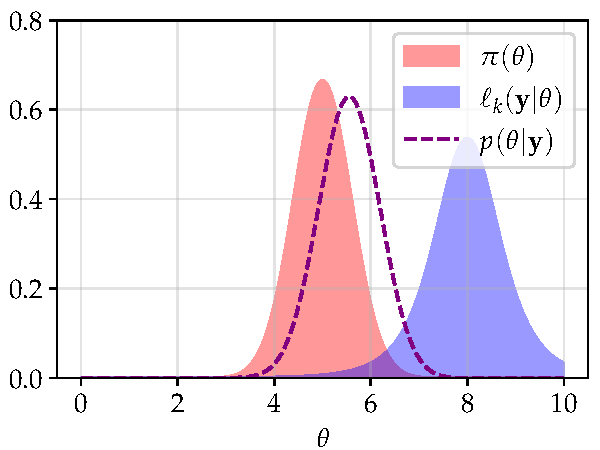
\includegraphics[width=5cm]{figures/intro/posterior1.pdf}
    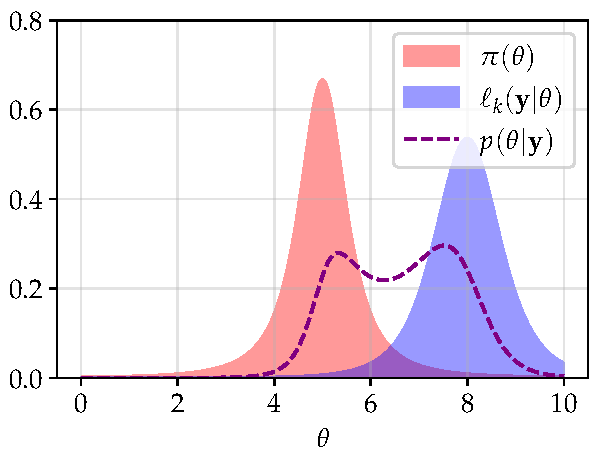
\includegraphics[width=5cm]{figures/intro/posterior2.pdf}
    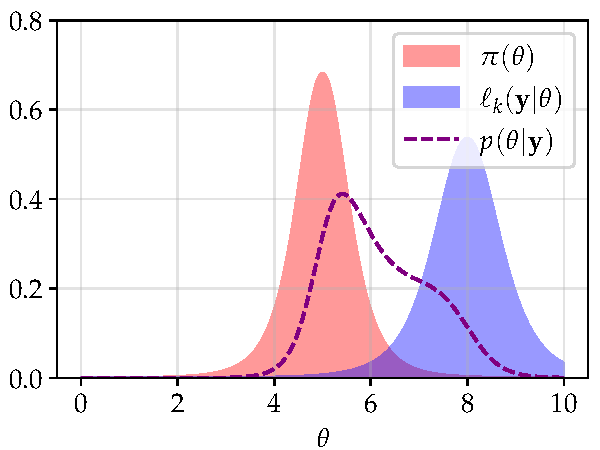
\includegraphics[width=5cm]{figures/intro/posterior3.pdf}   
    \caption{Différents calculs de posteriors (en pointillé) à partir d'une même vraisemblance (bleu) mais de différents priors (rouge).%De gauche à droite le prior est : une gaussienne $\cN(5,)}
    }
    \label{fig:intro-differentsposteriors}
\end{figure}


%On peut déduire d'un tel exemple que les queue de distribution repésente une information décisive au sein d'un prior. Cela illustre 

La question de la construction du prior reste une question ouverte dans la littérature. %tout le worflow bayésien \citep{gelman_bayesian_2020}, elle oppose souvent deux répons%es possibles
%Elle oppose souvent deux axes de refléxions : la définiton de p
Pour certains, elle est l'opportunité d'ajouter de l'information provenant d'une source extérieure, il peut s'agir d'un jugement d'expert, de données historiques, ou de connaissances sur certaines propriétés attendues du résultat. Leurs priors sont plutôt qualifiés d'informatifs.
Pour d'autres, elle est au contraire le moyen d'introduire une incertitude dans le modèle, l'\emph{a priori} est alors dans un tel cas une absence de connaissance, qui vient laisser l'information provenir essentiellement des données. Ces derniers ont confiance en la modélisation de la vraisemblance, et leur prior sera qualifié de non-informatif.


On comprend au travers de ces paragraphes introductifs que cette question est insoluble : il ne peut pas exister de méthode unanime de sélection de prior. Elle illustre même l'un des ``trous'' du workflow bayésien selon \citet{gelman_holes_2020} : les priors trop informés ne permettent pas d'avoir confiance en le moindre résultat tandis que les priors trop peu informés %n'exerguent que trop peu d'estimation crédible.
donnent lieu a des zones de crédibilité parfois trop larges et inutilisables.
%Il ne s'agit pas de décrédibiliser le bayésien 
Ce n'est pas pour autant que l'approche bayésienne perd son intérêt et cette section n'est pas vouée à discréditer la démarche, la suite du manuscrit le prouvera. %Comme toute méthode elle doit être construite 
Mais elle doit laisser celui ou celle qui l'emploie conscient ou consciente des impacts et des limites de ses choix. Le choix d'un prior est aussi critique que le choix du modèle lui-même.








%Lorsque l'on observe plusieurs réalisations de $Y$ sont observées : $(Y_1,\dots,Y_k)$






\subsection{Ce qui motive la recherche sur l'élicitation de priors pour les études sismiques probabilistes de sûreté}

L'analyse bayésienne a gagné en popularité dans de nombreux domaines, y compris dans des études de fiabilité ou de sûreté. 
En effet, elle est plébiscitée pour sa capacité (i) à introduire et propager une incertitude dans un problème d'inférence, et (ii) à être plus régulière que beaucoup de méthodes fréquentistes, en particulier lorsque le nombre de données observées est limité.

Le cadre de l'inférence bayésienne s'introduit en effet bien dans la démarche de quantification d'incertitudes. 
L'identification des incertitudes sur l'entrée $\mbf X$ ou sur le modèle même $\cM$ (ou bien s'il y a lieu le méta-modèle) peut se faire au travers d'une paramétrisation de celles-ci, en donnant lieu à une distribution paramétrique de $Y$ : $\PP_{Y|\mbf X,\theta}$.
La variable $\theta$, aléatoire sous le paradigme bayésien, peut alors représenter diverses sources d'incertitudes, de différentes natures selon les cas \citep{bousquet_contributions_2024}. Cette approche a été employée à pléthore dans divers types de modèles, on peut citer par exemple le cas de processus gaussiens (par ex. \cite{gu_parallel_2016}) ou des réseaux de neurones \citep{arbel_bayes_2023}. 



Parfois, certaines études adoptent la démarche pour la possibilité qu'elle offre d'introduire un jugement  ou une connaissance \emph{a priori}.
C'est pourtant ce même point qui fait aussi débat puisqu'il est la potentielle source d'une subjectivité difficile à justifier.
Dans le cadre des études sismiques probabilistes de sûreté en industrie nucléaire, la démonstration de robustesse est centrale. Les cas d'études y étant souvent très complexes, on trouvera alors parfois autant de priors qu'il y a d'experts en suivant cette démarche.
De tels cas caricaturaux mettent en péril l'auditabilité de la moindre région de crédibilité \emph{a posteriori}.

%De fait, il est essentiel de se chercher à se prévaloir 
%De telles études, compatibles et 
%nécessite l'apport d'un cadre méthodique et rigoureux de 

On comprend en fait que dans une étude de sûreté qui se veut auditable, une ``bonne'' région de crédibilité sur un paramètre estimé n'est pas une région nécessairement étroite, même si elle suggère que la sûreté est satisfaite. A l'inverse, une région trop large n'est pas pour autant ``bonne'' car elle ne permet pas de démontrer la robustesse attendue de l'équipement. L'équilibre est complexe, et le ``bon'' prior est celui qui, bien que démontrant au mieux la capacité ou l'incapacité de l'équipement à résister à l'aléa, produit un résultat inspirant confiance. %Il doit être assuré qu'il est affranchi de l'introduction d

Toutes ces réflexions mettent en lumières l'intérêt d'une construction méthodique du prior dans le cadre des études sismiques probabilistes de sûreté, au travers d'un cadre rigoureux qui évite l'introduction de la moindre subjectivité dans la démarche.










\section{Esquisse du manuscrit et contributions}

\subsection{Problématiques et plan}

% \subsubsection{Problématiques}


Plusieurs questions principales se détachent de cette introduction et de ces premières réflexions. Elles sont listées ci-dessous, et décrivent les problématiques majeures qui se sont manifestées au cours de cette thèse et auxquelles les travaux présentés dans ce manuscrit cherchent à répondre.


\ques{i}{Comment peut-on définir et appuyer l'objectivité d'un prior ?\\ }

\ques{ii}{Quelles sont les limites de l'emploi d'un tel prior, peu informatif par essence, et comment concilier son usage avec les besoins pratiques ?}

\ques{iii}{Comment construire et implémenter de tels priors dans un cas pratique ?\\ }

\ques{iv}{Dans le contexte des études sismiques probabilistes de sûreté, comment s'implémentent ces priors objectifs dans un modèle concret d'estimation de fiabilité sismique ?}

\ques{v}{Quelles conséquences peuvent avoir le manque d'information \emph{a priori} ou provenant des données dans ce modèle et comment les solutionner ?}

\ques{vi}{Comment peut-on finalement bénéficier au mieux des différentes sources d'information dans le workflow bayésien du modèle étudié dans son ensemble ?}\\


Dans cette thèse, nous tentons de répondre à ces six problématiques au travers d'une étude selon deux axes. Le premier axe a une dimension qualifiée de théorique, en adressant les problématiques liées à la construction de prior dits ``objectifs'' dans son ensemble. Il se concentre sur le développement d'une théorie appelée la théorie des priors de référence. Le second axe est alors plutôt qualifié de pratique, en étudiant la mise en œuvre des développements théoriques sur des cas d'études réels, en se concentrant sur l'estimation de courbes de fragilité sismiques, qui représentent un outil important du cadre des études sismiques probabilistes de sûreté.
Il reste important de rappeler que, bien qu'indépendants, les deux grands axes de travail sus-mentionnés s'alimentent l'un l'autre. Ce sont autant les problématiques pratiques qui ont motivé les recherches théoriques, que les découvertes pratiques qui ont permis les études pratiques.\\


%l'un étant plutôt théorique et adresse les questions de construction, de définiton, et d'objectivité des priors ; l'autre étant plut
% Ainsi, la premère partie de ce manuscrit est 




La \textbf{\cref{part:ref-theory}} de ce manuscrit est alors dévouée au développement de la théorie des priors de référence.

\noindent
Dans le \cref{chap:intro-ref}, on introduit la théorie et on développe son état-de-l'art. Il permet d'introduire la notion de prior de référence telle qu'elle est communément définie dans la littérature, et leur place parmi les priors objectifs. Ce chapitre permet aussi de formaliser le cadre mathématique de travail pour la suite de la partie.

\noindent
Dans le \cref{chap:ref-generalized}, on observe que la définition des priors de référence s'appuie sur une mesure de dissimilarité. On cherche alors dans ce chapitre à généraliser la définition de cette dernière afin d'appuyer le caractère objectif des priors de référence. Ce chapitre apporte une réponse à la \textbf{question i}.

\noindent
Dans le \cref{chap:constrained-prior}, on cherche une ouverture au cadre des priors de référence, lorsqu'il donne lieu à des priors difficilement utilisables en pratique. On propose alors une définition de ce qu'on appelle priors de référence contraints. Les solutions de cette définition apportent une réponse à la \textbf{question ii}.

\noindent
Dans le \cref{chap:varp}, on développe une méthode numérique d'approximation des priors de référence. Cette méthode s'appuie sur l'inférence variationnelle en définissant le prior comme la sortie d'un réseau de neurones, afin d'éviter un calcul explicite de celui-ci. Ce chapitre apporte une réponse à la \textbf{question iii}. \\


La \textbf{\cref{part:spra}} de ce manuscrit aborde le sujet de l'estimation bayésienne dite objective des courbes de fragilité sismiques.

\noindent
Dans le \cref{chap:frags-intro}, on introduit les courbes de fragilité sismiques, leur définition, leur historique et leur intégration dans le cadre des études sismiques probabilistes de sûreté. Un état-de-l'art des méthodes d'estimation de ces courbes suivant les différents types de données à disposition y est proposé.

\noindent
Dans le \cref{chap:prem}, on propose un calcul et une étude en profondeur du prior de référence pour un modèle classique employé pour l'estimation de ces courbes de fragilité. L'inférence bayésienne via l'emploi de ce prior y est comparé à d'autres méthodes. Ce chapitre apporte une réponse à la \textbf{question iv}.

\noindent
Dans le \cref{chap:constrained-frags}, on s'intéresse en profondeur aux limites du modèle considéré pour l'estimation des courbes de fragilité. On propose une solution qui est appuyée par les développements théoriques de la première partie. Ce chapitre apporte une réponse à la \textbf{question v}.

\noindent
Dans le \cref{chap:doe}, on termine notre étude en proposant une méthode qui vient appuyer l'estimation bayésienne en optimisant l'information issue des données non plus seulement  lors du choix du prior mais également lors de la sélection de celles-ci, au travers d'une méthode de planification d'expériences. Ce chapitre apporte une réponse à la \textbf{question vi}.\\


Une conclusion générale viendra clore le manuscrit dans une \textbf{\cref{part:conclusion}} finale.


\subsection{Liste des contributions}

La recherche conduite au cours de cette thèse a donné lieu à plusieurs contributions dans la littérature scientifique. Ci après sont listés les travaux publiés pendant celle-ci.

\nocite{van_biesbroeck_design_2024,van_biesbroeck_generalized_2024,van_biesbroeck_influence_2023,van_biesbroeck_properly_2024,van_biesbroeck_reference_2024,baillie_variational_2025}

\begin{itemize}
    \item \textbf{A. Van Biesbroeck}, C. Feau \& J. Garnier (2025). ``Design of experiments for efficient and conform Bayesian learning of seismic fragility curves''. \emph{Proceedings of the 28th conference on Structural Mechanics in Reactor Techology (SMiRT).}
    \item N. Baillie, \textbf{A. Van Biesbroeck}, C. Feau \& C. Gauchy (2025). ``Bayesian estimation of seismic fragility curves based on variational reference priors using neural networks''. \emph{Proceedings of the 6th Thematic Conference on Uncertainty Quantification in Computational Sciences and Engineering (UNCECOMP)}.
    \item \textbf{A. Van Biesbroeck}, C. Gauchy, C. Feau \& J. Garnier (2025). ``Robust a posteriori estimation of probit-lognormal seismic fragility curves via sequential design of experiments and constrained reference prior''. \emph{arXiv} 2503.07343. \textsc{doi:} \href{https://dx.doi.org/10.48550/arXiv.2503.07343}{10.48550/arXiv.2503.07343}.
    \item N. Baillie, \textbf{A. Van Biesbroeck} \& C. Gauchy (2025). ``Variational inference for approximate reference priors using neural networks''. \emph{arXiv} 2502.02364. \textsc{doi:} \href{https://dx.doi.org/10.48550/arXiv.2502.02364}{10.48550/arXiv.2502.02364}
    \item \textbf{A. Van Biesbroeck} (2024). ``Properly constrained reference priors decay rates for efficient and robust posterior inference'', \emph{arXiv} 2409.13041. \textsc{doi:} \href{https://dx.doi.org/10.48550/arXiv.2409.13041}{10.48550/arXiv.2409.13041}
    \item \textbf{A. Van Biesbroeck}, C. Gauchy, C. Feau \& J. Garnier (2025). ``Design of experiments based on a low fidelity model for seismic fragility curves estimation''. \emph{ESAIM: ProcS} (to appear). \textsc{hal:} \href{https://hal.science/hal-04719458v1}{hal-04719458v1}
    \item \textbf{A. Van Biesbroeck} (2023). ``Generalized mutual information and their reference priors under Csizar f-divergence''. \emph{arXiv} 2310.10530. \textsc{doi:} \href{https://dx.doi.org/10.48550/arXiv.2310.10530}{10.48550/arXiv.2310.10530}
    % \item C. Gauchy, \textbf{A. Van Biesbroeck}, C. Feau \& J. Garnier (2023). ``Inférence variationelle de lois a priori de référence''. \emph{Proceedings des 54èmes Journées de Statistiques (JdS)}. \textsc{url}
    \item \textbf{A. Van Biesbroeck}, C. Gauchy, J. Garnier \& C. Feau (2023). ``Connections between reference prior theory and global sensitivity analysis, an illustration with f-divergences''. \emph{Proceedings des 54èmes Journées de Statistiques (JdS)}. \textsc{hal:} \href{https://hal.science/hal-04171446}{hal-04171446}
    \item \textbf{A. Van Biesbroeck}, C. Gauchy, C. Feau \& J. Garnier (2023). ``Influence of the choice of the seismic intensity measure on fragility curves estimation in a Bayesian framework based on reference prior''. \emph{Proceedings of the 5th Thematic Conference on Uncertainty Quantification in Computational Sciences and Engineering (UNCECOMP)}, pp. 94-111. \textsc{doi:} \href{https://dx.doi.org/10.7712/120223.10327.19899}{10.7712/120223.10327.19899}
    \item \textbf{A. Van Biesbroeck}, C. Gauchy, C. Feau \& J. Garnier (2024). ``Reference prior for Bayesian estimation of seismic fragility curves''. \emph{Probabilistic Engineering Mechanics}, 76, pp 103622. \textsc{doi:} \href{https://dx.doi.org/10.1016/j.probengmech.2024.103622}{10.1016/j.probengmech.2024.103622}
\end{itemize}





















%Pour répondre à ces problématiques, 



  % What are the ways to define objectively a prior? Are they totally objective? Are the objective priors the most intersting priors to consider, or should we discriminate judiciously some class of priors? How to compute and implement the objective priors? 
    % What does they look like in the context of SPRA? How to use them in that context and what are the obstacles of the Bayesian approach in the context? 










\newpage
\renewcommand{\chaptername}{Chapter}
\renewcommand{\partname}{Part}



\part{Contribution to the reference prior theory}\label{part:ref-theory}
% \renewcommand{\chaptername}{Chapter}
% \renewcommand{\partname}{Part}

\chapter{Review of the reference prior theory}\label{chap:intro-ref}





\section{Introduction}

\section{The standard Bayesian framework}

\section{Prior elicitation: an open literature}

\subsection{Examples, methods, motivations}

\subsection{Informative or non-informative priors? Objective priors and mutual information}


\subsection{Limitations of the State-of-the-art}

\section{A framework for Bayesian inference with improper priors}

\subsection{Definitions and concepts}


\subsection{The reference prior theory in the appropriate framework, review of the definitions and the properties of the reference priors}



%\section{The concept of objective priors and the role of mutual information}

%\section{Reference prior definition and properties}


\section{Open paths and conclusion}


This section should conclude the state-of-the-art and delimit the limitations of the current theory on different aspects. 














\chapter{Generalized mutual information and their reference priors}\label{chap:ref-generalized}


\section{Introduction and motivations}


\section{Generalized mutual information}

\subsection{Definitions and developments}

\subsection{Motivating $f$-divergences}


\section{Generalized reference priors}

\subsection{Definitions}

\subsection{Results when $\delta<0$}

\subsection{Results when $\delta>0$}


\section{Discussions}

    \subsection{About the assumptions and their limitations}


    \subsection{About the robustness of Jeffreys prior with different divergences}


        \subsubsection{When $\delta=0$}

        \subsubsection{A heuristic for other $f$-divergences}

        \subsubsection{A simple development with a Maximum Mean Discrepancy divergence}

\section{Conclusion and prospects}
















\chapter{Properly constrained generalized reference~priors}\label{chap:constrained-prior}



\begin{abstract}[\hspace*{-10pt}]
    This chapter draws mainly on the submitted work: \fullcite{van_biesbroeck_properly_2024}  % Ce chapitre reprend principalement les travaux publiés dans: 
\end{abstract}

\begin{abstract}
    Reference priors are widely recognized for their objective nature. Yet, they often lead to intractable and improper priors, which complicates their application.
Besides, informed prior elicitation methods are penalized by the subjectivity of the choices they require. %to be made.
In this chapter, we aim at proposing a reconciliation of the aforementioned aspects. Leveraging the objective aspect of reference prior theory, we introduce two strategies of constraint incorporation to build tractable reference priors.
One provides a simple and easy-to-compute solution when the improper aspect is not questioned, and the other introduces constraints to ensure the reference prior is proper, or it provides proper posterior.
Our methodology emphasizes the central role of Jeffreys prior decay rates in this process, and the practical applicability of our results is demonstrated using an example taken from the literature.
\end{abstract}

\minitoc



\section{Introduction}\label{sec:BA:intro}


The reference prior theory represents a widely elected theory for constructing priors that are qualified as ``objective''.
The theory has been thoroughly introduced in the \cref{chap:intro-ref}. %It defines priors that maximize the impact of the observed data over themselves in the posterior definition.
The theory provides a formal mechanism to incorporate prior information in a way that maximizes the information gained from the data within the issued \emph{a posteriori} quantities.
In opposition with a plethora of existing  methods for building a prior (see e.g. \cite{mikkola_prior_2023}), 
this process is tuned to prevent the incorporation of subjective beliefs in the workflow.


However, despite their  objective nature,  their implementation is often cumbersome and not always recommended in high dimensions \citep{berger_overall_2015}. %Moreover, 
Moreover, the low-informative nature of these priors is associated with their common improper aspect, necessitating careful handling to ensure valid statistical inference.
Thus, the construction of priors is expected to strike a balance between several criteria. While many works restrict their sets of priors to ones that are tractable, proper, or suitable for high dimensions, others seek to minimize any source of subjectivity.

This chapter aims to reconcile all these criteria to improve the prior elicitation.
Our contribution takes the form of an enrichment of the reference prior theory to leverage the objective aspect that it provides to reference priors. Building on the developments presented in \cref{chap:ref-generalized},
we restrict priors to the ones that belong to  well-chosen ---and not too restrictive--- sets, and we introduce two strategies to define  convenient reference priors.
% First 
Our first strategy provides a simple,  tractable solution for constraining reference priors when the improper aspect is not questioned. The second, by contrast, introduces constraints that lead to  reference priors that are proper, or lead to proper posteriors. 
% 
For both strategies, we try to define the potential loss of objectivity induced by the constraints and we discuss their limits.
Our results emphasize the central role of Jeffreys prior decay rates when they are improper.
Additionally, we draw attention to the fact that our methodology opens a way to define various reference priors on the basis of constraints that could result from any other motivation.



This chapter is organized as follows.
In \cref{sec:BA:defsnotsmots}, after reviewing briefly the notations for the generalized reference priors framework, we develop our motivation and the objective of this work. This section is also the occasion to introduce a novel definition that is useful for the rest of the study: the quasi $D$-reference priors.
Our main results on constrained reference priors are presented in \cref{sec:BA:ress}, and discussed in \cref{sec:BA:discu}.
Then, the  practical aspect of our work is studied by the application of our method to an example taken from  the literature in \cref{sec:BA:exa}. Detailed mathematical proofs are compiled in \cref{sec:BA:proofs}. \Cref{sec:BA:conclusion} terminates the chapter with a conclusion.


\section{Definitions, notations and motivation}\label{sec:BA:defsnotsmots}

\subsection{Notations}\label{sec:BA:nots}

% \subsection{}

% notations IM, results of preceeding chapters, quasi-reference priors

%motivations %maybe its whole section

    %\subsection{The limitations of Jeffreys prior}

    %\subsection{}

In this work we consider a statistic model characterized by a collection of probability distributions $(\PP_{Y|\theta})_{\theta\in\Theta}$ on  a measurable set $(\cY,\sY)$. 
We consider the same construction of the Bayesian framework as in the \cref{chap:intro-ref} (\cref{sec:intro-refs:limits}): considering any prior $\varPi$ (that is a $\sigma$-finite measure on $\Theta$) we denote $\mbf Y_k$ a random vector of $k$ observations whose distribution conditionally to $T=\theta$ is $\PP_{\mbf Y^k|\theta}=\PP_{Y|\theta}^{\otimes k}$, where $T$ is an r.v. whose distribution is the prior $\varPi$.

The modeling is supposed to be regular: we assume $\Theta\subset\RR^d$ with $\nu$ being the Lebesgue measure on $\RR^d$ and every prior $\varPi$ is supposed to admit a density $\pi$ w.r.t. $\nu$ (i.e. $\varPi\in\sM^\nu$).
We also assume that the model admits a likelihood, denoted by $\ell$ with for any $\theta\in\Theta$ and $\mbf y\in\cY^k$, $\ell_k(\mbf y|\theta):= \prod_{i=1}^k\ell(\mbf y|\theta)$. We suppose that it verifies \cref{assu:intro-ref:jeffreysexist} in \cref{chap:intro-ref}, making the Fisher information matrix (denoted $\cI$) and the Jeffreys prior (whose density is denoted $J$) being well-defined.
The marginal distribution (resp. density)  is denoted by $\PP_{\mbf Y_k}$ (resp. $p_{\mbf Y_k}$) and the posterior distribution (resp. density) given the observations $\mbf y\in\cY^k$ is denoted by $\PP_{T|\mbf y}$ (resp. $p(\cdot|\mbf y)$).



Given these notations, we recall the expression of the generalized mutual information, defined in the \cref{chap:ref-generalized}:
\begin{equation}
    \sI_D^k(\varPi) := \EE_{T\sim\varPi}[D(\PP_{\mbf Y_k}||\PP_{\mbf Y_k|T} )],
\end{equation}
with $D$ being a dissimilarity measure.
In this chapter, we mostly focus on such generalized mutual information when $D$ is a $\delta$ divergence with $\delta\in(0,1)$. For some $\delta\in(0,1)$, the notation $D_\delta$ will refer to the $\delta$-divergence whose expression is reminded below:
    \begin{equation}
        D_\delta(P||Q) = \int_\cX f_\delta\left( \frac{p(x)}{q(x)}  \right) q(x) d\omega(x)\quad \text{with}\quad f_\delta(x) = \frac{x^\delta-\delta x-(1-\delta)}{\delta(1-\delta)},
    \end{equation}
where $p,q$ respectively are densities pf $P$ and $Q$ w.r.t. a common measure $\omega$ on $\cX$.
When evoking reference priors in a general way, we will refer to generalized reference priors, as proposed in the \cref{chap:ref-generalized}.
We remind below their definition:
\begin{defi}[Generalized reference prior]\label{def:BA:genref}
    Let $D$ be a dissimilarity measure and $\cP$ a set of priors on $\Theta$. A prior $\varPi\in\cP$ is called a $D$-reference prior over $\cP$ with rate $\varphi(k)$ if there exists an openly increasing  sequence of compact subsets $(\Theta_i)_{i\in\NN}$
    such that $\bigcup_{i\in\NN}\Theta_i=\Theta$ and for any $i$: $0<\varPi(\Theta_i)<\infty $ and
    % with $\pi^\ast(\Theta_i)>0$, $\Theta_i\subset\Theta$, $\bigcup_{i\in I}\Theta_i=\Theta$ such that
        \begin{equation} %\label{eq:defrefpriorsi}
            \lim_{k\rightarrow\infty}\varphi(k)[\sI^k_D(\varPi(\cdot|\Theta_i))-\sI^k_D(P(\cdot|\Theta_i))] \geq0 \text{\ for all\ } P\in\cP\text{\ verifying\ }0<P(\Theta_i)<\infty;
        \end{equation}
    where  $\varphi(k)$ is a {positive and}  monotonous function of $k$. It is said to be unique if for any other $D$-refernce prior $\varPi'$, $\varPi\simeq\varPi'$.
\end{defi}

We also remind the following result on the $D_\delta$-mutual information and their reference priors (see \cref{chap:ref-generalized}).
%  that are defined considering a generalized ,
\begin{thm}\label{thm:BA:l(pi)}
    Suppose $\Theta$ to be compact and $\varPi\in\sM^\nu_\cC$ be a prior with $\varPi(\Theta)=1$. the $D_\delta$-mutual information admits a limit:
        \begin{equation}
            \lim_{k\rightarrow\infty} k^{d\delta/2} \sI_{D_\delta}(\varPi) = l(\pi) - (\delta(1-\delta))^{-1}, \quad l(\pi) = C_\delta \int_{\Theta}\pi(\theta)^{1+\delta} |\cI(\theta)|^{-\delta/2}  d\theta ,
        \end{equation}
        where $\pi$ is the density of $\varPi$, and with $C_\delta= (2\pi)^{d\delta/2} (1-\delta)^{-d/2}/(\delta(\delta-1))$.\\
    Call $\cR\subset\sR_{\cC^b}$ a set of densities such that $M(\cR)=\cP$, with $M$ mapping a density to its associated prior. Then
        $\varPi$ is a $D_\delta$-reference prior over $\cP$ iff $\pi$ maximizes $l$ over $\cR$. 
\end{thm}




\subsection{Objective and motivation}\label{sec:BA:mots}



We already know that the definition of the reference prior and the $D_\delta$-reference prior is satisfied by the Jeffreys prior over the large set of priors $\sM^\nu_\cC$ in most cases (see \cref{chap:intro-ref,chap:ref-generalized}).
% in most case (see \cref{chap:intro-ref} for ). 

%the large set of priors admitting locally bounded and a.e. continuous densities w.r.t. the Lebesgue measure \citep{VanBiesbroeckBA2023}. 

This result is, however, limiting and disappointing in some cases. The reasons are the following ones: (i) the Jeffreys prior is not recommended in high-dimensional problems as it is known to be ``either too diffuse or too concentrated'' \citep{berger_overall_2015}; moreover (ii) when the expression of the likelihood is itself complex, the computation of the Jeffreys prior can become  intractable; %which is why (iii) in practice a restriction to the set of priors to ones which are easier to compute is often favored; 
also (iii) the Jeffreys prior is known to often lead to an improper prior, which does not necessarily issue a proper posterior distribution, essential for practical \emph{a posteriori} inference and sampling.

To tackle these limitations, we propose in this work to restrict the set of priors over which we derive the reference priors.
Indeed, the reference prior definition is usually considered with very large sets of priors, which are constrained only by some regularity assumptions imposed to the priors (such as continuity, positivity). These regularity assumptions do not generally discriminate the Jeffreys prior from the studied set of priors.
In this chapter, different restricted sets of priors will be suggested, they are sets that are though 
to counter the limitations (ii) and (iii) aforementioned. In most cases, they will not include the Jeffreys prior.
%to not include the Jeffreys prior when 



The tackling of limitation (i) mentioned above is not a purpose of this work. We recall that it is actually frequently tackled a sequential construction of the reference prior as %presented in \cref{chap:intro-ref} (\cref{sec:intro-ref:refpriors}).
suggested by \citet{bernardo_reference_1979}.
On the condition that an ordering of the parameters is set:
 \begin{equation}
     \theta = (\theta_1,\dots,\theta_r) \in \Theta=\Theta_1\times\dots\times\Theta_r,
 \end{equation}
this construction considers a hierarchical construction of the reference prior.
It is already described in \cref{chap:intro-ref} (\cref{sec:intro-ref:refpriors}). We remind below the steps of the sequential construction:
%
%Typically, it is recommended to assume $\Theta_j\subset\RR^{d_j}$ with small dimensions $d_j$ (e.g., lower or equal than $2$) for any $j\in\{1,\dots,r\}$, and to sequentially build a reference prior on the $\Theta_j$,  $j\in\{1,\dots,r\}$:
 \begin{enumerate}
     \item initially fix $\ell_k^1=\ell_k$;
     \item for any values of $\theta_{j+1},\dots,\theta_r\in\Theta_{j+1}\times\dots\times\Theta_r$, compute a reference prior (in the sense of \cref{def:intro-ref:ref-priors})  under the model with likelihood $\theta_j\mapsto\ell_k^j(\mbf y|\theta_j,\dots,\theta_r)$, denote $\pi_j(\cdot|\theta_{j+1},\dots,\theta_r)$ its normalized density;
     \item derive $\ell_k^{j+1}$ such as 
         \begin{equation} %\label{eq:hier:condlikeint}
            \ell_k^{j+1}(\mbf y|\theta_{j+1},\dots,\theta_r) =  \int_{\Theta_j}\ell_k^j(\mbf y|\theta_j,\dots,\theta_r)d\pi_j(\theta_j|\theta_{j+1},\dots,\theta_r).
         \end{equation}
 \end{enumerate}

In this work, the reference priors will be derived only given their formal definition (\cref{def:BA:genref}). Yet, our results can be incorporated in this sequential construction. Indeed,
step 2 of the method depicted above consists of the derivation of a reference prior w.r.t. the variable $\theta_j$.
%in the sense of 
% Thus, our reference priors over constrained setes of priors can be  plainly incorporated into this method.
Additionally, we invite to note that this construction does not solve the limitations (ii) and (iii) previously evoked. Actually, it makes them essential. Indeed, step 2 requires, firstly, a derivation of a reference prior, so that it would lead to a low-dimensional Jeffreys prior if the set of priors is not constrained. Also step 3 necessitates, secondly, that the latter leads to a proper posterior so that the integral involved does not diverge.

We note that this last issue is taken into account by \citet{berger_development_1992} with the suggestion of such construction on an increasing sequence of compact subsets of $\Theta$: $\bigcup_{i\in\NN}\Theta_i=\Theta$. The hierarchical reference prior can then be chosen as a limit of the ones obtained under $\Theta_i$ when $i\to\infty$. However, this limit can be cumbersome to derive in practice. Another solution suggested by \citet{mure_objective_2018} is to restrict the $\sigma$-algebra $\sY$ until the reference prior derived in step 2 leads to a proper posterior. It is still imperfect, as there is no guarantee that such a restricted $\sigma$-algebra exists outside the trivial one.


%In the following subsections, we propose a range of solutions to some of the issues aforementioned, based on the derivation of reference priors over constrained setes of priors. In  Section  {sec:constrainedasympt}, we derive a quasi $D_\delta$-reference prior over setes of priors that are easy to compute, in order to tackle the limitations (ii) and (iii) previously evoked. Then, Section  {sec:constrainedproper} explores another kind of constrained setes of priors, which leads to $D_\delta$-reference priors that can solve the item (iv).












\subsection{A useful definition: quasi-reference priors}\label{sec:BA:defsquas}

%As explained in the introduction, the objective of this work is to study reference priors over restricted sets of priors. Indeed, the reference prior definition is usually considered with very large sets of priors, which are constrained only by some regularity assumptions imposed to the priors (such as continuity, positivity). %This regularity does not generally discriminate the Jeffreys prior
%Actually, 
%The choice of the set of priors $\cP$ in \cref{def:BA:genref} remains open and can be restrained from the large one of priors in $\cM^\varrho_\cC/\!\simeq$. %admitting continuous densities w.r.t. the Lebesgue measure.

While we aim at restricting the set of priors $\cP$ in \cref{def:BA:genref}, we must notice
that such a restriction leaves really unsure the existence of a reference prior. 
Indeed, the definition is itself restrictive, as to admit a reference prior, the set $\cP$ must contain a prior whose restrictions are optimal on any compact subsets of $\Theta$.
In this section, we suggest an extension of the definition of reference priors in the case where in the set $\cP$, the optimal priors on compact subsets of $\Theta$ are not renormalization of each other, but converge to a  prior in $\cP$. 
Such convergence is considered in the sense of the Q-vague convergence \citep{bioche_approximation_2016} on $\sM^\nu_\cC$. % on $\cM^\nu\cC/\!\simeq$. This convergence defines a topology 
The Q-vague convergence of a sequence $(\varPi_n)_n$ to a limit $\varPi$ is equivalent to the convergence of $([\varPi_n])_n$ to $[\varPi]$ in $\sM^\nu_\cC/\!\simeq$ for the quotient topology of the vague convergence on $\sM^\nu_\cC$.




\begin{defi}[Quasi reference prior]\label{defi:quasiRefprior}
    Let $\cP$ be a set of priors. We call $\varPi\in\cP$ a quasi $D$-reference prior if it exists an openly increasing sequence $(\Theta_i)_{i\in \NN}$  of compact sets with $\bigcup_{i\in\NN}\Theta_i=\Theta$ such that
    \begin{itemize}
        \item[(i)] for any $i\in \NN$, there exists a $D$-reference prior $\varPi_i$ over $\cP_i=\{P(\cdot|\Theta_i),\, P\in\cP,\,P(\Theta_i)\in(0,\infty) \}$, %, the set of renormalized restrictions to $\Theta_i$ of priors in $\cP$,
        \item[(ii)] $\varPi$ is the Q-vague limit of the sequence $(\varPi_i)_{i\in \NN}$.
    \end{itemize}
    It is said to be unique  if for any other quasi $D$-reference prior $\varPi'$, $\varPi\simeq\varPi'$.
\end{defi}

Proposition below ensures that this definition properly extends \cref{def:BA:genref} in the case of $\delta$-divergences.
\begin{prop}\label{prop:quasi}
     \begin{itemize}
        \item If $\varPi$ is a $D_\delta$-reference prior over a set $\cP$, then it is a quasi $D_\delta$-reference prior.
        \item If $\cP$ is a set of priors convex and stable by multiplication by indicator functions over measurable sets, then the quasi $D_\delta$-reference prior over $\cP$ is the unique $D_\delta$-reference prior over $\cP$.
        \item If $\cP$ is a convex set of priors and if the sequence of subsets $(\Theta_i)_i$ in \cref{def:BA:genref} is fixed, then the quasi-reference prior over $\cP$ is unique.
    \end{itemize}
\end{prop}


\begin{proof}
    The first statement of the proposition is clear given the definition of a $D_\delta$-reference prior.\\
    For the second, let us adopt the notations of \cref{thm:BA:l(pi)} and  notice that if $\Theta$ is compact and if $\pi^\ast$ is the maximal argument of $l$ over $\cR$, then its renormalized restriction $\pi_1^\ast$ on a compact subset $U$ maximizes $l$ over the set of all renormalized densities $\cR_U$.
    Indeed, if we suppose that $\pi_1\in\cR_U$ maximizes $l$ then, denoting $\pi_0^\ast$ the renormalized restriction of $\pi^\ast$ to $\Theta\setminus U$, $t=\int_U\pi^\ast$, and $\pi = t\pi_1+(1-t)\pi_0^\ast$, $\pi\in\cR$ and
        \begin{equation}
            l(\pi) = t^{\delta+1}l(\pi_1) + (1-t)^{\delta+1}l(\pi_0^\ast) > t^{\delta+1}l(\pi_1^\ast) + (1-t)^{\delta+1}l(\pi_0^\ast) = l(\pi^\ast).
        \end{equation}
    Hence $\pi^\ast$ does not maximize $l$ over $\cR$, which is absurd.\\
    Therefore, in our problem, considering two sequences $(\pi^{(1)}_i)_i$ and $(\pi_i^{(2)})_i$ respectively defined on $(\Theta_i^{(1)})_i$ and $(\Theta^{(2)}_i)_i$, we will get that for any $i$, $\pi^{(1)}_i(\theta)=\pi_i^{(2)}(\theta)$ for all $\theta\in\Theta_i^{(1)}\cap\Theta_i^{(2)}$. Eventually, they are identical on every compact subsets of $\Theta$, and equal to their Q-vague limits which are the same.\\
    Finally, the third statement of the proposition results from the strict concavity of $l$. Indeed, for any $i$, the set $\cR_i$ of renormalized restricted densities on $\Theta_i$ is convex so that the maximal argument of $l$ over $\cR_i$ is unique. Hence the uniqueness of the quasi-reference prior over $\cP$.
\end{proof}
    



\section{Constrained $D_\delta$-reference priors}\label{sec:BA:ress}





\subsection{Constrained $D_\delta$-reference priors based on Jeffreys' asymptotic decay rates}\label{sec:BA:res1}



    % \subsection{Results}

    


    In this section, we tackle the computational cost of the reference prior. As mentioned in \cref{sec:BA:mots}, the Jeffreys prior expression is often complex to derive even in low dimensional models. This is even more a problem in practical studies where the prior must be evaluated a numerous number of times, when it resorts to MCMC simulations to provide posterior samples of $\theta$ for instance.

    In some works of the literature, the Jeffreys prior is replaced by its decay rates at the boundary of the domain. For instance, the reference prior for Gaussian processes suggested by \citet{gu_jointly_2019} is built on the basis of the decay rates of a Jeffreys prior sequentially computed on the different variables that compose $\theta$ (following the construction presented in \cref{sec:BA:mots}).
    Their idea is that, in particular when it is improper, the prior provides the most information from its asymptotic rates, and variations of them are noticed to have a strong influence on the posterior distribution.
    The result that follows provides a formalization of this intuition, focusing on the case where the Jeffreys prior asymptotically behaves like exponentiation of coordinates of $\theta$.
    
    
    
    
    
    \begin{thm}\label{thm:Jthetaa}
        Suppose $\Theta\subset\RR$ is an interval of the form $[c,b)$ (or $(b,c]$). Call $M:\pi\in\sR_{\cC^b}\mapsto(B\mapsto\int_B \pi d\nu)\in\sM^\nu_\cC$. %, with $J$ integrable and non-null in the neighborhood of $c$.
        \begin{itemize}
            \item If $b\in\RR$ and $J(\theta)\equi{\theta\rightarrow b}C|\theta-b|^a$ for constants $C\in\RR$ and $a\leq-1$, then $M(\pi^\ast)$ where $\pi^\ast(\theta)\propto|\theta-b|^a$ is the unique quasi $D_\delta$-reference prior over $M(\hat\cR)$ where $\hat\cR = \{\pi(\theta)\propto|\theta-b|^u,\,u\in\RR\}$.
            \item If $|b|=\infty$ and $J(\theta)\equi{\theta\rightarrow b}C\theta^a$ for constants $C\in\RR$ and $a\geq-1$, then $M(\pi^\ast)$ where $\pi^\ast(\theta)\propto\theta^a$ is the unique quasi $D_\delta$-reference prior over $M(\hat\cR)$ where $\hat\cR = \{\pi(\theta)\propto\theta^u,\,u\in\RR\}$.
        \end{itemize}
    \end{thm}
    
    \begin{proof}
        The proof is technical and detailed in \cref{sec:BA:proofs}.
        The idea is that $l(\pi)$ can be seen as a negative divergence between $\pi$ and $J$. However, when $J$ is improper at the boundary of the domain, the maximization of $l(\pi)$ gets closer to the minimization of a divergence between $\pi$ and the improper decay rate of $J$.
    \end{proof}
    
    
    \begin{rem}
        \Cref{thm:Jthetaa} still stands when $\Theta=(b,c)$ (or $(c,b)$) if $c\ne\infty$ and if $J(\theta)$ admits a non-null and finite limit when $\theta\to b$.
    \end{rem}
    
    
    
    
    This theorem serves the statement of two conclusions: (i) it emphasizes that when Jeffreys prior is improper, its improper decay rates contain the most relevant information, and (ii) it proposes to choose this asymptotic expansion of Jeffreys as a quasi $D_\delta$-reference prior when we look for an easy prior to compute.
    
    
    






\subsection{Properly constrained $D_\delta$-reference priors}\label{sec:BA:res2}



In \cref{sec:BA:res1}, we have provided some elements to construct a tractable reference prior on the coordinates over which Jeffreys prior is improper.
The reference prior that our theorem proposes keeps the improper characteristic of Jeffreys prior on the same coordinates.
This improper aspect can, however, remain an issue in some cases, especially when the resulting posterior is improper as well.

For this reason, it might happen that some asymptotic rates in some directions still have to be tackled. The work in this section is concluded by results that allow defining a $D_\delta$-reference prior (or quasi $D_\delta$-reference prior), which benefits from adjusted decay rates from Jeffreys prior. 
The proposition below constitutes a preliminary result that gives the form of a $D_\delta$-reference prior over a set of priors with linear constraints.

\begin{assu}\label{assu:glibre}
    A family of functions from $\Theta$ to $\RR$ $(g_j)_{j=1}^p$ is said to satisfy \cref{assu:glibre} if $g_0,\dots,g_p$ are linearly independent in the space of a.e. continuous functions from $\Theta$ to $\RR$, where $g_0:=\theta\mapsto 1$.
\end{assu}

\begin{prop}\label{prop:constraints}
    Suppose $\Theta$ to be a compact subset of $\RR^d$. Let $g_1,\dots,g_p$ be %a.e. continuous 
    functions in $\sR_{\cC^b}$ %from $\Theta$ to $\RR$ 
    that satisfy \cref{assu:glibre}. Define $\tilde\cP$ the set of priors $\varPi$ on $\Theta$ such that $\forall 1,\dots,p$, $\int_\Theta g_jd\varPi=c_j$, for some $c_j\in\RR$.
    If %$\tilde\cP$ is not empty, then 
    there exists a $D_\delta$-reference prior over $\tilde\cP$, it is unique. If it is positive, its density $\pi$ verifies
    \begin{equation}
        \pi(\theta) = J(\theta)\left(\lambda_0+\sum_{j=1}^p\lambda_jg_j(\theta) \right)^{1/\delta},
    \end{equation}
    for some $\lambda_j\in\RR$. Reciprocally, if there exists a prior %$\pi^\ast\in\tilde\cP$ 
    whose density verifies the above equation for some $\lambda_j\in\RR$, it is the $D_\delta$-reference prior over $\tilde\cP$.
\end{prop}

\begin{proof}
    This proposition results from a Lagrange multipliers theorem. A detailed proof is proposed in \cref{sec:BA:proofs}.
\end{proof}



\begin{rem}
    While it is not the subject of this work, we let the reader notice that this proposition opens the way to the introduction of constraints based on expert judgments in prior elicitation. They can take the form of moment constraints or predictive constraints. %\citep{bousquet_contributions_2024}.    
\end{rem}

\begin{rem}\label{rem:klconst}
    The expression of the reference prior given by \cref{prop:constraints} depends on the chosen $\delta$-divergence.
    While this work considers only the framework of reference priors under $\delta$-divergences as a dissimilarity measure, a version of this theorem could be written in the original framework of the reference prior theory that uses the Kullback-Leibler divergence. The expression of the resulting reference prior would be impacted. 
    In the appendix we prove that the expression using the Kullback-Leibler divergence would take the form:
    %In \cite{bernardo_bayesian_1994}, the authors suggest that the expression should take the form of
        \begin{equation}
            \pi^\ast\propto J\cdot\exp\left(\sum_{j=1}^p\lambda_j g_j\right),
        \end{equation}
        for some $\lambda_j$ that remain to be determined.
    This expression was already intuited by \citet{bernardo_bayesian_1994}.
        %Their suggestion is supported by the derivations made in \cite[\S C.3, Theorem 2]{GauchyPhD}.
\end{rem}
 



Below, given a function $g$ that is selected to adjust the asymptotics of Jeffreys prior, is stated the expression of a proper $D_\delta$-reference prior.

\begin{thm}\label{thm:lintoproper}
    Let $g:\Theta\to(0,\infty)$ be a function in $\sR_{\cC^b}$ such that
        \begin{equation}\label{eq:intgalphafinite}
            \int_\Theta J(\theta)g^{1/\delta}(\theta)d\theta<\infty \quad\text{and}
            \quad\int_\Theta J(\theta)g^{1/\delta+1}(\theta)d\theta<\infty,
        \end{equation}
    and suppose that $g$ is bounded in the neighborhood of $b$ for an element $b\in\partial\Theta$. %such that $J$ is improper in the neighborhood of $b$.
    We denote by $\overline\cP$ the set of positive priors $\varPi$ on $\Theta$ such that $\int_\Theta gd\varPi<\infty$, and we define 
    $\varPi\in\overline\cP$ as the prior whose density $\pi$ verifies % follows 
        \begin{equation}
            \pi(\theta)\propto J(\theta)g(\theta)^{1/\delta}.
        \end{equation}
    If $Jg$ is non-integrable in the neighborhood of $b$, then $\varPi$ is a $D_\delta$-reference prior over $\overline\cP$. Otherwise, and if $J$ is improper in the neighborhood of $b$, $\varPi$ is a $D_\delta$-reference prior over the set of proper priors in $\overline\cP$.
\end{thm}

\begin{proof}
    The statement of this theorem results from the sequential use of \cref{prop:constraints} on an increasing sequence of compact subsets of $\Theta$. A detailed proof is written in \cref{sec:BA:proofs}.     
\end{proof}


%\begin{rem}
   To improve the above theorem, one would like 
     to relax the first assumption in \cref{eq:intgalphafinite}, i.e., to let $\int_\Theta J g^{1/\delta}$  be infinite. Indeed, in this way, the result would provide a reference prior $\varPi$ ---non-necessarily proper--- but such that $\pi g\in L^1$, where $\pi$ is a density of $\varPi$. With a good choice of $g$, $\pi^\ast$ could be built as a prior that provides a proper posterior. It is the purpose of the next theorem. 
    The cost of this relaxation is the provision of a quasi-reference prior instead of a reference prior.
    %However, our proof needs this assumption, but one can feel that such (quasi)-reference prior is not far to exist as expressed in the proposition  below.
%\end{rem}

\begin{thm}\label{thm:quasipostpropre}
    Let $g:\Theta\to(0,\infty)$ be in $\sR_{\cC^b}$ such that
    \begin{equation}
        \int_\Theta J(\theta)g(\theta)d\theta=\infty\quad\text{and}\quad \int_\Theta J(\theta)g^{1/\delta+1}(\theta)d\theta<\infty,
    \end{equation}
and suppose that $g(\theta)\conv{\theta\rightarrow b}0$ for an element $b\in\partial\Theta$ such that $J$ is non-integrable in the neighborhood of $b$.\\
Let $(\Theta_i)_{i\in\NN}$ be an openly increasing sequence of compact sets that covers $\Theta$ and $(c_i)_i$ be a bounded sequence in $(0,\infty)$. Define the set of priors  $\overline\cP'=\{\varPi,\,\forall i,\,\int_{\Theta_i} gd\varPi=c_i\int_{\Theta_i}d\varPi\}$.\\ %, where $(c_i)_i$ is a bounded sequence in $(0,\infty)$.\\
Denote for any $i$ $\overline{\cP}'_i$ the set of renormalized restrictions to $\Theta_i$ of priors in $\overline{\cP}'$. If for any $i$ there exists a  positive maximum of $l$ over $\overline\cP'_i$, then  $\varPi$ whose density is denoted $\pi$ is a quasi $D_\delta$-reference prior over $\overline\cP'$ with
    \begin{equation}
        \pi(\theta)\propto J(\theta)g(\theta)^{1/\delta}.
    \end{equation}
    This prior is such that $\int_\Theta\pi gd\nu<\infty$.
\end{thm}




\section{Discussion}\label{sec:BA:discu}

The knowledge of Jeffreys prior's decay rates is central in the results presented in this work. These results indicate that in common scenarios where Jeffreys prior is improper, these rates must be explicitly considered in order to construct a reference prior. 

We let the reader note that \cref{thm:lintoproper,thm:quasipostpropre} introduce results that also depend on the chosen dissimilarity measure. Therefore, a balance must be found between the subjective influence of the constraint and the quest for an informed prior to facilitate possible sampling from the posterior. This is illustrated in the example we address in the following section.
However, it is important to observe that using the KL-divergence instead of a $\delta$-divergence %considered in our work 
would result in a stronger influence of the constraint on the final prior. As noted in \cref{rem:klconst}, the exponentialization of the function $g$ could lead to a prior with distribution tails that are significantly negligible beyond those of Jeffreys, thereby jeopardizing its objective nature.

Generally, the results we propose in \cref{sec:BA:res1,sec:BA:res2} address different problems and are thus  fundamentally different in nature. In one case, the improper aspect of Jeffreys prior is not necessarily challenged, and an efficient construction of the latter is proposed. In the other case, the goal is to significantly attenuate its improper aspect while maintaining as much objectivity as possible. In this latter case, however, the expressions of the proposed  reference priors still depend on the expression of Jeffreys prior. Nevertheless, when Jeffreys prior is proper, there is no guarantee that a straightforward construction inspired by its convergence rates at the domain boundaries will be relevant. %ensure its reference nature in a simple and interpretable way. 
Indeed, although improper tails concentrate an infinite mass that constitutes all the information at the boundaries, when they are proper, the information of interest may need to be sought elsewhere. In this case, a calculation or approximation of the `proper' Jeffreys prior remains to be considered.

Finally, regarding \cref{thm:Jthetaa}, although the result is limited to parameter power distribution tails, it is observed that, in practice, these include a wide range of improper Jeffreys priors.
For example, this includes Jeffreys priors derived from various Gaussian models, such as those introduced by \citet{neyman_consistent_1948}; Jeffreys priors related to specific parameters within Gaussian process models \citep{gu_parallel_2016}; and those arising in more specialized contexts, like the one %
that we develop in the \cref{part:spra} of this manuscript.
%in \cite{VanBiesbroeck2023}.
%
%
%are concerned the Jeffreys prior in the normal 
%\textcolor{red}{Il faudrait en lister plusieurs.}
Moreover, the invariance of Jeffreys priors under re-parameterization can sometimes allow us to return to this case. Specifically, if $J$ can be asymptotically written as a power of a function $f$, where $f$ is differentiable, monotone and with bounded derivative (from above and from below), then the re-parameterization $\vartheta=f(\theta)$ %with a well  
should allow us to recover the reference prior among those expressible as powers of $f$.

In the following section, we illustrate an application of our work with an example taken from the literature.


\section{An example}\label{sec:BA:exa}


In their work, \citet{rubio_inference_2014} prove that the two piece location-scale model they proposed has an improper Jeffreys prior, which issues an improper posterior.
The model is parameterized by $\theta=(\mu,\sigma_1,\sigma_2)\in\RR\times(0,\infty)^2$, inferred over observations in $\cY=\RR$. It has the following likelihood:
    \begin{equation}\label{eq:examplelikilihood}
        \ell(y|\theta) =  \frac{2}{\sigma_1+\sigma_2}\left[f\left(\frac{y-\mu}{\sigma_1}\right)\indic_{(-\infty,\mu)}(y) + f\left(\frac{y-\mu}{\sigma_2}\right)\indic_{(\mu,\infty)}(y)  \right],
    \end{equation}
where $f$ is a density function with support on $\RR$, assumed to be symmetric with a single mode at zero, and with a few integrability assumptions that are detailed in \cite{rubio_inference_2014}.
    The choice of $f$ is open and we can take, % let the assumptions of Theorem  {thm:l(pi)} to be verified.
    %\textcolor{red}{
    %We may take, 
    for instance, the standard Gaussian density function.
    Under this construction, the Fisher information matrix of this model takes the form:
    \begin{equation}\label{eq:fishermatrix}
        \cI(\theta) = \left(\begin{array}{ccc}
             \frac{\alpha_1}{\sigma_1\sigma_2}& -\frac{2\alpha_3}{\sigma_1(\sigma_1+\sigma_2)} & \frac{2\alpha_3}{\sigma_2(\sigma_1+\sigma_2)}  \\
             \ast &\frac{\alpha_2}{\sigma_1(\sigma_1+\sigma_2)} + \frac{\sigma_2}{\sigma_1(\sigma_1+\sigma_2)^2} & - \frac{1}{(\sigma_1+\sigma_2)^2}  \\
             \ast&\ast& \frac{\alpha_2}{\sigma_2(\sigma_1+\sigma_2)} + \frac{\sigma_1}{\sigma_2(\sigma_1+\sigma_2)^2}
        \end{array}\right)
    \end{equation}
    for some positive constants $\alpha_1$, $\alpha_2$ and $\alpha_3$.

    The full Jeffreys prior can be computed as 
    \begin{equation}
        J(\theta) \propto \frac{1}{\sigma_1\sigma_2(\sigma_1+\sigma_2)},
    \end{equation}
    it is improper and leads to an improper posterior. In the following, we construct different priors based on the suggestions developed in this chapter. %a method which, on the basis of our suggestions developed in what precedes, to construct a more suitable prior.

    \paragraph{Proper priors based on a moment constraint}
    Considering results in \cref{sec:BA:res2} and the decay rates of the Jeffreys prior above, a simple correction can be done to issue a proper reference prior w.r.t. $\sigma_1,\sigma_2$, which results in a proper posterior.
    We consider $\delta\in(0,1)$; given $\eps\in(0,\frac{1}{1+1/\delta})$ we have 
        \begin{equation}
            %\int J(\theta)(\sigma_1\sigma_2)^{\eps/\delta} d\sigma_1d\sigma_2<\infty\quad\text{and}\quad 
            \int J(\theta)(\sigma_1\sigma_2)^{\eps/\delta+1} d\sigma_1d\sigma_2<\infty,
        \end{equation}
    so that the associate proper $D_\delta$-reference prior density $\pi$, which is such that $\pi(\mu,\sigma_1,\sigma_2)\sigma_1^\eps\sigma_2^\eps$ is integrable w.r.t. $\sigma_1,\sigma_2$, is
        \begin{equation}
            \pi(\mu,\sigma_1,\sigma_2) \propto \frac{(\sigma_1\sigma_2)^{\eps/\delta -1}}{\sigma_1+\sigma_2}.        
        \end{equation}


\paragraph{Overview and sensibility on the parameters}
Our prior densities are compared with the Jeffreys prior one on \cref{fig:priorpost}.(a), w.r.t. the parameter $\sigma_2$ the others being fixed to $1$. For this comparison, a multiplicative constant had to be chosen on $J$, we have chosen the one such that $J(1,1,1)=2$.
Our priors differ as a function of $\gamma=\eps/\delta\in(0,\frac{1}{1+\delta})\subset(0,1)$. On the one hand, when $\gamma$ becomes close to $0$, the prior ---which we denote by $\pi_\gamma$ from now on--- becomes close to the Jeffreys prior, i.e., the most objective prior w.r.t. the mutual information criterion. However, in this case, $\pi_\gamma$ becomes close to an improper prior, and its posterior becomes close to an improper posterior. On the other hand, setting $\gamma$ away from $0$ 
rearranges the quantity of information in the prior. Its referential nature decreases in favor of an increase in its entropy.
%make the prior more informative, and probably more subjective. 
Therefore, a trade-off has to be made between suitability for inference and objectivity.
Finally, note that in \cref{fig:priorpost}.(a) is also drawn the \emph{independent Jeffreys prior} proposed by the authors in \cite{rubio_inference_2014} for this model as an alternative to Jeffreys. Its decay rates are actually the same as the ones of $\pi_\gamma$ when $\gamma=1/2$, and the two priors are hard to distinguish. Note that this latter prior $\pi_{1/2}$ equals the hierarchical reference prior (as described in  \cref{sec:BA:mots}) constructed from the ordering $\pi(\theta)=\pi_1(\sigma_1,\sigma_2|\mu)\pi_2(\mu)$.




To evaluate a bit further our method, we propose a visualization of the posterior sensitivity to the priors, i.e., to $\gamma$. 
Such influence quantification constitutes a critical step of the \emph{Bayesian workflow}, as expressed by   \citet{gelman_bayesian_2020}. Several methods exist  in the literature for this purpose (e.g., \cite{berger_robust_1990,nott_checking_2020}). 
An approach is to compare the variations of an \emph{a posteriori} quantity as a function of the parameter \citep{kallioinen_detecting_2023}. In this example, this methodology is yet limited by the improper aspect of Jeffreys posterior. It cannot be considered for any comparison.
In \cref{fig:priorpost}.(b), (c) and (d) are plotted, for numerous $\gamma$ and several data set sizes $k$, the posterior densities that result from a sample of data and from the prior densities $\pi_\gamma$.
%The influence of the priors can be recognized, especially for tiny values of $k$. 
As expected, the influence of the prior appears for small values of $k$.
Indeed, we can notice that for higher values of $\gamma$, the posterior is slightly more shifted to the right and seems to be a little flatter. 
It is remarkable that this observation becomes limited when $k$ increases. When $k=50$, the difference between the posterior densities 
is hard to distinguish. %limited and it is 
%The remarkable result is that all the posterior median densities are very close in this example. 
This indicates that the little losses of objectivity should induce small variations in the resulting inference in this example.

For practical details, the chosen $f$ is the standard Gaussian density, and the different data sets have been generated according to the likelihood in \cref{eq:examplelikilihood} conditionally to $\theta^\ast=(2,2,2)$. %They were of size $k=50$, and a number $N=1000$ of them have been generated for the computation of the median densities.



%%However, they are difficult to implement in this example as 
%An approach is to compare the posterior-prior divergences \citep{Nott2020}. %If evaluated and averaged for different data-set, this method amount to compare mutual information evaluations. We propose it in Figure  to illustrate the loss of `objectivity' as a function of $\gamma$.


% In Figure  another approach is considered: we plot the divergences of posteriors issued by $\pi^\ast_\gamma$ to the improper posterior issued by Jeffreys \citep{Kallioinen2023}. Those divergences are computed using $\delta$-divergence, and considering the improper density $p^J(\dot|\mbf y)$ issued by Jeffreys:
%     \begin{equation}
%         p^J(\theta|\mbf y)=J(\theta)\prod_{i=1}^k\ell(y_i|\theta),
%     \end{equation}
% with $J(\theta)$ being such that $J(1,1,1)=1$.



    
    
% \paragraph{Hierachical prior}

%    In accordance with the criticize of \citet{Berger2009} about the derivation of the Jeffreys prior on the full parameter space aforementioned in Sectio
%        \begin{equation}
%            J(\sigma_1,\sigma_2|\mu) \propto \frac{1}{\sqrt{\sigma_1\sigma_2}(\sigma_1+\sigma_2)}
%        \end{equation}
%    which is also improper as
%        \begin{equation}
%            \int_0^\infty\int_0^\infty\frac{1}{\sqrt{\sigma_1\sigma_2}(\sigma_1+\sigma_2)}d\sigma_1d\sigma_2 = \int_0^\infty \frac{2}{\sigma_2}\int_0^\infty \frac{1}{1+\gamma^2}d\gamma d\sigma_2 = +\infty
%        \end{equation}
%     (using the substitution $\gamma=\sqrt{\sigma_1/\sigma_2}$). 
    %More over, this prior also leads to an improper posterior given that
%        \begin{align}
%            \int_0^\infty\frac{2}{\sqrt{\sigma_1\sigma_2}(\sigma_1+\sigma_2)^2}f\left(\frac{y-\mu}{\sigma_2}\right)d\sigma_1 &= \int_0^\infty\frac{4}{\sigma_2^2(\gamma^2+1)^2} f\left(\frac{y-\mu}{\sigma_2}\right) d\gamma \\
%            &= \frac{\pi}{\sigma_2^2}f\left(\frac{y-\mu}{\sigma_2}\right)
%        \end{align}
%    with the quantity above being non-integrable w.r.t. $\sigma_2$ in the neighborhood of $0$.

%    Therefore, the process of the derivation of a hierarchical reference prior cannot be pursued at this point.


% $f(\sigma_1,\sigma_2)=(\gamma,\eta)=(\sigma_1/\sigma_2,\sigma_1+\sigma_2)$, $f^{-1}(\gamma,\eta)=(\gamma\eta)$, $\mathrm{Jac}\,f(\sigma_1,\sigma_2) = 1/\sigma_2,-\sigma_1/\sigma_2^2,1,1$, $\det=\frac{\sigma_1+\sigma_2}{\sigma_2^2}$

% $\int\int \frac{\sigma_1+\sigma_2}{\sigma_2^2(\sigma_1/\sigma_2)^{1/2}(\sigma_1+\sigma_2)^2\sigma_2^{-1}}=\int\int\frac{(\eta/\gamma-1)^{1/2}}{\gamma^{1/2}\eta^2}$


    


\begin{figure}[h]%
    \centering%
    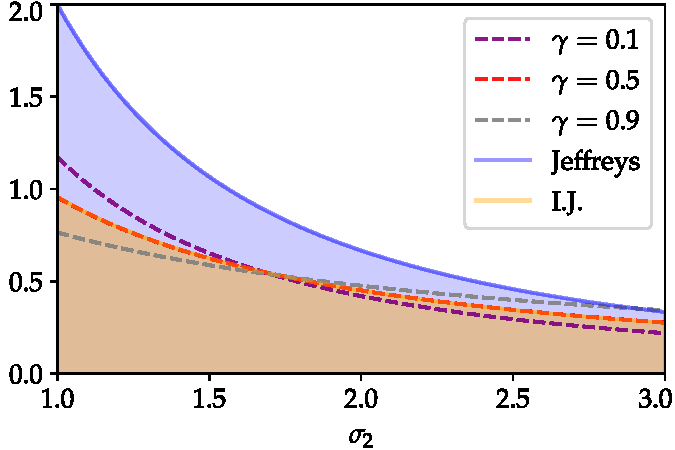
\includegraphics[width=6cm]{figures/constrained-priors/priors_.pdf}\hspace*{1cm}%
    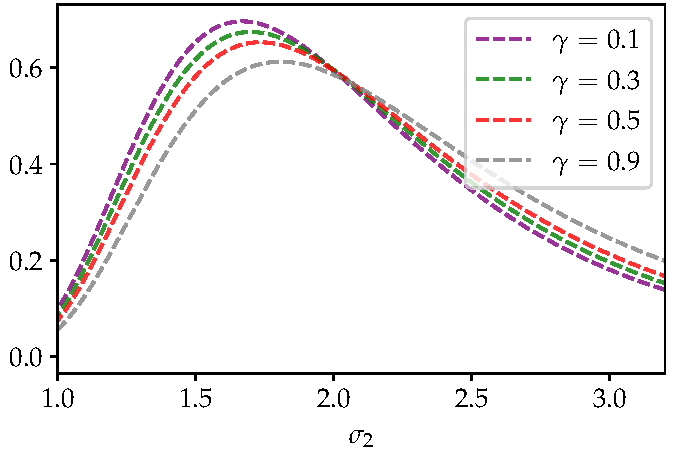
\includegraphics[width=6cm]{figures/constrained-priors/post5.pdf}\\
    \makebox[13cm][c]{%
    {~\hspace{\stretch{1}}(a)\hspace{\stretch{2}}(b)\hspace{\stretch{1}}~}}\\[5pt]
    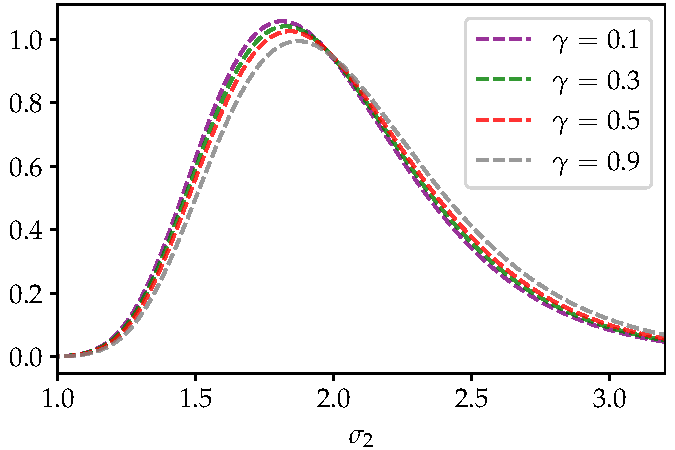
\includegraphics[width=6cm]{figures/constrained-priors/post15.pdf}\hspace*{1cm}%
    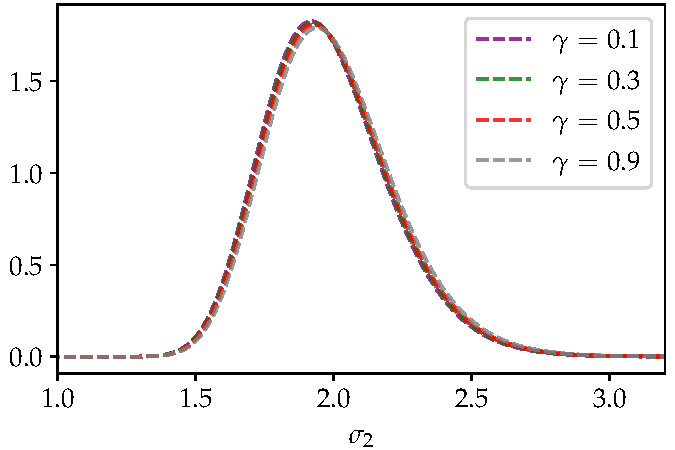
\includegraphics[width=6cm]{figures/constrained-priors/post50.pdf}\\
    \makebox[13cm][c]{%
    {~\hspace{\stretch{1}}(c)\hspace{\stretch{2}}(d)\hspace{\stretch{1}}~}}%
    \caption{On (a), different prior densities $\pi_\gamma$ (in dashed line) w.r.t. $\sigma_2$ along with a Jeffreys prior density (that delimits the blue area) and the \emph{Independent Jeffreys} of \cite{rubio_inference_2014} (that delimits the orange area). On each of (b), (c) and (d), posterior densities for different values of $\gamma$ are plotted. %One observed sample served the calculation of all the posteriors on one figure. 
    One observed sample was used to calculate all the posteriors in a figure.
    The observed sample has a size of $k=5$ in (b), $k=15$ in (c), and $k=50$ in (d).\label{fig:priorpost}}
\end{figure}








\section{Detailed proofs}\label{sec:BA:proofs}


\subsection{Proof of \cref{thm:Jthetaa}}

To prove this theorem, we consider to simplify the derivations that $b=0$ with $\Theta=(0,1]$. We will show later how to extend the result to the other cases. As the Jeffreys prior can be defined up to a positive multiplicative constant with no incidence on the definition of a $D_\delta$-reference prior, 
we will simplify its decay rate assuming $J(\theta)\equi{\theta\rightarrow 0}\theta^a$.

Let us define the increasing sequence of compact subsets $\Theta$: $\Theta_i=[\theta_i,1]$, $i\geq0$, with $\theta_i\conv{i\rightarrow\infty}0$. We denote by $\psi_i$ and $\tilde\psi_i$ the functions defined as follow:
    \begin{equation}
        \psi_i(u) = -\frac{\int_{\Theta_i}J(\theta)^{-\delta}\theta^{u(1+\delta)}d\theta }{\left(\int_{\Theta_i}\theta^ud\theta \right)^{1+\delta}},\qquad \tilde\psi_i(u) = -\frac{\int_{\Theta_i}\theta^{-a\delta }\theta^{u(1+\delta)}d\theta }{\left(\int_{\Theta_i}\theta^ud\theta \right)^{1+\delta}}.
    \end{equation}
The quantity $\psi_i(u)$ corresponds ---up to a positive constant--- to the parametrization w.r.t. $u\in\RR$ of $l(\pi_i)$; where $\pi(\theta)\propto\theta^u$, $\pi_i$ is re-normalized restriction of $\pi$ to $\Theta_i$  and where $l$ is the function defined in \cref{thm:BA:l(pi)} that we seek to maximize.
Therefore, if we call $u_i\in\argmax_{u\in\RR}\psi_i(u)$ for any $i$, and if the associated sequence of priors $(M(\pi_i))_i$ converge Q-vaguely to a prior $\varPi^\ast$ over $\Theta$, that would prove that $\varPi^\ast$ is a quasi $D_\delta$-reference prior.

\paragraph{The case $\mathbf{a<-1}$}
    Firstly, we assume that $a<-1$. Denote $U=(-\infty, u_m:=\frac{\delta a-1}{1+\delta})$, we want to derive an asymptotic equivalent when $i\to\infty$ of $\psi_i(u)$, uniformly w.r.t. $u\in U$.
    More precisely, we are about to show that for any $\eps>0$ there exists a $i_1$ such that for any $u\in U$ and $i>i_i$, $|\psi_i(u)-\tilde\psi_i(u)|<\eps|\tilde\psi_i(u)|$. %\theta_i^{-\delta(a+1)}$.
    

    Let $\eps>0$, using that $J(\theta)^{-\delta}\equi{\theta\rightarrow0}\theta^{-\delta a}$, there exists $i_0$ such that for any $\theta<\theta_{i_0}$, $|J(\theta)^{-\delta}-\theta^{-\delta a}|<\eps\theta^{-\delta a}$. %for a $\tilde\eps$ that we determine later.
    Now, we consider an $i_1$ such that: % for any $u\in U$:
        \begin{equation}
            \frac{\int_{\Theta_{i_0}}J(\theta)^{-\delta}d\theta }{\int_{\theta_{i_1}/\theta_{i_0}}^1J(\theta_{i_0}\theta)^{-\delta}\theta^{u_m(1+\delta)} d\theta}<\theta_{i_0}\eps/2\quad \text{and}\quad
            \frac{\int_{\Theta_{i_0}}\theta^{-\delta a}d\theta }{\int_{\theta_{i_1}/\theta_{i_0}}^1(\theta_{i_0}\theta)^{-\delta a}\theta^{u_m(1+\delta)} d\theta}<\theta_{i_0}\eps/2.
        %
            % \frac{\int_{\Theta_{i_0}} J(\theta)^{-\delta}\theta^{u(1+\delta)}  d\theta}{\int_{\Theta_{i_1}\setminus\Theta_{i_0} } J(\theta)^{-\delta }\theta^{u(1+\delta)}d\theta }
            % = 
            % \frac{\theta_{i_0}^{-1}\int_{\theta_{i_0}}^1 J(\theta)^{-\delta}(\frac{\theta}{\theta_{i_0}})^{u(1+\delta)}  d\theta}{\int_{\theta_{i_1}/\theta_{i_0}}^1 J(\theta_{i_0}\tilde\theta)^{-\delta }\tilde\theta^{u(1+\delta)} d\tilde\theta }
            % %
            % < \frac{\theta_{i_0}^{-1}\int_{\Theta_{i_0} }J(\theta)^{-\delta} d\theta}{\int_{\theta_{i_1}/\theta_{i_0} }^1 J(\theta_{i_0}\theta)^{-\delta }\theta^{u^m(1+\delta)}d\theta}
        \end{equation}
    Thus, for any $i>i_1$  and any $u\in U$:
        \begin{equation}
            \frac{\int_{\Theta_{i_0}} J(\theta)^{-\delta}\theta^{u(1+\delta)}  d\theta}{\int_{\Theta_{i}\setminus\Theta_{i_0} } J(\theta)^{-\delta }\theta^{u(1+\delta)}d\theta }
            = 
            \frac{\theta_{i_0}^{-1}\int_{\theta_{i_0}}^1 J(\theta)^{-\delta}(\frac{\theta}{\theta_{i_0}})^{u(1+\delta)}  d\theta}{\int_{\theta_{i}/\theta_{i_0}}^1 J(\theta_{i_0}\theta)^{-\delta }\theta^{u(1+\delta)} d\theta } %\\
            %
            < \frac{\theta_{i_0}^{-1}\int_{\Theta_{i_0} }J(\theta)^{-\delta} d\theta}{\int_{\theta_{i_1}/\theta_{i_0} }^1 J(\theta_{i_0}\theta)^{-\delta }\theta^{u_m(1+\delta)}d\theta} < \eps/2
        \end{equation}
    and
        \begin{equation}
            \frac{\int_{\Theta_{i_0}} \theta^{-\delta}\theta^{u(1+\delta)}  d\theta}{\int_{\Theta_{i}\setminus\Theta_{i_0} } \theta^{-\delta }\theta^{u(1+\delta)}d\theta }
            = 
            \frac{\theta_{i_0}^{-1}\int_{\theta_{i_0}}^1 \theta^{-\delta}(\frac{\theta}{\theta_{i_0}})^{u(1+\delta)}  d\theta}{\int_{\theta_{i}/\theta_{i_0}}^1 (\theta_{i_0}\theta)^{-\delta }\theta^{u(1+\delta)} d\theta } %\\
            %
            < \frac{\theta_{i_0}^{-1}\int_{\Theta_{i_0} }\theta^{-\delta} d\theta}{\int_{\theta_{i_1}/\theta_{i_0} }^1 (\theta_{i_0}\theta)^{-\delta }\theta^{u_m(1+\delta)}d\theta} < \eps/2,
        \end{equation}
    so that $|\psi_i(u)-\tilde\psi_i(u)|<\tilde\eps|\tilde\psi_i(u)|$ as expected. %Finally, deriving $\tilde\psi_i(u)$ gives
        %\begin{equation}
         %   |\psi_i(u)-\tilde\psi_i(u)|<\tilde\eps  |u+1|^\delta K\theta_i^{-\delta(a+1)}\frac{1-\theta_i^{-(\delta(u-a)+u+1)}}{(1-\theta_i^{-u-1})^{1+\delta}} <\tilde\eps |u+1|^\delta K'\theta_i^{-\delta(a+1)}
        %\end{equation}        
    %for some constants $K,\,K'>0$, using that $\theta_i^{-u-1}\leq\theta_i^{-u_m-1}<1$ and that$\theta_i^{-(\delta(u-a)+u+1)}\leq\theta_i^{-(\delta(u_m-a)+u_m+1)}\leq1$. Hence the expected result when $\tilde\eps=\eps/K$.

    Now we want to use this asymptotic equivalence to bound the difference $|a-u_i|$, where $u_i$ is defined as a maximal argument of $\psi_i$. The next step is thus to show that such $(u_i)_i$ exists.
    
    There exist $\tilde K$, $\tilde K'$ such that $\tilde K\theta^{-\delta}\leq J(\theta)^{-\delta}\leq \tilde K'\theta^{-\delta}$. 
    Let $i\geq0$, we can write
        \begin{equation}\label{eq:gendarmeJeffreys}
            \tilde K |\tilde\psi_i(u)| \leq|\psi_i(u)| \leq \tilde K'|\tilde\psi_i(u)|
        \end{equation}
    with 
        \begin{equation}
            |\tilde\psi_i(u)| = \theta_i^{-\delta(a+1)}\frac{|u+1|^{1+\delta}}{|\delta(u-a)+u+1|}\frac{1-\theta_i^{-\delta(u-a)-u-1}}{(1-\theta_i^{-u-1})^{1+\delta}}  \conv{u\rightarrow-\infty}+\infty.
        \end{equation}
    That makes $|\psi_i|$ being a coercive and continuous function on $U$, so that it admits minimal arguments in $U$. We denote by $u_i$ one of them: 
        \begin{equation}
            u_i \in \argmax_{u\in U} \psi_i(u).
        \end{equation}

    We recall that, by concavity of $x\mapsto -x^{-\delta}$, we find that $a$ is the only maximal argument of $\tilde\psi_i$ for any $i$. 
    This way, for $i>i_1$, we write
        \begin{align}
            |\tilde\psi_i(u_i)-\tilde\psi_i(a)|&\leq |\psi_i(u_i)-\tilde\psi_i(u_i)| +  |\psi_i(a)-\tilde\psi_i(a)| + |\psi_i(u_i)-\psi_i(a)| \nonumber\\
            \tilde\psi_i(a) - \tilde\psi_i(u_i) &%\leq \eps(|u_i+1|^\delta+ |a+1|^\delta) \theta_i^{-\delta (a+1)} + \psi_i(u_i)-\psi_i(a),
            \leq \eps(|\tilde\psi_i(u_i)|+|\tilde\psi_i(a)|)+ \psi_i(u_i)-\psi_i(a),
        \end{align}
    which leads to 
        \begin{align}
            2(\tilde\psi_i(a)-\tilde\psi_i(u_i)) &%\leq  \eps(|u_i+1|^\delta+ |a+1|^\delta) \theta_i^{-\delta (a+1)} + \psi_i(u_i)-\tilde\psi_i(u_i)+\tilde\psi_i(a)-\psi_i(a) \nonumber\\
            \leq \eps(|\tilde\psi_i(u_i)|+|\tilde\psi_i(a)|) +  \psi_i(u_i)-\tilde\psi_i(u_i)+\tilde\psi_i(a)-\psi_i(a) \nonumber\\
            \tilde\psi_i(a) - \tilde\psi_i(u_i) &%\leq \eps (|u_i+1|^\delta+ |a+1|^\delta) \theta_i^{-\delta (a+1)}.
            \leq \eps(|\tilde\psi_i(u_i)|+|\tilde\psi_i(a)|).
        \end{align}
    %The above work allows to conclude that
    %Within the last inequality above, 
    Consequently to the convergence of
     $(\theta_i^{\delta(a+1)}\tilde\psi_i(a))_i$ toward a positive limit when $i\to\infty$, we deduce that $\theta_i^{\delta(a+1)}(\tilde\psi_i(a)-\tilde\psi_i(u_i))/|\theta_i^{\delta(a+1)}\tilde\psi_i(u_i)|$ is asymptotically null. This prevents the sequence $(\theta_i^{\delta(a+1)}\tilde\psi_i(u_i))_i$ to admit a non finite subsequential limit, meaning it has to be bounded and to converges to the same limit as $(\theta_i^{\delta(a+1)}\tilde\psi_i(a))_i$, i.e. $-|a+1|^\delta$.

     On another hand, we notice that for any $M>0$, there exist a $M'$ such that for any $u<M'$, 
        \begin{equation}
            \frac{|u+1|^{1+\delta}}{|\delta(u-a)+u+1|}>M
        \end{equation}
     and $|\theta^{\delta(a+1)}\tilde\psi_i(u)|>M$ for any $i\geq0$. Thus, as $(\theta^{\delta(a+1)}\tilde\psi_i(u_i))_i$ has been proven to be bounded, so must be $(u_i)_i$.

     To conclude on that sequence, we denote by $\rho$ a finite subsequential limit of $(u_i)_i$, if $\rho\ne u_m$ then deriving the limit of $\theta^{\delta(a+1)}\tilde\psi_i(u_i)$ leads to 
        \begin{align}
           & -\frac{|\rho+1|^{1+\delta}}{\delta(\rho-a)+\rho+1} = |a+1|^\delta \nonumber\\
           \text{i.e.}\quad & -|\rho+1|(|\rho+1|^\delta-|a+1|^\delta) = |a+1|^\delta \delta(\rho-a);
        \end{align}
    necessarily, $\rho=a$.
    It remains to prove that $\rho=u_m$ is absurd. Indeed, in this case the integrals $\int_{\Theta_i}\theta^{-\delta a+u_i(1+\delta)}d\theta$ converge either to $0$, either to $+\infty$. Therefore, that would make $(\theta_i^{\delta(a+1)}\tilde\psi_i(u_i))_i$ converging either to $-\infty$, either to $0$, which in both case is different to $-|a+1|^\delta$.


    %Eventually, $(u_i)_i$ converges to $a$.

    Let us now work beyond the subset $U$ of $\RR$. First, if $u\in(-1,+\infty)$, the integrals that compose $\psi_i(u)$ both admit finite and positive limits when $i\to\infty$. The limit of $(|\psi_i(u)|)_i$ is moreover bounded from below as a consequence of \cref{eq:gendarmeJeffreys}:
        \begin{equation}\label{eq:minorationpsiu1infty}
            |\psi_i(u)|\geq \tilde K\frac{(u+1)^{1+\delta}}{ \delta(u-a)+u+1}\frac{1-\theta_i^{\delta(u-a)+u+1}}{(1-\theta_i^{u+1})^{1+\delta}} \geq \tilde K'|\log\theta_i|^{-1-\delta}.  %{(\mu+1)^{\delta}}. %\conv{i\rightarrow\infty}\infty
        \end{equation}
    %and the same way, $\psi_i(-1)\geq\tilde K\frac{(\log\theta_i)^{-1-\delta}}{|\delta(1+a)|}$
    Thus, there exists $i_2\geq0$ such that for any $i>i_2$ $|\psi_i(a)|<\tilde K'|\log\theta_i|^{-1-\delta}$, consequently to $\psi_i(a)\equi{i\rightarrow\infty}|a+1|^{\delta}\theta_i^{-\delta(a+1)}\aseq{i\rightarrow\infty}o(|\log\theta_i|^{-\delta-1})$.
    As a result, for any $i>i_2$:
        \begin{equation}
            \sup_{u\in(-1,+\infty)}\psi_i(u)<\psi_i(a)\leq\psi_i(u_i).
        \end{equation}
    Finally, if $u\in(u_m,-1)$, analogously than in \cref{eq:minorationpsiu1infty}, we can write
        \begin{equation}
            |\psi_i(u)|\geq\tilde K(u+1)^{1+\delta}\frac{|\log\theta_i|}{(1-\theta_i^{u+1})^{1+\delta}} \geq \tilde K''\theta_i^{-(u_m+1)(1+\delta)}|\log\theta_i|^{-\delta}.
        \end{equation}
    Once again, we have $\psi_i(a)\aseq{i\rightarrow\infty}o(\theta_i^{-(u_m+1)(1+\delta)}|\log\theta_i|^{-\delta})$ and we can consider $i_3\geq 0$ such that for any $i>i_3$:
        \begin{equation}
            \sup_{u\in(u_m,-1)}\psi_i(u)<\psi_i(a)\leq\psi_i(u_i).
        \end{equation}

    All the work that precedes proves that any sequence $(v_i)_i$ defined by $v_i\in\argmax_{\RR}\psi_i$ converges to $a$.
    

\paragraph{The case $\mathbf{a=-1}$}
In this case, we easily get that $\psi_i(a)\equi{i\rightarrow\infty}-|\log\theta_i|^{-\delta}$. 
When $u<\eta<a$, 
    \begin{equation}
        |\psi_i(u)|\geq\tilde K\frac{|u+1|^{\delta}}{\delta+1} \frac{1-\theta_i^{-(\delta+1)(u+1)}}{(1-\theta_i^{-u-1})^{1+\delta}}\geq \hat K {|\eta+1|^{\delta}}(1-\theta_i^{-(\eta-1)({1+\delta})})
    \end{equation}
and when $u>\tilde\eta>a$,
    \begin{equation}
        |\psi_i(u)|\geq\tilde K\frac{|u+1|^{\delta}}{\delta+1} \frac{1-\theta_i^{(\delta+1)(u+1)}}{(1-\theta_i^{u+1})^{1+\delta}}\geq \hat K' {|\tilde\eta+1|^{\delta}}(1-\theta_i^{(\tilde\eta-1)({1+\delta})}).
    \end{equation}


Thus, for any $\eps>0$, the equations above with $\eta=a-\eps$ and $\tilde\eta=a+\eps$ let state that there exists an $i_1\geq0$ such that for any $i>i_1$:
    \begin{equation}
        \sup_{u\in(-\infty,a-\eps)}\psi_i(u)<\psi_i(a)\quad\text{and} \quad\sup_{u\in(a+\eps,\infty)}\psi_i(u)<\psi_i(a)
    \end{equation}
so that $\argmax_{\RR}\psi_i\subset(a-\eps,a+\eps)$, which let the definition of a sequence $(u_i)_i$ of maximal arguments of $\psi_i$ which converges to $a$.


\paragraph{Q-vague convergence}
The conclusion concerning the Q-vague convergence of the $M(\pi_i^\ast)$ defined from the $u_i$ constructed in the work above: $\pi_i^\ast(\theta)\propto\theta^{u_i}$ is a direct result of \cite[Proposition 2.16]{bioche_approximation_2016}. Indeed, the convergence of sequence $(u_i)_i$ toward $a$, implies that the sequence of our priors converges Q-vaguely to $\varPi^\ast$ such that $\varPi^\ast = M(\pi^\ast)$ with $\pi^\ast(\theta)\propto{\theta^a}$.



\paragraph{Extension to other set $\Theta$}
We shall now demonstrate that the proven result extends itself to the general case: $\Theta=[c,b)$ or $(b,c]$, $b\in\RR\cup\{-\infty,\infty\}$.

We first consider $\Theta=(b,c]$ with $b\in\RR$.
We denote by $\cQ$ the set of priors densities after the substitution $\vartheta = (\theta-b)/(c-b)\in T=(0,1)$:  $\cQ=\{\tilde\pi(\vartheta) = (b-c)\pi(\vartheta (b-c)+b),\,\pi\in\hat\cR\}$.
Thus, $\cQ = \{\pi(\theta)\propto\vartheta^u,\,u\in\RR\}$.
We define the increasing sequence of compact sets $(\Theta_i)_i$ by $\Theta_i = [b+t_i,c]$ with $t_i\conv{i\rightarrow}0$. Therefore, for $\pi\in\hat\cP$, calling $\pi_i$ the renormalized restriction of $\pi$ to $\Theta_i$ gives
    \begin{equation}
        l(\pi_i) = \tilde l(\tilde\pi_i) = C_\delta\int_{T_i}\tilde\pi_i(\vartheta)^{1+\delta}\tilde J(\vartheta)^{-\delta}d\vartheta
    \end{equation}
with $T_i=[t_i,1]$, $\tilde\pi_i(\vartheta) = (b-c)\pi_i(\vartheta (b-c)+b)\in\cQ$ and $\tilde J(\vartheta) = (b-c)J(\vartheta (b-c)+b)\equi{\vartheta\rightarrow0}\vartheta^a$.
Thus, the work done above states that the family of maximal arguments $\tilde\pi_i^\ast$ of $\tilde l$ over $\cQ_i$  provides a sequence of priors $(M(\tilde\pi_i^\ast))_i$ that converges Q-vaguely toward $M(\tilde\pi^\ast)$ where $\tilde\pi^\ast(\vartheta)\propto\vartheta^a$.
Thus, the associate densities $\pi^\ast_i$ maximize $l$ over $\cP_i$ and issues a sequence of priors $(M(\pi^\ast_i))_i$ that converges Q-vaguely toward $M(\pi^\ast)$ where $\pi^\ast(\theta)\propto|\theta-b|^a$.

To treat the other cases, other substitutions with analogous work permit to conclude:
(i) the substitution $\vartheta=(b-\theta)/(b-c)$
when $\Theta=(c,b)$, $b\in\RR$; (ii) the substitution $\vartheta=1/(|\theta-c|+1)$ when 
$\Theta=[c,\infty)$ or $(-\infty,c]$.








\subsection{Proof of \cref{prop:constraints}}

Let us start by the uniqueness.
%Recall the definition of an openly increasing sequence of compact sets $(\Theta_i)_{i\in\NN}$: there exist $i_0\geq0$ and a sequence $(V_i)_{i\geq i_0}$ of open subsets of $\Theta$  such that for any $i\geq i_0$
%    \begin{equation}
%        \Theta_i\subset V_i\subset \Theta_{i+1}.
%    \end{equation}
%This way, $\bigcup_iV_i=\Theta$ and the compacity of $\Theta$ imposes it to  be a finite union, so that $\Theta_i=\Theta$ for any $i\geq i_1$ for some $i_1\geq0$.\\
%
%
%If $(\Theta_i)_{i\in \NN}$ is an increasing sequence of compact subsets that covers $\Theta$, %%%($i_1<i_2\Longrightarrow\Theta_{i_1}\subset\Theta_{i_2}$, $$), 
%it is stationary, i.e. there exist an $i_0$ such that for any $i>i_0$, $\Theta_i=\Theta$.\\ %%%finite subset $\tilde I\subset I$ such that $\bigcup_{i\in\tilde I}\Theta_i=\Theta$ (or, if $I$ is totally ordored, there exist $i_0$ such that for any $i>i_0$, $\Theta_i=\Theta$).\\
%Indeed, by contradiction assuming that for any $n$, $\bigcup_{i\leq n}\Theta_i\ne\Theta$, its complementary is non-empty and contains a non-empty closed subset $F_n\subset\left(\bigcup_{i\leq n}\Theta_i\right)^c$. Therefore, as $\Theta\subset\RR^d$ it is an Hausdorff compact set so that the two closed sets $F_n$ and $G_n=\bigcup_{i\leq n}\Theta_i$ are subsets of two disjoints open sets $U_n$ and $V_n$: $F_n\subset U_n$, $G_n\subset V_n$. This way, $\bigcup_{n\in\NN}V_n=\Theta$ and by compactness there exists $N$ such that $V_N=\Theta$ and so $F_N=\empty$ which is a contradiction.
%
%Any $D_\delta$-reference prior
A prior $\varPi^\ast\in\cP$ is a $D_\delta$-reference prior if and only if its density $\pi^\ast$ maximizes $l$ over $\cR$, where $M(\cR)=\cP$.
As the set $\cP$ is convex, $\cR$ is convex as well. Also, we notice that the function $\pi\mapsto l(\pi)$ is strictly concave, so that its maximizer is unique in the sense that two maximizer are equal $\nu$-a.e. That ensures the $D_\delta$-reference prior is unique.
%$\pi^\ast$ over a convex   such as $\tilde\cP$ must maximize $l$ as a prior on $\Theta$. The mapping $\pi\mapsto l(\pi)$ being strictly convex when $\pi$ is seen as a function in $\cR^\cC$, such maximal argument is unique.


% Regarding the expression of $\pi^\ast$,it can be seen as a direct consequence of the following lemma, which proven later on.

% \begin{lem}\label{lem:constrainstaec0}
%     Calling $U$ the set of positive and a.e. continuous function from $\Theta$ to $\RR$, and $C=\{f:\Theta\to\RR,\, \int_\Theta f=1,\,\forall j,\,\int_\Theta f_jg_j=c_j\}$, if $\pi^\ast=\argmax_{\pi\in C\cap U}l(\pi)$ exists, it verifies
%         \begin{equation}\label{eq:lemconstepiast}
%             \pi^\ast(\theta)  J(\theta)\left(\lambda_0+\sum_{j=1}^p\lambda_jg_j(\theta)\right)^{1/\delta},
%         \end{equation}
%     for some $\lambda_j\in\RR$. Reciprocally, if there exists a $\pi^\ast\in C\cap U$ that satisfies above equation for some $\lambda_j\in\RR$, then it maximizes $l$ over $C\cap U$.
% \end{lem}




% \paragraph{Proof of Lemma {lem:constrainstaec0}}
Regarding the expression of $\pi^\ast$,
let us call $E$ the space of bounded a.e. continuous functions from $\Theta$ to $\RR$ and we equip $E$ with the supremum norm over $E$: $\|f\|=\sup_\Theta|f|$. The set $\Theta$ being supposed compact, the pair $(E,\|\cdot\|)$ constitutes a Banach vector space whose restriction $U$ composed by the positive functions of $E$ is an open and convex subset.
It is possible to see $l$ as being a concave function defined on $U$.


Let us compute the differentiate of $l$ over $U$. One can write $l=\phi_2\circ\phi_1$ with
\begin{equation}
    \phi_1:\pi\in E\longmapsto \pi^{1+\delta}\in E ;\qquad \phi_2:\pi\in E\longmapsto C_\delta \int_\Theta \pi(\theta)|\cI(\theta)|^{-\delta/2}d\theta.
\end{equation}
As $\phi_2$ is a continuous linear mapping from $E$ to $\RR$, $l$ is differentiate while $\phi_1$ is, with for any $h\in E$:
    \begin{equation}
        dl(\pi) = \phi_2\circ d\phi_1(\pi).
    \end{equation}
Fix $\pi\in U$. For an $\eps>0$ there exists $\tilde\eps>0$ such that while $|x|<\|\pi\|$ and $|u|<\tilde\eps$ then $|(x+u)^{1+\delta}-x^\delta-(1+\delta)x^\delta u|<\eps|u|$. Thus for any $h\in E$ such that $\|h\|<\tilde\eps$, we have
    \begin{equation}
        \|\phi_1(\pi+h) -\phi_1(\pi)-(1+\delta)\pi^\delta h\|<\eps\|h\|.
    \end{equation}
We conclude that $\phi_1$ differentiable on $U$ with $d\phi_1(\pi)h = (1+\delta)\pi^\delta h$, for any $\pi\in U$, $h\in E$. This differentiate is additionally continuous, which makes $l$ continuously differentiable as well.

Thus, considering the additional constraint $\int_\Theta\pi(\theta)d\theta=1$, this problem can be treated applying the Lagrange multipliers theorem (see e.g. \citep{zeidler_applied_2012}) to state that there exist $\lambda_0,\dots,\lambda_p\in\RR^{p+1}$ such that
    \begin{equation}
        dl(\pi^\ast)h - \lambda\int_\Theta h(\theta)d\theta - \sum_{i=1}^p\lambda_i\int_\Theta h(\theta)g_i(\theta)d\theta = 0
    \end{equation}
for any $h\in E$. Eventually, as $dl(\pi)h=C_\delta(1+\delta)\int_\Theta\pi(\theta)^{\delta}|\cI(\theta)|^{-\delta/2}h(\theta)d\theta$, we get
    \begin{align}
        \pi^\ast(\theta) = J(\theta)\bigg(\lambda_0+\sum_{i=1}^p\lambda_ig_i(\theta)\bigg)^{1/\delta}.
    \end{align}
% with $J(\theta$

Moreover,
as $l$ is strictly concave and the constraints are linear, the second order condition for the Lagrangian states the reciprocal aspect of this result: calling $C$ the space of functions satisfying the constraints, if $\pi^\ast\in U\cap C$ satisfies the last equation above, it maximizes $l$.


%To conclude, notice that densities of non-negative priors satisfying the constraints constitute %belongs to 
%the closure of $U\cap C$, $C$ designing the set of the functions that satisfy the constraints. As $\pi^\ast$ disclosed above maximizes $l$ over $U\cap C$, with $l$ being continuous on its closure. Therefore, $\pi^\ast$ maximizes $l$ over all that latter, i.e. its associated prior is the $D_\delta$-reference prior over $\tilde\cP$.

To conclude, the elements in $\tilde\cP$ are associated to densities which belong to $E$ because $\Theta$ is compact.
They are non necessarily everywhere positive, but only supposed to be non-negative.
This set of bounded a.e. continuous and non-negative functions satisfying the constraints is actually the closure of $U\cap C$ over which $l$ is continuous.
Therefore, calling $\tilde\cP^\ast$ the set of positive priors in $\tilde\cP$, we have $\argmax_{M(\pi)\in\tilde\cP}l(\pi)=\argmax_{M(\pi)\in\tilde\cP^\ast}l(\pi)$ which is $\pi^\ast$.








\subsection{Proof of \cref{thm:lintoproper}}


Assuming that it exists, denote by $\pi^\ast$ the density of the $D_\delta$-reference prior $\varPi^\ast$ over $\overline\cP$, denote as well
    \begin{equation}
        c = \int_{\Theta}\pi^\ast(\theta)g(\theta)d\theta,\quad Z_i = \int_{\Theta_i}\pi^\ast(\theta)d\theta
    \end{equation}
for any $i\in \NN$, considering an openly increasing sequence $(\Theta_i)_{i\in\NN}$ of compact sets that cover $\Theta$ over which $1>\varPi^\ast(\Theta_i)>0$ for any $i$ such that $\Theta_i\ne\Theta$ (we show later that they exist).
In particular, $\varPi^\ast$ must be the $D_\delta$-reference prior over the set $\cP^c=\{\varPi\in\sM_{\cC}^\nu,\,\int_\Theta gd\varPi =c\}$. %\subset\cP$.

Let $i\in \NN$, if $\pi_i$ is a density on $\Theta_i$ such that 
\begin{equation}
    \int_{\Theta_i}\pi_ig + \frac{1}{Z_i}\int_{\Theta\setminus\Theta_i}\pi^\ast g = \frac{c}{Z_i},
\end{equation}
then the prior whose density $\pi$ on $\Theta$ defined by $\pi=Z_i\pi_i+\pi^\ast\indic_{\Theta\setminus\Theta_i}$ %as being proportional to $\pi_i$ on $\Theta_i$ and on $\pi^\ast$ on $\Theta\setminus\Theta_i$ 
belongs to $\cP^c$.
Therefore, denoting $\pi^\ast_i$, the renormalized restriction of $\pi^\ast$ to $\Theta_i$, $l(\pi^\ast_i)$ must be larger than $l(\pi_i)$ on $\Theta_i$ by definition of the reference prior.

Thus, $\pi^\ast_i$ is a maximal argument of $l$ under the constraints 
    \begin{equation}
        \int_{\Theta_i}\pi_i = 1,\qquad \int_{\Theta_i}\pi_i g=\frac{c}{Z_i}-\frac{1}{Z_i}\int_{\Theta\setminus\Theta_i}\pi^\ast g.
    \end{equation}
Given the result of \cref{prop:constraints}, $\pi^\ast_i$ takes the form of:
    \begin{equation}
        \pi^\ast_i = J\cdot(\lambda^{(1)}_i+\lambda^{(2)}_ig)^{1/\delta}
    \end{equation}
for some $\lambda_i^{(1)}$ and $\lambda_i^{(2)}$.

Then, denoting as well $\pi^\ast_{i+1}=J\cdot(\lambda^{(1)}_{i+1}+\lambda^{(2)}_{i+1}g)^{1/\delta}$, and reminding that $\pi^\ast_{i+1}\propto\pi^\ast_i$ on $\Theta_i$, we deduce that $\lambda^{(1)}_{i+1}=\lambda^{(1)}_{i}$ as well as $\lambda^{(2)}_{i+1}=\lambda^{(2)}_{i}$.
Eventually, $\pi^\ast\propto J\cdot (\lambda_1+\lambda_2g)^{1/\delta}$.
Thus, in the neighborhood of $b$, $\pi^\ast(\theta)\equi{\theta\rightarrow b}K\lambda_1^{1/\delta}$ for some $K\ne0$ if $\lambda_1$ is non-null, which is discordant with the satisfaction of the constraint $\int_\Theta\pi^\ast g<\infty$ in the case where $\int_\Theta Jg=\infty$ or with the constraint $\int_\Theta\pi^\ast =1$ otherwise.


Finally, $\pi^\ast$ is proportional to $Jg^{1/\delta}$ and the value of $c$ must be fixed by
\begin{equation}
    c = \left(\int_\Theta J\cdot g^{1+1/\delta}\right)\cdot\left(\int_\Theta J\cdot g^{1/\delta}\right)^{-1}.
\end{equation}

To finish the proof, we still have to show that $\varPi^\ast$ is not null on any of the $\Theta_i$, or on any of the $\Theta\setminus\Theta_i$. First, there must exist $i_0$ such that $\varPi^\ast(\Theta_{i_0})>0$, so that $\varPi^\ast(\Theta_i)>0$ for any $i\geq i_0$ and the sequence $(\Theta_i)_{i\geq i_0}$ can be considered instead of the initial one. Second, for any $i$, if $\Theta\setminus\Theta_i$ is non-empty then it has a non-empty interior, as a consequence of the definition of openly increasing sequences of compact sets. Thus, as $\varPi^\ast$ is assumed to be positive, $\varPi^\ast(\Theta\setminus\Theta_i)$ is non-null. Hence the result.



\subsection{Proof of \cref{thm:quasipostpropre}}

  Consider an openly increasing sequence of compact sets $(\Theta_i)_{i\in\NN}$ that covers $\Theta$. Let $i\in\NN$, for $\varPi$ to be a $D_\delta$-reference prior over $\cP_i$, its normalized density $\pi_i$ %---associated to its probability density on $\Theta_i$--- 
  %to be a reference prior over $\cP_i$, it 
  must maximize the function $l$ under the constraints $\int_{\Theta_i}\pi_i=1$ and $\int_{\Theta_i}\pi_i g=c_i$. Thus, according to \cref{prop:constraints}, $\pi_i$ can be written as:
     \begin{equation}
         \pi_i(\theta)\propto J(\theta)(\lambda_i^{(1)}+\lambda_i^{(2)}g(\theta))^{1/\delta},
     \end{equation}
 for some $\lambda_i^{(1)}$ and $\lambda_i^{(2)}$.
 Considering, if required, a subsequence of $(\pi_i)_{i\in\NN}$, we can assume that $\lambda_i^{(1)}$ and $\lambda_i^{(2)}$ have constant signs.
 Also, by convexity we write:%
 \newcommand{\li}[1]{\lambda_i^{(#1)}}%
     \begin{align}\label{eq:convexityConsCpig}
         c_i^\delta  & \geq \int_{\Theta_i}J(\theta)(\li1+\li2g(\theta))g(\theta)d\theta\left(\int_{\Theta_i}Jg\right)^{\delta-1}  \\
         &\geq \li1\left(\int_{\Theta_i}Jg\right)^{\delta} + \li2\frac{\int_{\Theta_i}Jg^{2} }{\left(\int_{\Theta_i}Jg\right)^{1-\delta}},\nonumber
     \end{align}
    and
    \begin{align}\label{eq:convexityConspi1}
        1 & \geq \int_{\Theta_i}J(\theta)(\li1+\li2g(\theta))d\theta\left(\int_{\Theta_i}J\right)^{\delta-1} \\
        &\geq \li1\left(\int_{\Theta_i}J\right)^\delta + \li2 \frac{\int_{\Theta_i}Jg}{\left(\int_{\Theta_i}J\right)^{1-\delta}}  . \nonumber
    \end{align}
We want to identify the possible subsequential limits of $\li1$. 
We assume that one exists in $(0,\infty]$, we can consider if required a subsequence to assume that it is the actual the limit of $\li1$. 
This way, \cref{eq:convexityConspi1} does not allow $\li2$ to be non-negative.
Thus, $\li2$ is negative and by convexity,
 %  \begin{equation}
 %       1\geq \li1\left(\int_{\Theta_i}J\right)^\delta + \li2\frac{\left(\int_{\Theta_i} Jg^{1+1/\delta}\right)^{\delta/(1+\delta)}}{\left(\int_{\Theta_i}J\right)^{1-\delta}} \left(\int_{\Theta_i}J\right)^{1/(1+\delta)}
 %   \end{equation}
 %   or
    \begin{equation}\label{eq:convixity2l2leq0}
        c_i^\delta \geq \li1\left(\int_{\Theta_i} Jg\right)^\delta +\li2 \left(\int_{\Theta_i} Jg^{1+1/\delta}\right)^\delta .
    \end{equation}
%
  %  $$\frac{1}{1+\delta}-1+\delta = \frac{\delta^2}{1+\delta}\in(0,\delta)\qquad$$
 Given that $(c_i)_i$ is bounded, and that $\int_{\Theta_i}Jg\conv{i\rightarrow\infty}\infty$ while $\int_{\Theta_i}Jg^{1+1/\delta}$ has a finite limit, we deduce that $\li2$ diverges to $-\infty$.
 However, to ensure the expression of $\pi_i$ to be well defined, we must have $\li1+\li2g(\theta)\geq0$ for any $i$ and any $\theta$. As $g$ is non-null, it necessary comes that $(\li2/\li1)_i$ is a  bounded sequence.
Therefore, 
%\begin{equation}
%    \li2 \aseq{i\rightarrow\infty} o\left(\li1\left(\int_{\Theta_i}Jg\right)^\delta\right)    
%\end{equation}
$\li2 \aseq{i\rightarrow\infty} o\left(\li1\left(\int_{\Theta_i}Jg\right)^\delta\right) $
and the right hand side in \cref{eq:convixity2l2leq0} diverges to $\infty$, which is a contradiction with $(c_i)_i$ being bounded.

As a consequence, any subsequential limit of $(\li1)_i$ must belong to $[-\infty,0]$. Without changing the notations, we can now assume that $(\li1)_i$ has a limit, which we suppose to be strictly negative firstly, also, $(\li1)_i$ can then be assumed to be always negative.
 Thus, still to ensure that $\li1+\li2g(\theta)\geq0$ for any $i$, $\theta$, and reminding that $g(\theta)\conv{\theta\rightarrow b}0$ we deduce $\frac{\li2}{|\li1|}\conv{i\rightarrow\infty}\infty$.
 Then, 
 the sequence of functions $\left(\pi_i/\li2\right)_i$ converges pointwisely to $\pi^\ast$, defined by $\pi^\ast(\theta)\propto J(\theta)g(\theta)^{1/\delta}$ with  $|\frac{1}{\li2}\pi_i(\theta)|\leq C+g(\theta)$ for some $C$, with $g$ being bounded on all compact sets. %\footnote{If $g$ is not continuous but belongs to $\cR^\cC$, it is bounded on every compact. Then, \cite[Proposition 2.16]{Bioche2016} allows to conclude.}.
According to \cite[Proposition 2.15]{bioche_approximation_2016}, what precedes implies that the sequence of priors $(M(\pi_i))_i$ converges Q-vaguely to $M(\pi^\ast)$.

Eventually, if $(\li1)_i$ admits $0$ as a subsequential limit, 
we can assume that it is its actual limit.
Consequently,  the sequence of functions $(\pi_i/\li2)_i$ converges pointwisely to the density $\pi^\ast$ while being bounded  by $g$. Therefore, the sequence of priors $(M(\pi_i))_i$ converges Q-vaguely to $M(\pi^\ast)$.
%
In any cases, $M(\pi^\ast)$ is a quasi-reference prior over $\overline\cP'$.

 
 
 
 











\section{Conclusion}\label{sec:BA:conclusion}



Prior elicitation remains an open topic in Bayesian analysis, with no solution satisfying all criteria (objectivity, computational feasibility, property, ...) simultaneously. 
In this work, we have focused on the objectivity and exploitability of priors.
Specifically, we have provided some solutions for practitioners seeking non-subjective priors, addressing the practical challenges of traditional reference priors, particularly in terms of complexity and proper aspect. Through the example we presented, we demonstrated that simple criteria can lead to the construction of reference priors that are either straightforward to formulate or proper, depending on the case.

Moreover, our results show that one cannot completely dispense with a consideration of the asymptotic properties of Jeffreys prior. This emphasizes the importance of studying this prior for a complete construction of objective priors.
Indeed, although one of our results  offers a way to define in a simpler way the reference prior when it has improper decay rates, Jeffreys' rate still have to be elucidated. Our other result requires to derive the whole Jeffreys prior.

The approximation of the latter thus becomes a problem of a prior importance. Of course, one can thoroughly focus its explicit expression, yet it can be cumbersome to derive. In the \cref{chap:varp} we propose a numerical solution for the approximation of the Jeffreys prior.

















\chapter{Variational approximation of generalized reference priors using neural networks}\label{chap:varp}



\begin{abstract}[\hspace*{-10pt}]
    This chapter develops the work
    done by Nils Baillie, during his end-of-study internship that I supervised at CEA Saclay.
    It draws mainly from the submitted work: \fullcite{baillie_variational_2025}
\end{abstract}

\begin{abstract}
    abstract
\end{abstract}

\minitoc


\section{Introduction}\label{sec:VARP:intro}


The reference prior theory %defines priors that are used in various statistical 
has been used in various statistical models, and the reference priors are recognized for their objective nature in several practical studies.
However,
while the theoretical expression of the reference priors is known in most cases (see \cref{chap:intro-ref} for a comprehensive review of the reference prior theory), they suffer from their low computational feasibility.
Indeed, they generally take the form of a Jeffreys prior or hierarchical Jeffreys priors, whose expression necessitate a heavy numerical cost to be derived, and that becomes even more cumbersome as the dimensionality of the problem increases.
The developments done in \cref{chap:ref-generalized,chap:constrained-prior} make the tackling of this problem essential since the expression of the generalized reference prior suggested lead (with or without constrained) to a prior that is derived from Jeffreys'.
% C'est un freain marqué à l'applicabilité
It is an issue that jeopardizes %becomes a primary problem regarding  
their applicability since, in many applications, \emph{a posteriori} estimates are obtained using Markov Chain Monte Carlo (MCMC) methods, which require many prior evaluations, further compounding the computational burden.

%That low computational feasibility is not solved by the development done in \cref{chap:ref-generalized,chap:constrained-prior}, and make the tackling of this problem essential. Indeed, the expression of the generalized reference prior that we have suggest lead (with or without constrained) to a prior that is derived from Jeffreys'.




In general, when we look for sampling or approximating a probability distribution,
several approaches arise and may be used within a Bayesian framework. %
In this work, we focus on variational inference methods.
Variational inference seeks to approximate a complex target distribution 
 $p$, ---e.g. a posterior--- by optimizing over a family of simpler parameterized distributions $q_{\lambda}$. The goal then is to find the distribution $q_{\lambda^\ast}$ that is the best approximation of $p$ by minimizing an objective function, such as a dissimilarity measure. %divergence, such as the Kullback-Leibler (KL) divergence. %
Variational inference methods have been widely adopted in various contexts, including popular models such as Variational Autoencoders (VAEs; \cite{kingma_introduction_2019}), which are a class of generative models where one wants to learn the underlying distribution of data samples. We can also mention normalizing flows (see e.g. \cite{papamakarios_normalizing_2021,kobyzev_normalizing_2021}), 
 which consider diffeomorphism transformations to recover the density of the approximated distribution from the simpler one taken as input.


When it resorts to approximate {reference priors}, it is possible to leverage
that they maximize the mutual information, instead of directly maximizing a divergence between a target and an output. Indeed, the mutual information does not depend on the target distribution that we want to reach, so that iterative derivations of the theoretical {solution} are not necessary. In \cite{nalisnick_learning_2017}, the authors propose a variational inference procedure to approximate reference priors using a lower bound of the mutual information as an optimization criterion. %, a variational inference procedure is  proposed using stochastic gradient ascent of the mutual information criterion and illustrated on simple statistical models. 
%
By building on these foundations, this chapter proposes a novel variational inference algorithm to compute reference priors.  % {objective priors that are approximations of} {Jeffreys priors}. 
%The priors provided by our methodology correspond to approximations of the maximizer of the mutual information.
%{We recall that our priors correspond to approximations of reference priors when no ordering is imposed on the parameters. For simplicity, we refer to them as variational approximations of the reference priors (VA-RPs).}



In this work,
%As in \cite{nalisnick_learning_2017}, 
the {reference priors} are approximated from a parametric family of probability distributions implicitly defined by the push-forward probability distribution through a nonlinear function that takes the form of a neural network. %(see e.g. \cite{marzouk_sampling_2016}). We will focus on push-forward probability measures through neural networks. 
% They are computed by max
The algorithm is thought to handle the maximization of mutual information that is defined using $f$-divergence (as suggested in the \cref{chap:ref-generalized}), instead of the traditional Kullback-Leibler divergence.
Additionally, building on the developments conducted in the \cref{chap:constrained-prior}, we extend the framework to allow the integration of constraints on the prior. That last feature permits handling situations where the Jeffreys prior is improper. Improper priors represent a particular challenge in this work because they cannot be sampled from, yet the prior constructed from our methodology is not known explicitly and can only be used for sampling. % sampled from. 
In comparison with the previous works, we benchmark extensively our algorithm on statistical models of different complexity and nature to ensure its robustness.

%Our algorithm incorporates these constraints, providing a principled way to address improper priors and ensuring that the resulting posterior distributions are well-defined and suitable for practical use.

In the following, we start by ...

%First, we will introduce the reference prior theory of \cite{bernardo1979} and the recent developments around generalized reference priors made by \cite{van2023generalized} in Section \ref{sec:rp_theory}. Next, the {methodology to construct VA-RPs} is detailed in Section \ref{sec:VA-RP}. A stochastic gradient algorithm is proposed, as well as an augmented Lagrangian algorithm for the constrained optimization problem, for learning the parameters of an implicitly defined probability density function that will approximate the reference prior. Moreover, a mindful trick to sample from the posterior distribution by MCMC using the implicitly defined prior distribution is proposed. In Section \ref{sec:numexp}, different numerical experiments from various test cases are carried out in order to benchmark the VA-RP. Analytical statistical models where the {Jeffreys prior}  is known are tested to allow comparison between the VA-RP and the {Jeffreys prior}.      





\section{Variational approximation of the reference prior (VA-RP)}\label{sec:VARP:VARP}

\subsection{Reference priors, notations}\label{sec:VARP:refpriors}


% The reference prior theory consider
In this study, we consider classical and regular statistic models defined by a collection of probability distributions $(\PP_{Y|\theta})_{\theta\in\Theta}$ on a measure set $\cY$, which admit likelihoods $(\ell(\cdot|\theta))_{\theta\in\Theta}$ w.r.t. a common measure $\mu$ on $\cY$.
Given a prior $\varPi$ on $\Theta$, one can construct the Bayesian framework as in the \cref{chap:intro-ref} (\cref{sec:intro-refs:limits}) to define the $D_f$-mutual information when $k$ data are observed:
    \begin{equation}\label{eq:VARP:IMalltheta}
        \sI_{D_f}^k(\varPi) = \EE_{T\sim\varPi}[D_f(\PP_{\mbf Y_k}||\PP_{\mbf Y_k|T} ) ];
    \end{equation}
where $\PP_{\mbf Y_k|\theta}:= \PP_{Y|\theta}^{\otimes k} $, $\PP_{\mbf Y_k}$ being the marginal distribution and $D_f$ denoting an $f$-divergence.
This definition of the mutual information using $f$-divergence is an extension of the original definition that uses a Kullback-Leibler divergence instead, we refer to the \cref{chap:ref-generalized} where this extension is proposed and developed.
In this chapter, the regularity of the model will not be questioned and always be assumed sufficient for our mathematical derivations to stand. In particular the mutual information (denoted by $\cI$) exists as well as the Jeffreys prior (whose density is denoted $J$).


Note that in the expression of the $D_f$-mutual information above, the involved distributions 
do not always exist when $\varPi$ is improper. In this case, the quantity is not always well-defined. That is why in the context of reference priors this quantity is considered taking restrictions of $\varPi$ on compact subsets of $\Theta$. 
Reference priors are then defined as asymptotic maximizer of the restricted mutual information as $k\to\infty$.


In this work, we aim at ``globally'' maximizing the $D_f$-mutual information, i.e. considering its expression written as in \cref{eq:VARP:IMalltheta} for priors defined on the whole space $\Theta$.
That means that we presumably limit our study to proper priors. 
Moreover, our method limits itself to the maximization of the mutual information as expressed in eq??, i.e. for a fixed value of $k$.
All in all, we focus the solving of an optimization problem that takes the form:
    \begin{equation}\label{eq:VARP:optimproblemintro}
        \text{find}\quad\varPi^\ast\in\argmax_{\varPi\in\cP_N} \sI^k_{D_f}(\varPi),
    \end{equation}
where $\cP_N$ is a set of normalized proper continuous priors: $\cP_N=\{\varPi\in\sM^\nu_\cC,\,\varPi(\Theta)=1 \}$. In this work, we will always treat cases where $\Theta\subset\RR^d$ and $\nu$ is the Lebesgue measure.
Actually, restricting the research of reference priors to the optimization problem written above is not very limiting. Indeed, the set $\cP_N$ contains priors that are ``very close'' to any improper priors: considering the topology on $\sM/\!\simeq$ induced by the Q-vague convergence (see \cite{bioche_approximation_2016}), $\cP_N$ is dense in $\sM^\nu_\cC$.
Also, we expect that if $k$ is large enough, the solution of the optimization problem should get closer to the reference prior. That intuition has already been developed by \citet{berger_formal_2009} or \cite{le_formal_2014} who proved it in the one dimensional case.






Furthermore, as mentioned in the introduction, %improper priors can also compromise the validity of {a posteriori} estimates in some cases. 
this work aims also at approximating ``properly constrained reference priors'', i.e. priors that are maximizer of the mutual information under some constraints. The idea is to leverage the development conducted in the \cref{chap:constrained-prior} to make reference priors being proper. We process by 
addressing the resolution of the following optimization problem:
    \begin{equation}\label{eq:VARP:optimproblemintroconstrained}
        \text{find}\quad \tilde\varPi^\ast\in\argmax_{\substack{\varPi\in\cP_N\\ \text{s.t.\ }C(\varPi)<\infty}} \sI^k_{D_f}(\varPi),
    \end{equation}
where $C(\varPi)$ defines a constraint of the form $\int_\Theta g(\theta)d\varPi(\theta)$, $g$ being a positive function. We remind that, when the mutual information in the above optimization problem is defined from a $\delta$-divergence, and when $g$ verifies
\begin{equation}\label{eq:condtitions_a}
    \int_\Theta J(\theta)a(\theta)^{1/\delta}d\theta<\infty\quad \text{and}\quad \int_\Theta J(\theta)a(\theta)^{1+1/\delta}d\theta<\infty,
\end{equation}
the developments done in the \cref{chap:constrained-prior} state that the constrained
{solution} $\tilde\varPi^\ast$ %---if it corresponds to the actual reference prior over the one satisfying that constraint--- 
admits a density $\tilde\pi^\ast$ that asymptotically takes the form:
\begin{equation}
    \tilde\pi^\ast(\theta) \propto J(\theta)a(\theta)^{1/\delta},
\end{equation}
which is proper.





\subsection{Implicit expression of the prior using neural networks}\label{sec:VARP:implicitdef}

In this work, the goal is to solve the optimization problems expressed in \cref{eq:VARP:optimproblemintro,eq:VARP:optimproblemintroconstrained} by variational inference.
The idea is to restrict the study to a parametric set of priors $\{\varPi_\lambda,\,\lambda\in\Lambda \}$, $\Lambda\subset\RR^L$, reducing the optimization problem to a finite dimensional one: find $\argmax_{\lambda\in\Lambda}\sI_{D_f}^k(\varPi_\lambda)$. The construction of this parametric set comes by defining 
our priors implicitly, from a simpler random variable $\eps$ and a non-linear function $g$:
    \begin{equation}
        \theta \sim \varPi_{\lambda} \iff \theta = g(\lambda,\varepsilon) \quad \text{and} \quad \varepsilon \sim \mathbb{P}_{\varepsilon}.
    \end{equation}
The function $g$ is a measurable function parameterized by some $\lambda\in\Lambda\subset\RR^L$. Typically, $g$ is a neural network with $\lambda$ corresponding to its weights and biases, and $g$ is assumed to be differentiable w.r.t. $\lambda$. The variable $\varepsilon$ can be seen as a latent variable. It has an easy-to-sample distribution $\mathbb{P}_{\varepsilon}$ with a simple density function. In practice, we use the centered multivariate Gaussian $\mathcal{N}(0,I_{p\times p})$. 
%The study is consequently reduced to a parameterized set of priors 
If one chooses a dense and heavy parameterized function $g$, then the family $\cP_\Lambda=\{\varPi_\lambda,\,\lambda\in\Lambda\}$ will be expected to be vast, so that many priors could be approached using this method. However, this implicit construction comes with one inconvenient: except in very simple cases, the density of $\pi_\lambda$ is not known and cannot be evaluated. Only samples of $\theta\sim\varPi_\lambda$ can be obtained.


We note that
in \cite{nalisnick_learning_2017}, this implicit sampling method is compared to several other algorithms used to learn reference priors in one-dimensional cases. %, where the RP is {always} the Jeffreys prior. 
Among these methods, we can mention an algorithm proposed in \cite{berger_formal_2009} which does not sample from the reference prior but only evaluates it for specific points, or an MCMC-based approach in \cite{lafferty_iterative_2001}, which is inspired from the previous one but can sample from the reference prior.
According to this comparison, implicit sampling is, in the worst case, competitive with the other methods, but achieves state-of-the-art results in the best case. Hence, computing the variational approximation of the reference prior, which we will refer to as the VA-RP, seems to be a promising technique. %We admit that the term VA-RP is a slight abuse 


% We conclude this subsection by reminding that
% the choice of the neural network is up to the user, we will showcase in our numerical applications simple networks, composed of one fully connected linear layer and one activation function. However, the method can be used with deeper networks, such as normalizing flows  , or larger networks obtained through a mixture model of smaller networks utilizing the ``Gumbel-Softmax trick'' \cite{jang2017categorical} for example. Such choices lead to more flexible parametric distributions, but increase the difficulty of fine-tuning hyperparameters.



\subsection{Objective functions and their gradient}\label{sec:VARP:objectivefunctions}

The VA-RP is formally formulated as the solution of an optimization problem of this such:
\begin{equation}\label{eq:opti_pb_pilambda}
    \text{find}\quad \varPi_{\lambda^\ast} \quad\text{where}\quad \lambda^\ast=\argmax_{\lambda\in\Lambda} \cO_{D_f}^k(\varPi_{\lambda}),
\end{equation}
where $\varPi_\lambda$ refers to the implicit parametrization described in \cref{sec:VARP:implicitdef}. The function $\mathcal{O}^k_{D_f}$ is called the objective function, it is maximized using  stochastic gradient optimization. It is intuitive to fix $\mathcal{O}^k_{D_f}$ to equal $\sI^k_{D_f}$, in order to maximize the mutual information of interest.
Yet, in this section, we suggest alternative objective functions that can be considered to compute the VA-RP.
Our method is adaptable to any objective function $\mathcal{O}^k_{D_f}$  admitting a gradient w.r.t. $\lambda$ that takes the form of the following definition. %$=(\lambda_1,\dots,\lambda_L)$ that takes the form the 
\begin{defi}\label{def:VARP:acceptable}
    We recall that $\cP_\Lambda$ denotes the set of priors defined by the implicit parametrization described in Section??.
    A mapping $\varPi_\lambda\in\cP_{\Lambda}\mapsto\cO_{D_f}^k(\varPi_\lambda)$ is said to be an acceptable objective function if it admits a gradient w.r.t. $\lambda$ that takes the form
        \begin{equation}\label{eq:compatible_objective_function}
             \nabla_\lambda\mathcal{O}_{D_f}^k(\varPi_{\lambda}) = \mathbb{E}_{\varepsilon\sim\PP_\eps}\left[\sum_{j=1}^d\partial_{\theta_j} \Tilde{\mathcal{O}}^k_{D_f}(g(\lambda,\varepsilon))\nabla_\lambda g_j(\lambda,\varepsilon)\right]
        \end{equation}
        where  $\tilde{\mathcal O}^k_{D_f}:\Theta\to\RR$ is a function that is independent of $\lambda$.
\end{defi}

% \begin{equation}\label{eq:compatible_objective_function}
%     \frac{\partial \mathcal{O}_{D_f}}{\partial \lambda_l}(\pi_{\lambda}; L_N) = \mathbb{E}_{\varepsilon}\left[\sum_{j=1}^q\frac{\partial \Tilde{\mathcal{O}}_{D_f}}{\partial \theta_j}(g(\lambda,\varepsilon))\frac{\partial g_j}{\partial \lambda_l}(\lambda,\varepsilon)\right]
% \end{equation}
%for any $l\in\{1,\dots,L\}$, where  $\tilde{\mathcal O}_{D_f}$ is independent of $\lambda$.
Such objective functions
allow for flexible implementation, as it permits the separation of sampling and differentiation operations:
\begin{itemize}
    \item The gradient of $\tilde{\mathcal{O}}^k_{D_f}$ mostly relies on random sampling and depends only on the likelihood $\ell_k$ and the function $f$. %It can be computed 

    \item The gradient of $g$ is
    computed independently. In practice, 
    it is possible to leverage usual  differentiation techniques for the neural network. An example is  PyTorch's automatic differentiation feature ``autograd''.
\end{itemize}
This separation is advantageous as  automatic differentiation tools ---such as autograd--- are well-suited to differentiating complex networks but struggle with functions incorporating randomness. 
This way, the optimization problem can be addressed using stochastic gradient optimization, approximating at each step the gradient in \cref{eq:compatible_objective_function} via Monte Carlo estimates.
In our experiments, the implementation of the algorithm is done using Adam optimizer. %, with its default hyperparameters, $\beta_1=0.9$ and $\beta_2=0.999$. The learning rate is tuned more specifically for each numerical benchmark.


Several acceptable objective functions, such as the $D_f$-mutual information $\sI_{D_f}^k$, as stated in the proposition below.
\begin{prop}
    The $D_f$-mutual information $\sI^k_{D_f}$ is an acceptable objective function. Its gradient equals
    \begin{align}\label{eq:gradientIdf}
        \nabla_\lambda \sI_{D_f}^k(\varPi_{\lambda}) =& \mathbb{E}_{\varepsilon\sim\PP_\eps}\left[\sum_{j=1}^d\partial_{\theta_j} \Tilde{I}(g(\lambda,\varepsilon))\nabla_\lambda g_j(\lambda,\varepsilon)\right] \\
        &+ \mathbb{E}_{\theta \sim \varPi_{\lambda}}\left[ \mathbb{E}_{\mbf Y_k \sim\PP_{\mbf Y_k|\theta}}\left[ \frac{1}{\ell_k(\mbf Y_k |\theta)} \nabla_\lambda p_{\lambda,\mbf Y_k}(\mbf Y_k)f'\left( \frac{p_{\lambda,\mbf Y_k}(\mbf Y_k)}{\ell_k(\mbf Y_k |\theta)}\right)\right]  \right],\nonumber
        \end{align}
        where:
        \begin{equation}\label{eq:VARP:exprgradtildeI}
            \partial_{\theta_j} \Tilde{I}(\theta) = \mathbb{E}_{\mbf Y_k \sim\PP_{\mbf Y_k|\theta}}\left[ \partial_{\theta_j} \log \ell_k(\mbf Y_k |\theta)F \left(\frac{p_{\lambda}(\mbf Y_k)}{\ell_k(\mbf Y_k|\theta)} \right)  \right], 
        \end{equation}
        with $F(x) = f(x)-xf'(x)$ and $p_{\lambda,\mbf Y_k}$ denoting the marginal density when the prior is $\varPi_\lambda$.
        %is a shortcut notation for $p_{\pi_{\lambda}, N}$ being the marginal distribution under $\pi_{\lambda}$.
\end{prop}

\begin{proof}
    We remind that $\sI^k_{D_f}(\varPi_\lambda)=\EE_{\theta\sim\varPi_\lambda}\EE_{\mbf Y_k\sim\PP_{\mbf Y_k|\theta}}f\left(\frac{p_{\lambda,\mbf Y_k}(\mbf Y_k)}{\ell_k(\mbf Y_k|\theta)}\right)$. 
    We compute its gradient w.r.t. $\lambda$ as follows: %of $\sI^k_{D_f}(\varPi_\lambda)$ w.r.t. $\lambda$:
        \begin{align}
            \nabla_\lambda\sI_{D_f}^k(\varPi_\lambda) = \nabla_\lambda\left[\EE_{\theta\sim\varPi_\lambda}\tilde I(\theta)\right] + \EE_{\theta\sim\varPi_\lambda}\EE_{\mbf Y_k\sim\PP_{\mbf Y_k|\theta}}\left[\frac{1}{\ell_k(\mbf Y_k|\theta)}\nabla_\lambda p_{\lambda,\mbf Y_k}(\mbf Y_k)f'\left(\frac{p_{\mbf Y_k,\lambda}(\mbf Y_k)}{\ell_k(\mbf Y_k|\theta)}\right)  \right],
        \end{align}
    with $\tilde I(\theta) = \EE_{\mbf Y_{k}\sim\PP_{\mbf Y_k|\theta}}\left[f\left({p_{\lambda,\mbf Y_k}(\mbf Y_k)}/{\ell_k(\mbf Y_k|\theta)}\right)\right]  $ so that for any $j$ its derivative w.r.t. $\theta_j$ is 
        \begin{equation}
            \partial_{\theta_j}\tilde I(\theta) = %\partial_{\theta_j}\int_{\cY^k} \ell_k(\mbf y|\theta) f\left(\frac{p_{\lambda,\mbf y}}{\ell_k(\mbf y|\theta)}\right) d\mu^{\otimes k}(\mbf y) 
             \int_{\cY^k} \frac{-p_{\lambda,\mbf Y_k}(\mbf y)}{\ell_k(\mbf y|\theta)} f'\left(\frac{p_{\lambda,\mbf Y_k}(\mbf y)}{\ell_k(\mbf y|\theta)}\right)\partial_{\theta_j}\ell_k(\mbf y|\theta) d\mu^{\otimes k}(\mbf y) + \int_{\cY^k}f\left(\frac{p_{\lambda,\mbf Y_k}(\mbf y)}{\ell_k(\mbf y|\theta)}\right)\partial_{\theta_j}\ell_k(\mbf y|\theta)d\mu^{\otimes k}(\mbf y);
        \end{equation}
    that being equal to the expression in \cref{eq:VARP:exprgradtildeI}. 
    Using the trick $\nabla_\lambda\EE_{\theta\sim\varPi_\lambda}\tilde I(\theta)=\EE_{\eps\sim\PP_\eps}\nabla_\lambda\tilde I(g(\lambda,\eps)) $, we recovered the expression of the gradient stated in the proposition.\\
    Now we have to show that the second term of the gradient can be written in the same way as the first one to ensure the gradient is acceptable. We call $\cG$ this second term: 
        \begin{equation}
        \cG %= \EE_{\theta\sim\varPi_\lambda}\EE_{\mbf Y_k\sim\PP_{\mbf Y_k|\theta}}\frac{1}{\ell_k(\mbf Y_k|\theta)}\nabla_\lambda p_{\lambda,\mbf Y_k}(\mbf Y_k)f'\left(\frac{p_{\lambda,\mbf Y_k}(\mbf Y_k)}{\ell_k(\mbf Y_k|\theta)} \right) 
        = \EE_\eps\EE_{\mbf Y_k\sim\PP_{\mbf Y_k|g(\lambda,\eps)}}\frac{1}{\ell_k(\mbf Y_k|g(\lambda,\eps))}\nabla_\lambda p_{\lambda,\mbf Y_k}(\mbf Y_k)f'\left(\frac{p_{\lambda,\mbf Y_k}(\mbf Y_k)}{\ell_k(\mbf Y_k|g(\lambda,\eps))} \right),
        \end{equation}
        with $\EE_\eps$ being a shortcut for $\EE_{\eps\sim\PP_\eps}$.
        Remarking that $\nabla_\lambda p_{\lambda,\mbf Y_k}(\mbf Y_k) = \EE_{\eps_2}\sum_{j=1}^d\partial_{\theta_j}\ell_k(\mbf Y_k|g(\lambda,\eps_2))\nabla_\lambda g_j(\lambda,\eps_2) $, we develop $\cG$ as:
        \begin{align}
            \mathcal{G} = &\mathbb{E}_{\varepsilon_1}\mathbb{E}_{\mathbf{Y}_k\sim \PP_{\mbf Y_k|\cdot|g(\lambda,\varepsilon_1)}}\mathbb{E}_{\varepsilon_2}\sum_{j=1}^d\frac{1}{\ell_k(\mathbf{Y}_k|g(\lambda,\varepsilon_1))} f'\left(\frac{p_{\lambda,\mbf Y_k}(\mathbf{Y_k})}{\ell_k(\mathbf{Y}_k|g(\lambda,\varepsilon_1))}  \right)\partial_{\theta_j} \ell_k(\mathbf{Y}_k|g(\lambda,\varepsilon_2)) \nabla_\lambda g_j(\lambda,\varepsilon_2)\\
            =& \mathbb{E}_{\varepsilon_2}\sum_{j=1}^d\nabla_\lambda g_j(\lambda,\varepsilon_2) \mathbb{E}_{\varepsilon_1}\mathbb{E}_{\mathbf{Y}_k\sim \PP_{\cdot|g(\lambda,\varepsilon_1)}} \frac{1}{\ell_k(\mathbf{Y}_k|g(\lambda,\varepsilon_1))} f'\left(\frac{p_{\lambda,\mbf Y_k}(\mathbf{Y}_k)}{\ell_k(\mathbf{Y}_k|g(\lambda,\varepsilon_1))}  \right) \partial_{\theta_j} \ell_k(\mathbf{Y}_k|g(\lambda,\varepsilon_2)).\nonumber
        \end{align}
    The above can be written as $\cG=\EE_{\eps_2}\sum_{j=1}^d\partial_{\theta_j}\tilde\cG(g(\lambda,\eps_2))\nabla_\lambda g_j(\lambda,\eps_2)$, with $\tilde\cG$ being defined as
        \begin{equation}
        \tilde\cG:\theta\mapsto\tilde\cG(\theta) = \EE_{\eps_1}\EE_{\mbf Y_k\sim\PP_{\mbf Y_k|g(\lambda,\eps_1)}}\left[ \frac{1}{\ell_k(\mbf Y_k|g(\lambda,\eps_1))}f'\left(\frac{p_{\lambda,\mbf Y_k}(\mbf Y_k)}{\ell_k(\mbf Y_k|g(\lambda,\eps_1))}\right)\ell_k(\mbf Y_k|\theta) \right].
        \end{equation}
    Eventually, we obtain that $\sI^k_{D_f}$ is acceptable with $\tilde\sI^k_{D_f} =\tilde I+\tilde\cG$.
\end{proof}


In their work, \citet{nalisnick_learning_2017} propose
an alternative objective function to optimize, that we denote $\cB_{D_f}^k$ and call the lower-bound objective function. 
This function corresponds to a lower bound of the mutual information. It is derived from an upper bound on the marginal distribution and relies on maximizing the likelihood. Their approach is only presented for $f=-\log$, we generalize the lower bound for any decreasing function $f$: 
\begin{equation}\label{eq:Bdf}
    \cB_{D_f}^k(\varPi_\lambda) =  \EE_{\theta\sim\varPi_\lambda}\EE_{\mbf Y_k\sim\PP_{\mbf Y_k|\theta}}\left[ f\left(\frac{\ell_k(\mbf Y_k|\hat{\theta}^{\text{MLE}})}{\ell_k(\mbf Y_k|\theta)}\right)\right]
\end{equation}
where $\hat{\theta}^{\text{MLE}}$ refers to the maximum likelihood estimator (MLE), i.e. $\ell_k(\mbf Y_k|\hat{\theta}^{\text{MLE}})=\sup_{\theta\in\Theta}\ell_k(\mbf Y_k|\theta) $. 
It only depends on the likelihood and not on $\lambda$, making  the gradient computation simpler: 
\begin{equation}\label{eq:VARP:gradientBdf}
    \nabla_\lambda \cB^k_{D_f}(\varPi_{\lambda}) = \mathbb{E}_{\varepsilon\sim\PP_\eps}\left[\sum_{j=1}^d\partial_{\theta_j} \Tilde{\cB}^k_{D_f}(g(\lambda,\varepsilon))\nabla_\lambda g_j(\lambda,\varepsilon)\right],
\end{equation}
where: 
\begin{equation}
    \partial_{\theta_j}\Tilde{\cB}_{D_f}^k(\theta) = \mathbb{E}_{\mbf Y_k \sim \PP_{\mbf Y_k|\theta}}\left[ \partial_{\theta_j} \log \ell_k(\mbf Y_k | \theta)F \left(\frac{\ell_k(\mbf Y_k|\hat{\theta}^{\text{MLE}})}{\ell_k(\mbf Y_k |\theta)} \right)  \right]. 
\end{equation}
This gradient is such that the following results stands.

\begin{prop}
    The lower-bound objective function $\cB^k_{D_f}$ is an acceptable objective function. Its gradient is expressed in \cref{eq:VARP:gradientBdf}.
\end{prop}


We emphasize that, 
given that  $p^{\lambda}_{\mbf Y_k}(\mbf Y_k) \leq  \ell_k(\mbf Y_k|\hat{\theta}^{\text{MLE}})$ for all $\lambda$, we have  $\cB^k_{D_f}(\varPi_{\lambda}) \leq \sI^k_{D_f}(\varPi_{\lambda})$ while $f$ is decreasing.
%Actually,
We recall that, in this work, we aim at using $\delta$-divergences (with $\delta\in(0,1)$), i.e. 
$f=f_\delta$ with %used in $\delta$-divergence (Equation (\ref{eq:falpha})), 
$f_\delta(x) = \frac{x^\delta-\delta x-(1-\delta)}{\delta(\delta-1)}$.
Unfortunately, $f_\delta$ is not a decreasing function
is not decreasing, yet we can circumvent this by replacing it with $\hat{f}_\delta$ defined hereafter, because  $D_{f_\delta}=D_{\hat{f}_\delta}$: 
\begin{equation}
    \hat{f}_{\delta}(x) = \frac{x^{\delta}-1}{\delta(\delta-1)} = f_{\delta}(x) + \frac{1}{\delta-1}(x-1) .
\end{equation}
The use of this function results in a more stable computation overall.
Moreover, one argument for the use of $\delta$-divergences rather that the KL-divergence, is that we have a universal and explicit upper bound on the mutual information: 
\begin{equation}
    \sI^k_{D_{f_\delta}}(\varPi) = \sI^k_{D_{\hat{f}_{\delta}}}(\varPi) \leq \hat{f}_{\delta}(0) = \frac{1}{\delta(1-\delta)} .
\end{equation}
This bound can be an indicator on how well the mutual information is optimized, although there is no guarantee that it can be attained in general.




\subsubsection{Approximation of the gradients}

The gradients of the objective functions proposed in this section can be approximated via successive Monte-Carlo, sampling from $\PP_\eps$ and from the conditional distributions $\PP_{Y|\theta}$.
Concerning the marginal density $p_{\lambda,\mbf Y_k}$ and the maximum likelihood $\ell_k(\mbf Y_k|\hat\theta^{\text{MLE}})$, they can be approximated using:
\begin{equation}\label{eq:MCgradI}
    \begin{aligned} \displaystyle
        & p_{\lambda,\mbf Y_k}(\mbf Y_k) =\EE_{\eps\sim\PP_\eps}\ell_k(\mbf Y_k|g(\lambda,\eps)) \approx \frac{1}{M} \sum_{m=1}^M \ell_k(\mbf Y_k|  g(\lambda, \varepsilon_m)) \quad \text{where} \quad \varepsilon_1,...\,, \varepsilon_M \sim \mathbb{P}_{\varepsilon}; \\
        & \nabla_\lambda p_{\lambda,\mbf Y_k}(\mbf Y_k) %= \EE_{\eps\sim\PP_\eps}\sum_{j=1}^d\partial_{\theta_j}\ell_k(\mbf Y_k|g(\lambda,\eps))\nabla_\lambda g(\lambda,\eps) 
        \approx \sum_{m=1}^M \sum_{j=1}^d\partial_{\theta_j}\ell_k(\mbf Y_k|g(\lambda,\eps_m))\nabla_\lambda g_j(\lambda,\eps_m)\quad \text{where} \quad \varepsilon_1,...\,, \varepsilon_M \sim \mathbb{P}_{\varepsilon}; \\
        & \ell_k(\mbf Y_k | \hat{\theta}^{\text{MLE}}) \approx \max_{m\in\{1,\dots,M\}} \ell_k(\mbf Y_k | g(\lambda, \varepsilon_m)) \quad \text{where} \quad \varepsilon_1,..., \varepsilon_M \sim \mathbb{P}_{\varepsilon}. 
    \end{aligned}
\end{equation}



\subsection{Adaptation for the constrained VA-RP}\label{sec:VARP:adaptconstraints}


In this section, we suggest an adaptation of the variational optimization problem to incorporate some linear constraints on the prior. As mentioned in \cref{sec:VARP:refpriors} and developed in \cref{chap:constrained-prior}, 
there exist specific constraints that would make the theoretical solution proper.
This is also a way to incorporate expert knowledge to some extent. We consider $M$ constraints of the form:
\begin{equation}
 \forall \, r \in \{1,\ldots,R\} \text{,}\, \,   \, \mathcal{C}_r(\varPi_{\lambda}) = \mathbb{E}_{\theta \sim \varPi_{\lambda}} \left[ a_r(\theta) \right] - b_r,
\end{equation}
with $a_r$ : $\Theta \mapsto \mathbb{R}^+$ integrable and linearly independent functions, and $b_r \in \mathbb{R}$. We then adapt the optimization problem in \cref{eq:opti_pb_pilambda} to propose the following constrained optimization problem:
\begin{equation}
\begin{aligned}
\text{find}\quad \varPi^C_{\lambda^\ast}\quad&\text{where}\quad \lambda^\ast\in \argmax_{\lambda \in \Lambda} \, \mathcal{O}^k_{D_f}(\varPi_{\lambda}) \\
& \text{subject to} \quad \forall \,r \in \{1, \ldots, R\}, \, \,   \, \mathcal{C}_r(\varPi_{\lambda}) = 0.
\end{aligned}
\end{equation}
The prior $\varPi^C_{\lambda^\ast}$ is called the constrained VA-RP. %The optimization problem with the mutual information has an explicit asymptotic solution for proper priors verifying the previous conditions: 
When $D_f$ corresponds to a $\delta$-divergence, the maximizer of the mutual information is expected to approximate the explicit solution whose density $\pi^C$ satisfies 
\begin{equation}
    \pi^C(\theta) \propto J(\theta)  \left( 1 + \sum_{r=1}^R \eta_r a_r(\theta)  \right)^{1/\delta},
\end{equation}
    where $\eta_1,\dots, \eta_R \in \mathbb{R}$ are constants determined by the constraints.

According to the results stated in \cref{chap:constrained-prior}, when the constraint is defined from only a function $a$ that satisfies \cref{eq:condtitions_a}, the reference prior under the constraint $\cC(\varPi)<\infty$ has a density of the form $\pi\propto J\cdot a^{1/\delta}$ and is proper.
We propose the following method to approximate the VA-RP under such constraint:
\begin{itemize}
    \item Denote by $\mbf J$ the Jeffreys prior. Compute the VA-RP $\varPi_{\hat\lambda} \approx \mbf J$, in the same manner as for the unconstrained case.
    \item Estimate the constants $\mathcal{K}$ and $c$ using Monte Carlo samples from the VA-RP, as: 
    \begin{equation}
        \begin{aligned}
        &\mathcal{K}_{\hat\lambda} = \int_{\Theta} (\theta)a(\theta)^{1/\delta}d\varPi_{\hat\lambda}(\theta)   \approx \int_{\Theta} J(\theta)a(\theta)^{1/\delta}d\theta = \mathcal{K}, \\
     & c_{\hat\lambda} =  \int_{\Theta} a(\theta)^{1+(1/\delta)}d\varPi_{\hat\lambda}(\theta) \approx \int_{\Theta} J(\theta)a(\theta)^{1+(1/\delta)}d\theta = c .
        \end{aligned}
    \end{equation}
    \item Since we have the equality for the constrained reference prior $\varPi^C$:
    \begin{equation} 
        \mathbb{E}_{\theta \sim \varPi^C}[a(\theta)] =   \frac{1}{\mathcal{K}}\int_{\Theta}J(\theta)a(\theta)^{1+(1/\delta)}d\theta  = \frac{c}{\mathcal{K}}, 
    \end{equation}
    %
    we compute the constrained VA-RP using the constraint : $\mathbb{E}_{\theta \sim \varPi_{\lambda}}[a(\theta)] = c_{\hat\lambda} / \mathcal{K}_{\hat\lambda}$ to approximate $\varPi^C_{\lambda^\ast} \approx \varPi^C$.
    \end{itemize}





    The idea is to solve the constrained optimization problem as an unconstrained problem but with a Lagrangian as the objective function. We take the work of \citet{nocedal_numerical_2006} as support. 

    We denote $\eta$ the Lagrange multiplier. Instead of using the usual Lagrangian function, \citet{nocedal_numerical_2006} suggest adding two terms in the optimization problem: (i) a term denoted $\Tilde{\eta}$, which a vector with positive components that serves as penalization coefficients, and (ii) a vector $\eta'$, which can be thought of an initial  estimate of $\eta$.
    The objective is to find a saddle point $(\lambda^*, \eta^*)$ which is a solution of the updated optimization problem:
    %is to find instead a saddle point which is the solution of: 
    \begin{equation}
        \max_{\lambda} \, \left(\min_{\eta} \,  \mathcal{O}^k_{D_f}(\varPi_{\lambda}) + \sum_{r=1}^R \eta_r \mathcal{C}_r(\varPi_{\lambda})  + \sum_{r=1}^R \frac{1}{2\Tilde{\eta}_r} ( \eta_r - \eta_r')^2 \right)   .
    \end{equation}
     One can see that the third term serves as a penalization for large deviations from $\eta'$. The minimization on $\eta$ is feasible because it is a convex quadratic, and we get $\eta = \eta' - \Tilde{\eta} \cdot \mathcal{C}(\varPi_\lambda)$. Replacing $\eta$ by its expression leads to the resolution of the problem:
     \begin{equation}
        \max_{\lambda} \, \mathcal{O}^k_{D_f}(\varPi_{\lambda}) + \sum_{r=1}^R \eta_r' \mathcal{C}_r(\varPi_{\lambda}) - \sum_{r=1}^R \frac{\Tilde{\eta}_r}{2} \mathcal{C}_r(\varPi_{\lambda})^2 .
     \end{equation} 
    This motivates the definition of the augmented Lagrangian:
    \begin{equation}
        \mathcal{L}_A(\lambda, \eta, \Tilde{\eta}) = \mathcal{O}^k_{D_f}(\varPi_{\lambda}) + \sum_{r=1}^R \eta_r \mathcal{C}_r(\varPi_{\lambda}) - \sum_{r=1}^R \frac{\Tilde{\eta}_r}{2} \mathcal{C}_r(\varPi_{\lambda})^2 .
    \end{equation}
    Its gradient has a form that  is acceptable (see \cref{def:VARP:acceptable}) while $\cO_{D_f}^k$ as well: 
    \begin{equation}
    \begin{aligned}
     \nabla_\lambda \mathcal{L}_A(\lambda, \eta, \Tilde{\eta}) &= \nabla_\lambda \mathcal{O}^k_{D_f}(\varPi_{\lambda}) +  \mathbb{E}_{\varepsilon\sim\PP_\eps}\left[ \sum_{j=1}^d \left(\sum_{r=1}^R  \partial_{\theta_j} a_r(g(\lambda, \varepsilon))(\eta_k - \Tilde{\eta}_k\mathcal{C}_k(\varPi_{\lambda}))\right)\nabla_\lambda g_j(\lambda,\varepsilon)\right] \\
    &= \mathbb{E}_{\varepsilon\sim\PP_\eps}\left[ \sum_{j=1}^d \left( \partial_{\theta_j} \Tilde{\mathcal{O}}^k_{D_f} (g(\lambda,\varepsilon))  + \sum_{r=1}^R  \partial_{\theta_j} a_r(g(\lambda, \varepsilon))(\eta_r - \Tilde{\eta}_r\mathcal{C}_r(\varPi_{\lambda}))\right)\nabla_\lambda g_j(\lambda,\varepsilon)  \right] .
    \end{aligned}
\end{equation}
    In practice, the augmented Lagrangian algorithm takes the sequential form: 
    \begin{equation}
       \begin{cases}
        \lambda^{t+1} = \displaystyle\argmax_{\lambda\in\Lambda} \mathcal{L}_A(\lambda, \eta^t, \Tilde{\eta}) \\
        \forall r \in \{1, \ldots, R\}, \, \eta_r^{t+1} = \eta_r^t - \Tilde{\eta}_r\cdot \mathcal{C}_r(\pi_{\lambda^{t+1}}).
    \end{cases}
\end{equation}
    In our implementation, $\eta$ is updated every $100$ epochs. The penalty parameter $\Tilde{\eta}$ can be interpreted as the learning rate of $\eta$, we use an adaptive scheme  inspired by \cite{basir_adaptive_2023} where we check if the largest constraint value $|| \mathcal{C}(\varPi_{\lambda}) ||_{\infty}$ is higher than a specified threshold $\mathrm{TH}$ or not. If $|| \mathcal{C}(\varPi_{\lambda}) ||_{\infty} > \mathrm{TH}$, we multiply $\Tilde{\eta}$ by $v$, otherwise we divide by $v$. We also impose a maximum value $\Tilde{\eta}_{\mathrm{max}}$.
    






\subsection{Posterior sampling from the implicit definition}


Although our main object of study is the prior distribution, one needs to find the posterior distribution given an observed dataset $\mbf y\in\cY^k$ in order to do the inference on $\theta$. If the prior $\varPi_\lambda$ admits a density $\pi_\lambda$, the posterior density is of the form : 
\begin{equation}
    p_{\lambda}(\theta |\mbf y) = \frac{\pi_{\lambda}(\theta)\ell_k(\mbf y| \theta)}{p_{\lambda,\mbf Y_k}(\mbf y)} .
\end{equation}
In practice, we cannot evaluate from this density, as the prior density is not known in general. This complicates the approximation of the posterior distribution and the computation of  \emph{a posteriori} quantities.
To circumvent this problem, we suggest considering the posterior distribution of the latent variable $\eps$, which admits the density:
\begin{equation}\label{eq:VARP:posterioreps}
    q_{\lambda}(\varepsilon |\mbf y) = \frac{q_{\varepsilon}(\varepsilon)\ell_k(\mbf y | g(\lambda, \varepsilon))}{p_{\lambda,\mbf Y_k}(\mbf y)} \ ,    
\end{equation}
where $q_{\varepsilon}$ is the probability density function of $\varepsilon$. The latter is known, so that the posterior density is known up to a constant.
Therefore, it is possible to sample $\theta$ \emph{a posteriori} by sampling $\eps$ w.r.t. its posterior distribution $\PP_{\eps|\mbf y}$:
    \begin{equation}
        \theta\sim\PP_{T|\mbf y} \iff \theta=g(\lambda,\eps)\quad \text{with}\quad \eps\sim\PP_{\eps|\mbf y}.
    \end{equation}
This statement can be simply verified by deriving, for any bounded measurable function $\varphi$ on $\Theta$:
    \begin{equation}
        \EE_{\eps\sim\PP_{\eps|\mbf y}}\varphi(g(\lambda,\eps)) = \EE_{\eps\sim\PP_\eps}\left[\varphi(g(\lambda,\eps))\frac{\ell_k(\mbf y|g(\lambda,\eps))}{p_{\lambda,\mbf Y_k}(\mbf y)} \right]
        = \EE_{\theta\sim\varPi_\lambda}\left[\varphi(\theta)\frac{\ell_k(\mbf y|\theta)}{p_{\lambda,\mbf Y_k}(\mbf y)} \right] = \EE_{\theta\sim\PP_{T|\mbf y}}\varphi(\theta)
         %\int_{\RR^p}\varphi(g(\lambda,\eps))
    \end{equation}

Samples of $\eps$ distributed w.r.t.  its posterior distribution can be obtained using different methods from the expression of the density in \cref{eq:VARP:posterioreps}.
For instance, variational inference techniques could be implemented. In this work, we choose MCMC sampling, namely an adaptive Metropolis-Hastings sampler.






\section{Numerical experiments on different models}

In this section, we apply our algorithm to different statistical models, and we assess the correct approximation of the Jeffreys prior by the obtained VA-RP. %This assessment remains a challenge as in some cases the target prior is improper. In such a case 

As for the output of the neural networks, the activation function just before the output is different for each statistical model, the same can be said for the learning rate. In some cases, we apply an affine transformation on the variable $\theta$ to avoid divisions by zero during training. In every test case, we consider simple networks for an easier fine-tuning of the hyperparameters and also because the precise computation of the loss function is an important bottleneck.
The neural networks weights are initialized randomly w.r.t. a Gaussian distribution, and their biases are initially set at $0$. % and biased are intialized randomly 




\subsection{Multinomial model}  %: a multidimensional example with a proper Jeffreys prior}

\subsubsection{Description of the model}

The multinomial model is a case study that is simple in the sense that the target distributions ---the Jeffreys prior and posterior--- have explicit expressions and are part of a usual parametric family of proper distributions. This study allows testing and validating our algorithm on a multidimensional problem.



The multinomial distribution can be interpreted as the generalization of the binomial distribution for higher dimensions. 
In this case, %$\cY=\{\}$ \theta\in(0,1)^d$,
 $\cY=\{y\in\{0,\dots,n\}^d,\,\sum_{i=1}^dy^i=n\} $ for a fixed $n\in\NN^\ast$, and 
 $\Theta=(0,1)^d$. The data follow, conditionally to $\theta$, a multinomial distribution characterized  by the likelihood:
 \begin{equation}
     \ell(y|\theta) = \frac{n!}{y^1!\dots y^d!}\prod_{i=1}^d\theta_i^{y^i};
 \end{equation}
 whose log-gradient w.r.t. $\theta$ equals
    \begin{equation}
        \partial_{\theta_j}\log\ell(y|\theta) = \frac{y^j}{\theta_j};
    \end{equation}
for all $\theta\in\Theta$, $y=(y^{1},\dots,y^d)\in\cY$.
In this model, an explicit expression of the maximum likelihood estimator can be derived as
    \begin{equation}
        \ell_k(\mbf y|\hat\theta^{\text{MLE}}) = \textstyle{ \ell_k\left(\mbf y\,\middle|\, \frac{1}{nk}\sum_{i=1}^{k}y_i  \right)}\quad \text{for all} \quad \mbf y=(y_1,\dots,y_k)\in\cY^k;
    \end{equation}
where $\frac{1}{nk}\sum_{i=1}^{k}y_i$ is the $d$-dimensional vector whose $j$-th coordinate is $\frac{1}{nk}\sum_{i=1}^{k}y_i^j$.


The reference prior (the prior maximizing the mutual information) is the Jeffreys prior which is a Dirichlet distribution for this model:  $\mbf J= \text{Dir}_d \left(\frac{1}{2}, ... , \frac{1}{2} \right)$, which is proper.
The Jeffreys posterior is a conjugate Dirichlet distribution: 
\begin{equation}
    \mbf J_{\text{post}}(\theta| \mbf Y_k) = \text{Dir}_d(\zeta) \quad \text{with} \quad \zeta=(\zeta_j)_{j=1}^d,\,\zeta_j= \frac{1}{2} + \sum_{i=1}^k Y_i^j .    
\end{equation}
We recall that the probability density function $p_{\text{Dir}_d(\zeta)}$ of a Dirichlet distribution is the following: 
\begin{equation}
    p_{\text{Dir}_d(\zeta)}(t) = \frac{\Gamma(\sum_{j=1}^d \zeta_j)}{\prod_{j=1}^d \Gamma(\zeta_j)} \prod_{j=1}^d t_j^{\zeta_j - 1} \quad\text{for all}\quad t\in(0,1)^d.    
\end{equation}


In the \cref{chap:intro-ref}, we mentioned that
although the Jeffreys prior is the prior that maximizes the mutual information, \citet{berger_ordered_1992,berger_overall_2015} argue that other priors for the multinomial model are more suited in terms of non-informativeness as the dimension of $\theta$ increases. {According to them, an appropriate reference prior should result from a sequential construction}, referred to as the $r$-group reference prior. This prior is derived through hierarchical maximization of the mutual information where the parameter coordinates are grouped into $r$ groups. Their process is explained in the \cref{chap:intro-ref} (\cref{sec:intro-ref:refpriors}). According to the cited authors, while the Jeffreys prior corresponds to the $r=1$-group reference prior using this construction, the $d$-group one should be favored for this model. 
Nevertheless, our approach consists in approaching the maximizer of the mutual information, hence, the Jeffreys prior remains our target in this regard.




Regarding the neural network that defines the VA-RP in this study, we opt for a simple neural network with one linear layer and a Softmax activation function assuring that all components are positive and sum to 1. Explicitly, we have that: 
\begin{equation}
    \theta = \text{Softmax}(W^{\top}\varepsilon + b),
\end{equation}
with $W \in \mathbb{R}^{p\times 4}$ the weight matrix and $b \in \mathbb{R}^4$ the bias vector. The density function of $\theta$ does not have a closed expression. The following results are obtained with $\delta=0.5$ for the divergence and the lower bound is used as the objective function.



\subsubsection{Results}




% \subsection{Probit model} % peut-être pas

\subsection{Normal model}




\section{Conclusion}












\part{Seismic fragility curve estimation}\label{part:spra}


\chapter{Seismic fragility curves in probabilistic risk assessment studies}\label{chap:frags-intro}



\begin{abstract}
    abstract
\end{abstract}

\minitoc


\section{Introduction}

% The SPRA contains several tools and things

The Seismic Probabilistic Risk Assessment (SPRA) defines a framework and a methodology for the study of seismic structural reliability. %This framework is parrt of the probabilistic 
% As for the Pr
It has been introduced since 1969 \citep{cornell_engineering_1968}
to incorporate the seismic risk evaluation in the probabilistic risk assessment studies.
% and further developed in the
The SPRA has been mostly developed and carried out in the 1980s on nuclear facilities (see e.g. \cite{kennedy_probabilistic_1980,kennedy_seismic_1984}). 
It includes: the determination of the seismic hazard, the analysis of the seismic fragility of structural components, the evaluation of the risks combination and their consequences in the system, as described in the report of the Electric Power Research Institute \citep{epri_seismic_2013}, which provides guidelines for its implementation. %among other ingredients.
%The guidelines for its implementation are thoroughly described in the 
It is since widely used in the nuclear industry (e.g. \cite{ellingwood_validation_1990,park_survey_1998,kennedy_risk_1999}) and its consideration is established among the safety standards adopted by the International Atomic Energy Agency \citep{iaea_probabilistic_2020}.

% Estimating th

Within the SPRA, seismic fragility curves represent a key asset that play a prominent role in the analysis of structural components' fragility step (see  \cite{epri_advanced_2011}).
They express in probabilistic terms the fragility of structures under seismic excitation. We can mention that they are also a tool of interest of performance-based earthquake engineering (PBEE; \cite{ghobarah_performance-based_2001,noh_development_2014}), 
which aims at relating performance objectives to level of damage to the structure.
In any case, they are defined as a function of the seismic hazard, which ---driven by the magnitude (M), the source-site distance (R), and other earthquake parameters--- is reduced to a scalar value derived from the seismic signal: the intensity measure (IM), under the so-called ``sufficiency assumption'' \citep{cornell_hazard_2004,luco_structure-specific_2007}.
In practice, a fragility curve, denoted $P_f$, therefore express the probability of failure of a mechanical structure as a function of an IM value of interest such as peak ground acceleration (PGA) or pseudo-spectral acceleration (PSA), among others:
    \begin{equation}
        P_f(a) = \PP(\text{``failure''}|\text{IM}=a).
    \end{equation}
Within the SPRA framework, the fragility curve expression is expected to be combined with the seismic hazard frequency to compute the damage frequency of the component $C_f$:
    \begin{equation}
        C_f =  \int_0^\infty P_f(a)dH(a).
    \end{equation}
If $H$ is the mean annual  distribution of the IM, $C_f$ represents the annual damage frequency of the component.
It should be noted that the sufficiency assumption was introduced to reduce estimation costs since it assumes that the fragility curve of a given structure is identical regardless of the seismic scenario.
Actually, this assumption embeds some uncertainty in the problem since, as shown in \citeauthor{radu_earthquake-source-based_2018}, \citeyearlink{radu_earthquake-source-based_2018,grigoriu_are_2021}, %\cite{radu_earthquake-source-based_2018,grigoriu_are_2021}, 
different seismic scenarios can lead to identical distributions of some IMs, despite having significantly different frequency contents.
The uncertainty rooted in the fragility curve by this assertion can be classified as an \emph{aleatoric} (irreducible) kind of uncertainty
 (we refer to the \cref{chap:intro-english} for the definition of the uncertainty quantification framework).
% belong to the category of
%The evaluation of the fragility curve defined in eq?? implies the consideration of this
% Focusing the definition of the fragility curve <


In this second part of the manuscript, we focus on the estimation of seismic fragility curves. 
Thus, we do not question the determination of the seismic hazard distribution $H$, nor the derivation of the damage frequency of the component $C_f$.
Nevertheless, estimating the fragility curve itself %for given mechanical equipment 
remains a daunting task. It is commonly done statistically, using different kind of methods depending 
on the source of data available, their characteristics, and their quantity.
This chapter proposes a review of these methods. 
In the next section,
we define the different kind of data involved in the seismic fragility curve estimation in the literature. In particular, we present a stochastic seismic signal generator, and  we present how the failure of mechanical equipment is generally defined.
In section ?? and section ?? different modeling of the fragility curves for its statistical estimation are presented, they are grouped in two categories: non-parametric and parametric.
Explicit examples of case studies are given in section ??, from a theoretical one to an experimental one for which really few data are available.
Given those and the non-exhaustive list of modeling we present from the literature, we question 





% steps of seismic hzarad determination or r
% The derivation 




% it embedds uncertainty suinc...

% that in the step
%As shown in \cite{Radu2018,Grigoriu2021}, different seismic scenarios can however lead to identical distributions of some IMs, although the underlying seismic signals have significantly different frequency contents. As a result, the sufficiency assumption is not met, especially for non-linear, multimodal structures, etc., with current IMs. 
%
%
% Despite this, it is possible to focus on the definition of the resulting fragility curve, without taking the assumption for granted, which is the case in this work.

% and is widely used in in the nuclear industry







% Seismic fragility curves represent a key one. They were introduced in the 1980s for seismic risk assessment studies carried out on nuclear facilities \citep{kennedy_probabilistic_1980,kennedy_seismic_1984,ellingwood_validation_1990,park_survey_1998,kennedy_risk_1999,cornell_hazard_2004}.


% %IN the SPRA, historic, lot of things are defined,
% %among them, the seismic fragility curves. 
% %They represent an essential tool..
% Also used in PBEE, link with insurance?

% IM, sufficientcy assumption. Different, various scenario and methods
% Quantification of uncertainty?


% This chapter suggests a review of the main methods that exist in the literature 




\section{Data: from seismic signals to equipments failures}





In the literature, different source of data are exploited to estimate seismic fragility curves. 
We can cite, for instance:
(i) expert assessments supported by test data (e.g. \cite{kennedy_probabilistic_1980,kennedy_seismic_1984,zentner_fragility_2017}), (ii) experimental data (e.g. \cite{park_survey_1998}), (iii) empirical data from past earthquakes (e.g. \cite{shinozuka_statistical_2000,straub_improved_2008,lallemant_statistical_2015,buratti_empirical_2017,laguerre_empirical_2024}), and (iv) analytical results obtained from various numerical models using artificial or natural seismic excitations (e.g. \cite{ellingwood_earthquake_2001,kim_development_2004,zentner_numerical_2010,koutsourelakis_assessing_2010,mai_seismic_2017,trevlopoulos_parametric_2019,wang_influence_2020,mandal_seismic_2016,wang_seismic_2018,wang_bayesian_2018,zhao_seismic_2020,katayama_bayesian-estimation-based_2021,gauchy_importance_2021,khansefid_fragility_2023,lee_efficient_2023}).
In every of these studies, each sample in 
the dataset regroups:
\begin{enumerate}
    \item Information about a seismic ground motion. The considered ground motions are sometimes natural and sometimes artificial. The information can take several forms, %(such as the temporal signal), 
    as stated in the introduction it is generally used  to derive one or several scalars called intensity measures (IMs).
    % as stated in the introduction, it is generally used to 
    \item Information about the response of the structure or the equipment of interest to the seismic excitation. To define the fragility curve, this information, must permit to characterize the failure of the studied system.
\end{enumerate}
%(i) information about the seismic ground motion (it can be the temporal signal itself,)

In the subsection ?? we pre



Since available records of real seismic excitations for a given site are often scarce, it is common to construct a dataset of artificial earthquake accelerograms using a seismic signal generator.
Various techniques exist for this purpose. According to \citet{rezaeian_stochastic_2008}, the methods can be categorized among the ``source-based'' ones, which model the occurrence of
earthquake rupture at some sources and the propagation of seismic waves to the studied site, and the ``site-based'' ones, which model the seismic signals for the site of interest from the consideration its characteristics and historical recorded earthquake.
A review of the first kind is proposed in \cite{zerva_seismic_1988}, and a review of the second can be found in \cite{shinozuka_stochastic_1988}.
As more recent examples for the latter, we can also cite \cite{trevlopoulos_parametric_2019}; and \cite{zentner_enrichment_2012}.
In the following, we present a stochastic seismic signal generator that is proposed by \citet{rezaeian_simulation_2010}. It lies among the site-based model, and has been implemented by \citet{sainct_efficient_2020}, who calibrated it using $97$ real accelerograms selected in the European Strong Motion Database  for a magnitude $M$ such that $5.5 \leq M \leq 6.5$, and a source-to-site distance $R < 20$~km \citep{ambraseys_dissemination_2000}. 



As said in the introduction, this thesis does not seek to question thoroughly the seismic hazard, and we aim at providing methods that can be applied to any modeling of the seismic signals. Nevertheless, in the following chapters, our methods are applied and validated on different case studies that are presented later on. These case studies take the form of mechanical equipment that have been submitted to artificial seismic signals generated using the generator implemented by \citet{sainct_efficient_2020}, and presented below.


%the case studies that we present and onto which we will apply our methods are excited using



\subsubsection{Seismic signals generator and IMs}

The seismic excitation generated takes the form of a temporal signal that is the realization $s:t\in[0,T]\mapsto s(t)\in\RR$ of a random process $S$ defined on a probability space $(\Omega,\Xi,\PP)$. The generator presented here corresponds to a modulated filtered stochastic white noise with time dependent parameters:
    \begin{equation}
        s(t)= s(t;w,\boldsymbol{\rho},\boldsymbol{\lambda}) = q(t,\boldsymbol\rho)\left[\frac{1}{\sigma_f(t)}\int_{-\infty}^t h(t-\tau,\boldsymbol\lambda(\tau))W(\tau)d\tau \right],
    \end{equation}
where $w$ being a realization of a white noise process $W$. In other terms $W:[0,T]\times\Omega\to\RR$ is such that for all $t_1\ne t_2$, $\EE W(t_1)=0$, $\EE W(t_1)^2=\EE W(t_2)^2$, and $\EE W(t_1)W(t_2)=0$.

The integral in the above equation corresponds to the filtering of $w$, $h(t,\boldsymbol{\lambda})$ being to the impulse response function (IRF) of the linear filter and $\sigma_f$ being its variance: $\sigma_f(t)=\int_{-\infty}^th^2(t-\tau,\boldsymbol{\lambda}(\tau))d\tau$. The IRF is defined by
    \begin{equation}
        h(t-\tau,\boldsymbol{\lambda}(\tau)) = \frac{\omega_f(\tau)}{\sqrt{1-\zeta^2_f}}\exp[-\zeta_f\omega_f(\tau)(t-\tau)]\sin\left(\omega_f(\tau)\sqrt{1-\zeta^2_f}(1-\tau)\right)\indic_{t\geq\tau},
    \end{equation}
where $\boldsymbol{\lambda}(\tau)=(\omega_f(\tau),\zeta_f) $ with $\omega_f(\tau):=\omega_0+\frac{\tau}{T}(\omega_n-\omega)$ being the natural frequency and $\zeta_f\in[0,1]$ being a constant damping ratio. The quantities $\omega_0$ and $\omega_n$ are parameters of the IRF.

 The function $q(t,\boldsymbol\rho)$ is the non-negative modulating function, it is defined by
    \begin{equation}
        q(t,\boldsymbol\rho) = \left\lbrace \begin{array}{ll}
            \rho_1t^2/T_1^2 & \text{if\ } 0\leq t< T_1 \\
            \rho_1 & \text{if\ }T_1\leq t< T_2\\
            \rho_1\exp\left[-\rho_2(t-T_2)^{\rho_3}\right] &\text{if\ }T_2\leq t
        \end{array}\right.
    \end{equation}
where $\boldsymbol\rho=(\rho_1,\rho_2,\rho_3,T_1,T_2)\in(0,\infty)^5$.
Therefore, the signal $s$ depends on $w$ and 
$\boldsymbol{\phi}:=(\boldsymbol{\rho},\omega_0,\omega_n,\zeta_f)\in\boldsymbol{\Phi}:=(0,\infty)^7\times[0,1]$.
The generator consists in deriving realization of $s(\cdot;W,\boldsymbol\phi)$ where 
$\boldsymbol{\phi}$
is stochastic,
its distribution being identified using real acceleration records.
As previously announced,
the records considered are $N_r=97$ real acceleration records form the European Strong Motion Database for a magnitude $M$ such that $5.5\leq M\leq 6.5$ and a source-to-site distance $R<20$~km.
Each of the records corresponds to a realization of $s(\cdot;W,\overline{\boldsymbol{\phi}}_i)$ using a tuple $\overline{\boldsymbol\phi}_i$ as parameters. The distribution of $\boldsymbol{\phi}$ is given by the Gaussian kernel density estimation (see \cite{kristan_multivariate_2011}) of the one of the $(\overline{\boldsymbol\phi}_i)_i$, i.e. its density $p_{\boldsymbol{\phi}}$ is given by
    \begin{equation}
        p_{\boldsymbol{\phi}}(x) \propto \sum_{i=1}^{N_r}\exp\left( -\frac{1}{2} (x-\overline{\boldsymbol\phi}_i)^\top\Sigma^{-1}(x-\overline{\boldsymbol\phi}_i) \right)\indic_{x\in\boldsymbol{\Phi}},
    \end{equation}
where $\Sigma$ is derived from the $(\overline{\boldsymbol{\phi}}_i)_i$ (see \cite{kristan_multivariate_2011}).


From a seismic signal $s$ that is a realization of the process described above, different intensity measure (IM) indicators can be derived.
The choice of the appropriate IM to estimate seismic fragility curves
remains a complex question. 
According to \citet{giovenale_comparing_2004}, the appropriateness of an IM must be defined in terms of efficiency, sufficiency, and hazard compatibility.
However, the most efficient or sufficient IM is not the same for two different case studies (see \cite{mackie_probabilistic_2001,hariri-ardebili_probabilistic_2016}). % changes when a different case 
%regarding the studied system, the results given
% study is considered (see ). 
Moreover, while we do not  thoroughly research the best IM in this thesis, we will see in the following chapters that the best choice is not necessarily simply the one that is the most correlated with the structure's response.
Below we propose a non-exhaustive list of common IMs, a more complete one can be found in \cite{luco_structure-specific_2007}:
    \begin{itemize}
        \item the peak ground acceleration (PGA) is defined as $\text{PGA}=\max_{t\in[0,T]}|s(t)|$;
        \item the peak ground velocity (PGV) is defined as $\text{PGV}=\max_{t\in[0,T]}\left|\int_0^ts(\tau)d\tau \right|$;
        \item the peak ground displacement (PGD) is defined as $\text{PGD}=\max_{t\in[0,T]}\left|\int_{0}^{t}\int_{0}^{\tau}s(u)dud\tau\right|$;
        \item the pseudo spectral acceleration (PSA) at frequency $f_L$ and damping ratio $\xi$ is defined as $\text{PSA}=(2\pi f_L)^2\max_{t\in[0,T]}|x(t)|$, where $x$ is the solution of the linear equation
        \begin{equation}\label{eq:intro-frag:ALS}
            x''(t) + 2\xi2\pi f_Lx'(t)+(2\pi f_L)^2x(t) = -s(t).
        \end{equation}
        This IM is component-dependent since, in practice, the damping ratio $\xi$ and the frequency $f_L$ are evaluated from the mechanical characteristic of the studied system. Generally, the frequency $f_L$ considered for deriving the PSA corresponds to the first mode of the structure's displacement under excitation. \Cref{eq:intro-frag:ALS} corresponds to the displacement equation of the linear single degree of freedom system associated to the structure.
    \end{itemize}





%different IMs


% Regarding seismic ground motions, a common methodology



% SAinct et al

% definition of IMs


\subsubsection{Engineering demand parameter and failure}


As evoked in the preamble of this section, numerous data sources exist for identifying the fragility (and the failure) of mechanical structures and components.





\section{Non-parametric modeling}

MC method,

MC method with 

SVM? GP et  other metamodel?




\section{Parametric modeling}

probit lognormal





\section{Example of case studies}

    \subsection{An elasto-plastic oscillator}

s

    
    \subsection{A piping system from a pressurized water reactor}


s


    \subsection{Stacked structure for storage of packages: typical low data example}

s
    % \subsection{Appropriate modeling with how many data and what data}


\section{Which case study and which data for a Bayesian estimation of fragility curves?}

s


\section{Conclusion}


conclusion





\chapter{Bayesian estimation of seismic fragility curves using a reference prior}\label{chap:prem}




\begin{abstract}[\hspace*{-10pt}]
    This chapter draws mainly on the published works: \fullcite{van_biesbroeck_reference_2024}%\\  % Ce chapitre reprend principalement les travaux publiés dans: 
    %and: \fullcite{van_biesbroeck_influence_2023}
\end{abstract}

\begin{abstract}
    abstract
\end{abstract}


\minitoc

\section{Introduction}


Seismic fragility curves are key quantities of interest of the seismic probabilistic risk assessment (SPRA) framework.
They are defined as the probability of failure of a mechanical system conditionally to a scalar value that is derived from a seismic signal, coined intensity measure (IM).
A detailed review of those curves and of the methods that exist to estimate them is proposed in the \cref{chap:frags-intro}.

Although various data sources can be exploited to evaluate the curves, most of them  suffer from their scarcity,
complicating the uncertainty quantification in the estimates.
Moreover, we focus in this work on cases where the dataset contains information of the mechanical system's response under seismic excitation that is limited to binary outcome, i.e. failure or non-failure.
In this sense, this work will mainly address equipment problems for which only binary results of seismic qualification tests (e.g., tests of electrical relays, etc.) or empirical data such as presented in \cite{straub_improved_2008} are available. However, the methodology developed here could perfectly be applied to simulation-based approaches as well.


%we focus in this work on cases where 
%In this chapter

In those cases, the Bayesian framework became heavily popular in the literature, being praised for its capability to regularize the estimates. As a matter of fact, the framework is known to
avoid the generation of unrealistic fragility curves such as unit-step functions, which are common with
 classical frequentist methods.  %are known to often lead to unrealistic estimates, such as unit§step functions.
In these settings where only the binary outcome about the system's response are available, Bayesian analysis is used to infer a parameterized fragility curve to the data. The
parametric model generally takes the form of a probit-lognormal fragility curve, which is prominent in the field of earthquake engineering.
%
% used to update existing log-normal fragility curves previously obtained through various approaches,
%
However, the estimates given by the posterior distribution in the  Bayesian paradigm %is questionned regarding the cho
are significantly influenced by the prior, 
compounding their reliability since there is no consensus on some rule for the choice of the latter.
%which may regularize more the estimates when it is more informed.
Actually,
there are plethora of different considerations (which are sometimes questionable in terms of the subjectivity they introduced) to define the prior in the literature.
As an example, \citet{straub_improved_2008}
consider independent prior distributions for the parameters defining the fragility curve, namely the median $\alpha$ and the log standard deviation $\beta$. The prior is defined as the product of a normal distribution for $\ln(\alpha)$, and the improper distribution $1/\beta$ for $\beta$. The definition of the normal distribution is based on engineering assessments, assuming that, for the relevant component and considering the peak ground acceleration (PGA) as IM for example, the median lies between 0.02~g and 3~g with a probability of 90\%. This prior was preferred to $1/\alpha$ on the grounds that it led to unrealistically large posterior values of $\alpha$.


%In those settings

In this study, the goal is to choose the prior while eliminating, insofar as it is possible, any subjectivity which would unavoidably lead to open questions regarding the impact of the prior on the final results. %The reference prior 
To achieve that goal, the reference prior theory permits constructing priors that can be qualified as objective, because they are sought to maximize the influence of the real observations over that of the prior on the posterior distribution.
We remind that a complete review of the theory is proposed in \cref{chap:intro-ref}.
%Among the main re
This allows us to focus on the well-known Jeffreys prior, the asymptotic optimum of the mutual information w.r.t. the size of the data set (see \cref{chap:intro-ref} or \cref{chap:ref-generalized}), and which will be explicitly derived and studied for the first time in this context. 

Of course, from a subjectivity perspective, the choice of a parametric model for the fragility curve is debatable. However, numerical experiments based on the seismic responses of mechanical systems suggest that the choice of an appropriate IM makes it possible to reduce the potential biases between reference fragility curves (that can be obtained by massive Monte-Carlo methods) and their log-normal estimations \citep{gauchy_importance_2021}. This observation is reinforced by recent studies on the impact of IMs on fragility curves \citep{sainct_efficient_2020,ciano_role_2020,ciano_novel_2022}. {In this paper, we will ensure the relevance of the estimations by comparing them to the results of massive Monte-Carlo methods on academic examples. 
Most of the results are illustrated with the PGA, yet we also question for one of the case study that we consider the influence of the IM ---PGA vs. PSA--- on the convergence of the estimate.
We also recall that our method can be implemented with any other IM of interest, without additional complexity.}

This chapter is organized as follows...



\section{Probit-lognormal model and Bayesian framework}\label{sec:PREM:model}

We remind that the probit-lognormal model of the fragility curve has been described in the \cref{chap:frags-intro}.
It defines the fragility curve of the mechanical system of interest as 
\begin{equation}\label{eq:PREM:probitfrag}
    P_f(a)=\PP(\text{``failure''}|\text{IM}=a) = \Phi\left(\frac{\log a-\log\alpha}{\beta}\right),
\end{equation}
where $\Phi$ is the c.d.f. of a standard Gaussian, and $\alpha$, $\beta$ are parameters that we seek to estimate. To be precise, $\alpha\in(0,\infty)$ is the median and $\beta\in(0,\infty)$ is the log standard deviation of the curve. We denote $\theta=(\alpha,\beta)\in\Theta=(0,\infty)^2$.

In statistical terms, we consider that the failure of the equipment is the realization of a random variable $Z$, which takes values in $\cZ=\{0,1\}$ ($1$ for failure, $0$ for non-failure). We also denote by $A$ the random variable of the IM. It takes value in a set $\cA\subset(0,\infty)$ and is supposed to follow a distribution $H$. Conditionally to $\theta$, the tuple $Y=(Z,A)$ follows a distribution defined by $A\sim H$ and $Z|A,\theta\sim\cB(P_f(A))$, where $\cB(p)$ denotes the Bernoulli distribution of parameter $p$, and $P_f$ is defined in \cref{eq:PREM:probitfrag}.

We recall that given realizations $(\mbf z^k,\mbf a^k)$, where $\mbf z^k=(z_i)_{i=1}^k$, $\mbf a^k=(a_i)_{i=1}^k$, of the r.v. $Y$, this model admits the following likelihood:
\begin{equation}\label{eq:PREM:likelihood}
    \ell_k(\mbf z^k|\mbf a^k,\theta) = \prod_{i=1}^k\ell(z_i|a_i,\theta) = \prod_{i=1}^k\Phi\left(\frac{\log a_i-\log\alpha}{\beta}\right)^{z_i}\left(1-\Phi\left(\frac{\log a_i-\log\alpha}{\beta}\right)\right)^{1-z_i}.
\end{equation}


To conduct a Bayesian estimation of the fragility curve, we have to consider a prior distribution on $\theta$.
From a prior whose density is $\pi$, and given observations $(\mbf z^k,\mbf a^k)$ the posterior density $p(\theta|\mbf z^k,\mbf a^k)$ is derived using the Bayes' theorem:
    \begin{equation}\label{eq:PREM:posterior}
        p(\theta|\mbf z^k,\mbf a^k) = \frac{\ell_k(\mbf z^k|\mbf a^k,\theta)\pi(\theta)}{\int_{\Theta}\ell_k(\mbf z^k|\mbf a^k,\theta')\pi(\theta')d\theta'}.
    \end{equation}



The construction of that prior is done using the reference prior theory.
We recall that this theory is comprehensively introduced in the \cref{chap:intro-ref}. %It consis
We remind that it consists in choosing the prior that maximizes the mutual information $\sI^k$ as $k\to\infty$. The mutual information for a prior whose density is $\pi$ is defined here as
    \begin{equation}
        \sI^k(\pi) = \int_{\Theta}\int_{\cA^k}\sum_{\mbf z^k\in\{0,1\}^k}f\left(\frac{\int_\Theta\ell_k(\mbf z^k|\mbf a^k,\theta')\pi(\theta')d\theta'  }{\ell_k(\mbf z^k|\mbf a^k,\theta)}\right)\ell_k(\mbf z^k|\mbf a^k,\theta)\mbf h(\mbf a^k) \pi(\theta)d\mbf a^kd\theta  ,
    \end{equation}
where $f=-\log$ classically, or follows the suggestion we made in the  \cref{chap:ref-generalized}; and $\mbf h(\mbf a^k):=\prod_{i=1}^kh(a_i) $, $h$ being the density of $A$.

The solution of this asymptotic optimization problem is the Jeffreys prior (see the \cref{chap:intro-ref,chap:ref-generalized}). The Jeffreys prior is already praised in Bayesian inference of its property to be invariance by re-parametrization of the model. Its density $J$ is defined up to a constant as follows
    \begin{equation}\label{eq:PREM:JcI}
        J(\theta)\propto \sqrt{|\det\cI(\theta)|}\quad \text{with}\quad \cI(\theta)= -\sum_{z\in\{0,1\}}\int_{\cA} \nabla^2_\theta\log\ell(z|a,\theta)h(a)da.
    \end{equation}


%infomu

%%explic

%jeffreys





\section{Jeffreys prior construction in the probit-lognormal model}\label{sec:PREM:Jeffreys}


Based on the elements discussed in the previous section, the Jeffreys prior seems to be the best objective candidate for this problem. In this section, we will therefore study the Jeffreys prior in order to estimate probit-lognormal seismic fragility curves with binary data. To our knowledge, the application of the reference prior theory to this field of study is completely new. The explicit calculation of this prior is carried out in \cref{sec:PREM:subsecJeffcalc}. It is followed in \cref{sec:PREM:subsec-jeffprectical} by an explanation about the practical implementation suggested.
In \cref{sec:PREM:subsec:jeffasymp}, we propose a thorough study of the prior's decay rates and its proper characteristic. % and discuss 
%
%and discussed in Section~\ref{sec:JeffDiscussion}. That last section in particular tackles the question of the proper characteristic of its resulting posterior, which is essential for the validation of any MCMC-based posterior sampling algorithm.


    \subsection{Derivation of the Jeffreys prior}\label{sec:PREM:subsecJeffcalc}



    The first step consists in computing the Fisher information matrix $\cI(\theta)$ in our model, defined in \cref{eq:PREM:JcI}. 
    Here, $\theta=(\theta_1,\theta_2)=(\alpha,\beta)\in \Theta$ and 
    \begin{equation}
        \cI(\theta)_{i,j}= -\sum_{z \in \{0,1\}} \int_{\cA } p(z|a,\theta){\partial^2_{\theta_i\theta_j} \log \ell(z|a,\theta)} h(a)da
    \end{equation}
    for $i,j\in\{1,2\}$, with
        \begin{equation}
            \log \ell(z|a,\theta) = z\log\Phi\left(\frac{\log a-\log\alpha}{\beta}\right) + (1-z)\log\left(1-\Phi\left(\frac{\log a-\log\alpha}{\beta}\right)\right).
        \end{equation}
        
Denoting $\gamma=\gamma(a)=\beta^{-1}\log({a}/{\alpha})$, the first-order partial derivatives of $\log \ell(z|a,\theta)$ with respect to $\theta$ are:
    \begin{align}
        {\partial_\alpha}\log \ell(z|a,\theta) =& -\frac{1}{\alpha\beta}z\frac{\Phi'(\gamma)}{\Phi(\gamma)} + \frac{1}{\alpha\beta}(1-z)\frac{\Phi'(\gamma)}{1-\Phi(\gamma)} , \\
        % \nonumber
        {\partial_\beta}\log \ell(z|a,\theta) =& -\frac{\log\frac{a}{\alpha}}{\beta^2}z\frac{\Phi'(\gamma)}{\Phi(\gamma)}+ \frac{\log\frac{a}{\alpha}}{\beta^2}(1-z)\frac{\Phi'(\gamma)}{1-\Phi(\gamma)} ,
    \end{align}
    and the second-order partial derivatives are:
    \begin{align}
    % \nonumber
        {\partial^2_{\alpha\beta}}\log \ell(z|a,\theta)  =&-\frac{1}{\beta}{\partial_\alpha}p(z|a,\theta) 
        + \frac{\log\frac{a}{\alpha}}{\alpha\beta^3}z\frac{\Phi''(\gamma)\Phi(\gamma)-\Phi'(\gamma)^2}{\Phi(\gamma)^2}\label{eq:partialalphbet}\\
        &
            - \frac{\log\frac{a}{\alpha}}{\alpha\beta^3}(1-z)\frac{\Phi''(\gamma)(1-\Phi(\gamma))+\Phi'(\gamma)^2}{(1-\Phi(\gamma))^2} ,\nonumber
    \end{align}
    \begin{align}
    % \nonumber
        {\partial^2_{\alpha\alpha}}\log \ell(z|a,\theta)  =&  -\frac{1}{\alpha}{\partial_\beta}\log p(z|a,\theta) 
        + \frac{1}{\alpha^2\beta^2}z\frac{\Phi''(\gamma)\Phi(\gamma)-\Phi'(\gamma)^2}{\Phi(\gamma)^2}\label{eq:partial2alph}\\
        &
            - \frac{1}{\alpha^2\beta^2}(1-z)\frac{\Phi''(\gamma)(1-\Phi(\gamma))+\Phi'(\gamma)^2}{(1-\Phi(\gamma))^2} , \nonumber
    \end{align}  
    and
    \begin{align}
    % \nonumber
        {\partial^2_{\beta\beta}}\log \ell(z|a,\theta) =& 
        -\frac{2}{\beta}{\partial_\beta}\log p(z|a,\theta) 
        + \frac{\log^2\frac{a}{\alpha}}{\beta^4}z\frac{\Phi''(\gamma)\Phi(\gamma)-\Phi'(\gamma)^2}{\Phi(\gamma)^2} \label{eq:partial2bet}\\
        &
        - \frac{\log^2\frac{a}{\alpha}}{\beta^4}(1-z)\frac{\Phi''(\gamma)(1-\Phi(\gamma))+\Phi'(\gamma)^2}{(1-\Phi(\gamma))^2}.\nonumber
    \end{align}
    
    
    
    
    %In this section we develop the calculation began in section \ref{sec:fisherPar} and explain how we implement it numerically.
The expressions in \cref{eq:partialalphbet,eq:partial2alph,eq:partial2bet} of the second-order partial derivatives of $\ell(z|a,\theta)$ need to be integrated over $\cZ$ and $\cA$. Summing over the discrete variable $z$ first replaces $z$ by $\Phi(\gamma)$ in the equations.
Finally, if we denote $A_{01}$, $A_{02}$, $A_{11}$, $A_{12}$, $A_{21}$, $A_{22}$ by
    \begin{equation}\label{eq:Aij}
    \begin{aligned}
        %A_{11} &= \int_\cA\Phi'(\gamma)d\PP_A(a) & A_{12} &= \int_\cA\log\frac{a}{\alpha}\Phi'(\gamma)d\PP_A(a) \\
        A_{0u} &= \int_\cA\frac{\Phi'(\gamma(a))^2}{\Phi((-1)^{u+1}\gamma(a))}p(a)da,\\
        %& A_{02} &= \int_{\cA}\frac{\Phi'(\gamma(a))^2}{\Phi(-\gamma(a))}p(a)da,\\
        A_{1u} &= \int_\cA\log\frac{a}{\alpha}\frac{\Phi'(\gamma(a))^2}{\Phi((-1)^{u+1}\gamma(a))}p(a)da,\\
        %& A_{12} &= \int_{\cA}\log\frac{a}{\alpha}\frac{\Phi'(\gamma(a))^2}{\Phi(-\gamma(a))}p(a)da,\\
        A_{2u} &= \int_\cA\log^2\frac{a}{\alpha}\frac{\Phi'(\gamma(a))^2}{\Phi((-1)^{u+1}\gamma(a))}p(a)da,
        %& A_{22} &= \int_{\cA}\log^2\frac{a}{\alpha}\frac{\Phi'(\gamma(a))^2}{\Phi(-\gamma(a))}p(a)da,\\
    \end{aligned}
    \end{equation}
%reminding $\gamma=\beta^{-1}\log\frac{a}{\alpha}$.
for $u\in\{1,2\}$,
then the Fisher information matrix $\cI(\theta)$ takes on the following form:
    \begin{equation}
    \label{eq:infmat}
        \cI(\theta)=\begin{pmatrix}
        \frac{1}{\alpha^2\beta^2}(A_{01} + A_{02}) & \frac{1}{\alpha\beta^3}(A_{11}+A_{12}) \\
        \frac{1}{\alpha\beta^3}(A_{11}+A_{12}) & \frac{1}{\beta^4}(A_{21}+A_{22})
    \end{pmatrix}.
    \end{equation}
The integrals in \cref{eq:Aij} are computed using Simpson's rule on a regular grid. The distribution $h(a)$ is approximated by Gaussian kernel density estimation based on seismic signals that we present in the next subsection.
Finally, the Jeffreys prior density is obtained by taking the square root of the determinant of the matrix defined in \cref{eq:infmat}.




    \subsection{Practical implementation}\label{sec:PREM:subsec-jeffprectical}



    The derivation conducted in the above showed that knowing the probability distribution of the IM is required in order to calculate the Fisher information matrix. %Without compromising on the general applicability of the methodology, let us consider in the following section the PGA as the IM. 
    In this thesis we have derived the Jeffreys prior using both the PGA and the PSA as IM.
    {Still, it is important to emphasize that this choice is purely illustrative and bears no consequence for the proposed methodology.} 
    The distributions of both IMs are approximated given their values for $10^5$ artificial signals generated using the generator presented in the \cref{chap:frags-intro} (\cref{sec:intro-frags:data}).
    The empirical distribution of the PGA and of the PSA of these signals is recalled in \cref{fig:IM}, and is compared with a log-normal distribution with same mean and same log deviation. 
    The density $h$ of their distribution can be identified as that log-normal density. 
    In \cref{fig:IM}, we also show that the Jeffreys prior resembles to that log-normal approximation w.r.t. $\alpha$.
    %In this work, we favored a Gaussian kernel density estimation using the $10^5$ available samples.


    \begin{figure}[h]
        \centering
        %\includegraphics[width=180pt]{figures/IM_Jeff.pdf} %0.6\linewidth
        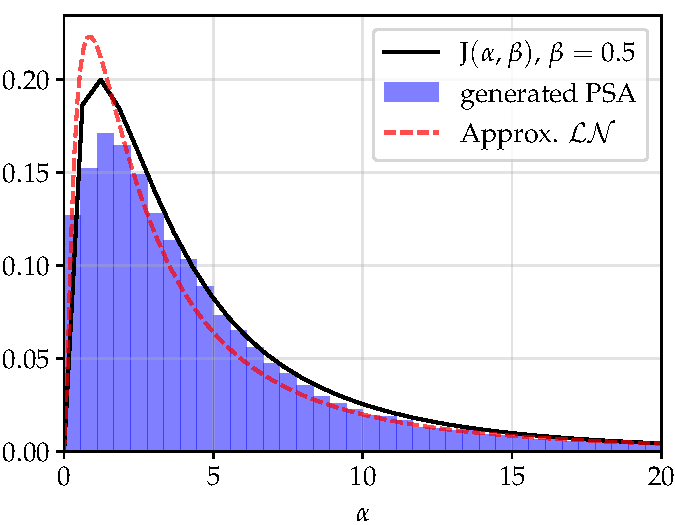
\includegraphics[width=5.2cm]{figures/PREM/PSAjeff.pdf}
        \hspace*{0.5cm}
        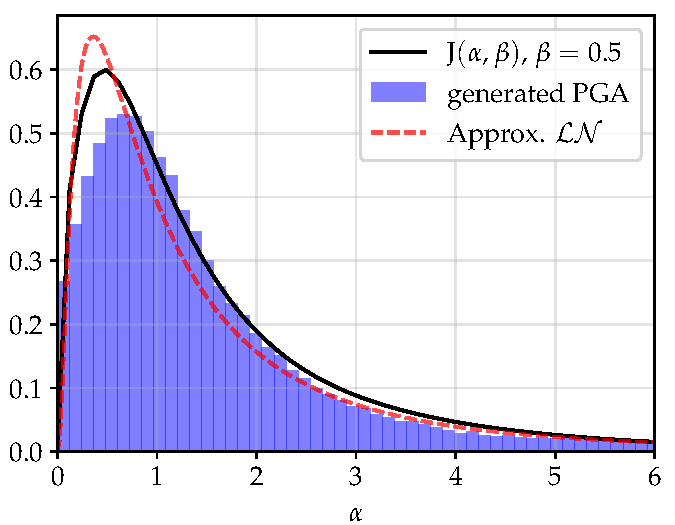
\includegraphics[width=5.2cm]{figures/PREM/PGAjeff.pdf}
        \caption{%
        Comparison of a sectional view of the Jeffreys' prior w.r.t. $\alpha$ (black) with the histograms of the generated signals (blue) and the log-normal approximations (red) for both IMs (PSA in the left figure, PGA in the right figure).
        %Comparison of a sectional view of the Jeffreys prior w.r.t. $\alpha$ (blue line) with some PGA distributions: approximated distribution of real accelerograms via Gaussian kernels in red, histogram of the generated signals in gray, and log-normal fit of the distribution in black.
        }
        \label{fig:IM}
    \end{figure}

    In practice, the use of Markov Chain Monte-Carlo (MCMC) methods (see \cref{sec:PREM:competing}) to sample the \emph{a posteriori} distribution means that the prior must be evaluated (up to a multiplicative constant) many times during the calculations. Considering the computational complexity stemming from the integrals that need to be calculated, it was decided to perform the evaluations of the prior on an experimental design based on a fine-mesh grid of $\Theta$ (here $(0,+\infty)^2$) and to build an interpolated approximation of the Jeffreys prior matching this design. This strategy is more suitable for our numerical applications and very tractable because $\Theta$ is a two-dimensional domain. \Cref{fig:jeff_prior} shows plots of the Jeffreys prior for the two IMs considered. To be precise, $2000\times2000$ prior values were computed for 
    $(\alpha,\beta)\in[10^{-5},50]\times[10^{-5},2]$ in the case of the PSA, and
    $(\alpha,\beta)\in[10^{-5},10]\times[10^{-3},2]$ in the case of the PGA. %and $\alpha\in[]$ and $\beta\in[10^{-3},2]$ and 
    These values are then processed in order to obtain a linear interpolation. 
 
    \begin{figure}[h] %[!ht]
        \centering
        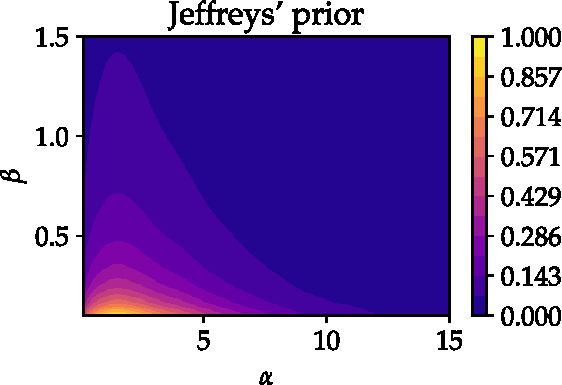
\includegraphics[width=5cm]{figures/PREM/Jeff_prior_PSA-1.pdf}\hspace*{0.5cm}
        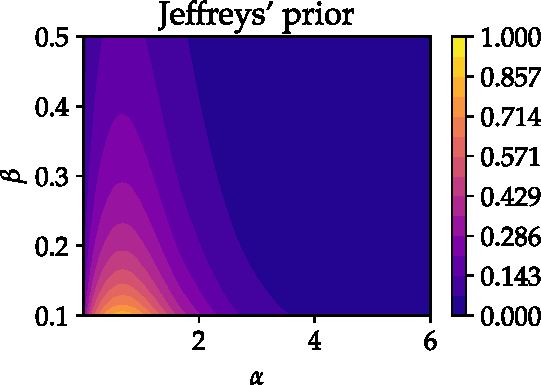
\includegraphics[width=5cm]{figures/PREM/Jeff_prior_PGA-2.pdf}
        %\includegraphics[width=220pt]{figures/Jeffreys_prior.pdf}%\includegraphics[height=0.4\linewidth]{figures/}
        \caption{The Jeffreys' priors calculated from PSA (left) and PGA (right) on subdomains of $\Theta=(0,+\infty)^2$.}
        \label{fig:jeff_prior}
    \end{figure}
    
    %\subsection{Discussion}\label{sec:JeffDiscussion}







    The computational complexity of the Jeffreys prior is not in itself a major drawback. Since it depends exclusively on the distribution of the IM, the initial cost of the Jeffreys prior’s complex calculation would quickly be recovered in installations on the scale of a nuclear power plant, where it is necessary to determine the fragility curves of many Structures and Components (SCs). Compared to methodologies that aim to define a prior based on mechanical calculations which are, by definition, specific to SCs, the generic character of the Jeffreys prior is a clear advantage. This will be explored in the applications section of this paper (Section~\ref{sec:application}). Moreover, the Jeffreys prior is completely defined and does not depend on any additional subjective choices. 
    
    %The Jeffreys prior is known to be improper in numerous common cases (i.e., it cannot be normalized as a probability). This is relevant to our study, as evidenced in \ref{app:asymptotics}, where a calculation of the asymptotic behavior for different limits of $\theta = (\alpha,\beta)$ shows that the Jeffreys prior is indeed improper in our case. However, this characteristic is not an issue since our study focuses on the posterior, which is itself proper, as proven in \ref{app:asymptotics}. This is a critical issue, since MCMC algorithms would not make any sense if the posterior were improper. These asymptotic expansions also provide complementary and essential insight into the Jeffreys prior. They make it possible to understand that its behavior in $\alpha$ is similar to that of a log-normal distribution having the same median as that of the IM (i.e., here 1.1~m/s$^2$) with a variance calculated as the sum of the variance of the IM and of a term that depends on $\beta$. Figure~\ref{fig:IM} clearly illustrates this result.
    



    \subsection{Thorough study of the prior's decay rates}\label{sec:PREM:subsec:jeffasymp}


    Since the Jeffreys prior is known to be often improper, we propose in this section to determine its asymptotic decay rates. In the \cref{sec:PREM:degeneracy}, the decay rates of the likelihood well be computed as well, leading us to elucidate whether the posteriors yielded by Jeffreys are propers.

    We focus on the asymptotic behavior of Jeffreys in four bounds of the space $\Theta$, the study is compiled in the following propositions. 
    The statements rely on the assumption below about the distribution of the IM. %This assumption is the most appropriate 
    The comparison in \cref{fig:IM} illustrates the correctness of this assumption.


    \begin{assu}
        The IM is distributed according to a log-normal distribution, i.e., there exists $\mu\in \RR$ and $\sigma\in (0,+\infty)$ such that 
    \begin{equation}
        p(a) = \frac{1}{\sqrt{2\pi\sigma^2}a}\exp\left({-\frac{(\log a-\mu)^2}{2\sigma^2}}\right).
    \end{equation}
    \end{assu}
    %propositions that are developed below.
    %They are preceded by  the statement of two useful lemmas.

    \begin{prop}\label{prop:jeffb0}
        Fixing $\alpha>0$, there exists a $D'(\alpha)>0$ such that
            \begin{equation}
               J(\theta)\equi{\beta\rightarrow0} \frac{D'(\alpha)}{\beta}.
            \end{equation}
    \end{prop}

    \begin{prop}\label{prop:jeffbinf}
        %    Fix $\alpha>0$, there exists a constant $E'>0$ such that
        {There exists a constant $E'>0$ such that for any $\alpha>0$}
            \begin{equation}
                J(\theta)\equi{\beta\rightarrow\infty}\frac{E'}{\alpha\beta^3}.
            \end{equation}
        \end{prop}
        
        \begin{prop}\label{prop:jeffalph}
            Fixing $\beta>0$, there exists a $G''(\beta)>0$ such that
            \begin{equation}
            J(\theta) \equi{|\log\alpha|\rightarrow\infty} G''(\beta)\frac{|\log\alpha|}{\alpha}\exp\left(-\frac{(\log\alpha-\mu)^2}{2\beta^2+2\sigma^2}\right). 
        \end{equation}
        \end{prop}


    To prove these statements, we rely on the two following lemmas, which provide upper bounds for the function $\gamma\mapsto[\Phi(\gamma)(1-\Phi(\gamma))]^{-1}$.



     \begin{lem}\label{lem:phi(1-phi)ineq1}
        For any $\gamma\in\RR$, $[\Phi(\gamma)(1-\Phi(\gamma))]^{-1}\leq4\exp\left(2\gamma^2/\pi\right)$.
     \end{lem}

     \begin{lem}\label{lem:phi(1-phi)ineq2} For any $\gamma\in\RR$,
        \begin{equation}
        \Phi(\gamma) (1-\Phi(\gamma)) \geq \frac{\sqrt{2/\pi}\exp(-\gamma^2/2)}{  (|\gamma|+\sqrt{\gamma^2+4}) }. 
    \end{equation}
        
    \end{lem}


     \begin{proof}[Proof of \cref{lem:phi(1-phi)ineq1}]
        From the following inequality about the $\erf$ function \citep{chu_bounds_1955}:
\begin{equation}
        \forall \gamma>0,\, \sqrt{1-e^{-\frac{\gamma^2}{2}}}\leq\erf(\gamma/\sqrt{2})\leq\sqrt{1-e^{-2\frac{\gamma^2}{\pi}}},
    \end{equation}
we can deduce that, for any $\gamma>0$,
\begin{equation}
\begin{aligned}
    e^{-\frac{2\gamma^2}{\pi}}\hspace*{-3pt}&\leq 1-\erf(\gamma/\sqrt{2})^2\leq e^{-\frac{\gamma^2}{2}} ,  \\
    \frac{1}{4}e^{-\frac{2\gamma^2}{\pi}}\hspace*{-3pt}&\leq\frac{1}{4}\left(1-\erf\left({\gamma}/{\sqrt{2}}\right)\right)\left(1+\erf\left({\gamma}/{\sqrt{2}}\right)\right)\leq\frac{1}{4} e^{-\frac{\gamma^2}{2}}  , 
\end{aligned}
\end{equation}
the middle term being equal to $\Phi(\gamma)(1-\Phi(\gamma))$. This implies that:
\begin{equation}
    [\Phi(\gamma)(1-\Phi(\gamma))]^{-1}\leq 4 e^{\frac{2\gamma^2}{\pi}} ,
\end{equation}
hence the result for $\gamma>0$.

While it is clear that the inequality still stands for $\gamma=0$, notice that from $\Phi(-\gamma)=1-\Phi(\gamma)\,\forall\gamma\in\RR$ it follows that $\gamma\mapsto\Phi(\gamma)(1-\Phi(\gamma))$ is an even function. Thus, the inequality still stands for any $\gamma<0$; this concludes the proof of the lemma.
     \end{proof}



\begin{proof}[Proof of lemma \ref{lem:phi(1-phi)ineq2}]
    Komatsu's inequality \citep[p.~17]{ito_diffusion_1974}:
    \begin{equation}
        \forall \gamma>0,\, \frac{2}{\sqrt{\gamma^2+4}+\gamma}\leq e^{\frac{\gamma^2}{2}}\hspace*{-4pt}\int_\gamma^\infty\hspace*{-4pt} e^{-\frac{t^2}{2}}dt\leq \frac{2}{\sqrt{\gamma^2+2}+\gamma}
    \end{equation}
    implies
    \begin{equation}
        \forall \gamma>0,\, \frac{2e^{-\frac{\gamma^2}{2}}}{\sqrt{\gamma^2+4}+\gamma}\leq\hspace*{-3.5pt} \sqrt{2\pi}(1-\Phi(\gamma)) \leq\hspace*{-2pt} \frac{2e^{-\frac{\gamma^2}{2}}}{\sqrt{\gamma^2+2}+\gamma} .
    \end{equation}
    Since $0<\Phi<1$ it follows for $\gamma>0$ that:
    \begin{equation}
        \Phi(\gamma)(1-\Phi(\gamma)) \geq \frac{2e^{-\frac{\gamma^2}{2}}}{\sqrt{\gamma^2+4}+\gamma}\left(1-\frac{2e^{-\frac{\gamma^2}{2}}}{\sqrt{\gamma^2+2}+\gamma}\right)
            \geq \frac{\sqrt{2/\pi}e^{-\frac{\gamma^2}{2}}}{\sqrt{\gamma^2+4}+\gamma}.
    \end{equation}
    Finally, since $\Phi(-\gamma)=1-\Phi(\gamma)$, $\gamma\mapsto\Phi(\gamma)(1-\Phi(\gamma))$ is an even function and we obtain for any $\gamma\in\RR$
    \begin{equation}
        \Phi(\gamma)(1-\Phi(\gamma))\geq \frac{\sqrt{2/\pi}e^{-\frac{\gamma^2}{2}}}{\sqrt{\gamma^2+4}+|\gamma|}.
    \end{equation}
\end{proof}






\subsubsection{Proofs of the propositions}
    

\begin{proof}[Proof of \cref{prop:jeffb0}]
    Let $\alpha>0$. For $0\leq k\leq2$, let us consider $A_{k1,k2}=A_{k1}+A_{k2}$ with $A_{kj}$ defined in (\ref{eq:Aij}):
\begin{equation}
    A_{k1,k2} =  \int_{0}^{\infty}\log^k\frac{a}{\alpha}\frac{\Phi'(\gamma(a))^2}{\Phi(\gamma(a))(1-\Phi(\gamma(a)))}h(a)da .
\end{equation}
A substitution gives
    \begin{equation}
        \label{eq:AkAk}
        A_{k1,k2} =   \beta^{k+1}\int_{-\infty}^\infty  F_{A_{k1,k2}}(\gamma)d\gamma , \quad\text{with}\quad
        F_{A_{k1,k2}}(\gamma) =  \frac{\gamma^k}{2\sqrt{\pi^3\sigma^2}} \frac{e^{-\gamma^2}e^{-\frac{(\beta\gamma-\mu+\log\alpha)^2}{2\sigma^2}}}{\Phi(\gamma)(1-\Phi(\gamma))} .
    \end{equation}
%\antoine{
%Let us on another hand state the following useful inequality which we demonstrate later.
%\begin{lem}\label{lem:phiineq}
%    For any $\gamma\in\RR$, $[\Phi(\gamma)(1-\Phi(\gamma)]^{-1}\leq4\exp\left(2\gamma^2/\pi\right)$.
%\end{lem}
%}
%We remind on another hand the following inequality about the $\erf$ function (see \cite{Chu1955}):
%    \begin{equation*}
%        \forall \gamma>0,\, \sqrt{1-e^{-\gamma^2}}\leq\erf(\gamma)\leq\sqrt{1-e^{-4\frac{\gamma^2}{\pi}}}
%    \end{equation*}
%which gives using $\Phi(-\gamma)=1-\Phi(\gamma)$,
    % \begin{equation}\label{eq:Jasymp:Phiineq}
    %     \forall \gamma\in\RR,\, [\Phi(\gamma)(1-\Phi(\gamma))]^{-1}\leq4e^{2\frac{\gamma^2}{\pi}}.
    % \end{equation}
Using \cref{lem:phi(1-phi)ineq1} an upper bound can be derived for $F_{A_{k1,k2}}$: for any $\gamma\in\RR,\,\beta>0$,
\begin{equation}\label{eq:Jasymp:majFkk}
    |F_{A_{k1,k2}}(\gamma)|\leq \tilde C|\gamma|^ke^{-\frac{1}{3}\gamma^2},
\end{equation}
which defines an integrable function on $\RR$, $\tilde C$ being a constant independent of $\gamma$ and $\beta$. Hence the limit
\begin{equation}
    \lim_{\beta\rightarrow0}\int_{-\infty}^\infty F_{A_{k1,k2}}(\gamma)d\gamma =\hspace*{-3pt} \int_{-\infty}^\infty \frac{\gamma^k}{2\sqrt{\pi^3\sigma^2}}\frac{e^{-\gamma^2}e^{-\frac{(\mu-\log\alpha)^2}{2\sigma^2}}}{\Phi(\gamma)(1-\Phi(\gamma))}d\gamma.
\end{equation}
{%
The last integral is null when $k=1$ since the integrand is odd in this case.
When $k$ is even, the integrand is positive valued almost everywhere, which implies that the integral is positive. 
From this, we can establish that  $A_{k1,k2}\equi{\beta\rightarrow0}D_k(\alpha)\beta^{k+1}$ for some $D_k(\alpha)>0$ if $k=0,2$, and $A_{11,12}\aseq{\beta\rightarrow0}o(\beta^2)$.}

Looking back at the Fisher information matrix, we can state that
    \begin{equation}
        \det\cI(\theta)\aseq{\beta\rightarrow0}\frac{D_0(\alpha)D_2(\alpha)}{\alpha^4\beta^2} + o\left(\frac{1}{\beta^2}\right).
    \end{equation}
Finally, we obtain:
\begin{equation}\label{eq:Jrate}
    J(\theta)\equi{\beta\rightarrow0} \frac{D'(\alpha)}{\beta},
\end{equation}
where $D'(\alpha)>0$ is a constant independent of $\beta$.
\end{proof}





\begin{proof}[Proof of proposition \ref{prop:jeffbinf}]

The asymptotic expansion of the $\erf$ function in $0$ is:
    \begin{equation}
        \erf(\gamma)\aseq{\gamma\rightarrow0}\frac{2}{\sqrt{\pi}} \gamma+O(\gamma^2) ,
    \end{equation}
which allows us to state the behavior of $\Phi(\gamma)$ when $\gamma\to0$: 
\begin{equation}
    \Phi(\gamma)\aseq{\gamma\rightarrow0} \frac{1}{2} + \frac{1}{\sqrt{2\pi}} \gamma+O(\gamma^2).    
\end{equation}
 
Let us now fix $\alpha>0$ and consider $A_{k1,k2}= A_{k1}+A_{k2}$ written as:
\begin{equation}
   A_{k1,k2} = \int_{-\infty}^\infty \tilde F_{A_{k1,k2}}(x)dx, \quad\text{with}\quad
    \tilde F_{A_{k1,k2}}(x) = \frac{x^k}{2\sqrt{\pi^3\sigma^2}}\frac{e^{-\frac{x^2}{\beta^2}}e^{-\frac{(x-\mu+\log\alpha)^2}{2\sigma^2}}}{\Phi(\beta^{-1}x)(1-\Phi(\beta^{-1}x))}.
        %&= \int_{0}^{+\infty}F_{A_{k1,k2}}(x)dx + \int_{-\infty}^0F_{A_{k1,k2}}(x)dx \nonumber\\
        %&= A_{k1,k2}^+ + A_{k1,k2}^- \label{eq:binf:splitAk}
\end{equation}
Let us note the convergence of $\tilde F_{A_{k1,k2}}(x)$ towards %$\frac{2x^k}{\sqrt{\pi^3\sigma^2}}e^{-\frac{(x-\mu+\log\alpha)^2}{2\sigma^2}}$ which defines a function in $L^1(\RR)$.
an integrable function when $\beta\to\infty$.
Moreover, \cref{lem:phi(1-phi)ineq1} allows us to bound $\tilde F_{A_{k1,k2}}$:
\begin{equation}
    |\tilde F_{A_{k1,k2}}(x)|\leq \frac{2|x|^k}{\sqrt{\pi^3\sigma^2}}e^{-\frac{(x-\mu+\log\alpha)^2}{2\sigma^2}} e^{2\frac{x^2}{\pi\beta^2}} 
        \leq \frac{2|x|^k}{\sqrt{\pi^3\sigma^2}} e^{-\frac{(x^2-2(\mu-\log\alpha))^2}{4\sigma^2}} e^{\frac{(\mu+\log\alpha)^2}{2\sigma^2}} ,
\end{equation}
for any $x\in\RR$ and $\beta>2\sigma/\sqrt{\pi}$. This dominating function is integrable on $\RR$. Thus, when $\beta\to\infty$, $A_{k1,k2}$ admits a limit expressed by:
\begin{equation}
    \lim_{\beta\rightarrow\infty}A_{k1,k2} = E_k(\alpha) = \int_{-\infty}^\infty\frac{2x^k}{\sqrt{\pi^3\sigma^2}}e^{-\frac{(x-\mu+\log\alpha)^2}{2\sigma^2}} dx= \frac{2\sqrt{2}}{\pi}\EE[X^k] ,
\end{equation}
with $X\sim\cN(\mu-\log\alpha,\sigma^2)$.
Recalling the expression of the Jeffreys prior:
    \begin{equation}
        J(\theta)^2 = \left|\frac{1}{\alpha^2\beta^6}A_{01,02}A_{21,22} - \frac{1}{\alpha^2\beta^6}A_{11,12}^2\right| ,
    \end{equation}
    we can deduce that it is equivalent to $(E_0(\alpha)E_2(\alpha)-E_1^2(\alpha))/\alpha^2\beta^6$ when $\beta\to\infty$.
    Finally,
    \begin{equation}
        J(\theta)\equi{\beta\rightarrow\infty}\frac{E'}{\alpha\beta^3} ,
    \end{equation}
with $E'=\sqrt{E_0(\alpha)E_2(\alpha)-E_1^2(\alpha)} = 2 \sigma /\pi$.

\end{proof}



\begin{proof}[Proof of \cref{prop:jeffalph}]
    
As a preliminary result, let us recall that $\erf(x)\aseq{x\rightarrow\infty}1-\frac{e^{-x^2}}{x\sqrt{\pi}} + o\left(\frac{e^{-x^2}}{x}\right)$, to establish
%use \cref{eq:Jasymp:phiasymp} to obtain
\begin{equation}\label{eq:Jasymp:Phi(1-Phi)equi}
    \Phi(\gamma)(1-\Phi(\gamma))\equi{|\gamma|\to\infty} \frac{e^{\frac{-\gamma^2}{2}}}{|\gamma|\sqrt{2\pi}}.
\end{equation}
% and we remind Komatsu's inequality:
% \begin{equation}\label{eq:komatsu}
%     \Phi(x) (1-\Phi(x)) \geq 1/ [ \sqrt{2\pi} (|x|+\sqrt{x^2+4}) ] \exp(-x^2/2)
% \end{equation}

%and to notice the monotony of $\Phi$ and its property $0<\Phi<1$, which precise the last result with the inequality
%\begin{equation}\label{eq:Jasymp:Phi(1-Phi)ineq}
%    \forall\gamma\in\RR,\, \Phi(\gamma)(1-\Phi(\gamma)) \geq \frac{e^{\frac{-\gamma^2}{2}}}{|\gamma|\sqrt{2\pi}}.
%\end{equation}

Let us consider $A_{k1,k2}=A_{k1}+A_{k2}$:
\begin{equation}
     A_{k1,k2} = C'\int_0^{\infty}\left(\log\frac{a}{\alpha}\right)^k\frac{e^{-\frac{1}{\beta^{2}}\log^2\frac{a}{\alpha}}e^{-\frac{(\log a-\mu)^2}{2\sigma^2}}}{\Phi(\beta^{-1}\log\frac{a}{\alpha})\left(1-\Phi(\beta^{-1}\log\frac{a}{\alpha})\right)}\frac{da}{a},
\end{equation}
denoting $C'=\sqrt{4\pi^3\sigma^2}^{-1}$. By substituting
\begin{equation}
    \nu = \log a - \frac{\sigma^2}{\sigma^2+ \beta^2}\log\alpha - \frac{\beta^2}{\sigma^2+\beta^2}\mu = \log a -r\log\alpha - s\mu,
\end{equation}
we obtain
\begin{equation}%\label{eq:Jasymp:Ak_nu}
     A_{k1,k2} = C'\int_{-\infty}^\infty \hat F_{A_{k1,k1}}(\nu)d\nu , 
\end{equation}
with
\begin{equation}
    \hat F_{A_{k1,k1}}(\nu)=   (\nu+(r-1)\log\alpha +s\mu)^k\frac{e^{-\frac{(\nu + (r+1)\log\alpha +s\mu)^2 }{\beta^2} } e^{-\frac{(\nu +r\log\alpha+ (s-1)\mu)^2}{2\sigma^2}}}{\left[\Phi(1-\Phi)\right](h_\beta(\nu))} ,
\end{equation}
and where $h_\beta(\nu)=\beta^{-1}(\nu+(r-1)\log\alpha+s\mu)$. Using \cref{eq:Jasymp:Phi(1-Phi)equi}, we obtain
\begin{equation}\label{eq:Jasymp:phi1phinurs}
    \left[\Phi(1-\Phi)\right](h_\beta(\nu))\hspace*{-2pt} \equi{|\log\alpha|\rightarrow\infty} \hspace*{-1pt}\frac{\beta e^{-\frac{(\nu+(r-1)\log\alpha+s\mu)^2}{2\beta^2}}}{|\nu + (r-1)\log\alpha + s\mu|\sqrt{2\pi}}.
\end{equation}
Then for a clear understanding of the asymptotic behavior of $\hat F_{A_{k1,k2}}$, let us compute 
\begin{equation}
    \begin{aligned}
        % \nonumber
     -&\frac{(\nu + (r-1)\log\alpha +s\mu)^2 }{2\beta^2} - \frac{(\nu +r\log\alpha+ (s-1)\mu)^2}{2\sigma^2} \\
% \nonumber
=& -\left(\frac{1}{2\beta^2}+\frac{1}{2\sigma^2}\right)\nu^2 -\left(\frac{((r-1)\log\alpha+s\mu)^2}{2\beta^2} +\frac{(r\log\alpha+(s-1)\mu)^2}{2\sigma^2}\right)%\nonumber
\\
         =& -\left(\frac{1}{2\beta^2}+\frac{1}{2\sigma^2}\right)\nu^2 - \frac{(\log\alpha - \mu )^2}{2(\beta^2+\sigma^2)}.
\label{eq:Jasymp:nurs}
    \end{aligned}
\end{equation}
We expand $\hat F_{k1,k2}(\nu) = \sum_{j=1}^kC_k^j(r-1)^j\log^j\alpha(\nu+s\mu)^{k-j}g(\nu)$ $ = \sum_{j=0}^k\hat F_{k1,k2}^{(j)}(\nu)$, with $g(\nu)$ defined as    \begin{equation*}
        g(\nu) = \frac{e^{-\frac{(\nu + (r+1)\log\alpha +s\mu)^2 }{\beta^2} } e^{-\frac{(\nu +r\log\alpha+ (s-1)\mu)^2}{2\sigma^2}}}{\left[\Phi(1-\Phi)\right](\beta^{-1}(\nu + (r-1)\log\alpha + s\mu))}.
    \end{equation*}
Therefore, by combining \cref{eq:Jasymp:phi1phinurs,eq:Jasymp:nurs}, we obtain that $\hat F_{k1,k2}^{(j)}$ satisfies
    \begin{equation}
         \hat F_{k1,k2}^{(j)}(\nu)e^{\frac{(\log\alpha-\mu)^2}{2\beta^2+2\sigma^2}}(\log\alpha)^{-j}|\log\alpha|^{-1} 
            \conv{|\log\alpha|\rightarrow\infty} (\sqrt{2\pi}\beta)^{-1}C_k^j(r-1)^{j+1}(\nu+s\mu)^{k-j} e^{-\left(\frac{1}{2\beta^2}+\frac{1}{2\sigma^2}\right)\nu^2}.
    \end{equation}
Using \cref{lem:phi(1-phi)ineq2}, we can also define an integrable upper bound for the above function as: %in the form of an integrable function expressed as
\begin{equation}
    |\hat F_{k1,k2}^{(j)}(\nu)|e^{\frac{(\log\alpha-\mu)^2}{2\beta^2+2\sigma^2}}|\log\alpha|^{-j-1} \leq \frac{\sqrt{2/\pi}e^{-\left(\frac{1}{2\beta^2}+\frac{1}{2\sigma^2}\right)\nu^2}}{ |h_\beta(\nu)|+\sqrt{h_\beta(\nu)^2+4}} \leq\frac{1}{\sqrt{2\pi}}e^{-\left(\frac{1}{2\beta^2}+\frac{1}{2\sigma^2}\right)\nu^2}.
\end{equation}
Thus, we can switch the limits and the integration, and the following results are obtained:
\begin{align}
    C''\beta A_{01,02}e^{\frac{(\log\alpha-\mu)^2}{2\beta^2+2\sigma^2}} &\aseq{\log\alpha\rightarrow\infty} (1-r)G\log\alpha - s\mu G  +o(1)\\
    C''\beta A_{11,12}e^{\frac{(\log\alpha-\mu)^2}{2\beta^2+2\sigma^2}}
        &\aseq{\log\alpha\rightarrow\infty} -(1-r)^2G\log^2\alpha - s^2\mu^2 G 
        + 2(1-r)s\mu G\log\alpha - G' + o(1),\\
%\end{align}
%\begin{align}
C''\beta A_{22,22}e^{\frac{(\log\alpha-\mu)^2}{2\beta^2+2\sigma^2}}
&\aseq{\log\alpha\rightarrow\infty}\hspace*{-4pt}
(1-r)^3G\log^3\alpha - s^3\mu^3 G 
-3(1-r)^2s\mu G\log^2\alpha \\
&\hspace*{2em}-3(1-r)s^2\mu^2 G\log\alpha+3(1-r)G'\log\alpha  + o(1), \nonumber
\end{align}
%
% \begin{align*}
%     C''\beta A_{01,02}e^{\frac{(\log\alpha-\mu)^2}{2\beta^2+2\sigma^2}} \aseq{\log\alpha\rightarrow\infty}& (1-r)G\log\alpha - s\mu G  +o(1)\\
%     C''\beta A_{11,12}e^{\frac{(\log\alpha-\mu)^2}{2\beta^2+2\sigma^2}} \aseq{\log\alpha\rightarrow\infty} & -(1-r)^2G\log^2\alpha - s^2\mu^2 G + 2(1-r)s\mu G\log\alpha - G' + o(1)\\
%     C''\beta A_{22,22}e^{\frac{(\log\alpha-\mu)^2}{2\beta^2+2\sigma^2}} \aseq{\log\alpha\rightarrow\infty} & (1-r)^3G\log^3\alpha - s^3\mu^3 G -3(1-r)^2s\mu G\log^2\alpha \\
%         &+3(1-r)s^2\mu^2 G\log\alpha +3(1-r)G'\log\alpha  + o(1)
% \end{align*}
with $C''=(C'\sqrt{2\pi})^{-1}$, $G=\sigma\beta\sqrt{2\pi(\beta^2+\sigma^2)^{-1}}$ and $G'=G^2/2\pi$. 
This way
\begin{align}\nonumber
    C''\alpha\beta^{8} J(\theta)^2e^{\frac{(\log\alpha-\mu)^2}{2\beta^2+2\sigma^2}}
      &  \aseq{\log\alpha\rightarrow\infty}\hspace*{-4pt}  
        3(r-1)^2s^2\mu^2G^2\log^2\alpha 
        + 3(r-1)^2s^2\mu^2G^2\log^2\alpha \\
        &\hspace*{2em} +3 (r-1)^2GG'\log^2\alpha 
        - 4(r-1)^2s^2\mu^2G^2\log^2\alpha \\
        &\hspace*{2em} - 2(r-1)^2s^2\mu^2G^2\log^2\alpha - 2(r-1)^2GG'\log^2\alpha %\\
        % &\hspace*{2em}
        + o(\log^2\alpha).\nonumber
\end{align}
Note that the above equality is still valid when $\log\alpha\to-\infty$. Finally,
\begin{equation}
    J(\theta) \equi{|\log\alpha|\rightarrow\infty} G''(\beta)\frac{|\log\alpha|}{\alpha}\exp\left(-\frac{(\log\alpha-\mu)^2}{2\beta^2+2\sigma^2}\right)  ,
\end{equation}
with 
\begin{align}
    G''(\beta) &=C''^{-1}(r-1)^2GG'\beta^{-4} 
        = \frac{2\sigma^3\beta^3 }{\sqrt{\pi}(\sigma^2+\beta^2)^{7/2}}. %\frac{\sigma^3\beta^3\sqrt{2\pi}^3}{\sqrt{\beta^2 + \sigma^2}^32\pi}\beta^{-4} .
\end{align}


\end{proof}

\section{Competing approaches and estimation tools}\label{sec:PREM:competing}



    \subsection{Bayesian estimates of the seismic fragility curve}


    The most relevant method in order to benefit from the Bayesian theory and the reference prior construction presented in \cref{sec:PREM:model} consists in deriving the posterior defined in \cref{eq:PREM:posterior}.
    When the latter is proper, it then becomes possible to generate, according to that distribution, samples of $\theta$ conditioned on the observed data. These \emph{a posteriori} generations of $\theta$ can be obtained using MCMC methods. In this study, we have implemented an adaptive Metropolis-Hastings (M-H) algorithm with a Gaussian transition kernel and a covariance adaptation process (following the suggestions of \cite{haario_adaptive_2001}). Such an algorithm allows sampling from a probability density known up to a multiplicative constant. In this context, the \emph{a posteriori} samples of $\theta$ can be used to define credibility intervals for the log-normal estimations of the fragility curves.



    \subsection{Competing prior taken from the literature}

    {For comparison purposes, we selected the prior} suggested by \citet{straub_improved_2008} ---called the SK prior--- whose density is defined as the product of a normal distribution for $\ln(\alpha)$ and the improper distribution $1/\beta$ for $\beta$, namely:
    \begin{equation}\label{eq:Straubprior}
        \pi_{SK}(\theta)\propto\frac{1}{\alpha\beta} \exp\Big( -\frac{(\log\alpha-\mu)^2}{2\sigma^2}\Big).
    \end{equation}
In \cite{straub_improved_2008}, the parameters $\mu$ and $\sigma$ of the log-normal distribution are chosen to generate a non-informative prior. 
%As specified in the introduction to Section~\ref{sec:tools}, 
For a fair comparison with the approach proposed in this paper, we decided to pick $\mu$ and $\sigma$ as equal to the mean and the standard deviation of the logarithm of the IM. This choice is consistent with the fact that the Jeffreys prior is similar to a log-normal distribution with these parameters (see \cref{fig:IM}). The prior $\pi_{SK}(\theta)$ is plotted in \cref{fig:Straubprior} for both the PSA and the PGA as IM.

\begin{figure}[h]
    \centering
    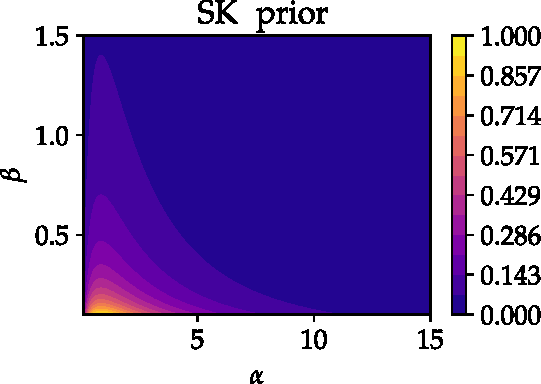
\includegraphics[width=5cm]{figures/PREM/SK_prior_PSA.pdf}\hspace*{0.5cm}
    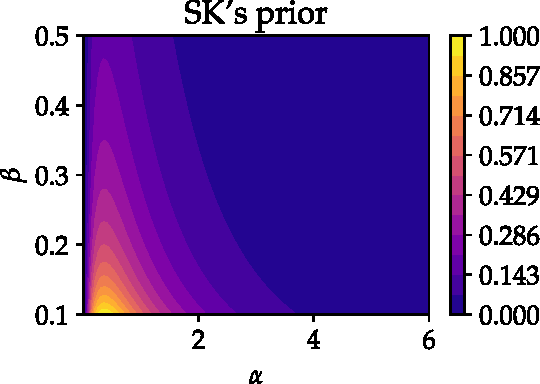
\includegraphics[width=5cm]{figures/PREM/SK_prior_PGA.pdf}
    %\includegraphics[width=210pt]{figures/SK.pdf} %height=0.4\linewidth
    \caption{Prior suggested by \citet{straub_improved_2008},  expressed in \cref{eq:Straubprior} and scaled to a log-normal estimation of the IM distribution, for both the PSA (left) and the PSA (right) as IM.}
    \label{fig:Straubprior}
\end{figure}


An analysis of the posterior obtained from the SK prior is given in \cref{sec:PREM:degeneracy}. It shows that the posterior is always improper, which jeopardizes the validity of any \emph{a posteriori} estimation using MCMC methods. This could however be mitigated by truncating w.r.t. $\beta$, which we will do in the numerical application conducted in this work. This issue persists in the authors' original framework, which is slightly different from ours. This is confirmed in the appendix~\ref{app:SKreview}.


\paragraph{Asymptotic comparison of the Jeffrey and SK priors} 
By comparing the Jeffreys and SK prior asymptotics, it can be observed that:
    \begin{itemize}
        \item Regarding the asymptotics w.r.t. $\beta$, while the divergence rates are the same when $\beta\to0$, the Jeffreys prior performs better when $\beta\to\infty$:
            \begin{equation}
                J(\theta) \underset{\beta\rightarrow\infty}{\propto} \beta^{-2}\pi_{SK}(\theta).
            \end{equation}
        Consequently, the SK posterior will result in higher probabilities for high values of $\beta$ compared to the Jeffreys prior.
        \item Regarding the asymptotics w.r.t. $\alpha$, both are asymptotically close to a log-normal distribution, with a slight ``disadvantage'' for the Jeffreys prior, for which the asymptotic variance is derived by adding $\beta^2$ to the variance of the SK prior. This means that while for small values of $\beta$ (smaller than $\sigma$), both priors remain comparable w.r.t. $\alpha$, the Jeffreys prior gives higher probabilities to $\alpha$ outliers when $\beta$ also has a high value. However, as seen above, the probability for large values of $\beta$ is quite low for the Jeffreys prior compared to the SK prior. %This explains why the generation of such $\alpha$ outliers has not been observed in the estimations presented in this paper.
    \end{itemize}


% \paragraph{}
%


    \subsection{Maximum likelihood estimation with bootstrapping}

The most common non-Bayesian estimator of the seismic fragility curves under the probit-lognormal modeling is the maximum likelihood estimator (MLE). This estimator has been introduced in the \cref{chap:frags-intro} (\cref{sec:intro-frags:models}). It is expressed as follows for the given of observations $(\mbf z^k,\mbf a^k)$:
    \begin{equation}
        \theta^{\text{MLE}}(\mbf z^k,\mbf a^k)=\argmax_{\theta\in\Theta}\ell_k(\mbf z^k|\mbf a^k,\theta).
    \end{equation}
    %$\theta^{\text{MLE}}(\mbf z^k,\mbf a^k)=\argmax_{\theta\in\Theta}\ell_k(\mbf z^k,\mbf a^k|\theta)$.
It is common to compute multiple MLE in order to obtain confidence intervals. Doing so, the bootstrap technique defines the stochastic estimator of $\theta$:
    \begin{equation}
        \hat\theta_k^{\text{BMLE}}(\mbf z^k,\mbf a^k) = \theta^{\text{MLE}}((z_{U_i},a_{U_i})_{i=1}^k),
    \end{equation}    
  where $U_1,\dots,U_k$ are i.i.d. random variables distributed w.r.t. a uniform distribution in $\{1,\dots,k\}$.
This estimator is used to compute confidence intervals by estimating empirically its quantiles from many samples. 
This is a very common approach for fragility curves (e.g., 
\cite{shinozuka_statistical_2000,gehl_influence_2015,baker_efficient_2015}). The convergence of the MLE and the relevance of this method are detailed in \cite{van_der_vaart_asymptotic_1992}. However, the relevance of the bootstrap method is often limited by the irregularity of its results for small values of $k$ (see e.g., \cite{zentner_fragility_2017}).





\section{Limits of the estimates given by the three approaches: the curse of degeneracy}\label{sec:PREM:degeneracy}

In this section, we study the likelihood decay rates in order to (i) explain irregular phenomena commonly encountered with classical frequentist methods, and (ii) verify the proper characteristics of the posteriors in the Bayesian framework.
Our study of the likelihood's asymptotic behavior is summarized in the following proposition.

\begin{prop}\label{prop:likelihood}
    Let us consider $k>1$ and a data sample $(\mbf a^k, \mbf z^k)$. 
    Let us introduce the vectors $\mbf N=(z_i\indic_{a_i<\alpha}+(1-z_i)\indic_{a_i>\alpha})_{i=1}^k$, $\log^2\frac{\mbf a^k}{\alpha}=(\log^2\frac{a_i}{\alpha})_{i=1}^k$.  
    
    \begin{itemize}
        \item Fixing $\alpha>0$, then 
        \begin{equation}
        \ell_k(\mbf z^k|\mbf a^k,\theta) \conv{\beta\rightarrow\infty}2^{-k}\quad\text{and}\quad
        % \end{equation}
% and
        % \begin{equation}
            \ell_k(\mbf z^k|\mbf a^k,\theta) \aseq{\beta\rightarrow0}O\left(\beta^{|\mbf N|}e^{-\frac{\mbf N^T\log^2\frac{\mbf a^k}{\alpha}}{2\beta^2}}\right) ,
        \end{equation}
        where $|\mbf N|=\sum_{i=1}^kN_i$.
        \item Fixing $\beta>0$, then
        \begin{equation}
            \ell_k(\mbf z^k|\mbf a^k,\theta) \hspace*{-3pt} \aseq{\alpha\rightarrow0}\hspace*{-3pt} O\left(|\log\alpha|^{|\mbf z^k|-k} e^{-\frac{1}{2\beta^2}\sum_{i=1}^k (1-z_i)(\log a_i-\log\alpha)^2} \right)
        \end{equation}
        and 
        \begin{equation}
            \ell_k(\mbf z^k|\mbf a^k,\theta) \hspace*{-3pt}\aseq{\alpha\rightarrow\infty}\hspace*{-3pt} O\left(\log(\alpha)^{-|\mbf z^k|} e^{-\frac{1}{2\beta^2}\sum_{i=1}^k z_i(\log a_i-\log\alpha)^2} \right) ,
        \end{equation}
        where $|\mbf z^k|=\sum_{i=1}^kz_i$ is the number of failures in the observed sample.
    \end{itemize}
\end{prop}



\begin{proof}[Proof of \cref{prop:likelihood}]
    As a reminder, the likelihood is expressed as:
    \begin{equation}
    \begin{aligned}%\label{eq:likelitocalc}
        \ell_k(\mbf z^k|\mbf a^k,\theta)  &= \prod_{i=1}^k\Phi\left(\frac{\log a_i-\log\alpha}{\beta}\right)^{z_i}\left(1-\Phi\left(\frac{\log a_i-\log\alpha}{\beta}\right)\right)^{1-z_i} \\
%            & = \prod_{i=1}^k\Phi(\gamma_i)^{z_i}(1-\Phi(\gamma_i))^{1-z_i}\\
            & = \exp\left[\sum_{i=1}^k\left(z_i\log\Phi(\gamma_i) + (1-z_i)\log(1-\Phi(\gamma_i))\right)\right] ,
    \end{aligned}
\end{equation}
denoting $\gamma_i=\beta^{-1}\log\frac{a_i}{\alpha}$. %\antoine{We want to study the bahavior of this expression when the $\gamma_i\to\infty$.} %, note that $\gamma\conv{\beta\rightarrow0}\eps_i\infty$ a.s. where $\eps_i=1$ if $a_i>\alpha$;  \antoine{$-1$ if $a_i<\alpha$; and $0$ otherwise.}

To treat the case where $\beta\to\infty$ we can observe that while $\alpha$ is fixed, the quantities $\Phi(\gamma_i)$ all converge to ${1}/{2}$. The product of those limits gives the limit $\ell_k(\mbf z^k|\mbf a^k,\theta)\conv{\beta\rightarrow\infty}2^{-k}$.


For the other cases, it should be reminded that $\Phi(x)=\frac{1}{2}(1+\erf(x/\sqrt{2}))$ and $\erf(x)\aseq{x\rightarrow\infty}1-\frac{e^{-x^2}}{x\sqrt{\pi}} + o\left(\frac{e^{-x^2}}{x}\right)$, which leads to 
    \begin{equation}\label{eq:Jasymp:phiasymp}
        \Phi(x)\aseq{x\rightarrow\infty}1 - \frac{e^{-\frac{x^2}{2}}}{x\sqrt{2\pi}} + o\left(\frac{e^{-\frac{x^2}{2}}}{x}\right).
    \end{equation}
Let us consider an $i\in\{1,\dots,k\}$ and compute
\begin{equation}
    \begin{aligned}
        &z_i\log\Phi(\gamma_i) + (1-z_i)\log(1-\Phi(\gamma_i)) \\
           &\qquad  \aseq{\gamma_i\rightarrow\infty} z_i\log\left(1-\frac{e^{-\frac{\gamma_i^2}{2}}}{\gamma_i\sqrt{2\pi}} + o\left(\frac{e^{-\frac{\gamma_i^2}{2}}}{\gamma_i}\right)\right)
        %   &\hspace*{2em}
          +(1-z_i)\log\left(\frac{e^{-\frac{\gamma_i^2}{2}}}{\gamma_i\sqrt{2\pi}} + o\left(\frac{e^{-\frac{\gamma_i^2}{2}}}{\gamma_i}\right)\right)\\
           &\qquad \aseq{\gamma_i\rightarrow\infty} -z_i\frac{e^{-\frac{\gamma_i^2}{2}}}{\gamma_i\sqrt{2\pi}}  %o\left(\frac{e^{-\gamma_i^2}}{\gamma_i}\right) 
                +(1-z_i)\log\left(\frac{e^{-\frac{\gamma_i^2}{2}}}{\gamma_i\sqrt{2\pi}}\right) + o(1)\\
           &\qquad \aseq{\gamma_i\rightarrow\infty} - (1-z_i)\frac{\gamma_i^2}{2} - (1-z_i)\log(\gamma_i\sqrt{2\pi}) + o(1).
    \end{aligned}
\end{equation}
Using the relation $\Phi(-x)=1-\Phi(x)$, it follows that, in the case $a_i<\alpha$:
    \begin{equation}
        z_i\log\Phi(\gamma_i) + (1-z_i)\log(1-\Phi(\gamma_i))
            \aseq{\gamma_i\rightarrow-\infty} - z_i\frac{\gamma_i^2}{2} - z_i\log(-\gamma_i\sqrt{2\pi}) + o(1).
    \end{equation}

{
Going back to the likelihood asymptotics, let us first suppose $\alpha>0$ and $\beta\to0$. Thus, denoting the vectors $\mbf N=(z_i\indic_{a_i<\alpha}+(1-z_i)\indic_{a_i>\alpha})_{i=1}^k$ and 
$\log^2\frac{\mbf a^k}{\alpha}=(\log^2\frac{a_i}{\alpha})_{i=1}^k$, we obtain
    \begin{equation}
        \ell_k(\mbf z^k|\mbf a^,\theta) \aseq{\beta\rightarrow0} \frac{C(\alpha)}{\sqrt{2\pi}^{|\mbf N|}}\beta^{|\mbf N|} e^{-\frac{\mbf N^T\log^2\frac{\mbf a^k}{\alpha}}{2\beta^2}+o(1)} %\mbox{ is a constant}
            \aseq{\beta\rightarrow0}O\left(\beta^{|\mbf N|}e^{-\frac{\mbf N^T\log^2\frac{\mbf a^k}{\alpha}}{2\beta^2}}\right) ,
    \end{equation}
where $|\mbf N|=\sum_{i=1}^kN_i$ and $C(\alpha) =\prod_{i=1}^k\left|\log\frac{a_i}{\alpha}\right|^{N_i}$. %Note that $N$

Let us then fix $\beta>0$ to get
\begin{equation}
    \begin{aligned}
        \ell_k(\mbf z^k|\mbf a^k,\theta) &\aseq{\alpha\rightarrow\infty} \frac{\beta^{|\mbf N|}}{\sqrt{2\pi}^{|\mbf N|}} \left(\prod_{i=1}^k\log\left(\frac\alpha{a_i}\right)^{-z_i}\right) 
        % &\hspace*{1.5em}\cdot 
        \exp\left({-\frac{1}{2\beta^2}\sum_{i=1}^k z_i(\log a_i-\log\alpha)^2+o(1)}\right)
        \\
            &\aseq{\alpha\rightarrow\infty}O\left(\log(\alpha)^{-|\mbf z^k|} e^{-\frac{1}{2\beta^2}\sum_{i=1}^k z_i(\log a_i-\log\alpha)^2} \right),
    \end{aligned}
\end{equation}
where $|\mbf z^k|=\sum_{i=1}^kz_i$ is the number of failures in the observed sample.
Similarly, we obtain
\begin{equation}
    \begin{aligned}
        \ell_k(\mbf z^k|\mbf a^k,\theta) 
        &\aseq{\alpha\rightarrow0}
            \frac{\beta^{|\mbf N|}}{\sqrt{2\pi}^{|\mbf N|}} \left(\prod_{i=1}^k\log\left(\frac{a_i}\alpha\right)^{-(1-z_i)}\right) 
            % &\hspace*{1.5em}\cdot 
            \exp\left({-\frac{1}{2\beta^2}\sum_{i=1}^k (1-z_i)(\log a_i-\log\alpha)^2+o(1)}\right)
        \\
            &\aseq{\alpha\rightarrow0}O\left(|\log\alpha|^{|\mbf z^k|-k} e^{-\frac{1}{2\beta^2}\sum_{i=1}^k (1-z_i)(\log a_i-\log\alpha)^2} \right).
    \end{aligned}
\end{equation}
}
\end{proof}


This statement expresses that, under general circumstances, the likelihood converges rapidly to $0$ in every direction but the one where $\beta\to\infty$.
The latter is a concern, because it requires that the decay rate of the prior in that direction is proper to yield proper posteriors.
Moreover, under some circumstances, %several problemtaic pheno
the vector $\mbf N$ is null. It is the case when we fall in one the three scenarios described in the following definition.
In that case, we say that the likelihood is degenerate, and it does not converge towards $0$ when $\beta\to0$. 


\begin{defi}[Likelihood degeneracy]\label{def:degeneracy}
    %If the observed data $(\mbf z^k,\mbf a^k)$ are such that, either,
    {If the observed samples $(\mbf z^k,\mbf a^k)$ belong to one of the following three types:}
    \begin{itemize}
        \item {type 1 : no failure is observed: $z_i=0$ for any $i$;}
        \item {type 2 : only failures are observed: $z_i=1$ for any $i$;}
        \item {type 3 : the failures and non-failures are partitioned into two disjoint subsets when classified according to their IM values:}
        %the failures and successes are discriminated according to their IM: 
        there exists $a\in\cA$ such that for any $i,j$, $a_i<a<a_j\Longleftrightarrow z_i\ne z_j$ (see the illustration in \cref{fig:degenerate-frag});
    \end{itemize}
    then the likelihood is degenerate.
\end{defi}



An example of degenerate likelihood is presented in \cref{fig:degenerate-frag} with an illustration of this phenomenon.
In the following, we deduce from this study the decay rates of the posterior densities 
yielded by the two prior considered in this work (the SK prior and the Jeffreys prior).
In particular, we show that the Jeffreys prior may produce improper posteriors in degenerate scenarios.
For this reason, this chapter addresses the estimation of seismic fragility curves from dataset issuing non-degenerate likelihoods.


\begin{figure}
    \centering
    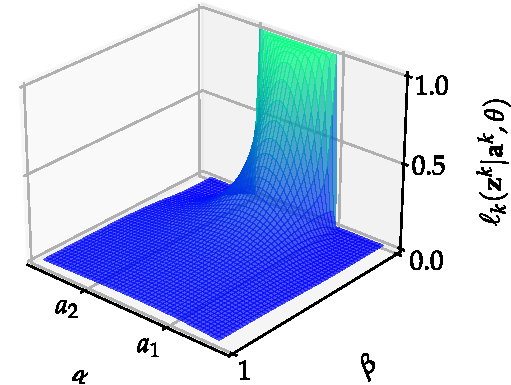
\includegraphics[width=4.6cm]{figures/PREM/likelihood_degen.pdf}\qquad
    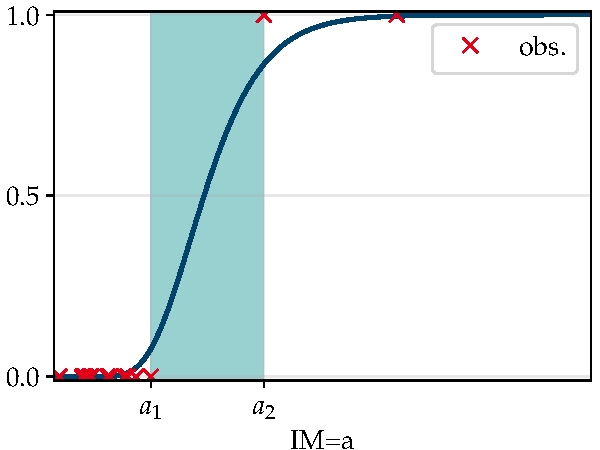
\includegraphics[width=4.44cm]{figures/PREM/degeneracy.pdf}
    \caption{{Example of a type 3 data sample $(\mbf z^k,\mbf a^k)$ which gives a degenerate likelihood. Graphs of (left) the likelihood given the degenerate data sample as a function of the tuple $(\alpha,\beta)$ and (right) the fragility curve (blue curve) according to which the points (red crosses) are sampled : each red cross is a tuple $(z,a)$, where its X-axis equals $a$ and its Y-axis equals $z$.}
    On both figures, $a_1$ is the maximal observed IM value among ``non-failures'', and $a_2$ is minimal one among ``failures''.}
    \label{fig:degenerate-frag}
\end{figure}



%limits the study to case studies where 

\subsubsection{Decay rates of the posterior densities and properness}


The Jeffreys and SK priors are not proper with respect to $\beta$ (see \cref{sec:PREM:Jeffreys} for the Jeffreys prior and eq?? for the SK prior). For the Jeffreys prior, the divergence and convergence rates with respect to $\beta$ only make the resulting posterior proper when the prior is coupled with non-degenerate likelihoods. 
%The particular circumstances leading to a likelihood divergence when $\beta\rightarrow0$, as mentioned in \ref{app:lieklihood-asympt}, do not apply.
 However, one can see that this is not the case for the SK posterior, which is not integrable w.r.t. $\beta$ because of a convergence rate that is too low at $+\infty$. This prevents the validation of the MCMC estimates for this posterior, unless a truncation of the distribution is considered. %This explains the generation of \emph{a posteriori} outliers using the SK prior. 
 Note that \citet{straub_improved_2008} considered this prior within a Bayesian framework that slightly differs from ours. In the appendix~\ref{app:SKreview}, we confirm that the posterior is not proper even when derived in the exact framework of their paper. % \cite{Straub2008}.



% \subsection{Improperness of the SK posterior in the original framework of the authors}



% We stated above that, within our framework, the SK prior always results in an improper posterior. This puts the validity of the MCMC estimations into question, unless if the domain is truncated in $\beta$. %and could explain the lower performance of the SK prior compared to the Jeffreys prior. 
% In \cite{straub_improved_2008}, the authors use the Bayesian methodology the same way we do, yet the consideration of uncertainties over the observed earthquake intensity measures and the equipment capacities leads to a slightly different likelihood.
% In order to verify that the drawbacks of their prior highlighted in this paper are not due to our statistical choices, we dedicated this appendix to the study of the asymptotic expansions of the posterior in the exact framework presented in \cite{Straub2008}.
% We shall first introduce the exact model of \citeauthor{Straub2008} for the estimation of seismic fragility curves in \ref{subapp:C1}, using notations consistent with our study. We will then derive the likelihood and its asymptotics in \ref{subapp:C2}. Finally, we will express the convergence rates of the posterior in \ref{subapp:C3}, which will allow us to conclude that the SK posterior is indeed improper.





\section{Performance evaluation metrics}\label{sec:PREM:metrics}

In order to assess and compare the performances of the proposed approaches, we propose different quantitative metrics.
Beforehand, we suppose we have access to a reference fragility curve $P^{\text{ref}}_f$. In two of the case studies that we treat in the following, a large validation dataset is available and can be used to derive such reference using non-parametric Monte-Carlo estimates following the suggestion of \citet{trevlopoulos_parametric_2019}. This method was described in the \cref{chap:frags-intro} (\cref{sec:intro-frags:models}) and implemented in the \cref{chap:frags-intro} onto two case studies for which a large validation dataset was available.
%We recall briefly the construction of this reference from the validation dataset denoted $(z_i,a_i)_{i=1}^{}$.
% It follows the suggestion of \citet{trevlopoulos_parametric_2019}

Given observations $(\mbf z^k,\mbf a^k)$, we denote by $a\mapsto P_f^{|\mbf z^k,\mbf a^k}(a)$ the random process defined as the fragility curve conditional to the $(\mbf z^k,\mbf a^k)$. Its distribution inherits from the posterior distribution of $\theta$ in the case of the Bayesian method, or it inherits from the distribution of the bootstrap estimator $\hat\theta^{\text{BMLE}}(\mbf z^k,\mbf a^k)$ in the case of the MLE.
For each value $a$, the $r$-quantile of the random variable $P_f^{|\mbf z^k,\mbf a^k}(a)$ is denoted by $q_r^{|\mbf z^k,\mbf a^k}(a)$. We then define:
\begin{itemize}
    \item The quadratic error: $\cE^{|\mbf z^k,\mbf a^k}=\EE_{\theta|\mbf z^k,\mbf a^k}\left[\|P_f^{|\mbf z^k,\mbf a^k}-P_f^{\mathrm{ref}} \|^2_{L^2}\right].$
        \item The $1-r$ square credibility width: $\cW^{|\mbf z^k,\mbf a^k}= \|q_{1-{r/2}}^{|\mbf z^k,\mbf a^k} - q_{{r/2}}^{|\mbf z^k,\mbf a^k}\|_{L^2}^2$.
\end{itemize}
The $L^2$ norm is taken on the domain $[a_{\text{min}},a_{\text{max}}]$ that covers  the available seismic signals: 
\begin{equation}
    \|P\|^2_{L^2} = \int_{a_{\text{min}}}^{a_{\text{max}}} P(a)^2da.    
\end{equation}
The $L^2$ norms are approximated using Simpson's interpolation, and the expectation are estimated by Monte-Carlo sums, using samples following either the posterior distributions or the distribution of the bootstrap estimator. 









\section{Numerical applications}


In this section, we will examine three case studies.
Two of them leverage the many simulation datasets available that have been previously computed for validation purposes. They will be used in the derivation of a reference fragility curve (as explained in \cref{sec:PREM:metrics}), and allow us to validate the corresponding log-normal models. The first case, described in Section~\ref{sec:onl}, deals with a nonlinear oscillator,
for which $N_s=10^5$ nonlinear simulations have been implemented for validation purposes. The second case study, described in Section~\ref{sec:ASG}, deals with a piping system which is part of the secondary cooling system of a French Pressurized Water Reactor. Due to the high computational cost, only $N_s=10^4$ simulations have been performed for this case. In both cases, estimations are performed using different testing data sets of a size $k$ chosen as negligible compared to $N_s$. These testing data sets are taken from the set of available nonlinear dynamical simulation results. {A third case study is presented in ?? %as supplementary material 
in order to showcase how our method could be applied to practical experiments.}




\subsection{Case study 1: the elasto-plastic oscillator}

1

\subsection{Case study 2: the piping system from a pressurized reactor}

\subsection{Case study 3: the stacked structure for storage of packages}


\section{Appendix: a review of the properties of the SK posterior}\label{app:SKreview}



In this paper, we have compared our approach with the one that results from an adaptation of the prior suggested by \citet{straub_improved_2008}. We proved in \cref{sec:PREM:degeneracy} that within our framework, this prior results in an improper posterior. This puts the validity of the MCMC estimations into question, and could explain the lower performance of the SK prior compared to the Jeffreys prior. 
In \cite{straub_improved_2008}, the authors use the Bayesian methodology the same way we do, yet the consideration of uncertainties over the observed earthquake intensity measures and the equipment capacities leads to a slightly different likelihood.
In order to verify that the drawbacks of their prior highlighted in this paper are not due to our statistical choices, we dedicated this appendix to the study of the asymptotic expansions of the posterior in the exact framework presented in \cite{straub_improved_2008}.
We shall first introduce the exact model of their paper for the estimation of seismic fragility curves in \ref{subapp:C1}, using notations consistent with our study. We will then derive the likelihood and its asymptotics in \ref{subapp:C2}. Finally, we will express the convergence rates of the posterior in \ref{subapp:C3}, which will allow us to conclude that the SK posterior is indeed improper.

\subsection{Statistical model and likelihood}
\label{subapp:C1}
Let us consider the observations of earthquakes labeled $l=1,\dots,L$ at equipment labeled $i=1,\dots,I_j$ located in substations labeled $j=1,\dots,J$.
The observed items are $(\mbf z_{jl},\hat a_{jl})_{j,l}$, $\mbf z_{jl}=(z_{ijl})_i$ being the failure occurrences of the $I_j$ pieces of equipment at substation $j$ during earthquake $l$ ($z_{ijl}\in\{0,1\}$), and $\hat a_{jl}$ being the observed IM at substation $j$ during earthquake $l$ ($\hat a_{jl}\in(0,+\infty)$).
They are assumed to follow the latent model presented below.

At substation $j$ the $l$-th earthquake results in an IM value $a_{jl}$ that is observed with an uncertainty multiplicative noise: $\log\hat a_{jl}=\log a_{jl}+\eps_{jl}$ where $\eps_{jl}\sim\cN(0,\sigma_\eps^2)$. The noise variance $\sigma_\eps^2$ is supposed to be known. %, and so $\sigma_\eps$ is considered known. % represents the estimation error.
The uncertain intrinsic capacity of equipment $i$ at substation $j$ is $r_{ij}\sim\cN(\mu_r,\sigma^2_r)$ and $y_{jl}\sim\cN(0,\sigma^2_y)$ is the uncertain factor common to all equipment capacities at substation $j$ during earthquake $l$.
The random variables $r_{ij}$, $y_{jl}$ and $\eps_{jl}$ are supposed to be independent.

A failure of equipment $i$ at substation $j$ during earthquake $l$ is considered when the performance of the structural component $g_{ijl}$ satisfies $g_{ijl}>0$.% for a certain threshold $C$. 
This performance can be expressed as 
    \begin{equation*}
      g_{ijl} = \log \hat a_{jl}+\eps_{jl}-y_{jl}-r_{ij}=x_{jl}-r_{ij}  
    \end{equation*}
with $x_{jl} = \log \hat a_{jl}+\eps_{jl}-y_{jl}$.
%Note that up to a change of the mean $\mu_r$, $C$ can be assumed to be equal to $0$. 

This establishes the following conditional relation between the observed data:
    \begin{equation}
        p(z_{ijl}|\hat a_{jl},\Sigma) =\hspace*{-3pt} \int_\RR p(z_{ijl}|x_{jl},\hat a_{jl},\Sigma)\frac{\exp\left({-\frac{(x_{jl}-\log\hat{a}_{jl})^2}{2(\sigma^2_\eps+\sigma^2_y)}}\right)}{\sqrt{2\pi(\sigma_\eps^2+\sigma_y^2)}}dx_{jl} ,
    \end{equation}
denoting $\Sigma=(\sigma_r,\,\sigma_y,\,\mu_r)$, and with 
    \begin{equation}\label{eq:SKr:condzx}
        p(z_{ijl}|x_{jl},\hat a_{jl},\Sigma) = \Phi\left(\frac{x_{jl}-\mu_r}{\sigma_r}\right)^{z_{ijl}}\left(1-\Phi\left(\frac{x_{jl}-\mu_r}{\sigma_r}\right)\right)^{1-z_{ijl}} \hspace*{-4pt} ,
    \end{equation}
when substation $j$ is only affected by one earthquake. The method proposed in \cite{straub_improved_2008} actually considers cases in which a substation may be impacted by two successive earthquakes and takes into account the fact that its response to the second would be correlated to its response to the first one. This would lead to a different likelihood. However, it is mentioned that this possibility only concerns a small number of data points. We can therefore limit our calculations to the simplest case and assume $l=L=1$. The subscript $l$ will therefore be dropped in what follows.

Finally, the likelihood for this model can be expressed as:
    \begin{equation}
    \label{eq:SKr:likelihood}
        \ell_J(\mbf z | \mbf{\hat a}, \Sigma)
            = \prod_{j=1}^J \int_\RR\prod_{i=1}^{I_j} p(z_{ij}|x_{j},\log\hat a_{j},\Sigma) \frac{\exp\left({-\frac{(x_{j}-\log\hat{a}_{j})^2}{2(\sigma^2_\eps+\sigma^2_y)}}\right)}{\sqrt{2\pi(\sigma_\eps^2+\sigma_y^2)}}dx_{j}  ,
    \end{equation}
denoting $\mbf z=(\mbf z_j)_{j=1}^J$, $\mbf{\hat a}=(\hat a_j)_{j=1}^J$, and with the integrated conditional distribution defined in Eq.~(\ref{eq:SKr:condzx}).


%\subsection{Prior}
    In the Bayesian framework introduced in \cite{straub_improved_2008}, the model parameter is $\Sigma$. Let us denote 
    $\alpha=\exp\mu_r$, $\beta=\sqrt{\sigma_r^2+\sigma^2_y}$ and $\rho=\sigma^2_y/\beta^2$. Denoting $\theta=(\alpha,\beta,\rho)$, the knowledge of $\Sigma$ then becomes equivalent to the one of $\theta$ and the likelihood of Eq.~(\ref{eq:SKr:likelihood}) can be expressed conditionally to $\theta$ instead of $\Sigma$:

    \begin{equation}
    \label{eq:SKr:likelihood-theta}
        \ell_J(\mbf z | \mbf{\hat a}, \theta)
            = \prod_{j=1}^J  \int_\RR\prod_{i=1}^{I_j} %\Phi\left(\frac{x-\log\alpha}{\beta\sqrt{1-\rho}}\right)^{z_{ij}}\left(1-\Phi\left(\frac{x-\log\alpha}{ \beta\sqrt{1-\rho}}\right)\right)^{1-z_{ij}}\\
            \Psi^{z_{ij}}\left(\frac{x-\log\alpha}{\beta\sqrt{1-\rho}}\right)
                \frac{\exp\left({-\frac{(x-\log\hat{a}_{j})^2}{2(\sigma^2_\eps+\rho\beta^2)}}\right)}{\sqrt{2\pi(\sigma_\eps^2+\rho\beta^2)}}dx ,%\nonumber
    \end{equation}
    where the notation $\Psi^{z_{ij}}(\gamma)$ is used to denote $\Phi(\gamma)^{z_{ij}}(1-\Phi(\gamma))^{1-z_{ij}}$.

    %This parameter $\theta$ is considered as an r.v. which follows the improper prior distribution
    \citet{straub_improved_2008} propose the following improper prior distribution for the parameter $\theta$:
    \begin{equation}\label{eq:SKr:SKprior}
        \pi_{SK}(\theta) \propto \frac{1}{\beta\alpha}\exp\left(-\frac{(\log\alpha-\mu)^2}{2\sigma^2}\right)\indic_{0\leq\rho\leq1}.
    \end{equation}
    \emph{A posteriori} estimations of $\theta$ are consequently generated from MCMC methods % to sample of the posterior distribution
    \begin{equation}\label{eq:SKr:post}
        p(\theta|\mbf z,\mbf{\hat a})\propto \ell_J(\mbf z | \mbf{\hat a}, \theta)\pi_{SK}(\theta).
    \end{equation}
        
        
\subsection{Likelihood asymptotics}
\label{subapp:C2}
    In this appendix, we will study the asymptotics of the likelihood defined in (\ref{eq:SKr:likelihood-theta}) when $\beta\to\infty$.
    Let us first consider the substitution $u=(x-\log\hat a_j)/\sqrt{\sigma_\eps^2+\rho\beta^2}$ to express the likelihood as
    \begin{equation}
        \ell_J(\mbf z | \mbf{\hat a}, \theta) = \prod_{j=1}^J\int_\RR f_{j}^\beta(u)du,
        \quad\text{with}\quad
        f_{j}^\beta(u) = \prod_{i=1}^{I_j}\Phi(h_j^\beta(u))^{z_{ij}}(1-\Phi(h_j^\beta(u)))^{1-z_{ij}} \frac{e^{-\frac{u^2}{2}}}{\sqrt{2\pi}} ,
    \end{equation}
    with 
    \begin{equation}
        h_j^\beta(u) = \frac{(u+\log\hat a_j)\sqrt{\sigma_\eps^2+\rho\beta^2}-\log\alpha}{\beta\sqrt{1-\rho}}.
    \end{equation}
    This way, remembering that $0\leq\Phi(1-\Phi)\leq1$, an upper bound $u\mapsto e^{-u^2/2}/\sqrt{2\pi}$ can be found for $f_{j}^\beta$ for any $\beta,u$. It converges when $\beta \to +\infty$ as follows:
        \begin{equation}
            \lim_{\beta\rightarrow\infty} f_{j}^\beta(u)%\\
                = \prod_{i=1}^{I_J}%\Phi\left(\frac{(u+\hat a_j)\sqrt{\rho}}{\sqrt{1-\rho}}\right)^{z_ij}\left(1-\Phi\left(\frac{(u+\hat a_j)\sqrt{\rho}}{\sqrt{1-\rho}}\right)\right)^{1-z_{ij}}
                \Psi^{z_{ij}}\left(\frac{(u+\log\hat a_j)\sqrt{\rho}}{\sqrt{1-\rho}}\right)
                \frac{e^{-\frac{u^2}{2}}}{\sqrt{2\pi}}.
        \end{equation}
    This gives the following limit for the likelihood:
        \begin{equation}\label{eq:SKr:limitlik}
            \lim_{\beta\rightarrow\infty}\ell_J(\mbf z | \mbf{\hat a}, \theta)
                = \prod_{j=1}^J\int_\RR \prod_{i=1}^{I_j}%\Phi\left(\frac{(u+\hat a_j)\sqrt{\rho}}{\sqrt{1-\rho}}\right)^{z_ij}\left(1-\Phi\left(\frac{(u+\hat a_j)\sqrt{\rho}}{\sqrt{1-\rho}}\right)\right)^{1-z_{ij}}
                \Psi^{z_{ij}}\left(\frac{(u+\log\hat a_j)\sqrt{\rho}}{\sqrt{1-\rho}}\right)
                \frac{e^{-\frac{u^2}{2}}}{\sqrt{2\pi}}du ,
        \end{equation}
    which is a positive quantity.


    \subsection{Posterior asymptotics}
\label{subapp:C3}
    By combining Eqs.~(\ref{eq:SKr:limitlik}), (\ref{eq:SKr:post}) and (\ref{eq:SKr:SKprior}) we obtain the posterior asymptotics
    \begin{equation}
            p(\theta|\mbf z, \mbf{\hat a}) \equi{\beta\rightarrow{\infty}} \frac{C}{\beta},
        \end{equation}
 with $C$ being a positive constant.
    This makes the posterior improper w.r.t. $\beta$, with the same convergence rate as the one derived in our framework.
        
    


\section{Conclusion}




\chapter{Appropriate constraint incorporation in the probit-lognormal reference prior%reference priors  and implementation of a properly constrained reference prior for estimating fragility curves
}\label{chap:constrained-frags}




\begin{abstract}[\hspace*{-10pt}]
    This chapter draws mainly on the published work: \fullcite{baillie_bayesian_2025}  % Ce chapitre reprend principalement les travaux publiés dans: 
\end{abstract}

\begin{abstract}
Estimating seismic fragility curves under conditions of limited data and binary structural responses remains a challenge that is commonly addressed using Bayesian inference to update a probit-lognormal modeling of fragility curves.
% Building on the reference prior theory to ensure 
Since the prior selection remains a critical step in such a context, we aim at constructing in this chapter a prior that (i) minimizes the subjectivity it embeds, and (ii) is robust in terms of generation of irregular estimates (such as unit-step functions).
To do so, we introduce 
a constrained reference prior that is designed to regularize the posterior distribution while conserving an objective characteristic.
Two implementation strategies are explored: a numerical approximation of the constrained prior density and a variational approximation using a neural network that implicitly parameterizes the prior. %trained to maximize mutual information. 
We compare both approaches through synthetic examples and a real case study.
Our results highlight the capacity of the constrained prior to provide accurate and efficient estimates.
% ur results show the usefulness of this approach in recovering the target distribution.
%, highlighting the trade-offs between computational cost and estimation quality. An appendix further examines the impact of neural network architecture on the variational method’s performance.
%
\end{abstract}

\minitoc


\section{Introduction}

% The estimation of seismic fragility curves 

In the seismic probabilistic risk assessment (SPRA) framework, the estimation of seismic fragility curves is a critical step. 
We recall that those curves are defined in   \cref{chap:frags-intro}, where we review the methods that are used in the literature to estimate them.
As a matter of fact, the information provided in the available databases to estimate the fragility curves is sometimes poor.
In our study, we are particularly interested in cases where
(i) the data are scarce, and (ii) the available knowledge about the mechanical system's response to the seismic excitation is limited to a binary outcome (i.e., failure or non-failure).
Under those settings, the parameterization of the fragility curve using the probit-lognormal model is a widely recognized approach in earthquake engineering.




% The information provided in the statistics 


The Bayesian framework has been widely implemented for estimating probit-lognormal seismic fragility curves of mechanical structures and components. %(see   \cref{chap:frags-intro} for a complete review of seismic fragility curve estimation techniques).
As a matter of fact, this framework has been proven efficient over classical frequentist methods in avoiding the generation of irregular estimates ---such as unit-step functions--- that may arise when limited numbers of data are available.

The common 
weaknesses of most of these approaches result from  %lies in 
their prior construction processes.  
Indeed, on the one hand, informative priors may be efficient but need to be 
avoided in reliability assessment studies because of the subjectivity they embed.
% in reliability studies since
On the other hand, the work conducted in   \cref{chap:prem} demonstrates that (i) insufficiently informative priors do not guarantee to produce proper posteriors given the likelihood decay rates of the probit-lognormal model, and that (ii)  
the reference prior is, most of the time, and in particular for the probit-lognormal model, defined by considering that the data are not what we call ``degenerate''. % (section 8.5).
%
%the reference prior for this model is limited to 
%case studies where the data are not what we call ``degenerate''. %The degeneracy is defined when, in the observed data, the failures and non-failures can be classified 
% namely which
% are partitioned into two disjoint subsets when classified according to IM values: the subset for
% which there is no failure and the other one for which there is failure, 
That degeneracy phenomenon represents a major curse when estimating seismic fragility curves, and the work done in   \cref{chap:prem} shows that is does not only affect the Bayesian estimates. Frequentist methods such as MLE when coupled with bootstrap techniques are also very affected.
Moreover, in   \cref{app:chap:uncecomp}, we illustrate on an example that this degeneracy is likely to occur (i) under small samples, and (ii) when the IM that is considered is more correlated with the structure's response.
The latter statement paradoxically jeopardizes the estimation of the fragility curve given an input that embeds more information on the output. % more correlated IM to the structure's response ---such as the PSA--- 









%Indeed, low informative prior are not guaranteed to issue proper posteriors given the weak decay rates of the likelihood of the probit-lognormal model (we refer to   \cref{chap:prem} where these decay rates are elucidated).
%On the other hand, informative priors are not affected by this issue, but need to be avoided in some reliability studies since the trustworthiness of their posterior estimate is jeopardized by the subjectivity they embed.
%Reference priors have been proven more robust than the latter two in   \cref{chap:prem}, yet their use remains limited to case study where the data is not ``degenerate''.
%That degeneracy was defined in \cref{chap:prem} 


%Additionally, the results in   \cref{app:chap:uncecomp} elucidate the paradoxical curse provided by the degeneracy. 
%It makes the estimation considering an IM more correlated with the structure's response less efficient.



%That praised capability to ``regularize'' the estimates is actually limited. Indeed, in   \cref{chap:prem}, we proved that the decay rates of the probit-lognormal likelihood sometimes does not shrink in some particular direction of the paramters' space under some  when the observed data are empirically 


In this chapter, we propose a truly regularizing objective prior based Bayesian methodology, in the sense that the prior we propose is sought to avoid the generation of unrealistic fragility curves ---even in degenerate scenarios--- while conserving an objective characteristic (as much as possible).
% being preserved from too much subjective thought introduction.
% For this s
When looking for objective priors, we recall that the reference prior theory is prominent, since it suggests constructing priors that maximize the mutual information,  which amounts maximizing the information brought by the data to the posterior (we refer to   \cref{chap:intro-ref} for a complete review of the reference prior theory).
In this study, we
mainly rely on the theoretical work developed in   \cref{chap:constrained-prior}, which suggests incorporating constraints to the reference prior. %(we recall that the reference prior theory was reviewed in   \cref{chap:intro-ref}).
The constraints %incorporation suggested
take the form of linear constraints that slightly regularize the reference prior's decay rate to ensure it yields proper posteriors.
%does not alter too much the prior.


%The objective of this work is 
To implement the constrained reference prior, we compare two methodologies.
The first one consists in approximating numerically the prior density by interpolating the integrals involved in its theoretical non-explicit formulation. %\emph{A posteriori} samples can be obtained 
This approach corresponds to the one conducted in   \cref{chap:prem} with the unconstrained reference prior. It has the disadvantage of being computationally expensive.
The second methodology consists in using a variational approximation of the reference prior (VA-RP).
This method consists in applying the algorithm constructed in   \cref{chap:varp}, which parameterizes the reference prior as the output of a neural network.
The weights of the neural networks are trained to maximize the mutual information, while ensuring the incorporated constraint on the prior is satisfied.
In this study, the neural network architecture is specifically tailored to the context of seismic fragility curves estimation.
In both methods, we assess the performance of the posterior distributions, which are estimated using Markov Chain Monte-Carlo (MCMC) techniques.


After this introduction, we briefly recall the probit-lognormal modeling of % of the probit-lognormal model of 
fragility curves. Then, we derive the theoretical expression of a constrained reference prior in \cref{sec:constr-frags:constrained}.
This expression is non-explicit, yet we explain how it can be used to numerically approximate the prior's density.
In \cref{sec:constr-frags:varp}, we propose a second approach that is based on variational inference to approximate the constrained reference prior.
The two approaches are then compared in \cref{sec:constr-frags:coparisonpriors}, before being applied on a real case study in \cref{sec:constr-frags:appasg}.
Before to conclude, we propose some results in \cref{sec:constr-frags:app} to provide more insight about the impact of the neural network's architecture on the variational approximation of the reference prior.



%We also explain how 
%This theoretical expression can be used 



%propose a linear constraint


\section{Reminder of the probit-lognormal model and of the Bayesian framework}\label{sec:constr-frags:model}


We remind that the probit-lognormal model was defined in   \cref{chap:frags-intro} (\cref{sec:intro-frags:models}). We recall that it consists in a statistical model where the data take the form of realizations of the random vector $Y=(Z,A)$, where $A\in\cA\subset(0,\infty)$ refers to the IM of the seismic signal, and $Z\in\{0,1\}$ refers to the outcome ($Z=1$ in case of a failure, $Z=0$ otherwise). The model consists in considering
the following parameterized distribution of $Y$ conditionally to $\theta=(\alpha,\beta)\in\Theta$:
    \begin{equation}
        A\sim A|\theta\sim H,\quad\text{and}\quad Z|A,\theta\sim\cB(P_f(A)),
    \end{equation}
where $H$ is the distribution of the IM, its density is denoted $h$; $\cB(p)$ denotes the Bernoulli distribution of parameter $p$; and $P_f$ refers to the probit-lognormal fragility curve:
\begin{equation}
    P_f(a) = \PP(Z=1|\text{IM}=a,\,\theta) = \Phi\left(\frac{\log a-\log\alpha}{\beta}\right),
\end{equation}
with $\Phi$ being the c.d.f. of a standard Gaussian distribution. This model is parameterized by the two parameters $\alpha\in(0,\infty)$ and $\beta\in(0,\infty)$. %, namely the median and the log standard deviation. 

%The model admits the following likelihood:
Given $k$ realizations $(\mbf z^k,\mbf a^k)$ of $Y$ ($\mbf z^k=(z_i)_{i=1}^k$ and $\mbf a^k=(a_i)_{i=1}^k$), the likelihood of this model is
\begin{equation}\label{eq:constr-frag:likelihood}
    \ell_k(\mbf z^k|\mbf a^k,\theta) = \prod_{i=1}^k\ell(z_i|a_i,\theta) = \prod_{i=1}^k\Phi\left(\frac{\log a_i-\log\alpha}{\beta}\right)^{z_i}\left(1-\Phi\left(\frac{\log a_i-\log\alpha}{\beta}\right)\right)^{1-z_i}.
\end{equation}





% The Bayesian framework 

We recall that incorporating the Bayesian framework in this model amounts to choose a prior on $\theta$ whose density is denoted by $\pi$.
% From a prior on $\theta$ whose density is $\pi$
% This way it is possible
It allows to define a posterior whose density $p(\cdot|\mbf z^k,\mbf a^k)$ is given by the Bayes' theorem:
\begin{equation}\label{eq:constr-frag:posterior}
    p(\theta|\mbf z^k,\mbf a^k) = \frac{\ell_k(\mbf z^k|\mbf a^k,\theta)\pi(\theta)}{\int_{\Theta}\ell_k(\mbf z^k|\mbf a^k,\theta')\pi(\theta')d\theta'}.
\end{equation}
Note that if the integral in the above equation is finite, then the posterior has to be proper. If it is not, it is still possible to define the posterior up to a multiplicative constant (see   \cref{chap:intro-ref}), but it does not permit to generate \emph{a posteriori} samples of $\theta$ for inference anymore.




\subsubsection{Degeneracy of the likelihood}

We recall below the asymptotic decay rates of the model's likelihood, that are derived in   \cref{chap:prem}:
\begin{align}
    \forall\alpha>0,\, \ell_k(\mbf z^k|\mbf a^k,\theta) &\conv{\beta\rightarrow\infty}2^{-k}\quad\text{and}\quad
    % \end{equation}
% and
    % \begin{equation}
        \ell_k(\mbf z^k|\mbf a^k,\theta) \aseq{\beta\rightarrow0}O\left(\beta^{|\mbf N|}e^{-\frac{\mbf N^T\log^2\frac{\mbf a^k}{\alpha}}{2\beta^2}}\right) ,\\
    \forall\beta>0,\, \ell_k(\mbf z^k|\mbf a^k,\theta)  &\aseq{\alpha\rightarrow0}  O\left(|\log\alpha|^{|\mbf z^k|-k} e^{-\frac{1}{2\beta^2}\sum_{i=1}^k (1-z_i)(\log a_i-\log\alpha)^2} \right),\\
    \ell_k(\mbf z^k|\mbf a^k,\theta) &\aseq{\alpha\rightarrow\infty}  O\left(\log(\alpha)^{-|\mbf z^k|} e^{-\frac{1}{2\beta^2}\sum_{i=1}^k z_i(\log a_i-\log\alpha)^2} \right) ,
\end{align}
where $\mbf N=(z_i\indic_{a_i<\alpha}+(1-z_i)\indic_{a_i>\alpha})_{i=1}^k$, $\log^2\frac{\mbf a^k}{\alpha}=(\log^2\frac{a_i}{\alpha})_{i=1}^k$, 
    $|\mbf N|=\sum_{i=1}^kN_i$ and
    $|\mbf z^k|=\sum_{i=1}^kz_i$. %is the number of failures in the observed sample.

% Several points must be considered 
%
These formulas indicate that the likelihood asymptotic behavior may drastically change given different data samples $(\mbf z^k,\mbf a^k)$.
This remark led to the definition of degeneracy of the likelihood, recalled below.


\begin{defistarred}[Likelihood degeneracy; reminder of \cref{def:degeneracy}] %\label{def:constr-frag:degeneracy}
    %If the observed data $(\mbf z^k,\mbf a^k)$ are such that, either,
    If the observed samples $(\mbf z^k,\mbf a^k)$ belong to one of the following three types:
    \begin{itemize}
        \item
        type 1 : no failure is observed: $z_i=0$ for any $i$;
        \item type 2 : only failures are observed: $z_i=1$ for any $i$;
        \item type 3 : the failures and non-failures are partitioned into two disjoint subsets when classified according to their IM values:
        %the failures and successes are discriminated according to their IM: 
        there exists $a\in\cA$ such that for any $i,j$, $a_i<a<a_j\Longleftrightarrow z_i\ne z_j$; %(see the illustration in \cref{fig:constr-frags:degenerate-frag});
    \end{itemize}
    then the likelihood is degenerate.
\end{defistarred}


% \begin{figure}[h]
%     \centering
%     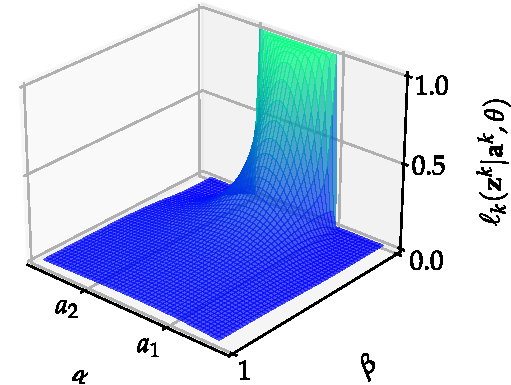
\includegraphics[width=4.6cm]{figures/PREM/likelihood_degen.pdf}\qquad
%     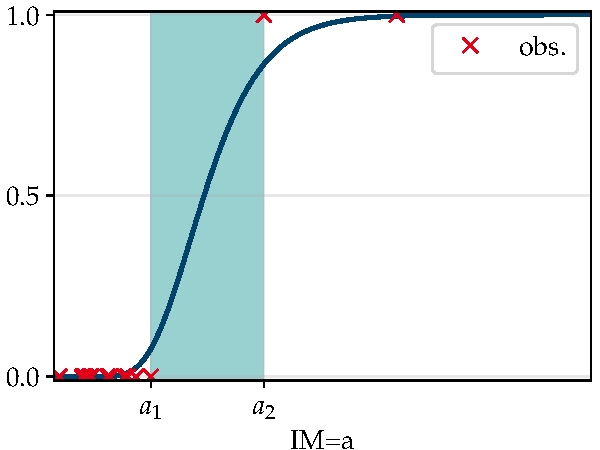
\includegraphics[width=4.44cm]{figures/PREM/degeneracy.pdf}
%     \caption{{Example of a type 3 data sample $(\mbf z^k,\mbf a^k)$ which gives a degenerate likelihood. Graphs of (left) the likelihood given the degenerate data sample as a function of the tuple $(\alpha,\beta)$ and (right) the fragility curve (blue curve) according to which the points (red crosses) are sampled : each red cross is a tuple $(z,a)$, where its X-axis equals $a$ and its Y-axis equals $z$.}
%     In both figures, $a_1$ is the maximal observed IM value among ``non-failures'', and $a_2$ is minimal one among ``failures''.
%     The interval $(a_1,a_2)$ (in cyan in the right figure) separates the failures and the non-failure observed.
%     }
%     \label{fig:constr-frags:degenerate-frag}
% \end{figure}



When the likelihood is degenerate, the vector $\mbf N$ is null and the likelihood does not shrink at $\beta\to0$.
As a consequence, the posterior will be proper only if the prior is proper w.r.t. $\beta$.
Moreover, in case of degeneracy of type 1 or 2, the likelihood does not shrink at either $\alpha\to\infty$ or $\alpha\to0$. In such a scenario, it becomes also essential to consider a prior that is proper  w.r.t. $\alpha$.

%Type 3
% In practice, cases of degeneracy of type 1 and type 2
% are more likely to appear if the equipment's failure criterion is  
% can appear if the structure failure criterion is 
% capture less attention. 
% Indeed, it makes sense that when we work with binary data, an observation set containing only failure outcomes, or containing only non-failure outcomes does not allow estimating appropriately a fragility curve.
In practice, cases of degeneracy of type 3 are the most critical ones since they are more likely to appear, especially when (i) the data are scarce, and (ii) the IM is more correlated with the system's response (see   \cref{app:chap:uncecomp}).


\section{Constrained reference prior for probit-lognormal fragility curves}\label{sec:constr-frags:constrained}


\subsection{Constrained reference prior framework}\label{sec:constr-frags:subsec-constr-frame}



To construct the prior, we take as a support the reference prior theory, whose principle is to maximize w.r.t. the prior the mutual information $\sI^k$. The mutual information is expected to measure the amount of information brought by the data over the \emph{a priori} information in the workflow. This methodology ensures the prior can be qualified as objective. We recall that this theory is completely reviewed in   \cref{chap:intro-ref}.
The mutual information can be written as a function of the prior $\varPi$:
\begin{equation}\label{eq:constr-frag:MI}
    \sI^k(\varPi) = \int_{\Theta}\int_{\cA^k}\sum_{\mbf z^k\in\{0,1\}^k}f\left(\frac{\int_\Theta\ell_k(\mbf z^k|\mbf a^k,\theta')d\varPi(\theta')  }{\ell_k(\mbf z^k|\mbf a^k,\theta)}\right)\ell_k(\mbf z^k|\mbf a^k,\theta)dH^{\otimes k}(\mbf a^k)d\varPi(\theta)  ,    
\end{equation}
where $f=-\log$ in the original theory, yet in this study we consider the mutual information written with $f=f_\delta:x\mapsto\frac{x^\delta-1}{\delta(\delta-1)}$, $\delta\in(0,1)$.
This corresponds to the generalized mutual information 
based on $\delta$-divergence, introduced in   \cref{chap:ref-generalized}. 

To be precise, the mutual information expression written in \cref{eq:constr-frag:MI} is not directly maximized w.r.t. $\varPi$, it is maximized asymptotically as $k\rightarrow\infty$ w.r.t. $\varPi$. We refer to   \cref{chap:intro-ref} or   \cref{chap:ref-generalized} for a more detailed definition of the reference prior. This asymptotic maximization is noted in this chapter as follows:
\begin{equation}\label{eq:constr-frag:optimnoconstr}
    \varPi^\ast\in\argmax_{\pi\in\cP;\,k\rightarrow\infty}\sI^k(\varPi),
\end{equation}
where $\cP$ is the set of all possible priors, namely the set of continuous $\sigma$-finite measures on $\Theta$.

It has been proven (see \cref{chap:intro-ref,chap:ref-generalized}) that the optimization problem~\eqref{eq:constr-frag:optimnoconstr} admits the Jeffreys prior as a solution. That prior is defined from its density $J$, expressed up to a constant as:
    \begin{equation}
        J(\theta)\propto\sqrt{|\det\cI(\theta)|}\quad\text{with}\quad \cI(\theta) = -\sum_{z\in\{0,1\}}\int_{\cA}\nabla_\theta^2\log\ell(z|a,\theta) \ell(z|a,\theta)dH(a).
    \end{equation}

As expressed in the introduction, we aim at applying the work done in   \cref{chap:constrained-prior}, in which it is suggested to add a constraint in the optimization problem~\eqref{eq:constr-frag:optimnoconstr}:
\begin{equation}\label{eq:constr-frag:optimconstr}
    \varPi^\ast\in\argmax_{\varPi\in\cP;\,k\rightarrow\infty}\sI^k(\varPi),\quad\text{subject to\ }\cC(\varPi)<\infty,
\end{equation}
where $\cC(\varPi)= \int a_c(\theta)d\varPi(\theta)$ for some function $a_c(\cdot)$.
That function is sought to regularize the Jeffreys prior decay rates. If it verifies
    \begin{equation}\label{eq:constr-frag:inta}
        \int_\Theta J(\theta)a_c(\theta)^{1+1/\delta}d\theta <\infty, \quad\text{and} \quad \int_\Theta J(\theta)a_c(\theta)^{1/\delta}<\infty 
    \end{equation}
then the prior whose density is proportional to $\theta\mapsto J(\theta)\cdot a_c^{1/\delta}(\theta)$ is the solution of problem~\eqref{eq:constr-frag:optimconstr}, and is a proper prior.


\subsection{Application to the probit-lognormal reference prior}\label{sec:constr-frags:subsec-constr-in-probit}


In   \cref{chap:prem}, the Jeffreys prior decay rates have been comprehensively studied.
We recall that
% \begin{equation}
    \begin{align}\label{eq:constr-frag:decaysJbeta}
        &\forall\alpha>0,\, J(\theta) \aseq{\beta\rightarrow0}\frac{D'(\alpha)}{\beta}\quad\text{and}\quad J(\theta)\aseq{\beta\rightarrow\infty}\frac{E'}{\alpha\beta^3}, \\
        &\forall\beta>0,\,J(\theta) \aseq{\log\alpha\rightarrow\pm\infty}G''(\beta)\frac{|\log\alpha|}{\alpha}\exp\left(-\frac{(\log\alpha-\mu)^2}{2\beta^2+2\sigma^2}\right),\label{eq:constr-frag:decaysJalpha}
    \end{align}
% \end{equation}
where $D'(\alpha)>0$ depends only on $\alpha$, $E'>0$ is a constant, and $G''(\beta)>0$ depends only on $\beta$.

The Jeffreys prior has an improper tail at $\beta\to0$ which does not shrinks when it is multiplied by a degenerate likelihood.
% This asymptotic rate at $\beta\to0$ is actually 
While we do not exactly know the shape of the prior on the whole domain, we assume that we can associate it to (i) an improper marginal distribution w.r.t. $\beta$ whose density follows asymptotically the rates in \cref{eq:constr-frag:decaysJbeta}, and (ii) a proper distribution of $\alpha$ conditionally to $\beta$.



It is thus possible to construct a constraint that will adjust the decay rate at $\beta\to0$ of the Jeffreys prior in order to make it integrable.
We chose $a_c(\theta)=\theta^\kappa$, that satisfies \cref{eq:constr-frag:inta} for $\kappa\in(0,\frac{2\delta}{1+\delta})$. 
The solution of the optimization problem~\eqref{eq:constr-frag:optimconstr} is then the prior whose density $\pi^\ast$ verifies $\pi^\ast(\theta)\propto J(\theta)\beta^{\kappa/\delta}$. In this work, we denote by $\varPi^\ast_\gamma$ this prior and by $\pi^\ast_\gamma$ its density, where $\gamma:=\kappa/\delta\in(0,\frac{2}{1+\delta})\subset(0,2)$:
    \begin{equation}
        \pi^\ast_\gamma(\theta) \propto J(\theta)\beta^\gamma.
    \end{equation}


%A little regularization of that decay rates allows to make it integrable.







%In our problem 


% \subsection{Theoretical expression of the prior}


\subsection{Practical derivation with integral interpolations}\label{sec:constr-frags:subsec-practical-interpol}


%In this section, we briefly recall the derivation process of the Jeffreys prior and 
The prior $\varPi_\gamma^\ast$ can be implemented by approximating numerically its density $\pi^\ast_\gamma$, using the theoretical expression of the Jeffreys prior.
We recall that, in   \cref{chap:prem}, we proved that %Jeffreys' density can be expressed as 
the Fisher information matrix can be expressed as 
\begin{equation}
    %\label{eq:infmat}
        \cI(\theta)=\begin{pmatrix}
        \frac{1}{\alpha^2\beta^2}(A_{01} + A_{02}) & \frac{1}{\alpha\beta^3}(A_{11}+A_{12}) \\
        \frac{1}{\alpha\beta^3}(A_{11}+A_{12}) & \frac{1}{\beta^4}(A_{21}+A_{22})
    \end{pmatrix},
    \end{equation}
by defining 
$A_{01}$, $A_{02}$, $A_{11}$, $A_{12}$, $A_{21}$, $A_{22}$ as
    \begin{equation} %\label{eq:Aij}
    \begin{aligned}
        %A_{11} &= \int_\cA\Phi'(\gamma)d\PP_A(a) & A_{12} &= \int_\cA\log\frac{a}{\alpha}\Phi'(\gamma)d\PP_A(a) \\
        A_{0u} &= \int_\cA\frac{\Phi'(\beta^{-1}\log\frac{a}{\alpha})^2}{\Phi((-1)^{u+1}\beta^{-1}\log\frac{a}{\alpha})}h(a)da,\\
        %& A_{02} &= \int_{\cA}\frac{\Phi'(\beta^{-1}\log\frac{a}{\alpha})^2}{\Phi(-\beta^{-1}\log\frac{a}{\alpha})}p(a)da,\\
        A_{1u} &= \int_\cA\log\frac{a}{\alpha}\frac{\Phi'(\beta^{-1}\log\frac{a}{\alpha})^2}{\Phi((-1)^{u+1}\beta^{-1}\log\frac{a}{\alpha})}h(a)da,\\
        %& A_{12} &= \int_{\cA}\log\frac{a}{\alpha}\frac{\Phi'(\beta^{-1}\log\frac{a}{\alpha})^2}{\Phi(-\beta^{-1}\log\frac{a}{\alpha})}p(a)da,\\
        A_{2u} &= \int_\cA\log^2\frac{a}{\alpha}\frac{\Phi'(\beta^{-1}\log\frac{a}{\alpha})^2}{\Phi((-1)^{u+1}\beta^{-1}\log\frac{a}{\alpha})}h(a)da,
        %& A_{22} &= \int_{\cA}\log^2\frac{a}{\alpha}\frac{\Phi'(\beta^{-1}\log\frac{a}{\alpha})^2}{\Phi(-\beta^{-1}\log\frac{a}{\alpha})}p(a)da,\\
    \end{aligned}
    \end{equation}
%reminding $\gamma=\beta^{-1}\log\frac{a}{\alpha}$.
for $u\in\{1,2\}$, and where $h$ denotes the p.d.f. of the IM.
%It is then 

Using the above, it is possible to approximate $J(\theta)$ by conducting Simpson's interpolations of the involved integrals in the Fisher information matrix. The interpolations are performed from a large dataset of IM values. We refer to   \cref{chap:frags-intro} where the seismic signal generator used in this work to provide
a large dataset of seismic signals is presented. The empirical distribution of the PGA of the seismic signals in that dataset is recalled in \cref{fig:constr-frags:PGA}. %That generator has been used to construct a dataset of $10^5$ seismic signals for which different IMs have been derived.
The interpolations are done a regular grid of $\cA=[a_{\min},a_{\max}]$, where $a_{\min}$ (resp. $a_{\max}$) is the minimal (reps. the maximal) value of the IM in the dataset.
The density $h$ is approximated by Gaussian kernel density estimation. 

Due to the computational cost of the numerical interpolations involved when approximating the Jeffreys prior, we conducted the same methodology as in   \cref{chap:prem}. This methodology consists in evaluating it on an experimental design based on a fine-mesh grid $\Theta$. These evaluations allow building an interpolated approximation of the Jeffreys prior density matching the design.
The density $\pi^\ast_\gamma$ is then obtained by multiplying the interpolated approximated Jeffreys by $\beta^\gamma$.

\begin{figure}[h]
    \centering
    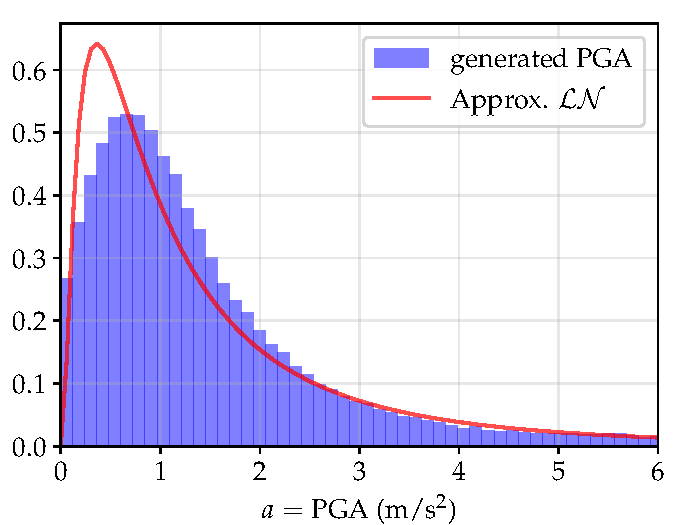
\includegraphics[width=5.2cm]{figures/constr-frags/pgadistrib.pdf}
    \label{fig:constr-frags:PGA}
    \caption{%
    Comparison of the histograms of the PGA values of generated signals (blue) with a lognormal
    density (red) that has same median (i.e. $0$) and same log deviation (i.e. $1$).}
    %approximations (red) for both IMs (PSA in the left figure, PGA in the right figure).}
\end{figure}





\section{Variational approximation of the constrained reference prior}\label{sec:constr-frags:varp}


\subsection{Definition of the VA-RP}\label{sec:constr-frags:subsec:varpdef}

The second approximation of the constrained reference prior that we conduct results form a variational inference methodology.
We recall that
variational inference encompasses a range of techniques designed to approximate probability distributions by solving an optimization problem (such as maximizing the evidence lower bound, as in \cite{kingma_auto-encoding_2014}). 
%For more information about variational inference, we refer to   \cref{chap:varp}.
Since our goal is to find
%Given that our objective involves finding 
the prior that maximizes the mutual information defined in \cref{eq:constr-frag:MI}, variational inference naturally lends itself to the approximation of reference priors.  

The approach that we conduct is based on the variational approximation of the reference prior (VA-RP) proposed in   \cref{chap:varp}.
It consists in limiting the family of priors to a parametric class $\{\varPi_\lambda,\,\lambda\in\Lambda\}$, with $\Lambda\subset\mathbb{R}^L$, thereby reducing the problem to a finite-dimensional setting. Consequently, the optimization tasks in equations \cref{eq:constr-frag:optimnoconstr,eq:constr-frag:optimconstr} %(  {eq:RPdef}) and (  {eq:def_const_RP}) 
translate into maximizing $\sI^k(\varPi_\lambda)$ over $\lambda\in\Lambda$. We define the priors $\varPi_\lambda$ implicitly through the transformation:
\begin{equation}
    \theta \sim \varPi_{\lambda} \iff \theta = g(\lambda,\varepsilon), \quad \text{where} \quad \varepsilon \sim \PP_{\varepsilon}.
\end{equation}
Here, $g$ is a parameterized measurable function ---typically a neural network--- where $\lambda$ represents its weights and biases, it has to be differentiable with respect to $\lambda$. The variable $\varepsilon$ serves as a latent variable, drawn from a simple, easy-to-sample distribution $\PP_\eps$. In practice, we choose a centered multivariate Gaussian $\mathcal{N}(0,I_{p\times p})$.  














\subsection{Optimization under constraints}\label{sec:constr-frags:subsec:optim}


The VA-RP is sought to approximate the solution of the optimization problems~\eqref{eq:constr-frag:optimnoconstr} or~\eqref{eq:constr-frag:optimconstr}.

To do so, the problem is considered for a fixed value of $k$. 
Also, instead of maximizing the mutual information, the method is maximizes the following objective function, which is a lower bound of the mutual information:
    \begin{equation}
        \lambda^\ast\in\argmax_{\lambda\in\Lambda} \cB^k(\varPi_\lambda),\quad \cB^k= \EE_{\theta\sim\varPi_\lambda}\sum_{\mbf z^k\in\{0,1\}^k}\int_{\cA^k}f_\delta\left(\frac{\ell_k(\mbf z^k|\mbf a^k,\hat\theta^{\text{MLE}})}{\ell_k(\mbf z^k|\mbf a^k,\theta)}\right) \ell_k(\mbf z^k|\mbf a^k,\theta)h(a)da,
    \end{equation}
where $\hat\theta^{\text{MLE}}$ refers to the maximum likelihood estimator: $\ell_k(\mbf z^k|\mbf a^k,\hat\theta^{\text{MLE}}) = \max_{\theta\in\Theta}\ell_k(\mbf z^k|\mbf a^k,\theta) $.


The optimization is conducted by stochastic gradient ascent, provided that the gradient of the objective function $\cB^k$ w.r.t. $\lambda$ is given by
    \begin{equation}
        \EE_{\eps\sim\PP_\eps}\left[\sum_{j=1}^{2}\partial_{\theta_j}\tilde\cB^k(g(\lambda,\eps))\nabla_\lambda g_j(\lambda,\eps)
        \right],
    \end{equation}
where the gradients of the neural network $\nabla_\lambda g(\lambda,\eps)$ are computed in the algorithm via automatic differentiation, and the terms $\partial_{\theta_j}\tilde\cB^k(g(\lambda,\eps))$  depend on the likelihood of % explicitly derived for 
the probit-lognormal model:
    \begin{equation}
        \partial_{\theta_j}\tilde\cB^k(\theta) = \sum_{\mbf z^k\in\{0,1\}^k}\int_{\cA^k} \partial_{\theta_j}\log\ell_k(\mbf z^k|\mbf a^k,\theta) F_\delta\left(\frac{\ell_k(\mbf z^k|\mbf a^k,\hat\theta^{\text{MLE}})}{\ell_k(\mbf z^k|\mbf a^k,\theta)}\right)\ell_k(\mbf z^k|\mbf a^k,\theta)h(a)da,
    \end{equation}
where $F_\delta(x) = f_\delta(x)-xf_\delta'(x)$.
The derivatives of the log-likelihood here equal the following:
    \begin{equation}
        \begin{aligned}
            &\partial_\alpha\log\ell_k(\mbf z^k|\mbf a^k,\theta) =  -\frac{1}{\alpha\beta}z\frac{\Phi'(\beta^{-1}\log\frac{a}{\alpha})}{\Phi(\beta^{-1}\log\frac{a}{\alpha})} + \frac{1}{\alpha\beta}(1-z)\frac{\Phi'(\beta^{-1}\log\frac{a}{\alpha})}{1-\Phi(\beta^{-1}\log\frac{a}{\alpha})} , \\
            &\partial_\beta\log\ell_k(\mbf z^k|\mbf a^k,\theta) = -\frac{\log\frac{a}{\alpha}}{\beta^2}z\frac{\Phi'(\beta^{-1}\log\frac{a}{\alpha})}{\Phi(\beta^{-1}\log\frac{a}{\alpha})}+ \frac{\log\frac{a}{\alpha}}{\beta^2}(1-z)\frac{\Phi'(\beta^{-1}\log\frac{a}{\alpha})}{1-\Phi(\beta^{-1}\log\frac{a}{\alpha})} .
        \end{aligned}
    \end{equation}



%The gradient ascent algorithm can be ad

Still following the method of   \cref{chap:varp},
the gradient ascent algorithm is adapted to approximate explicitly the solution of the optimization problem~\eqref{eq:constr-frag:optimconstr}.
This adaptation consists in actually solving
    \begin{equation}
        \lambda^\ast\in\argmax_{\lambda\in\Lambda}\cB^k(\varPi_\lambda)\quad\text{subject to\ } \cC(\varPi_\lambda)=0,
    \end{equation}
where $\cC(\varPi_\lambda)=\int_\Theta a(\theta)d\varPi_\lambda(\theta) - c/\cK$, with
    \begin{equation}
        \cK=\int_\Theta J(\theta)a(\theta)^{1/\delta}d\theta \quad\text{and}\quad
        c = \int_\Theta J(\theta)a(\theta)^{1+1/\delta}d\theta.
    \end{equation}
The above constants are derived using the numerical approximation of the Jeffreys prior density proposed in \cref{sec:constr-frags:subsec-practical-interpol}.
For more details on the conduction of the optimization process, we refer to   \cref{chap:varp}.



\subsection{Neural network architecture}\label{sec:constr-frags:architecture}


A single layer neural network is implemented for this problem. It takes the following form
\begin{equation}\label{eq:neuralnet-architecture}
    \eps \mapsto \begin{pmatrix}
        \mbf t_1(\eps)\\ \mbf t_2(\eps) 
    \end{pmatrix} \mapsto
          %
    \begin{pmatrix}
        \tilde\eps_1 = \mbf w_1^\top\mbf t_1(\eps) + b_1 \\
        \tilde\eps_2 = \mbf w_2^\top\mbf t_2(\eps)+b_2 
    \end{pmatrix} \mapsto
    \begin{pmatrix}
        \alpha = u_1(\tilde\eps_1)\\
        \beta = u_2(\tilde\eps_2)
    \end{pmatrix}.
\end{equation}
The coordinates of the vectors $\mbf w_1,\mbf w_2\in\RR^p$ and $\mbf b=(b_1,b_2)\in\RR^2$ constitute the weights of the neural network, they are initialized independently and randomly w.r.t. a Gaussian distribution. $\mbf t_1$, $\mbf t_2$, $u_1$, $u_2$ are activation functions.
They are specifically chosen in order to ensure the VA-RP's decay rates match with the ones of the target prior: $u_1=u_2=\exp$ and for $\mbf x\in\RR^p$, $\mbf t_1(\mbf x)=(t_1(x_i))_i$ and $\mbf t_2(\mbf x)=(t_2(x_i))_i$ with
\begin{equation}
    t_1(x) = x;\quad t_2(x) = \log(1-\Phi(x)),
\end{equation}
%where $\Phi$ designates the c.d.f. of a standard Gaussian.
In \cref{sec:constr-frags:app}, we prove that under those settings the VA-RP yields marginal distributions $ p_\alpha$, $p_\beta$ w.r.t. $\alpha$, $\beta$, that take the following form:
    \begin{equation}
        \begin{aligned}
        p_\alpha(\alpha) &= \frac{1}{\alpha\sqrt{2\pi}\|\mbf w_1 \|_2}\exp\left(-\frac{(\log\alpha - b_1)^2}{2\|\mbf w_1\|^2_2}\right) \\
        p_\beta(\beta) &= \sum_{i,\, w_{2i}>0}{K_i}\beta^{-\frac{1}{w_{2i}}-1}\indic_{\beta>e^{b_2}} + \sum_{i,\, w_{2i}<0}K_i\beta^{-\frac{1}{w_{2i}}-1}\indic_{\beta<e^{b_2}},
    \end{aligned}
    \label{eq:marginaldist}
    \end{equation}
where $(w_{2i})_{i=1}^p$ denote the coordinates of $\mbf w_2$, and the $K_i$ are constants that depend on $\mbf w_2$ and $b_2$. 
The marginal distribution $p_\alpha$ is a log-normal distribution, which is similar, up to the $\log \alpha$ term, to the Jeffreys prior decay rates w.r.t. $\alpha$ (\cref{eq:constr-frag:decaysJalpha}).  Concerning $p_\beta$, calling $w_{2j}^{-1}=\min\{w_{2i}^{-1},\,w_{2i}>0\}$ and $w_{2l}^{-1}=\max\{w_{2i}^{-1},\,w_{2i}<0\}$, 
it admits the following decay rates:
\begin{equation}
    p_\beta(\beta)\equi{\beta\rightarrow0} K_j\beta^{-\frac{1}{w_{2l}}-1};\quad p_\beta(\beta)\equi{\beta\rightarrow\infty} K_l\beta^{-\frac{1}{w_{2j}}-1}.
    \label{eq:palphabeta}
\end{equation}
They are consistent with the ones of the Jeffreys prior. % (resp. the $\gamma$-constrained Jeffreys prior), if $\frac{1}{w_{2j}}$









%we approximate the solution of the constrained optimization problem (\cref{eq:constr-frag:optimconstr}) by solving the optimization problem





% \subsection{Posterior sampling}

%This implicit construction provides considerable flexibility in defining prior distributions. However, except in simpler cases, the density function of $\pi_\lambda$ remains unknown and cannot be evaluated directly. Instead, we obtain samples $\theta\sim\pi_\lambda$.  








\section{Comparison between the VA-RP and the interpolated reference prior}\label{sec:constr-frags:coparisonpriors}


% \subsection{}

In this section, we compare the approximation of the target prior using the VA-RP approach with the approximation by numerical interpolation of the theoretical expression of the Jeffreys prior density (denoted AJ).
We consider that the AJ is a more accurate approximation of the target than the VA-RP. For this reason, this section mostly serves the assessment of the VA-RP methodology in the context of the probit-lognormal model.

We implemented the probit-lognormal modeling assuming that the p.d.f. h of the IM is defined by
%We have implemented the probit-lognormal modeling by setting the p.d.f. $h$ of the IM as
    \begin{equation}\label{eq:constr-frags:ha}
        h(a) = \frac{1}{\sqrt{2\pi}\sigma_a^2 a}\exp\left(-\frac{(\log a-\mu_a)^2}{2\sigma_a^2}\right)
    \end{equation}
with
$\mu_a=0$ and $\sigma_a=1$. These parameters, which define the distribution of $a$, are the only elements that have a theoretical impact on the reference prior.
Their value are derived to fit the empirical distribution of the PGA values of the seismic signals that we consider. That empirical distribution is compared with the p.d.f. of \cref{eq:constr-frags:ha} in \cref{fig:constr-frags:PGA}.
%Their values are derived from the case study which is considered in \cref{sec:constr-frags:appasg}.
%  Section~{sec:case-study}.





\paragraph{Training of the unconstrained VA-RP}
First, we present the training process of the unconstrained VA-RP. It is expected to approach the unconstrained reference prior, i.e. the Jeffreys prior. 
%The latter being improper, we expect the training to 
% irregularities 
% The 
As for the different parameters 
for the training, we take $k=50$ and $p=50$. The training consists in the maximization of $\cB^k$ with $\delta=0.5$. 
The optimization has been done through a number of $9000$ epochs, with a learning rate of $0.005$.


\Cref{fig:unconstr_weights} shows the evolutions of the weights of the neural network that define the marginal distributions of $p_\alpha$ and $p_\beta$ (see \cref{eq:marginaldist}), as a function of the number of epochs. Thus, the bias $b_1$ is constant and equal to $0$, which is consistent with the asymptotic distribution of $\alpha$. $1/w_{2l}$ and $1/w_{2j}$ both tend to $0$. As a result, the marginal distribution of $\beta$ tends to $1/\beta$. This is an improper distribution which does not exactly match the expected improper Jeffreys prior (see \cref{eq:constr-frag:decaysJbeta}): it has a heavier tail as $\beta\to\infty$ than the original Jeffreys. 
However, we will see at the end of this section that the information contained in the distribution is not concentrated in its tails. In reality, low values of $\beta$ have huge weights
%However, we will see in the end of this section that the distribution is not limited to its tails, and that this prior actually ascribes huge weights to small values of $\beta$ 
(see the paragraph ``Posterior evaluation''). Finally, $\|\mbf w_1\|_2$ tends to $+\infty$. This means that the variance of  $\log\alpha$ tends to $+\infty$ as it is expected (see \cref{sec:constr-frags:app}), even though this does not lead to the target distribution. This last result is nevertheless not surprising. It is the consequence of the chosen architecture of the VA-RP: $p_\alpha$ is a lognormal distribution (\cref{eq:palphabeta}), which is not exactly the case for the Jeffreys prior (\cref{eq:constr-frag:decaysJalpha}). What fundamentally distinguishes these two distributions is that (i) in the first case, that of Jeffreys, the variance of $\log\alpha$ is finite conditionally to $\beta$, and is infinite otherwise because of the heavy tail of the distribution w.r.t. $\beta$ %is infinite because of the heavy tail of the distribution
while (ii) in the second case, the variance becomes infinite to correspond, via the training process, to the target variance of the Jeffreys prior. In doing so, the marginal distribution of $\alpha$ tends towards the improper distribution $1/\alpha$. Although this result is open to criticism, it appears to be an ``acceptable'' compromise insofar as the model's likelihood tends to substantially attenuate the prior's tails with respect to $\alpha$, thereby limiting the influence of the prior's decay rates on the posterior. An alternative approach could involve modifying the neural network architecture to better capture the correlation between $\alpha$ and $\beta$. However, such adjustments would inevitably increase the computational complexity of the training process.


\begin{figure}[h]
    \centering
    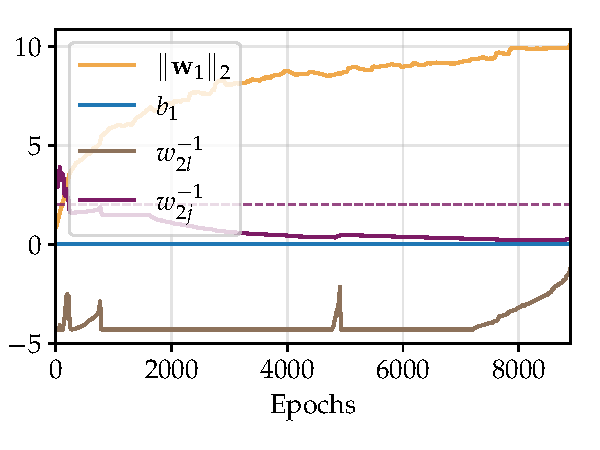
\includegraphics[width=5.2cm]{figures/constr-frags/weights_unconstr.pdf}
    \caption{
        Weights of interest of the neural network during the unconstrained optimization. %The yellow and blue curves represent respectively $\|\mbf w_1 \|_2$ and $|b_1|$, where $\|\mbf w_1 \|_2^2$ is the variance of the log of the first component, and $b_1$ its mean. 
    The brown and violet curves represent respectively $1/w_{2l}$ and $1/w_{2j}$ that are defined in \cref{sec:constr-frags:architecture}. In violet dashed line is plotted the target value of $1/w_{2j}$. % plotted their target value.
    %Parameters of interest of the neural network during the unconstrained optimization. The yellow and blue curves represent respectively $\|\mbf w_1 \|_2$ and $|b_1|$, where $\|\mbf w_1 \|_2^2$ is the variance of the log of the first component, and $b_1$ its mean. The brown and violet curves represent respectively $1/w_{2l}$ and $1/w_{2j}$ which appear in the decay rates of the second component.
    }
    \label{fig:unconstr_weights}
\end{figure}



\paragraph{Training of the constrained VA-RP}
As for the constrained case, we remind that we introduce a constraint of the form $\cC(\varPi_\lambda)=0$ with  $\cC(\varPi_\lambda) = \int_\Theta \beta^\kappa d\varPi_\lambda - \cK/c$.
We fix $\kappa=0.15$, so that $\gamma=\kappa/\delta=0.3$.
In this case the VA-RP is expected to approximate the constrained reference prior, i.e. the prior whose density  $\pi^\ast$ is proportional to $\theta\mapsto J(\theta)\beta^\gamma$.
Its asymptotic rates are identical to those of the Jeffreys prior for $\alpha$. If we fix $\alpha$, we have then:
\begin{equation} 
\begin{cases} \displaystyle
\pi^\ast(\theta) \propto \beta^{\gamma -1} \quad \text{as} \quad  \beta \longrightarrow 0 \\
\pi^\ast(\theta) \propto \beta^{\gamma - 3} \quad \text{as} \quad  \beta \longrightarrow +\infty.
\end{cases} 
\end{equation} 
In this case, the development done in \cref{sec:constr-frags:app} suggests that this prior verifies $\EE_{\theta\sim\pi^\ast}|\log\alpha|^2=\infty$.
The training process of the constrained VA-RP is done during $12000$ epochs with a learning rate of $0.001$. %We take $N=50$, $T=50$ and $p=50$. the parameter $\eta$ in the augmented Lagrangian is updated every $10$ epochs.



\Cref{fig:constr-frags:training-constr}.(a) suggests that the constraint seems reasonably verified during the whole optimization as the constraint gap is close to zero and appears to be decreasing. \Cref{fig:constr-frags:training-constr}(b) shows that the inverse weights $1/w_{2l}$ and $1/w_{2j}$ appear to steadily approach their theoretical values, respectively $-\gamma=-0.3$ and $2-\gamma = 1.7$. As in the unconstrained case, we observe that $\|\mbf w_1\|_2$ tends to $+\infty$. This is consistent with the theoretical results of \cref{sec:var_prior_alpha} which suggest, recall, that for all $\gamma\geq0$, $\EE[|\log\alpha|^2]=\infty$. So, we verify that adding constraints therefore allows, as expected, to ``control'' the distribution of $\beta$. Concerning $\alpha$, we find the same trend as in the unconstrained case, which is theoretically expected from the point of view of the variance of the marginal distribution.


\begin{figure}[h]
    \centering
    %\begin{tabular}{@{}c@{}}		
	%\subfloat[Constraint value gap. \label{fig:constr_gap}]
    {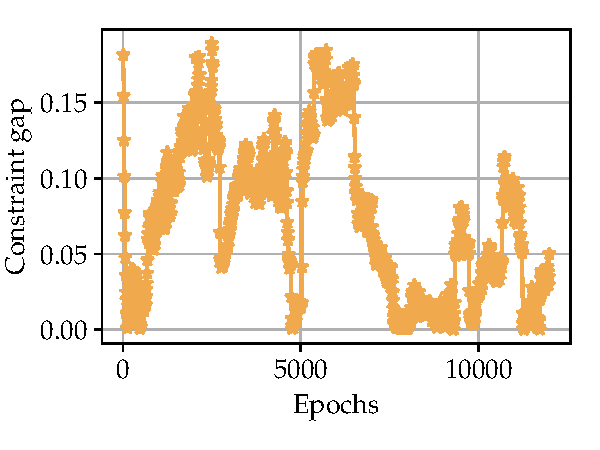
\includegraphics[width=5.2cm]{figures/constr-frags/constraint gap.pdf}}
    %\end{tabular}
    %\hspace{-0.2cm}    
    %\begin{tabular}{@{}c@{}}		
	%\subfloat[Weights of interest of the neural network. \label{fig:constr_weights} ]
    {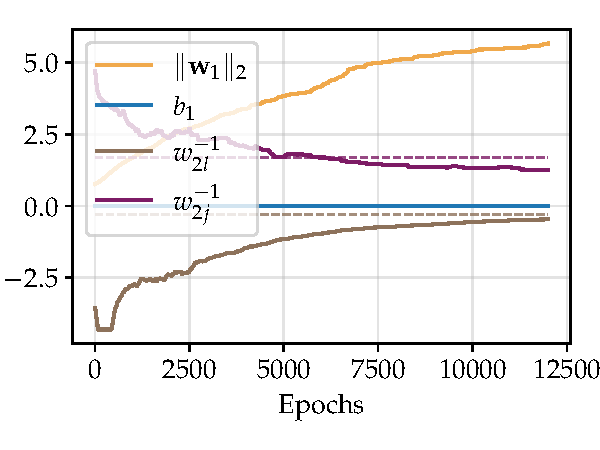
\includegraphics[width=5.2cm]{figures/constr-frags/weights_constr.pdf}}
    \makebox[5.2cm]{(a)}\makebox[5.2cm]{(b)}
    %\end{tabular}
  \caption{(a) Evolution of the constraint value gap during training. It corresponds to the difference between the target and current values for the constraint (in absolute value). (b) Weights of interest of the neural network during the constrained optimization. The yellow and blue curves represent respectively $\|\mbf w_1 \|_2$ and $b_1$, where $\|\mbf w_1 \|_2^2$ is the variance of the log of the first component, and $b_1$ its mean. The brown and violet curves represent respectively $1/w_{2l}$ and $1/w_{2j}$ that are defined in \cref{sec:constr-frags:architecture}. In same color dashed line are plotted their target value.\label{fig:constr-frags:training-constr}}
% \label{fig:constr_gap_weights}    
\end{figure}

%str_weights}
%\end{figure}

\paragraph{Posterior evaluation}
We evaluate the posterior that the VA-RPs derived in this section yield.
For this purpose, we take as dataset $k=50$ samples $(\mbf z^k,\mbf a^k)$, $\mbf z^k=(z_i)_{i=1}^k$, $\mbf a^k=(a_i)_{i=1}^k$, that are generated given a probit-lognormal model with $\theta_{\text{true}}$ close to $(3.37, 0.43)$. %The distribution of. % considered is still a log-normal with $\mu_a=0$ and $\sigma_a=1$.

\emph{A posteriori} samples are generated for both approaches by using an adaptive Metropolis-Hasting (M-H).
In the case of the AJ approach, the M-H is implemented to generate samples using the approximated posterior density.
In the case of the VA-RP, the M-H is implemented to generate samples using the posterior density $q(\cdot|\mbf z^k,\mbf a^k)$ density of $\eps$:
    \begin{equation}
        q(\eps|\mbf z^k,\mbf a^k) \propto q(\eps)\ell_k(\mbf z^k|\mbf a^k,g(\lambda,\eps)),
    \end{equation}
where $q(\cdot)$ denotes the p.d.f. of $\eps$.
\emph{A posteriori} samples of $\theta$ are obtained by applying the neural network $g(\lambda,\cdot)$ to the \emph{a posteriori} samples of $\eps$.
For both methods, a number of $5000$ samples of $\theta$ are generated this way.
In this example, 
we precise that the likelihood is not degenerate.
% For the sake of completeness, they are compared with samples generated considering an other prior: the actual reference prior derived by approximating numerically its theoretical expression, as depicted in \cite{van2024reference}. 
% The samples are generated by an other adaptive Metropolis-Hastings algorithm, which iteratively evaluates the prior. In the following, we refer to the latter as AJ.

%For the posterior, we take as dataset $50$ samples from the probit model with $\theta_{true}$ close to $(3.37, 0.43)$. The adaptive Metropolis-Hastings algorithm on $\varepsilon$ is applied for $10^5$ iterations, the last $5000$ a posteriori samples are kept. 


%We would like to avoid the situation where the data points are partitioned into two disjoint subsets when classified according to $a$ values. In that case, the posterior becomes improper because the likelihood is constant (\cite{van2024reference}), we say that the dataset is degenerate.


%we have not retained the samples for which the data are dissociated into two disjoint subsets when they are classified according to the values of $a$. In this case, indeed, the posterior distribution is improper because the likelihood is constant when $\beta$ tends to 0 \cite{van2024reference}. We then say that the dataset is degenerate \cite{AVB2025}. The probability of occurrence of such datasets is not negligible if the dataset has a small size. The following plots are obtained with non-degenerate datasets. 


\begin{figure}[h]
    \centering
    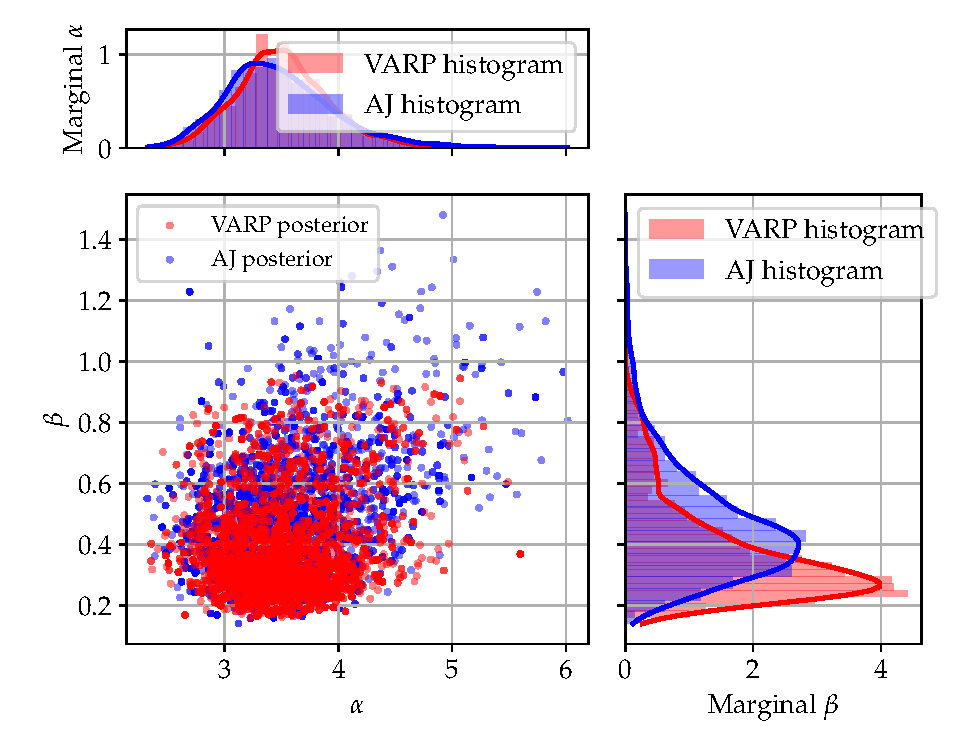
\includegraphics[height=7cm]{figures/constr-frags/hist_post_marg_unconstrained_new.pdf}%
    \caption{Scatter histogram of the unconstrained VA-RP posterior and the approximated Jeffreys (AJ)  posterior distributions obtained from $5000$ samples. Kernel density estimation is used on the marginal distributions in order to approximate their density functions with Gaussian kernels.}
    \label{fig:scatterhist_unconstr}
\end{figure}

\begin{figure}[h!]
    \centering
    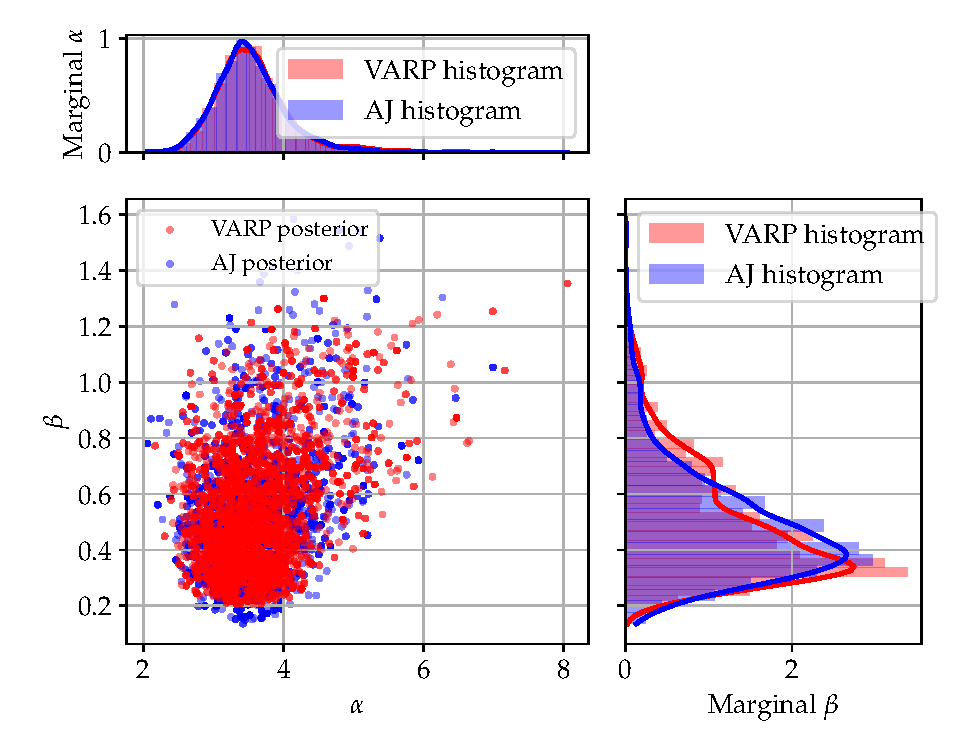
\includegraphics[height=7cm]{figures/constr-frags/hist_post_marg_constrained_new.pdf}
    \caption{Scatter histogram of the constrained VA-RP posterior and the approximated Jeffreys (AJ)  posterior distributions obtained from $5000$ samples. Kernel density estimation is used on the marginal distributions in order to approximate their density functions with Gaussian kernels.}
    \label{fig:scatterhist_constr}
\end{figure}



\Cref{fig:scatterhist_unconstr,fig:scatterhist_constr} show that the posterior distribution obtained from the VA-RP looks more like Jeffreys prior %more closely resembles to the Jeffreys prior 
in the constrained case than in the unconstrained one. 
More specifically, w.r.t. $\alpha$, the VA-RP is similar to the Jeffreys prior in both cases. That suggests that the limitation of our neural network architecture discussed earlier has little impact on the posterior distribution.
Regarding $\beta$,
in the unconstrained case, the VA-RP ascribes predominant weight to smaller values of $\beta$ compared to the Jeffreys prior, with a mode that is closer to $0$. In terms of fragility curve estimation that could represent an issue, as it may lead to estimates with thinner credibility intervals around a fragility curve. %that approximates an ---irrealistic--- unit-step function.









\section{Application of the method on the piping system case study}\label{sec:constr-frags:appasg}


In this section, we propose to apply the VA-RP that we have constructed and optimized above
% in what precedes 
to an industrial problem.
The industrial problem,  consists in the piping system that was introduced in   \cref{chap:frags-intro} (\cref{sec:intro-frags:casstudies}). 
This application serves as a proof of concept, we intend to show that the constrained VA-RP allows estimating efficiently and accurately seismic fragility curves in practice.

We recall that a validation dataset made of $8\cdot 10^4$ samples is available for this case study and permit constructing a reference fragility curves $P_f^{\text{ref}}$ following the non-paramteric method described in \cref{chap:frags-intro} (\cref{sec:intro-frags:models}).
In this study, we consider the PGA as IM.





% \subsection{Case study description as a reminder}\label{sec:constr-frags:subsec:asgdesc}


% The studied mechanical system consists in a piping system that comes from the secondary cooling circuit of a French pressurized water reactor.
% The piping was presented in details in   \cref{chap:frags-intro} (\cref{sec:intro-frags:piping}) and is illustrated in \cref{fig:constr-frag:asg}.
% The mock-up has submitted to artificial seismic signals on a shaking table that permits to validate a finite element model, which simulates the structure's response under seismic excitations.
% A total of $8\cdot 10^4$ nonlinear dynamical simulations have been carried out given seismic signals that were taken from the dataset of $10^5$ signals that we dispose. These results serve as a validation dataset. 
% The engineering demand parameter (EDP) for this structure corresponds to the out-of-plane rotation of its first elbow (see the details in   \cref{chap:frags-intro}), the results of the simulations are plotted in the plan (PGA,EDP) in \cref{fig:constr-frag:asg}-middle.
% In \cref{fig:constr-frag:asg}-right, reference fragility curves given different rotation threshold are derived for this structure. They are computed using the non-paramteric method proposed by \citet{trevlopoulos_parametric_2019} and detailed in   \cref{chap:frags-intro} (\cref{sec:intro-frags:subsec-nonparametric}).






% \begin{figure}[h]
%     \centering
%     \parbox[b][3.8cm][c]{4.5cm}{%
%     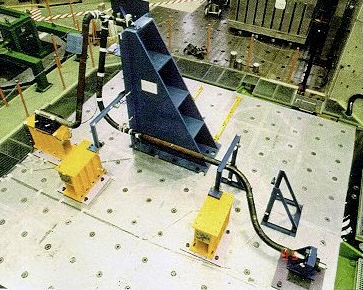
\includegraphics[height=3.2cm]{figures/intro-frags/ASG.jpg}\vspace*{1em}%
%     }
%     \includegraphics[height=3.8cm]{figures/intro-frags/asg/cloud_PGA_light.pdf}\ \ 
%     \includegraphics[height=3.8cm]{figures/intro-frags/asg/refs_PGA.pdf}
%     \caption{Illustration of the case study. Left: picture of the mock-up on the Azalee shaking table of CEA. Middle: results of $8\cdot10^4$ non-linear dynamical simulations. Right: reference non-parametric fragility curves (dashed lines) surrounded by their $95\%$-confidence intervals, compared with the probit-lognormal fragility curves derived by MLE from the validation dataset of size $10^5$. Different threshold $C$ are considered, each yields different proportions of failures in the validation dataset: resp. $95\%$ (red), $90\%$ (purple) and $85\%$ (blue).}
%     \label{fig:constr-frag:asg}
% \end{figure}



\subsection{Benchmarking metrics}\label{sec:constr-frags:subsec:benchmarking}


In this chapter, we evaluate our estimates by comparing them to the reference fragility curve $P^{\text{ref}}_f$ that is derived using a validation dataset. %As %explained in the previous subsection, the reference is computed using a non-paramteric method implemented from the available validation dataset of $8\cdot 10^4$ samples.
We recall that the reference was compared in \cref{chap:frags-intro} to a probit-lognormal curve $P^{\text{MLE}}_f$ whose parameters are estimated by maximum likelihood estimation using the same validation dataset.
%In \cref{fig:constr-frag:asg},
% different fragility curves, derived considering different excessive rotation threshold for defining the equipment's failure are elucidated. 
% In this study, the failure of the system was defined when the EDP exceeded $C=3.8^\circ$.
%in Figure~  {fig:refs}.
% The reference $P^{\text{ref}}_f$ is compared to a probit-lognormal curve $P^{\text{MLE}}_f$ whose parameters are estimated by maximum likelihood estimation using the same validation dataset.
%Each are compared with a probit-lognormal curve $P^{\text{MLE}}_f$, derived implementing a maximum likelihood estimate of the probit-lognormal fragility curve using the full batch of the $8\cdot 10^4$ results depicted in Figure~  {fig:cloud_data}. 
That comparison demonstrates the adequacy of such modeling of the fragility curve. However, it also emphasizes an existing bias that the model has compared with the non-parametric estimate. In the following, we refer to this difference between $P_f^{\text{MLE}}$ and $P_f^{\text{ref}}$ as the square model bias, denoted by $\cM\cB$:
\begin{equation}
    \cM\cB = \|P^{\text{ref}}_f - P^{\text{MLE}}_f  \|_{L^2}^2;
\end{equation}
where the norm $\|\cdot \|_{L^2}$ is defined by $\|P\|_{L^2}^2=\int_{a_{\min}}^{a_{\max}} P(a)^2da$ where the domain $[a_{\min},a_{\max}]
$ covers the available seismic signals. The norm is derived numerically from Simpson's interpolation. % on a regular sub-division of $(0,\infty)$.




Given an observed sample of size $k$: $(\mbf z^k,\mbf a^k)$, $\mbf z^k=(z_i)_{i=1}^k$, $\mbf a^k=(a_i)_{i=1}^k$, we denote by $P_f^{|\mbf z^k,\mbf a^k}:a\mapsto \Phi(\beta^{-1}\log (a/\alpha))$ the process whose distribution inherits from the posterior distribution  of $\theta$ conditionally to $(\mbf z^k,\mbf a^k)$. For any value of $a$, we note $q_{r}^{|\mbf z^k,\mbf a^k}(a)$ the $r$-quantile of $P^{|\mbf z^k,\mbf a^k}_f(a)$, and $m^{|\mbf z^k,\mbf a^k}(a)$ its median.
We propose to evaluate our estimates using the following metrics:
\begin{itemize}
    \item The square bias to the median $\cB^{|\mbf z^k,\mbf a^k}=\|m^{|\mbf z^k,\mbf a^k}-P^{\text{ref}}_f\|^2_{L^2}$.
    \item The square credibility width $\cW^{|\mbf z^k,\mbf a^k}=\|q_{1-r/2}^{|\mbf z^k,\mbf a^k} - q_{r/2}^{|\mbf z^k,\mbf a^k}\|^2_{L^2}$, with $r=0.05$.
    \item The upper quantile error $\cQ^{|\mbf z^k,\mbf a^k}=\|q_{1-r/2}^{\mbf z^k,\mbf a^k}-P_f^{\text{ref}} \|^2_{L^2}$.
\end{itemize}
%
% For comparison purpose, we suggest to derive the above metrics 
The quantiles and the medians are approximated using generated samples.









\subsection{Results}\label{sec:constr-frags:subsec:results}




%In this section, we compare the evaluation of our estimates that results from using the VA-RP with the evaluation of the ones that result from using an approximation via numerical derivation of the Jeffreys prior. In the following, we refer to the latter as AJ.
%Both are implemented with and without the incorporation of a constraint that is tailored to ensure they are proper. The considered constraint is detailed in Section~  {sec:varp-implementation}.


In \cref{fig:frag-ex-asg} we provide examples of \emph{a posteriori} fragility curves credibility intervals yielded by the two priors, with and without incorporating a constraint on the decay rates.
These examples arise from given samples of $k=80$ observations. They illustrate that the VA-RP is capable of providing fragility curve estimates that are equivalent of the ones provided by the AJ, which is an approximation of the exact expression of the reference prior.


\begin{figure}[h]
    \centering
    % \begin{tabular}{@{}c@{}}		
	% \subfloat[\label{fig:ex_ASG_unconstr50}]{
    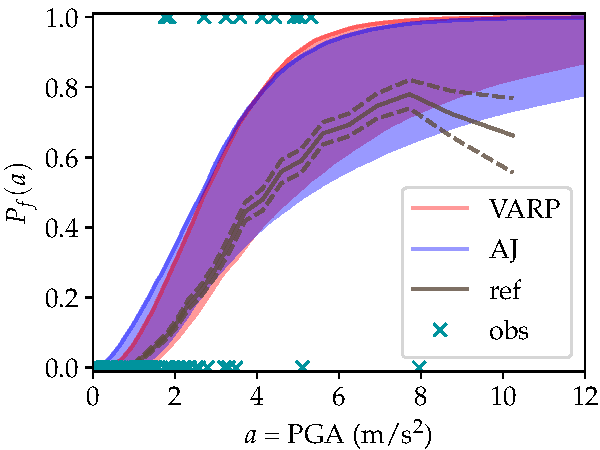
\includegraphics[width=5cm]{figures/constr-frags/ex_ASG_unconstr80.pdf}\ %}
    % \end{tabular}
    % \hspace{0.1cm}
    % \begin{tabular}{@{}c@{}}		
	%\subfloat[\label{fig:ex_ASG_constr50}]{
    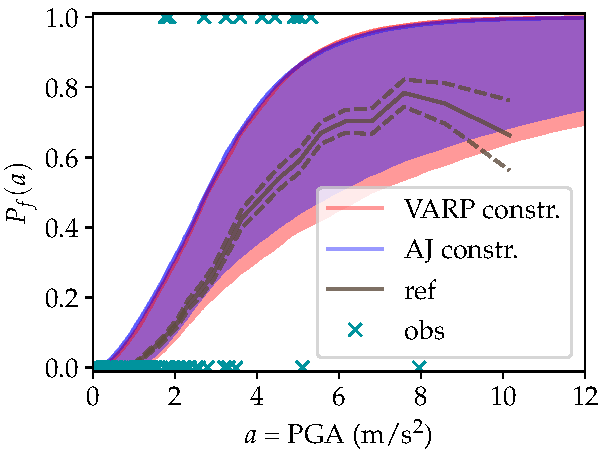
\includegraphics[width=5cm]{figures/constr-frags/ex_ASG_constr80.pdf}\\%
    \makebox[5cm]{(a)}\ \makebox[5cm]{(b)}
    % \end{tabular}
    \caption{Example of \emph{a posteriori} $95\%$ credibility intervals yielded by the posterior distribution resulting from a sample of $k=80$ data and from the VA-RP (in red) or the AJ (in blue)~: (a) unconstrained priors and (b) constrained priors.
    The reference curve $P^{\text{ref}}_f$ (solid line) is surrounded by its $95\%$ confidence interval (dashed line) in each figure. The cyan crosses represent the observed sample.}
    \label{fig:frag-ex-asg}   
\end{figure}



To deepen the comparison, 
we implemented the methods multiple times for values of $k$ varying in $[10,250]$. More precisely, for each $k\in\{10,20,\dots,250\}$, $10$ random data samples of size $k$ have been drawn. Each of these samples were then used to compute the metrics $\cB^{|\mbf z^k,\mbf a^k}$, $\cW^{|\mbf z^k,\mbf a^k}$ and $\cQ^{|\mbf z^k,\mbf a^k}$.

The average values of these metrics along with their $95\%$ confidence intervals are presented in \cref{fig:errors-unconstrained} (for the unconstrained case) and \cref{fig:errors-constrained} (for the constrained case) as functions of $k$.






\Cref{fig:errors-unconstrained,fig:errors-constrained} confirm previous results on a larger scale, namely that, with the current architecture, the constrained VA-RP outperforms the unconstrained VA-RP. Regarding bias, for example, it produces less erratic results. Compared to the AJ approximation, the VA-RP approximations exhibit slightly larger biases. The gap decreases as the number of data increases as expected, but only in the constrained case. Regarding the sizes of the credibility intervals (the values of $\cW^{|\mbf z^k,\mbf a^k}$), they are generally smaller in the unconstrained case. This result is consistent with the observation made in \cref{fig:scatterhist_unconstr} concerning the marginal distribution of $\beta$. This shows smaller values than with the AJ approximation of the Jeffreys prior.
It is important to emphasize that it is primarily the lower bounds of the credibility intervals that are ``penalized'' with the constrained VA-RP approximation. The upper bound remains consistent with that of the AJ, as reflected in the values of $\cQ^{|\mbf z^k,\mbf a^k}$. This result illustrates the relevance of using the constrained VA-RP approach for safety study. Indeed, in such a context, focusing on the upper quantile is consistent with a conservative approach.







\begin{figure}[h]
    \centering
    \makebox[0pt]{%
    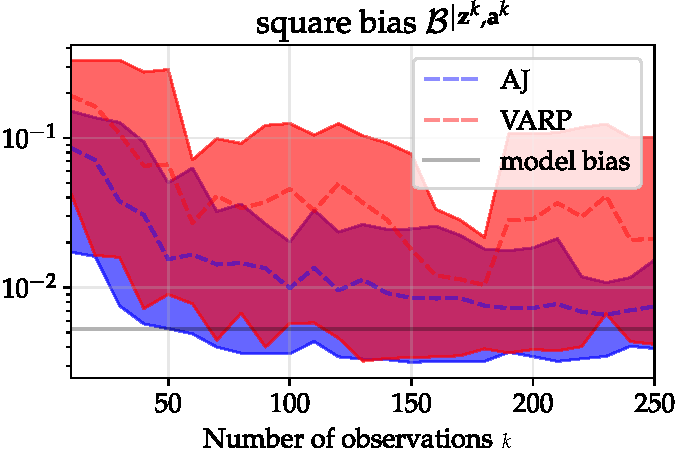
\includegraphics[width=5cm]{figures/constr-frags/errB_n.pdf}%
    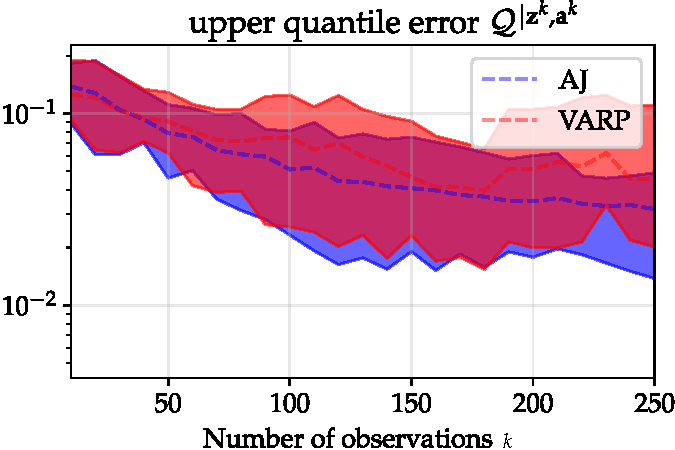
\includegraphics[width=5cm]{figures/constr-frags/errQ_n.pdf}%
    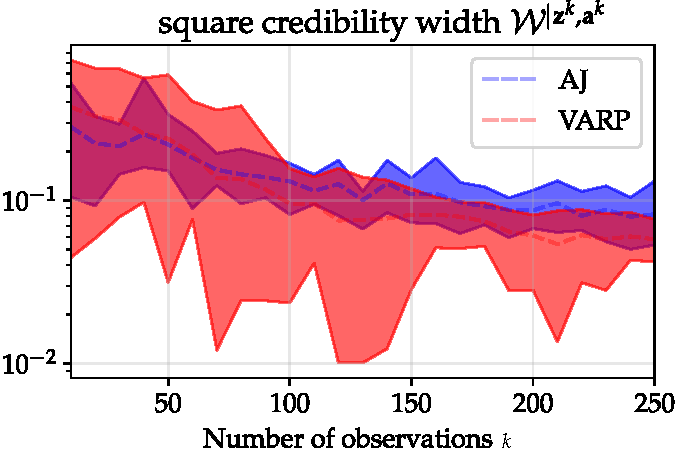
\includegraphics[width=5cm]{figures/constr-frags/errW_n.pdf}%
    }
    \caption{Average errors (dashed line) $\cB^{|\mbf z^k,\mbf a^k}$, $\cQ^{|\mbf z^k,\mbf a^k}$, $\cW^{|\mbf z^k,\mbf a^k}$ and their $95\%$ confidence intervals, derived from numerical replications of the unconstrained methods for each value of $k$ in $\{10,20,\cdots,250\}$. The values derived 
    using the VA-RP (red) are compared with the ones 
    using a numerical derivation to approximate the Jeffreys prior (blue). In the left figure, the square model bias $\cM\cB$ is plotted (solid line).}
    \label{fig:errors-unconstrained}
\end{figure}




\begin{figure}[h]
    \centering
    \makebox[0pt]{%
    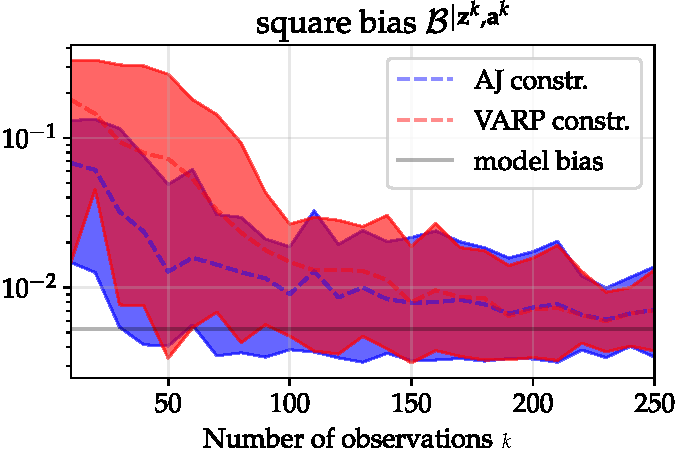
\includegraphics[width=5cm]{figures/constr-frags/errB_c.pdf}%
    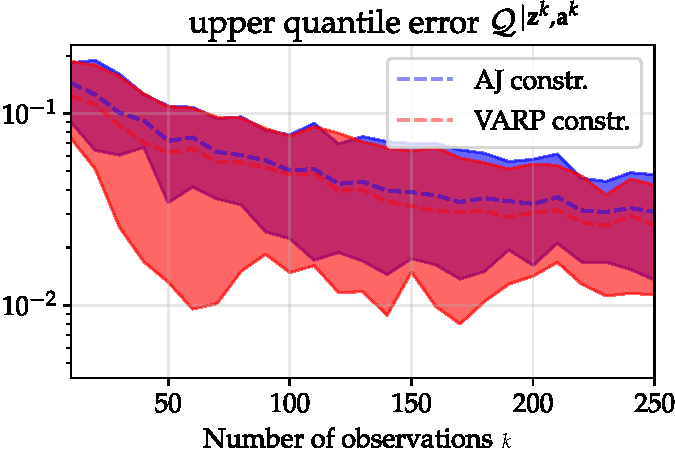
\includegraphics[width=5cm]{figures/constr-frags/errQ_c.pdf}%
    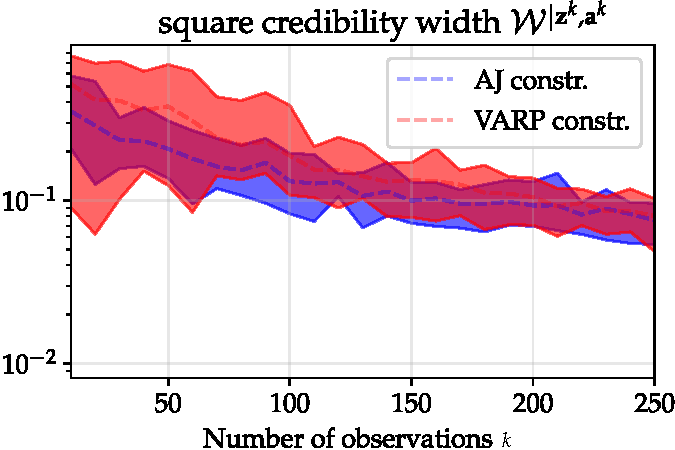
\includegraphics[width=5cm]{figures/constr-frags/errW_c.pdf}%
    }
    \caption{Same as \cref{fig:errors-unconstrained}, but when a constraint is incorporated in the priors.}
    \label{fig:errors-constrained}
\end{figure}









\section{Impacts of the neural network's architecture on the VA-RP}\label{sec:constr-frags:app}




\subsection{Decay rates of the VA-RP density}\label{app:decay-rates}

In this section we elucidate the form taken by the marginal distribution of the VA-RP w.r.t. $\beta$.
The VA-RP is assumed to be expressed as presented in \cref{sec:constr-frags:architecture} (\cref{eq:neuralnet-architecture}): the random variable $\beta$ is defined as
    \begin{equation}\label{eq:app-expr-beta}
        \beta = \exp\left[\sum_{i,\,w_{2i}\ne0}w_{2i}\log(1-\Phi(\eps_i)) + b_i\right],
    \end{equation}
where the $(\eps_i)_i$ are independent standard Gaussian variables.
%As the weights $(w_{2i})_i$ are initialized 
We recall that the weights $(w_{2i})_{i}$ are initialized randomly w.r.t. a Gaussian distribution. Therefore, they have almost surely 
% we reasonably suppose that they have 
distinct absolute values.
We rely on the two following lemmas.
\begin{lem}\label{lemma:expon-distrib}
    Let $X$ be a random variable following a standard Gaussian distribution, and $\mu>0$. Then
    \begin{itemize}
        \item the r.v. $Z=-\mu^{-1}\log(1-\Phi(X))$ admits the density $f_Z$ defined by $f_Z(z)=\mu e^{-\mu z}\indic_{z>0}$, it is an exponential distribution with parameter $\mu$;
        \item the r.v $\tilde Z=\mu^{-1}\log(1-\Phi(X))$ admits the density $f_{\tilde Z}$ defined by $f_{\tilde Z}(z)= \mu e^{\mu z}\indic_{z<0}$, we call it an opposite exponential distribution with parameter $-\mu$.
    \end{itemize}
\end{lem}
\begin{lem}\label{lemma:sum-of-expon}
    Let $Z_1,\dots,Z_n$ be independent exponential or opposite exponential distribution with parameters $(\mu_{i})_{i=1}^n$, distinct in absolute value. Their sum $\overline{Z}$ admits a density $f_{\overline{Z}}$ that takes the form
        \begin{equation}\label{eq:lem-pdf-Z}
            f_{\overline{Z}}(z) = \sum_{i,\,\mu_i>0}K_ie^{-\mu_i z}\indic_{z>0} + \sum_{i,\,\mu_i<0}K_ie^{-\mu_iz}\indic_{z<0},
        \end{equation}
    for some constants $K_1,\dots,K_n$.
\end{lem}


The expression of $\beta$ as written in \cref{eq:app-expr-beta} expresses $\log(\beta-b_2)$ as a sum of independent exponential or opposite exponential distributions with parameters $(|w_{2i}|^{-1})_{i}$, which are distinct.
Thus, the r.v. $\log(\beta-b_2)$ admits a density $\tilde p$ that is defined as in \cref{eq:lem-pdf-Z}:
\begin{equation}
    \tilde p(z) = \sum_{i,\,w_{2i}>0}K_ie^{-\frac{z}{w_{2i}}}\indic_{z>0} + \sum_{i,\,w_{2i}<0}K_ie^{-\frac{z}{w_{2i}}}\indic_{z<0}.
\end{equation}
Given that $p_\beta(\beta e^{b_2})e^{b_2}\propto\tilde p(\log\beta) / \beta$ there exists some constants $(\tilde K_i)_{i=1}^n$ such that
\begin{equation}
    p_\beta(\beta) = \sum_{i,\,w_{2i}>0}\tilde K_i\beta^{-\frac{1}{w_{2i}}-1}\indic_{\beta>e^{b_2}} + \sum_{i,\,w_{2i}<0}\tilde K_i\beta^{-\frac{1}{w_{2i}}-1}\indic_{\beta<e^{b_2}}.
\end{equation}


\begin{proof}[{Proof of \cref{lemma:expon-distrib}}]
First, $\Phi$ being the c.d.f. of a standard Gaussian distribution, $\Phi(X)$ follows an uniform distribution in $(0,1)$.
The density $f_Z(z)=\frac{e^{-\frac{z}{\mu}}}{\mu}$ involved in the first statement of the lemma is the p.d.f. of an exponential distribution with parameter $\mu^{-1}$. The c.d.f. of that distribution is defined by $F_Z(z) = -\mu\log(1-z)$.
Thus, $-\mu\log(1-\Phi(X))$ is an exponential distribution with parameter $\mu^{-1}$.\\
To conclude, notice that the second statement of the lemma simply results by elucidating the p.d.f. of $\tilde Z$ from the one of $Z$ given that $\tilde Z=-Z$.
\end{proof}



\begin{proof}[{Proof of \cref{lemma:sum-of-expon}}]
We prove this result by induction over $n$. When $n=1$, the form in \cref{eq:lem-pdf-Z} is consistent with the p.d.f. of an exponential or opposite exponential distribution.

We suppose this statement true for $n-1$ such r.v., we denote by $\tilde f$ the p.d.f. of $\sum_{i=1}^{n-1}Z_i$, and by $f_{Z_n}$ the one of $Z_n$. As $\sum_{i=1}^{n-1}Z_i$ and $Z_n$ are independent, $f_{\overline{Z}}$ equals the convolution between $\tilde f$ and $f_{Z_n}$: $f_{\overline{Z}}=\tilde f\ast f_{Z_n}$.

Before going further, let us derive the following integrals, for any $0<\nu_1<\nu_2$:
\begin{align}
        \nonumber&\int_\RR e^{-\nu_1(y-x)}e^{-\nu_2 x}\indic_{y-x>0}\indic_{x>0}dx = \frac{e^{-\nu_2 y}-e^{-\nu_1 y}}{\nu_2-\nu_1}\indic_{y>0},\\
        %
        &\int_\RR e^{-\nu_1(y-x)}e^{\nu_2 x}\indic_{y-x>0}\indic_{x<0} dx = \frac{e^{\nu_2y}}{\nu_1+\nu_2}\indic_{y<0} + \frac{e^{-\nu_1y}}{\nu_1+\nu_2}\indic_{y>0},\\
        %
        %& \int_\RR e^{-\nu_1(y-x)}e^{-\nu_1 x} \indic_{y-x>0}\indic_{x>0}dx = ye^{-\nu_1 y} \indic_{y>0} \\
        %
        %& \int_\RR e^{\nu_1(y-x)}e^{\nu_1 x}\indic_{y-x<0}\indic_{x<0}dx = 
        %
        &\int_\RR e^{\nu_1(y-x)}e^{\nu_2 x}\indic_{y-x<0}\indic_{x<0}dx = \frac{e^{\nu_1y} - e^{\nu_2y}}{\nu_2-\nu_1}\indic_{y<0}.\nonumber
    \end{align}
Thus, if $f_{Z_n}(x) = \mu_n e^{-\mu_n x}\indic_{x>0}$ for  $\mu_n>0$ we get
    \begin{align}
        f_{\overline{Z}}(z) =&  \sum_{i<n,\,\mu_i>0} \frac{K_i\mu_n}{\mu_i-\mu_n}e^{-\mu_i z}\indic_{z>0}  + \sum_{i<n,\,\mu_i<0}\frac{K_i\mu_n}{\mu_i+\mu_n}e^{-\mu_i z}\indic_{z<0}
        \\
        &- e^{-\mu_n z}\left[\sum_{i,\,\mu_i>0}\frac{K_i\mu_n}{\mu_i-\mu_n} + \sum_{i,\,\mu_i<0}\frac{K_i\mu_n}{\mu_i+\mu_n} \right]\indic_{z>0};\nonumber
    \end{align}
and if $f_{Z_n}(x) = \mu_n e^{\mu_n x}\indic_{x<0}$ for  $\mu_n>0$ then 
    \begin{align}
        f_{\overline{Z}}(z) =&  \sum_{i,\,\mu_i>0} \frac{K_i\mu_n}{\mu_i+\mu_n}e^{-\mu_i z}\indic_{z>0}  + \sum_{i,\,\mu_i<0}\frac{K_i\mu_n}{\rho-\mu_n}e^{-\mu_i z}\indic_{z<0}\\
        &+ e^{\mu_n z}\left[\sum_{i,\,\mu_i>0}\frac{K_i\mu_n}{\mu_i+\mu_n} + \sum_{i,\,\mu_i<0}\frac{K_i\mu_n}{\mu_i-\mu_n} \right]\indic_{z<0}.\nonumber
    \end{align}
In any case, it fits the expected form.
\end{proof}

\subsection{Variance of $\log\alpha$ a priori}
    \label{sec:var_prior_alpha}



In this section, we assume that the constrained reference prior has a density that takes the following form:
\begin{equation}
    \pi^\gamma(\theta) = p(\alpha|\beta)p^\gamma(\beta),\quad p(\alpha|\beta)\propto \frac{|\log\alpha|}{\alpha}\exp\left(-\frac{(\log\alpha-\mu)^2}{2\beta^2+2\sigma^2}\right),\quad p^\gamma(\beta) \propto\frac{1}{\beta^{1-\gamma}+\beta^{3-\gamma}},
\end{equation}
where $\mu\in\RR$, $\sigma>0$, and $\gamma\in(0,2)$ that is null if the reference prior is not constrained.
The prior corresponds to (i) a marginal distribution w.r.t. $\beta$ that has the same decay rates as the theoretical target, and (ii) a distribution of $\alpha$ conditionally to $\beta$ whose decay rates corresponds to the ones in \cref{eq:constr-frag:decaysJalpha}.
We recall that $\gamma\in(0,2)$.



% In this section we consider the asymptotic version of the reference prior, that we denote by $\pi^{\gamma}_a$:
%     \begin{equation}
%         \pi^\gamma_a(\theta) = \frac{K}{\beta^{1-\gamma}+\beta^{3-\gamma}}\frac{|\log\alpha|}{\alpha}\exp\left(-\frac{(\log\alpha-\mu)^2}{2\beta^2+2\sigma^2}  \right), 
%     \end{equation}
% where $\mu\in\RR$, $\sigma>0$. The parameter $\gamma$ is non-null if the reference prior is not constrained, it lives  in $(0,2)$ if a constraint is incorporated as elucidated in \cref{sec:constr-frags:constrained}. $K$ represents a normalization constant that depends only on $\gamma$.

We fix $\beta>0$, let us consider a random variable $X\sim\cN(\mu,\Sigma^2)$, where $\Sigma=\Sigma(\beta) = \sqrt{\sigma^2+\beta^2}$. We can write
    \begin{align}
       &\EE|X| = \int_{-\infty}^\infty  \frac{|x|}{\sqrt{2\pi\Sigma^2}}e^{-\frac{(x-\mu)^2}{2\Sigma^2}}dx = \frac{1}{\sqrt{2\pi\Sigma^2}} \int_0^\infty \frac{|\log y|}{y}e^{-\frac{(\log y-\mu)^2}{2\Sigma^2}}dy\label{eq:app2-|x|}\\
       \text{and}\quad &
            \EE|X|^3 = \int_{-\infty}^\infty  \frac{|x|^3}{\sqrt{2\pi\Sigma^2}}e^{-\frac{(x-\mu)^2}{2\Sigma^2}}dx = \frac{1}{\sqrt{2\pi\Sigma^2}} \int_0^\infty \frac{|\log y|^3}{y}e^{-\frac{(\log y-\mu)^2}{2\Sigma^2}}dy.
    \end{align}
\Cref{eq:app2-|x|} elucidates the conditional distribution of $\alpha|\beta$ as the one whose density is
    \begin{equation}
        p^\gamma_a(\alpha|\beta) = (\EE|X|\sqrt{2\pi\Sigma^2})^{-1}\frac{|\log\alpha|}{\alpha} \exp\left(-\frac{(\log\alpha-\mu)^2}{2\beta^2+2\sigma^2}  \right).
    \end{equation}
% and the marginal distribution of $\beta$ as the one whose density is
    % \begin{equation}
    %     p_a^\gamma(\beta) = \frac{K(\EE|X|\sqrt{2\pi\Sigma^2})}{\beta^{1-\gamma}+\beta^{3-\gamma}} .
    % \end{equation}
This way,
    \begin{equation}\label{eq:app-Elog2|beta}
        \EE[|\log\alpha|^2\,|\,\beta] = \frac{\EE|X|^3}{\EE|X|}.
    \end{equation}
To derive the right-hand term of the above equation, we use the following (see \cite{winkelbauer_moments_2014}):
    \begin{equation}
        \begin{aligned}
        &\EE|X|^3 =  2^{3/2}\Sigma^3 \frac{\Gamma(2)}{\Gamma(-\frac{3}{2})} \sum_{k=0}^\infty \frac{\Gamma(-\frac{3}{2}+k)}{\Gamma(\frac{1}{2}+k)}\frac{\left(-\frac{\mu}{2\Sigma^2}\right)^k}{k!}, \\
        \text{and}\quad& 
            \EE|X| =  2^{1/2}\Sigma \frac{\Gamma(1)}{\Gamma(-\frac{1}{2})} \sum_{k=0}^\infty \frac{\Gamma(-\frac{1}{2}+k)}{\Gamma(\frac{1}{2}+k)}\frac{\left(-\frac{\mu}{2\Sigma^2}\right)^k}{k!}.
        \end{aligned}
    \end{equation}
Using the identity $z\Gamma(z)=\Gamma(z+1)$, we derive 
    \begin{equation}
        \frac{\Gamma(-\frac{3}{2}+k)}{\Gamma(\frac{1}{2}+k)} = \frac{\Gamma(-\frac{1}{2}+k)}{(-\frac{3}{2}+k)\Gamma(\frac{1}{2}+k)}= \frac{1}{(-\frac{3}{2}+k)(-\frac{1}{2}+k)}.
    \end{equation}
Going back to \cref{eq:app-Elog2|beta}, we deduce:
    \begin{equation}\label{eq:app-Elogalpha2-int}
        \EE|\log\alpha|^2 = \EE\left[\EE[|\log\alpha|^2\,|\,\beta]\right] = K'\int_0^\infty \frac{\beta^2+\sigma^2}{\beta^{1-\gamma}+\beta^{3-\gamma}}
        %\sum_{k=0}^\infty \frac{(-\mu(2\sigma^2+2\beta^2)^{-1})^k}{(2k-3)(2k-1)k!} 
        %d\beta,
        \frac{\sum_{k=0}^\infty \frac{(-\mu(2\sigma^2+\beta^2)^{-1})^k}{(2k-3)(2k-1)k!} }{\sum_{k=0}^\infty \frac{(-\mu(2\sigma^2+\beta^2)^{-1})^k}{-(2k-1)k!}}d\beta,
    \end{equation}
with $K'>0$ being a normalization constant.
To conclude, we perform an asymptotic analysis of the integrated function in the above equation as $\beta\to\infty$.
The power series 
    \begin{equation}
        \sum_{k=0}^\infty \frac{z^k}{(2k-3)(2k-1)k!} \quad\text{and}\quad 
        \sum_{k=0}^\infty \frac{z^k}{-(2k-1)k!}
    \end{equation}
have infinite radius of convergence, so that when $z\to0$, they converge respectively towards $\frac{1}{3}$ and $1$.
Also, while $z$ is a negative real number, the power series are positive.

Therefore, the term in the integral of \cref{eq:app-Elogalpha2-int} is positive and asymptotically equivalent to $\beta^{-1+\gamma}$ as $\beta\to\infty$. We deduce that for any $\gamma\geq0$,
    \begin{equation}
        \EE[|\log\alpha|^2]=\infty.
    \end{equation}
    





\section{Conclusion}\label{sec:constr-frags:conclusion}




In this work, we introduced a novel prior for conducting a Bayesian estimation of seismic fragility curves.
This prior results from the application of the development of the reference prior theory that we conducted in the \cref{part:ref-theory} of this manuscript.

First, we defined an appropriate constraint that regularizes the Jeffreys prior decay rates, in order to make it proper. In this way, the prior is ensured to yield proper posteriors, even in cases where the likelihood is degenerate.

Second, the prior was implemented using two approaches: one that is close to its theoretical expression, but that is computationally expensive to sample from; one that result from a variational approximation. %, which leads to a parameterized form of the prior that is more computationally efficient.
The latter requires a complex training of a neural network, which, once accomplished, gives a parameterized form of the prior that can be sampled from more efficiently.
This implementation should still be regarded as a proof of concept. 
Indeed, the form of the VA-RP remains dependent of the chosen architecture. Also, while we proved that the chosen architecture  provided a satisfying approximation of the target prior in our modeling, the first approach (i.e., the numerical derivation of the prior density based on integral interpolations)  seemed to remain more reliable.

%  prior
%  approximates  is 

%Indeed, in this modeling, the numerical derivation of the reference prior density can be implemented at a cost that remains reasonable. Since it is a more fidel expression of the 


%  is a proof of concept


Third, the two approaches were compared and applied on a real case study. 
We believe that our results demonstrate that (i) the incorporated constraint provides an accurate and non-altered estimation of the fragility curves, and (ii) the VA-RP has been capable of accurately capturing the asymptotic behavior of the target prior, so that it provides competing estimates to the latter.

% and efficient me

Looking forward, 
complexing the VA-RP architecture should allow to include a wider range of priors among the reachable priors by the method, including more accurate approximations of the target. %in terms of closeness to the targe.
However, such a prospect would increase the training cost of the neural network.
%  approximate a wider range of priors, 
%the VA-RP
% the architecture 
Furthermore, The impact that the chosen constraint has on the estimates requires further investigation. 
Such an investigation will be conducted in the following chapter, where the constrained reference prior that is suggested in this chapter will be implemented. %i%n 



















\chapter{Design of experiments with constrained reference priors for robust inference% in a Bayesian framework
}\label{chap:doe}





\begin{abstract}[\hspace*{-10pt}]
    This chapter draws mainly on the submitted work: \fullcite{van_biesbroeck_robust_2025}  % Ce chapitre reprend principalement les travaux publiés dans: 
\end{abstract}

\begin{abstract}
    To estimate seismic fragility curves using the Bayesian framework,
    the observed data constitute the most objective source of information to consider.
    % information that comes from the data represents 
    In this chapter, we conduct a Bayesian estimation of seismic fragility curves that aims to optimize that information. We consider datasets that have the disadvantages of (i) being scarce, and (ii) reducing structural responses to binary outcomes. However, we propose an experimental design that is sought to select seismic signals that are expected to maximize the impact of  data on the posterior distribution.
    Moreover, our approach is supported by the reference prior theory, to ensure the prior itself maximizes the influence of  data on the posterior.
    The reference prior is slightly constrained in this work in order to tackle occurrences of so-called degenerate likelihoods.
    % that are ubiquitous with small data sets.
%    This strategy aims to maximize the impact of the  data on the posterior distribution of the fragility curve {and its strength is to extend to any prior of interest, provided it is proper}. Our method is applied to a case study of the nuclear industry. 
The results demonstrate the ability of the method to efficiently and robustly estimate fragility curves, and to avoid degeneracy even with limited data. Additionally, we demonstrate that the estimates quickly reach the model bias induced by the probit-lognormal modeling. % that we implement. %{Two criteria are suggested to help the user stop the experiment design algorithm.}
\end{abstract}


\minitoc

\section{Introduction}


In this chapter, we conduct a Bayesian estimation of seismic fragility curves. Seismic fragility curves, which are defined as the probability of failure of a mechanical equipment conditional to a given intensity measure (IM) of the seismic scenario, are reviewed in \cref{chap:frags-intro}. We continue to focus on case studies where (i) the information about the structure's response is limited to a binary outcome (i.e., failure or non-failure) and (ii) the available data are scarce. 

In the Bayesian workflow, two sources of information are combined to issue the posterior distribution, which provides estimates of the quantities of interest. 
Specifically, \emph{a priori} information  coexists with information that comes from the observations, and that is incorporated through the statistical model.
%Regarding seismic fragility curves estimation, we elucidated in \cref{chap:prem} and \cref{chap:constrained-frags} how the first one can be constructed to issue consistent and accurate estimations of the curves.

This thought is fundamental %as a cornerstone 
when it resorts to estimating seismic fragility curves.
Indeed, the developments done in \cref{chap:prem} and \cref{chap:constrained-frags}
have shown that (i)~the \emph{a priori} information  must be carefully defined, since any  subjectivity embedded into its design may significantly impact the estimates, and (ii)~the information that comes from the data can take ``degenerate'' forms, jeopardizing efficiency.
%it embedds
%Indeed, we elucidated in \cref{chap:prem} and \cref{chap:constrained-frags} how the information \emph{a priori} can be arranged to.
In these chapters, we proved that appropriate prior designs can yield accurate estimates of seismic fragility curves
%  Those being unaffected by degenerate scenarios if a relevant constraints
% the prior can be designed in a way that 
% permits accurate estimations of seismic fragility curves, 
without being affected by degenerate scenarios. These appropriate priors 
correspond to constrained reference priors, where the constraints are sought to regularize the decay rates of the objective Jeffreys prior in order to ensure it yields proper posteriors.
% take the form of reference priors to which
% correspond to reference priors that are 
%proved how t
% We proved that the first one can be designed 
Nevertheless, the influence of data on the posterior remains important. %influence on the estimates. %The more the data are close to a degeneracy, the %more 
%less the posterior
In practice, %two datasets of the same size do not contain the same amount of knowledge, and one will inform more the posterior than the other. 
%Optimizing that information will inevitably guide the result away from the prior, enhancing objectivity as well.
two datasets of the same size may differ considerably in the information they convey, with one contributing more effectively to the posterior than the other. Enhancing this contribution will inevitably guide the result away from the prior, which will improve objectivity as well.
% can improve objectivity and reduce reliance on prior assumptions.


% the posterior distribution resembles to the prior. If the latter is sought to minimize subjectivity, then it must be low



% When the latter is degenerate, the prior information takes 
%Two 


In this chapter, we propose a strategy of design of experiments (DoE), to get the most out of the probit-lognormal model, namely the most accurate and robust estimation possible with the minimum of data. Given a large database of synthetic seismic signals ---generated to match the seismic scenario of interest--- the proposed strategy intends to sequentially select the synthetic signals with which to perform 
%the calculations or 
the tests, in order to optimally estimate ---by minimizing their number--- the probit-lognormal estimations of fragility curves. 
Different strategies exist to conduct an experimental design. Generally, they are based on the definition of a criterion, such as the stepwise uncertainty reduction (SUR) one, introduced by \citet{bect_supermartingale_2019}. 
As for examples of studies in reliability analysis that conduct a criterion-based experimental design, we can cite \cite{azzimonti_adaptive_2021,agrell_sequential_2021,lartaud_sequential_2025}.
%The most common are based on 
%In reliability analysis, it is common to refer to techniques that are based 
%Experimental designs are common in reliability analysis
Our work proposes a strategy inherited from the reference prior theory, i.e., based on the information theory. We recall that the reference prior theory is introduced in \cref{chap:intro-ref}. This strategy aims to maximize the impact that the selected data has on the posterior distribution of the fragility curve. 
This paradigm is not only used to construct an objective prior, %ensuring its objectivity, 
but also to define a criterion from which is based our experimental design.





It is also important to recognize that the model itself provides information to the Bayesian workflow and influences the posterior.
For instance, 
we draw attention to the work conducted in \cref{app:chap:ESAIM}, where a simple model that assumes a linear correlation between the logarithm of the structural response and that of the IM is implemented with a similar experimental design. 
%The results presented in this appendix illustrate the possible limitations of models that lead to estimation biases whose “importance” depends on the assumptions considered.
The results presented in that appendix illustrate the possible limitations of models that lead to estimation biases whose  highlight the limitations of the model,  entailed by its irreducible bias. 
In this chapter, we acknowledge that the probit-lognormal model %that we implement in this chapter 
is itself inherently biased. However, we aim to demonstrate that this model can accurately estimate seismic fragility curves in scenarios with limited data if used as part of an approach built on a full understanding of the model's limitations.
%



%as said earlier, the information that comes from the data is embedded in the Bayesian workflow through the implemented statistical model.
%This means the latter has its own influence on the estimates. In \cref{app:chap:ESAIM} a simple model that assumes a linear correlation between the logarithm of the structural response and that of the IM is implemented with a similar experimental design.




% While we recognize that the model admits an irreducible biais 

% is limited 
% the probit-lognormal model is 



% In our framework,
% we do not change the probit-lognormal modeling of the fragility curve.




%In this framework, this work addresses problems for which a limited amount of binary data is available. In this sense, this paper mainly addresses equipment problems for which only binary results of seismic tests are available (e.g., qualification tests of electrical relay, etc.) or also simulation-based approaches whose results are restricted to binary data. These latter situations are encountered in practice when the amount of available data is limited, because fitting sophisticated statistical models may require a larger amount of data to be relevant. 
% For instance, in \cite{mai_seismic_2017} and \cref{app:chap:ESAIM} the authors showed that the simplest model that assumes a linear correlation between the logarithm of the structural response of interest and the logarithm of the IM should be avoided because of the irreducible model bias that this can entail and which can greatly affect the estimation of the fragility curves. 


{Finally, note that the strategy proposed in this chapter echoes the conclusions of the recent reference \mbox{\cite{zhu_seismic_2023}}. In this reference, it is indeed recommended to use adaptive strategies to deal with problems involving high failure thresholds, even with the use of more sophisticated models than the probit-lognormal model. We show here that this conclusion obviously applies to the probit-lognormal model. Our strategy therefore allows us to extend its domain of validity, by exploiting it as best we can whatever the failure threshold of interest.}



The rest of the chapter is organized as follows. In the next section we start by briefly recalling the probit-lognormal modeling of fragility curves, and we 
present the constrained priors that we propose.
The experimental design is explained and detailed in \cref{sec:doe:PEmethod}, and benchmarking metrics that serve to evaluate the performances of our approach are defined in \cref{sec:doe:metrics}. 
The method is then implemented on a case study in \cref{sec:doe:application}, where a thorough analysis of our results is conducted.
In order to provide more insights about the behavior of the DoE, we suggest another implementation of the method on toy case studies in \cref{app:doe:toycases}. Finally, a conclusion terminates this chapter in \cref{sec:doe:conclusion}.






\section{Probit-lognormal modeling and constrained reference prior}\label{sec:doe:model}

We recall briefly the probit-lognormal model that was introduced in \cref{chap:frags-intro}. We suppose to observe realizations of the random vector $(Z,A)$, where $A\in\cA\subset(0,\infty)$ represents the IM value, and $Z\in\{0,1\}$ represents the binary outcome ($Z=1$ if the equipment fails and $Z=0$ otherwise).
The probit-lognormal model consist in assuming the following parameterized distribution of $(Z,A)$ conditionally to the parameter $\theta=(\alpha,\beta)=\Theta=(0,\infty)^2$:
    \begin{equation}
        A\sim A|\theta\sim H,\quad\text{and}\quad Z|A,\theta\sim\cB(P_f(A))\quad\text{with}\quad P_f(a)=\Phi\left(\frac{\log a-\log\alpha}{\beta}\right),
    \end{equation}
where $\cB$ refers to a Bernoulli distribution and $\Phi$ to the c.d.f. of a standard Gaussian.
Given observations $\mbf z^k=(z_i)_{i=1}^k$, $\mbf a^k=(a_i)_{i=1}^k$, the likelihood of this model is the following:
    \begin{equation}
        \ell_k(\mbf z^k|\mbf a^k,\theta) = \prod_{i=1}^{k}\ell(z_i|a_i,\theta) = \prod_{i=1}^k\Phi\left(\frac{\log a_i-\log\alpha}{\beta}\right)^{z_i}\left(1-\Phi\left(\frac{\log a_i-\log\alpha}{\beta}\right)\right)^{z_i}.
    \end{equation}
The decay rates of this likelihood vary significantly as a function of the observations. We remind below the definition of a degenerate likelihood that we introduced in \cref{chap:prem}, where the decay rates of the likelihood were comprehensively studied.

\begin{defi}[Likelihood degeneracy]\label{def:doe:degeneracy}
    %If the observed data $(\mbf z^k,\mbf a^k)$ are such that, either,
    If the observed samples $(\mbf z^k,\mbf a^k)$ belong to one of the following three types:
    \begin{itemize}
        \item
        type 1 : no failure is observed: $z_i=0$ for any $i$;
        \item type 2 : only failures are observed: $z_i=1$ for any $i$;
        \item type 3 : the failures and non-failures are partitioned into two disjoint subsets when classified according to their IM values:
        %the failures and successes are discriminated according to their IM: 
        there exists $a\in\cA$ such that for any $i,j$, $a_i<a<a_j\Longleftrightarrow z_i\ne z_j$; % (see the illustration in \cref{fig:constr-frags:degenerate-frag});
    \end{itemize}
    then the likelihood is degenerate.
\end{defi}




To conduct a Bayesian estimation of probit-lognormal fragility curves, one should select a prior carefully to ensure it issues a proper posterior even in degenerate scenarios. We define bellow adequate requirements for a robust \emph{a posteriori} estimation, i.e., an estimation that results from a proper posterior.

\begin{defi}[Robust \emph{a posteriori} estimation]\label{def:doe:robust-estimation}
    The \emph{a posteriori} estimation is called robust if the posterior is proper. For  seismic fragility curves it is the case if:
    \begin{itemize}
        \item the likelihood is not degenerate and the prior verifies
            \begin{align*}
                &\forall\beta>0,\,\pi(\theta)\aseq{\log\alpha\rightarrow\pm\infty}O(1),\\
                & \forall\alpha>0,\,\pi(\theta)\aseq{\beta\rightarrow0} O(1),\quad\text{and}\quad \pi(\theta)\ \text{is integrable in the neighborhood of $\beta\to\infty$.}
            \end{align*}
        \item the likelihood is degenerate, the prior is proper w.r.t $\beta$ and verifies $\forall\beta>0,\, \pi(\theta)\aseq{\log\alpha\rightarrow\pm\infty}O(1)$.
    \end{itemize}
\end{defi}


In this chapter, we select a prior that is supported by the reference prior theory, in order to minimize its subjectivity.
%To conduct a Bayesian estimation of , we construct a prior by taking the reference prior theory as a support.
We remind that the theory is reviewed and developed in the \cref{part:ref-theory} of this manuscript. %Also, we refer to the development 
In \cref{chap:prem} a reference prior that takes the form of a Jeffreys prior was derived and studied in the context of probit-lognormal fragility curves.
This prior being inefficient in degenerate scenario, one constraint was proposed in \cref{chap:constrained-frags} to circumvent this problem.
The prior approached in that work was given by the density:
    \begin{equation}\label{eq:doe:trueconstrref}
        \pi_\gamma(\theta)\propto J(\theta)\beta^\gamma,\quad\text{where}\quad \gamma\in(0,2).
    \end{equation}
The same approach is conducted here, where we propose a novel prior that is more computationally efficient.
That prior, which has a density that we denote $\pi^\ast_\gamma$, is sought to resemble to the properly constrained reference prior expressed in \cref{eq:doe:trueconstrref}:
    \begin{equation}\label{eq:doe:tilde-pi-gamma}
        \pi^\ast_\gamma(\theta) \propto\frac{1}{\alpha(\beta^{1-\gamma}+\beta^{3-\gamma})}\exp\left(-\frac{(\log\alpha-\mu_A)^2}{2\sigma_A^2+2\beta^2}\right),
    \end{equation}
    where $\mu_A$ and $\sigma_A$ respectively denote the mean and the standard deviation of the r.v. $\log A$.
The form of the prior density $\pi^\ast_\gamma$ results partly from the consideration of Jeffreys prior's decay rates. With respect to $\beta$, the decay rates are the same as the ones of the constrained reference prior density in \cref{eq:doe:trueconstrref} (see the study of Jeffreys prior's decays in \cref{chap:prem}). With respect to $\alpha$, the prior density $\pi^\ast_\gamma$ admits slightly different decay rates. That choice results from two considerations: (i)~especially outside degenerate likelihoods of types 1 or 2, this change has a negligible impact on the posterior, and (ii)~in \cref{chap:prem} we elucidated that the reference prior w.r.t. $\alpha$ is close to the distribution of the IM, which is associated to a lognormal distribution.
We precise that both priors in \cref{eq:doe:trueconstrref,eq:doe:tilde-pi-gamma} have been tested when we conducted our numerical results to ensure they give non-distinguishable results.

% similar to the form the Jefr


While $0<\gamma<2$, the prior satisfies both criteria required for a robust \emph{a posteriori} estimation (\cref{def:doe:robust-estimation}). The case $\gamma=0$ corresponds to the critical case where $\pi^\ast_\gamma$ is similar to the Jeffreys prior density and thus provides a robust \emph{a posteriori} estimation if and only if the likelihood is not degenerate. The limit case $\gamma=2$ never provides a robust \emph{a posteriori} estimation. We precise that the methodology presented in the next section requires that the prior tackles degenerate-likelihood cases. The tuning of this hyper-parameter must be thought as the research for a balance between objectivity ($\gamma$ closer to $0$) and suitability for inference. The influence of $\gamma$ is studied in the practical application of our method in \cref{sec:doe:application}.




%  that reference prior is constrained







\section{Sequential design of experiments% based on a proper objective prior
}\label{sec:doe:PEmethod}

\subsection{Methodology description}



The priors defined in \cref{eq:doe:tilde-pi-gamma} handle the degeneracy of the likelihood to provide robust \emph{a posteriori} estimation of the fragility curve. However, it remains important to reduce the occurrence of this phenomenon because: %even if  astonished
%they are in any way representative of a lack of information
    \begin{enumerate}
        \item[(i)] even if it is partially vanished by the slightly informed priors we suggest, { the possibility of obtaining estimates that tend towards unrealistic fragility curves always exists with very small data sizes;}
        \item[(ii)] by nature, a likelihood becomes degenerate consequently to a lack of information within the observed data samples. Extinguishing degeneracy should thus lead to a better understanding of the structure's response and its fragility curve.
    \end{enumerate}

In this chapter, we propose to tackle degeneracy with an appropriate experimental design strategy. 
Different sequential methods exist. Suppose that we have observed the sample $(\mbf z^k,\mbf a^k)$, we need to create a criterion to choose the next input $a_{k+1}$. 
Given our analysis (statement (ii) above) from an information theory viewpoint, the strategy to build this criterion is to maximize the impact that the selected observation would have on the posterior distribution. 
This strategy echoes the one that supports the reference prior definition as a maximal argument of the mutual information, so that we suggest a similar criterion to select $a_{k+1}$:
      \begin{equation}\label{eq:doe:index}
        a_{k+1}=\argmax_{a\in\cA}\cI_{k+1}(a);\quad 
            \cI_{k+1}(a_{k+1}) = \EE_{{z_{k+1}}|\mbf a^{k+1},\mbf z^k}[D_\delta(p(\theta|\mbf z^k,\mbf a^k)||p(\theta|\mbf z^{k+1},\mbf a^{k+1}))].
    \end{equation}
The index $\cI_{k+1}$ can be seen as a sensitivity index measuring the sensitivity of the posterior w.r.t. the data \citep{da_veiga_global_2015}. Its sequential maximization amounts to minimizing the sensitivity of estimates of $\theta$ w.r.t. the observations.
Our index can be seen as derived from the popular framework of Stepwise Uncertainty Reduction techniques \citep{bect_supermartingale_2019}. 
Typically,  those methods are formulated with an \emph{a posteriori} variance within the expectation in \cref{eq:doe:index} instead of the dissimilarity measure suggested here.
\Cref{alg:doe:PE} proposes a practical pseudo-code of our methodology. It requires to derive an approximation of the index $\cI_{k+1}$, which we elucidate in the following section.




% \newcommand{\algorithmicreinit}{\textbf{Init:}}

\renewcommand{\algorithmicrequire}{\textbf{Notations:}}

 \begin{algorithm*}
		\caption{Planning of experiments}
		\begin{algorithmic}
            % \STATE \textbf{INIT:}
            \REQUIRE \begin{tabular}[t]{l}
			Seismic signal : $\cS$\\ Intensity measure of the seismic signal: $\mathrm{IM}(\cS)$\\ Mechanical response to the seismic signal (failure or success): $\mathrm R(\cS)$ 
			\end{tabular}\renewcommand{\algorithmicrequire}{\textbf{Initialization:}}
            \REQUIRE \begin{tabular}[t]{l}
			$k_0>0$ (in practice $k_0=2$), initial seismic signals $\cS_1,\dots,\cS_{k_0}$\\
            Define the initial data: $\mbf z^{k_0}=(\mathrm{R}(\cS_1),\dots,\mathrm{R}(\cS_{k_0})),\   \mbf a^{k_0}=(\mathrm{IM}(\cS_1),\dots,\mathrm{IM}(\cS_{k_0}))$
			\end{tabular}
            \FOR{$k=k_0\dots k_{\text{max}}-1$ }
	            \STATE Approximate $\cI_{k+1}$ via Monte Carlo sampling
                \STATE Compute $a_{k+1}=\argmax_a\cI_{k+1}(a)$
	            \STATE Choose a seismic signal $\cS_{k+1}$ such that $\mathrm{IM}(\cS_{k+1})=a_{k+1}$
                \STATE {Perform the %numerical calculation or 
                experiment and} define $z_{k+1}=\mathrm{R}(\cS_{k+1})$
	        \ENDFOR
		\end{algorithmic}
	    \label{alg:doe:PE}
	\end{algorithm*}


\subsection{Approximation of the index}
%{!! Il y a des variations de notation : $a_{k+1}$ vs. $a^{k+1}$ !!}

Let us adopt the short notation
    \begin{equation}
        \Psi^z_a(\theta)=\Phi\left(\frac{\log a-\log\alpha}{\beta}\right)^z\left(1-\Phi\left(\frac{\log a-\log\alpha}{\beta}\right)\right)^{1-z}.
    \end{equation}
The index to maximize has the following form:
    \begin{align}
        \cI_{k+1}(a_{k+1})&= (\delta(\delta-1))^{-1}
            \sum_{z\in\{0,1\}}
                \PP({z_{k+1}}=z|\mbf a^{k+1},\mbf z^{k})
                \Delta_{k+1}(\mbf a^{k+1},\mbf z^{k+1})
    \end{align}
with :
    %\begin{align}
        $\PP({z_{k+1}}=z|\mbf a^{k+1},\mbf z^{k+1}) = \int_{\Theta}\Psi^{z}_{a_{k+1}}(\theta)p(\theta|\mbf z^{k},\mbf a^{k})d\theta,$
    %\end{align}
and,
    \begin{align}
        \Delta_{k+1}(\mbf a^{k+1},\mbf z^{k+1}) &=
            \int_{\Theta}\left(\frac{p(\theta|\mbf z^{k},\mbf a^{k})}{p(\theta|\mbf z^{k+1},\mbf a^{k+1})}\right)^{\delta}p(\theta|\mbf z^{k+1},\mbf a^{k+1})d\theta \nonumber\\
        &=\int_\Theta \left(\frac{\int_\Theta p(\vartheta|\mbf z^k,\mbf a^k)\Psi^{z_{k+1}}_{a_{k+1}}(\vartheta)d\vartheta}{\Psi^{z_{k+1}}_{a_{k+1}}(\theta) } \right)^\delta \frac{\Psi^{z_{k+1}}_{a_{k+1}}(\theta)p(\theta|\mbf z^k,\mbf a^k) }{\int_\Theta p(\vartheta|\mbf z^k,\mbf a^k)\Psi^{z_{k+1}}_{a_{k+1}}(\vartheta)d\vartheta} d\theta\\
        &= \left(\int_\Theta \Psi^{z_{k+1}}_{a_{k+1}}(\theta) p(\theta| \mbf z^k, \mbf a^k) d\theta\right)^{\delta-1}  \int_\Theta \Psi^{z_{k+1}}_{a_{k+1}}(\theta)^{1-\delta} p(\theta|\mbf z^k,\mbf a^k)  d\theta.\nonumber
    \end{align}
The index can thus be approximated via Monte-Carlo from a sample of $\theta$ distributed according to a preceding posterior distribution $p(\theta|\mbf z^p,\mbf a^p)$, with $p\leq k$; $p$ can equal $0$ in which case the sample is distributed w.r.t. the prior. For this purpose, one can rely on the following formulas:
    \begin{align}
        \int_\Theta\Psi^{z_{k+1}}_{a_{k+1}}(\theta)p(\theta|\mbf z^k,\mbf a^k)d\theta &= \int_\Theta \Psi^{z_{k+1}}_{a_{k+1}}(\theta)\prod_{q=p+1}^k\Psi^{z_{q}}_{a_{q}}(\theta)p(\theta|\mbf z^p,\mbf a^p)\frac{1}{L_p^k}d\theta ,\\
        \int_\Theta\Psi^{z_{k+1}}_{a_{k+1}}(\theta)^{1-\delta}p(\theta|\mbf z^k,\mbf a^k)d\theta &= \int_\Theta \Psi^{z_{k+1}}_{a_{k+1}}(\theta)^{1-\delta}\prod_{q=p+1}^k\Psi^{z_{q}}_{a_{q}}(\theta)p(\theta|\mbf z^p,\mbf a^p)\frac{1}{L^k_p}d\theta.\nonumber
    \end{align}
where $L^k_p = \int_\Theta \prod_{q=p+1}^k\Psi^{z_{q}}_{a_{q}}(\theta)p(\theta|\mbf z^p,\mbf a^p)d\theta$ does not depend on $a_{k+1}$.
%
This way, if $\theta_1,\dots,\theta_M$ is an i.i.d. sample distributed according to the posterior distribution $p(\theta|\mbf z^p,\mbf a^p)$, we can define for $\zeta=1$ and $\zeta=1-\delta$:
    \begin{align}
        Q_\zeta^0 &= \frac{1}{M}\sum_{i=1}^M\Psi^{0}_{a_{k+1}}(\theta_i)^{\zeta}\prod_{q=p+1}^k\Psi^{z_{q}}_{a_{q}}(\theta_i), \\
        Q_\zeta^1 &= \frac{1}{M}\sum_{i=1}^M\Psi^{1}_{a_{k+1}}(\theta_i)^{\zeta}\prod_{q=p+1}^k\Psi^{z_{q}}_{a_{q}}(\theta_i),\nonumber
    \end{align}
to approximate easily  $\cI_{k+1}(a_{k+1})$ up to the constant $(L^k_p)^{\delta+1}$:
    %
% As $p(\theta|\mbf z^k,\mbf a^k) = \frac{\ell_k(\mbf z^k,\mbf a^k|\theta)}{\int_\Theta\ell_k(\mbf z^k,\mbf a^k|\vartheta)\pi(\vartheta)d\vartheta}\pi(\theta)$, a sample of values distributed according to the prior $\pi$ allows to compute the index numerically via Monte-Carlo: let $\theta_1,\dots,\theta_M$ be a sample \emph{a priori} and approximate the following quantities,
%\begin{enumerate}
    %\item Approximate $L=\int_\Theta\ell_k(\mbf z^k,\mbf a^k|\theta)\pi(\theta)d\theta\simeq \frac{1}{M}\sum_{i=1}^M\ell_k(\mbf z^k, \mbf a^k|\theta_i) $, $\theta_1,\dots,\theta_M\sim\pi$.
    %\item Approximate 
%         \begin{align}
%             P^0 &= \int_\Theta \Psi^{z_{k+1}=0}_{a_{k+1}}(\theta) p(\theta| \mbf z^k, \mbf a^k) d\theta \simeq \frac{1}{L} Q^0 := \frac{1}{ML} \sum_{i=1}^M \Psi^{0}_{a_{k+1}}(\theta_i)\ell_k(\mbf z^k,\mbf a^k|\theta_i)  \\
%             P^1 &= \int_\Theta \Psi^{z_{k+1}=1}_{a_{k+1}}(\theta) p(\theta| \mbf z^k, \mbf a^k) d\theta \simeq \frac{1}{L} Q^1 := \frac{1}{ML} \sum_{i=1}^M \Psi^{1}_{a_{k+1}}(\theta_i)\ell_k(\mbf z^k,\mbf a^k|\theta_i)\\
%             \tilde P^0_\alpha &= \int_\Theta \Psi^{z_{k+1}=0}_{a_{k+1}}(\theta)^{1-\alpha} p(\theta| \mbf z^k, \mbf a^k) d\theta \simeq \frac{1}{L}\tilde Q^0_\alpha := \frac{1}{ML}\sum_{i=1}^M \Psi^{0}_{a_{k+1}}(\theta_i)^{1-\alpha}\ell_k(\mbf z^k,\mbf a^k|\theta_i)\\
%             \tilde P^1_\alpha &= \int_\Theta \Psi^{z_{k+1}=1}_{a_{k+1}}(\theta)^{1-\alpha} p(\theta| \mbf z^k, \mbf a^k) d\theta \simeq \frac{1}{L} \tilde Q^1_\alpha := \frac{1}{ML} \sum_{i=1}^M \Psi^{1}_{a_{k+1}}(\theta_i)^{1-\alpha}\ell_k(\mbf z^k,\mbf a^k|\theta_i)
%         \end{align}
%     where $L=\int_\Theta\ell_k(\mbf z^k,\mbf a^k|\vartheta)\pi(\vartheta)d\vartheta$.
% Thus, we can approximate easily $\cI_{k+1}(a_{k+1})$ up to a constant without the need to compute $L$:
    \begin{align}
        \cI_{k+1}(a_{k+1})&\simeq (L^k_p)^{-\delta-1}  %\propto\tilde\cI_{k+1}(a_{k+1})\propto \hat\cI(a_{k+1}) := % \underset{\sim}{\propto}
        (\delta(\delta-1))^{-1} \left((Q^0_1)^{\delta} Q^0_{1-\delta} + (Q^1_1)^{\delta} Q^1_{1-\delta}\right)\\
        &\propto (\delta(\delta-1))^{-1} \left((Q^0_1)^{\delta} Q^0_{1-\delta} + (Q^1_1)^{\delta} Q^1_{1-\delta}\right).\nonumber
    \end{align}
%where $\tilde\cI_{k+1}(a_{k+1})$ is defined as equal to $\cI_{k+1}(a_{k+1})(L^k_p)^{-\delta-1}$.
Eventually, $a_{k+1}$ is chosen as the maximal argument of the right-hand side term in the above equation.





    
%\end{enumerate}


\subsection{{Stopping} criterion \label{sec:doe:stopping_crit}}

\Cref{alg:doe:PE} consists into a loop where $k$ iterates from $k_0$ to $k_{\max}-1$. The upper value $k_{\max}$ represents the total number of experiments at the end of the campaign. 
In practical studies, that value is limited by the cost of experiments.
%
% The conduction of additional experiment can be conditioned to it
As a matter of fact, additional experiments are expected to provide a quantity of information that enhances the estimates. %that our method quantifies.
% The conduction of these additional experiments must value 
% Given 
Practitioners could judge to cease the campaign if the cost of an experiment overtakes its benefits.
% That benefit can be 

Such quantity of information provided by data samples is derived through our method in the index $\cI$, that is why we suggest to study its variation to elucidate a {stopping} criterion:
\begin{equation}
    \cV\cI_k = \frac{|\cI_{k+1}(a_{k+1})-\cI_k(a_k)|}{|\cI_k(a_k)|}.
\end{equation}
When the index $\cV\cI_k$ falls below a certain threshold value, the method has ceased to leverage enough from the observations.
This index can be appreciated alongside the variation of the estimated fragility curve itself:
    \begin{equation}
            \cV\cP_k = \frac{\|m^{|\mbf z^k,\mbf a^k} - m^{|\mbf z^{k+1},\mbf a^{k+1}}\|_{L^2}}{\|m^{|\mbf z^k,\mbf a^k}\|_{L^2}},
    \end{equation}
where $m^{|\mbf z^k,\mbf a^k}$ is the median of the fragility curve estimate given the observations $(\mbf z^k,\mbf a^k)$; details concerning the practical definition of the norm $\|\cdot\|_{L^2}$ are given in \cref{sec:doe:metrics}.
When the index $\cV\cP_k $ falls, the estimated fragility curve given by the method has stopped to distinctly evolve.

The index $\cV\cP_k$ constitutes a criterion which is more perceptible {for practitioners}.
In the next section where we apply our method to a practical case study,{ we verify that $\cV\cI_k$ and $\cV\cP_k$ give pragmatic and consistent information.}

%the behaviors of $\cV\cI_k$ and $\cV\cP_k$ are comparable, and we discuss the elucidating of an appropriate {stopping} criterion.




\section{Estimates and benchmarking metrics}\label{sec:doe:metrics}




Estimates of seismic fragility curves given observation $(\mbf z^k,\mbf a^k)$ are obtained by sampling i.i.d values of $\theta$ from the posterior distribution $p(\theta|\mbf z^k,\mbf a^k)$. That sampling can be done via MCMC methods. In our work we use an adaptive Metropolis–Hastings algorithm \citep{haario_adaptive_2001} that necessitates iterative evaluations of the posterior up to a constant.
For a given value of $\gamma$, we can evaluate the posterior from the density $\pi^\ast_\gamma$ suggested in \cref{eq:doe:tilde-pi-gamma}. 
We recall that in \cref{chap:constrained-frags}, a method is suggested to evalaute the density $\pi_\gamma$ expressed in \cref{eq:doe:trueconstrref}.
%In \cite{VanBiesbroeck2023}, a more exact but more expensive computation of the Jeffreys prior is proposed. 
We precise that we have verified that the results obtained from this method to compute $\pi_\gamma$ or from 
the density $\pi^\ast_\gamma$ are indiscernible. Their comparison is not the point of this chapter and is not discussed in the following.

To evaluate our estimates and the performances of our methodology, we propose to define metrics on the \emph{a posteriori} fragility curves that is expressed conditionally to $\theta$.
%the three quantitative metrics described hereafter.
The latter can be defined as the
%Given the \emph{a posteriori} r.v. $\theta$, a 
random process $a\mapsto P_f^{|\mbf z^k,\mbf a^k}(a)$ where  $P_f^{|\mbf z^k,\mbf a^k}(a)=\Phi(\beta^{-1}\log a/\alpha)$\vspace*{-4pt}. It has a distribution that naturally inherits from the posterior distribution of $\theta$.
For each value of $a$, we note $q_r^{|\mbf z^k,\mbf a^k}(a)$ the $r$-quantile of $P_f(a)$, and $m^{|\mbf z^k,\mbf a^k}(a)$ its median.
These are defined for any $a\in\cA=[0,a_{\text{max}}]$, where $a_{\text{max}}$ corresponds to the highest value of the IM that exists in the dataset of generated seismic signals that we use (see \cref{chap:frags-intro}), i.e.,
$a_{\text{max}}=12$~m/s$^2$ for the PGA, and  $a_{\text{max}}=60$~m/s$^2$ for the PSA.
We suppose that a validation dataset allows to define a reference fragility curve $P_f^{\text{ref}}$. We define:
\begin{itemize}
    \item The square bias to the median: $\cB^{|\mbf z^k,\mbf a^k} = \|m^{|\mbf z^k,\mbf a^k}- P_f^{\mathrm{ref}}\|^2_{L^2}$. % where %$\|P\|^2_{L^2} = \frac{1}{\tilde \tilde a_{\max}-\tilde a_{\text{min}}}\int_{a_{\min}}^{a_{\max}}P(a)^2 da$
    %is defined hereafter, and 
    % $P^{\mathrm{ref}}_f$ denotes a reference fragility curve. %computed as described in Section~{sec:reference}.
    \item The quadratic error: $\cE^{|\mbf z^k,\mbf a^k}=\EE_{\theta|\mbf z^k,\mbf a^k}\left[\|P_f^{|\mbf z^k,\mbf a^k}-P_f^{\mathrm{ref}} \|^2_{L^2}\right].$
    \item The $1-r$ square credibility width: $\cW^{|\mbf z^k,\mbf a^k}= \|q_{1-{r/2}}^{|\mbf z^k,\mbf a^k} - q_{{r/2}}^{|\mbf z^k,\mbf a^k}\|_{L^2}^2$.
    \item {The square model bias :  $\cM\cB = \|P_f^{\text{ref}}-P_f^{\text{MLE}}\|_{L^2}^2$. $P_f^{\text{MLE}}$ denotes a probit-lognormal curve whose parameter $\theta$ is obtained by maximum likelihood estimation using the whole validation dataset.}
\end{itemize}

The norm $\|\cdot\|_{L^2}$ is defined by 
    \begin{equation}
        \|P\|_{L^2}^2 = \frac{1}{\tilde a_{\max}-\tilde a_{\min}}\int_{\tilde a_{\min}}^{\tilde a_{\max}}P(a)^2da. 
    \end{equation}
For a consistent quantification of the above errors no matter the selected IM, $\tilde a_{\min}$ and $\tilde a_{\max}$ are selected to match a quantile of the reference fragility curve:
we fix $0<q_1<q_2<1$ and choose $\tilde a_{\min}$ and $\tilde a_{\max}$ such that $q_1=P^{\text{ref}}_f(\tilde a_{\min})$ and $q_2=P^{\text{ref}}_f(\tilde a_{\max})$. In our work, the quantities defined in this section are derived considering the PGA and the PSA as IMs.
In the context of the piping system that is studied in the next section, 
the domain of the reference fragility curve available is more limited in the case of the PGA (see \cref{fig:doe:reference-frags}): in this case the reference probability of failure lives between around $10^{-3} $ and $0.9$.
Thus, we fixed the values of $q_1$ and $q_2$ to match these in any case. The implementation of these metrics is done through Monte-Carlo derivation and numerical approximations of the integrals from Simpsons' interpolation on a sub-division of $[\tilde a_{\min},\tilde a_{\text{max}}]$.

{The model bias $\cM\cB$ corresponds to the deviations between $P_f^{\text{ref}}$ and $P_f^{\text{MLE}}$ which can be visualized in \cref{fig:doe:reference-frags}. By construction, it is influenced by the distribution of the IM since $P_f^{\text{MLE}}$ is estimated by considering all the available samples. We cannot therefore speculate whether this is the absolute minimum bias and its value is only presented for information purposes. We will return to this point in the section devoted to the interpretation of the results.}






\section{Application of the method on the piping system}\label{sec:doe:application}

%{This section is devoted to the application of our methodology to a practical case from the nuclear industry. A comprehensive study of the performance of the method is proposed by considering the two classical IMs that are the PGA and the PSA. This study is further supported by the study of a toy case that is presented in \cref{app:toycases}.}

    \subsection{Short presentation of the case study}\label{sec:doe:appli:subsec:present}

The case study that is considered in this work is the piping system that was presented in \cref{chap:frags-intro}.
This case study has been studied in \cref{chap:prem} and \cref{chap:constrained-frags}. As a difference with the two preceeding chapters, we propose here to study the equipment's fragility curves given two different IMs: the PGA and the PSA at $5$~Hz for a damping ration of $1\%$ (in accordance with the equipment's characteristics). 
We recall that we have access for this case study to a validation dataset of $8\cdot 10^4$ samples.
In \cref{fig:doe:scattersIMs}, we recall the validation datasets (IM, EDP) for both of the IMs. In \cref{fig:doe:reference-frags}, we remind the reference fragility curves for this case study given different thresholds, and we compare them with the probit-lognormal fragility curves $P_f^{\text{MLE}}$ that were derived  using the whole validation dataset.
It should be noted that, with the PGA as IM, it is not possible to completely describe the fragility curve. For the maximum PGA values observed, the failure probabilities stagnate between 0.5 and 0.8 depending on the failure criterion considered. Therefore, the PGA is not the most suitable IM of the two.
In this study, the considered failure criterion was $C=3.8^\circ$.

% For the maximum PGA values observed, the failure probabilities stagnate between 0.5 and 0.8 depending on the failure criterion considered.

\begin{figure}[h!]
    \centering%
    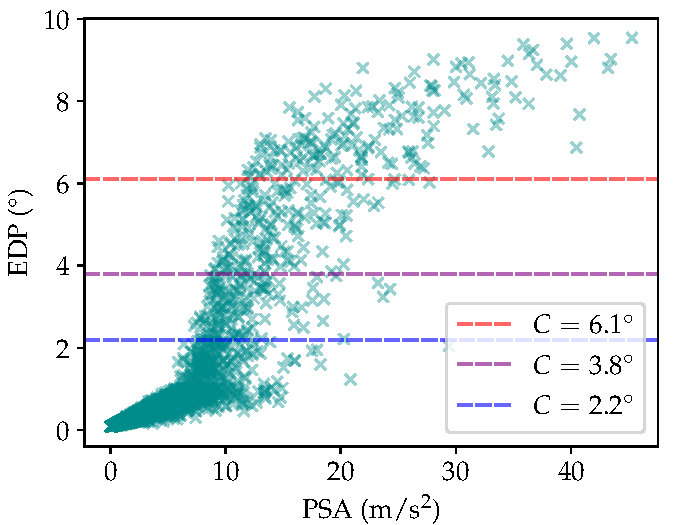
\includegraphics[width=5cm]{figures/DoE/cloud_PSA_light.pdf}\ 
    \includegraphics[width=5cm]{figures/DoE/cloud_PGA_light.pdf}%
    % 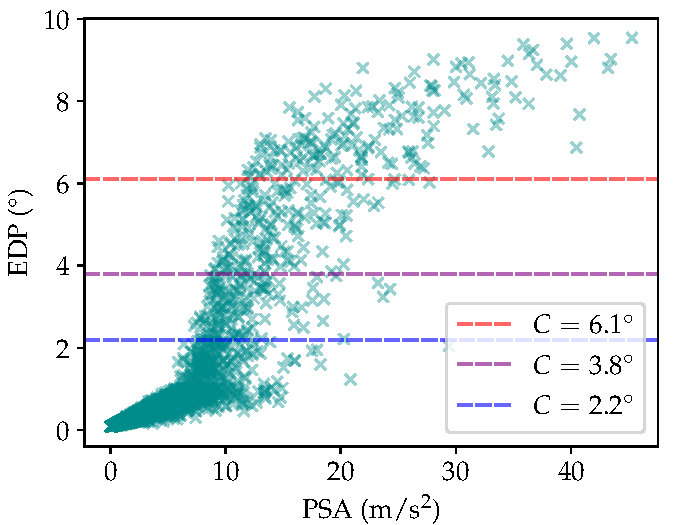
\includegraphics[width=5cm]{figures/DoE/cloud_PSA_light.pdf}%
    % \includegraphics[width=5cm]{figures/DoE/cloud_PGA_light.pdf}%
    \caption{Results of the $8\cdot10^4$ numerical simulations. Each cross is an element of the dataset (IM, EDP) where the IM is the PSA (left) and the PGA (right). Different critical rotation thresholds $C$ are plotted in dashed lines. They yield different proportions of failures in the dataset: respectively 95$\%$ (red), $90\%$ (purple) and $85\%$ (blue).}
    \label{fig:doe:scattersIMs}
    \end{figure}

    \begin{figure}[h!]
        \centering
        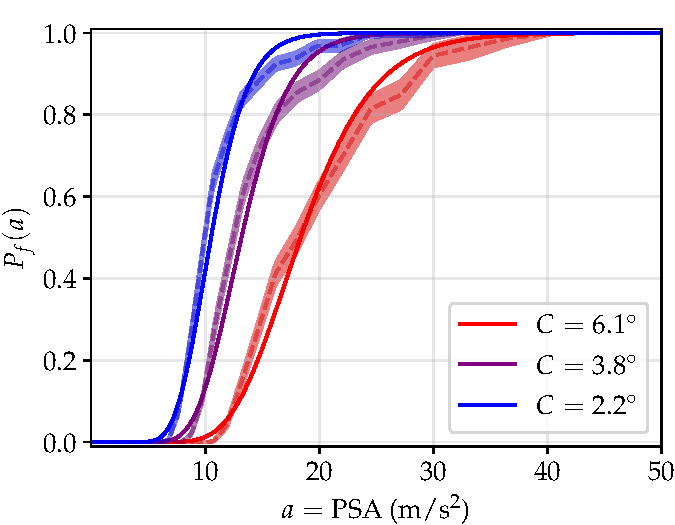
\includegraphics[width=5cm]{figures/DoE/refs_PSA.pdf}\ 
        \includegraphics[width=5cm]{figures/DoE/refs_PGA.pdf}
        \caption{{Reference non-parametric fragility curves obtained via Monte Carlo estimates (dashed lines) surrounded by their $95\%$ confidence intervals, for different critical rotation threshold $C$ with (left) the PSA and (right) the PGA as IM.} The thresholds yield different proportions of failures in the dataset: respectively $95\%$ (red), $90\%$ (purple) and $85\%$ (blue).
        For each value of $C$ are plotted (same color, solid line) the corresponding probit-lognormal MLE.}
        \label{fig:doe:reference-frags}
        \end{figure}


    \subsection{Qualitative study}



    In  \cref{fig:doe:ex-estfrag} we present examples of \emph{a posteriori} fragility curve estimations. They take the form of {$95\%$-credibility intervals. These qualitative graphs allow us to appreciate the performance of the estimation when the IMs are selected using our DoE method compared to the standard approach. In this example, the DoE was implemented by setting $\gamma=0.5$.} The same comments stay valid for any of the two IMs we have taken into account in this study ---the PSA and the PGA---, namely: 
    \begin{enumerate}
        \item[(i)] When the number of observed data is really small (20 samples), the standard method tends to provide ``vertical'' fragility curves estimates, which result in ``vertical'' credibility intervals. By verticality, understand here that the tangent of the estimated curve at the median has an infinite slope (i.e., $\beta=0$). This phenomenon is a consequence of the fact that the likelihood is degenerate in this case.
        The credibility intervals are thus tighter but strongly incorrect.
        When the DoE is implemented with the same number of samples, the phenomenon fades and the credibility intervals follow accurately the reference curve.
        \item[(ii)] When a more decent number of data are observed (80 samples), the credibility intervals given from the DoE follow quite closely the reference curve. Within the observed seismic signals, we then notice a better balance between the ones with large IMs and the ones with small IMs compared to the standard method {(see the ``red crosses'' in the figures).} The consequence is a thinner credibility interval given by the DoE method.
        %especially at the borders of the domain.
    \end{enumerate}
    
    \begin{figure}[h]
        \centering%
        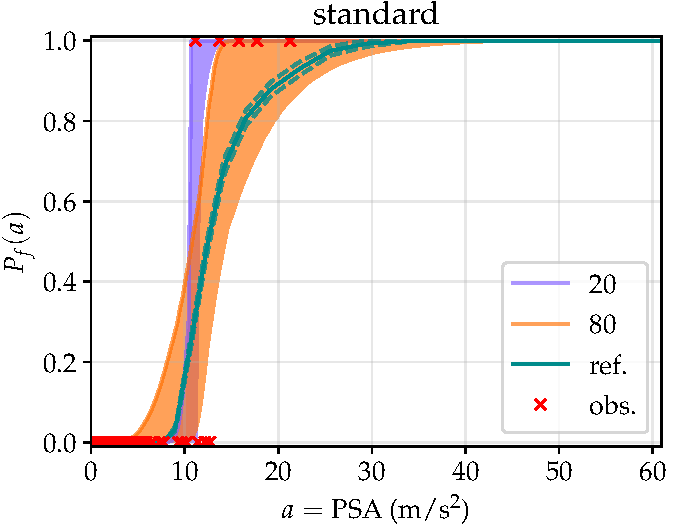
\includegraphics[width=5cm]{figures/DoE/ex_est_frag_PSA_standard_80.pdf}\ %
        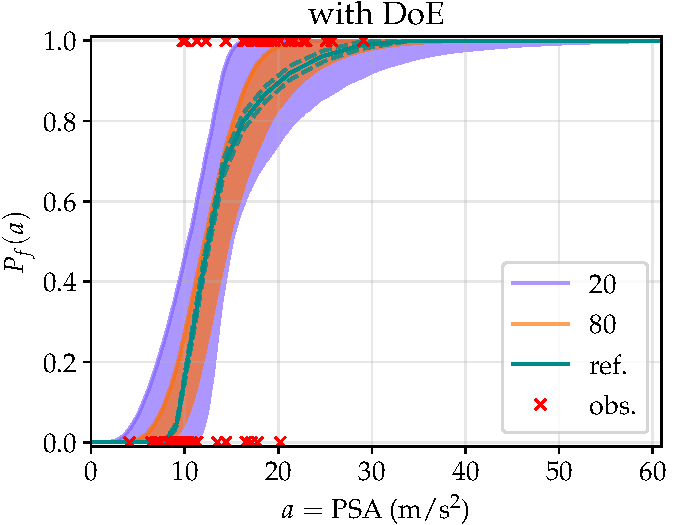
\includegraphics[width=5cm]{figures/DoE/ex_est_frag_PSA_PE_80.pdf}\\[5pt]
        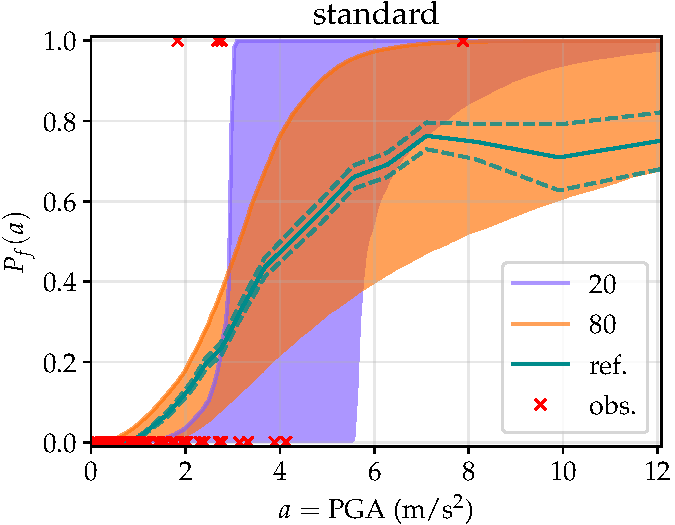
\includegraphics[width=5cm]{figures/DoE/ex_est_frag_PGA_standard_80.pdf}\ \includegraphics[width=5cm]{figures/DoE/ex_est_frag_PGA_PE_80.pdf}%
        \caption{Examples of fragility curves estimation. Top figures: the IM is the PSA; bottom figures: the IM is the PGA. Left figures: the seismic signals are chosen w.r.t. their standard distribution. Right figures: they are chosen w.r.t. our DoE strategy.
        On each figure: credibility intervals from $20$ (purple) or $80$ (orange) observations, reference fragility curves (green solid line) from Monte Carlo simulations and their {$95\%$}-confidence intervals (green dashed lines). The red crosses represent the $80$ observations.}
        \label{fig:doe:ex-estfrag}
    \end{figure}







    \subsection{Quantitative study}\label{sec:doe:appli:subsec:quantitative}



\Cref{fig:doe:errors-degen,fig:doe:errors-psa,fig:doe:errors-pga,fig:doe:variaI,fig:doe:variaP} present 
quantitative results that go beyond a single example.
Within those, 12 methods are compared:
    the standard method and the DoE methods for any $\gamma\in\{0,$ $0.1,$ $0.3,\dots,1.9\}$.
The case $\gamma=0$ is particular: in this case the prior $\pi^\ast_\gamma$ does not always satisfy the criteria for a robust \emph{a posteriori} estimation (\cref{def:doe:robust-estimation}) even though that is essential for the DoE to be implemented. Thus, $\gamma=0$ corresponds to an alteration of the DoE method:
    first, data are collected given the DoE method carried out with $\gamma=0.1$; second, the prior $\pi^\ast_{0.1}$ is replaced with $\pi^\ast_0$ to compute the estimates.
This particular treatment is carried out in order to quantify how that parametrized constraint affects the estimates.
%This particular variation of the method al

{For each of these methods, we have carried out $100$ replications of the same numerical experiment, namely: (i) generate an observed sample of $k_{\max}=250$ data items and (ii) derive for any $k=10,$ $20,\dots,k_{\max}$ the posterior distribution $p(\theta|\mbf z^k,\mbf a^k)$.
These replications provide evaluations of the mean values of the metrics defined in \cref{sec:doe:metrics}. The results are shown in  \cref{fig:doe:errors-psa} for the PSA and in  \cref{fig:doe:errors-pga} for the PGA.}

%As a first comment, we can compare the results given by the different DoE methods: the errors they give are always very close and we do not clearly distinguish a hierarchization of them w.r.t. the value of $\gamma$. This comment is valid for both the PGA and the PSA. 

\paragraph{{Overall comments on the influence of $\gamma$}}

{For both IMs, \cref{fig:doe:errors-psa,fig:doe:errors-pga} show that the discrepancies between all the DoE-based results are negligible. We do not clearly distinguish a hierarchy of these with respect to the value of $\gamma$.}
We have verified that the selected IMs by the DoE methods are actually poorly influenced by the value of $\gamma$ and that any change of performance impacted by the value of $\gamma$ is hard to distinguish. We conclude that its influence on the posterior estimation remains small. Thus, our constrained reference prior is close enough to the unconstrained ($\gamma = 0$) one and conserves its ``objectivity'' qualification.

\paragraph{Degeneracy disappearance} 

{\Cref{def:degeneracy} lists the different types of situations for which likelihood degeneracy can occur. For our case study,  \cref{fig:doe:errors-degen} presents the average number of occurrences of the three types of situations that lead to a degenerate likelihood, as a function of the number of observed samples. We observe that the DoE method clearly outperforms in reducing the degeneracy for small numbers of observations compared with the standard method (from $k\simeq 20$ in the case of the PGA, and at most $k\simeq 50$ in the case of the PSA). Echoing this observation, we notice that this probability is, in general, higher with the PSA as IM, especially when the seismic signals are selected according to the standard method.

These results must however be qualified because they arise directly from the way in which we implemented the two estimation methods ---DoE and standard---, that is to say from a large database of artificial signals (i.e., of size $8\cdot10^4$), generated {beforehand}. In \cref{app:doe:toycases}, it is indeed  mathematically demonstrated that in a well-specified case, we can define a change of variable between two fragility curves which are defined by two different values of $\theta$, all other things being equal. In other words, from the point of view of the estimation of the parameter $\theta$, all cases are equivalent if there is sufficient data in the domain of interest, that is, the domain in which the fragility curve evolves ``significantly'' from 0 to 1. As this requirement is not met in practice, especially in our case study, the estimation performances are not identical when considering two distinct IMs such as the PGA or the PSA. Thus, in the standard case, whether for the PSA or PGA, as we have considered a high failure threshold, the main cause of degeneracy comes from the fact that the observed data are of type 1, that is to say that they do not reveal any failure. The distributions are concentrated at low IM values. Then, with the PSA, as the value of $\beta$ of the fragility curve is smaller than with the PGA, while its distribution has a larger standard deviation, this favors degeneracy of type 3. To a lesser extent, this also affects the DoE method.}

\begin{figure}[h]
\centering%
\includegraphics[width=5cm]{figures/DoE/degenPSA.pdf}\ 
\includegraphics[width=5cm]{figures/DoE/degenPGA.pdf}%
\caption{Probability that a sample of size $k$ yields a degenerate likelihood, as a function of $k$. The considered IM is (left) the PSA and (right) the PGA.
The degeneracy probability without DoE (blue dashed line) is compared with the ones with DoE (dotted lines), for different values of $\gamma$. 
Two extreme values of $\gamma$ are highlighted: $\gamma=0.1$ (purple dotted line) and $\gamma=1.9$ (orange dotted line).}
\label{fig:doe:errors-degen}
\end{figure}


\paragraph{Performances with few observations} {Focusing first on the quadratic errors presented in \cref{fig:doe:errors-psa,fig:doe:errors-pga}, we show that when the number of observations $k$ is small, the outperformance of the DoE method over the standard one is clearly visible for any IM considered.}
Indeed, on the domain $k<50$, the decrease of any of the errors is faster, reaching satisfying values at $k=50$, which is consistent with the qualitative study of the previous section.
Regarding the cases where $k>50$, the behavior of the metrics differ between the case where the PSA is used and the one where it is the PGA. Globally, it is obvious that the PSA provides the best results. The consideration of this IM rather than the PGA is more relevant for this case study. {In the following paragraphs, we discuss more specifically the estimation biases for both IMs, since the quadratic error is a combination of the bias and the credibility width.}

\paragraph{Study of the bias when the IM is the PSA}
As mentioned in \cref{sec:doe:appli:subsec:present}, the PSA is the better of the two IMs in our case study. As a result, the performances of the DoE method make no doubt ( \cref{fig:doe:errors-psa}). Up to values of $k$ close to $50$, the decrease in the estimation bias is rapid towards the so-called model bias value which is materialized in the figure (see \cref{sec:doe:metrics}). This bias reflects the fact that the reference fragility curve, $P_f^{\text{ref}}$, does not correspond to an exact probit-lognormal curve as illustrated in  \cref{fig:doe:reference-frags}. Beyond a value of $k$ close to $100$, the bias stops decreasing significantly because it tends towards the model bias. From this threshold, additional observed data only make the credibility intervals thinner around the median. It is noted in this regard that the DoE method is able to provide estimates with a bias that is smaller than the so-called model bias. On average, the DoE-based estimations do not exactly match the model bias, although it is very close. This is not the case for the standard method, for which there is almost an order of magnitude difference, even with a sample size of $250$. The difference between the bias obtained on average by the DoE method and the model bias simply reflects the fact that the distributions of the data used for the estimates are not the same in the two cases. $P_f^{\text{MLE}}$ is estimated on the entire available database while the DoE methodology aims to select some of them by maximizing the criterion defined in \cref{eq:doe:index}. \Cref{app:doe:toycases} provides more insight into the DoE approach.

\begin{figure}[h]
    \centering%
    % \hspace*{-1cm}%
    \includegraphics[width=5cm]{figures/DoE/errE_PSA.pdf}\ \includegraphics[width=5cm]{figures/DoE/errB_PSA.pdf}\ \includegraphics[width=5cm]{figures/DoE/errW_PSA.pdf}%
    \caption{Average error metrics derived from numerous replications of the method, as a function of the size of the observed sample.
    In dashed blue lines: the average errors using the standard distribution of the IM surrounded by their $95\%$-confidence interval. In dotted lines: the average errors using our DoE strategy with different values of $\gamma$. They are surrounded (in red) by the maximal $95\%$-confidence intervals. Two extreme values are emphasized: $\gamma=0$ (orange) and $\gamma=1.9$ (purple).
    On the middle figure, the model square bias is plotted as a gray line.
     The IM  is the PSA here.}
    \label{fig:doe:errors-psa}
\end{figure}



\paragraph{Study of the bias when the IM is the PGA}
{As mentioned in \cref{sec:doe:appli:subsec:present}, with the PGA as IM, it is not possible to fully describe the fragility curve. We therefore have no information on its evolution beyond the maximum value of the PGA observed, at about $12$ m/s$^2$. Moreover, the discrepancies between $P_f^{\text{ref}}$ and $P_f^{\text{MLE}}$ are maximal for a PGA value of the order of $8$ m/s$^2$, whereas before this value the fit is very good.} For the strongest seismic signals at disposal, a failure of the equipment is indeed observed only around {$70\%$} of the time.

{Up to values of $k$ close to $100$, the DoE method outperforms the standard method. Beyond that, the behavior is different from that observed when the IM is the PSA and an evaluation of the performances of the DoE method is less obvious. On average, however, with the first $40$ data, the bias value obtained with the PGA is smaller than with the PSA.}

%Thus, when $k$ is above $50$, the behavior of the metrics in the case of the PGA ( \cref{fig:errors-pga}) is different {from that observed with PSA}, and an evaluation of the performances of the DoE method in this case is less obvious. Indeed, while the credibility width does not cease to decrease, we notice an increase of the bias that does not stop before $k=150$.

{In \cref{app:doe:toycases} it is shown that with the DoE method, the distribution of the selected data tends to follow a bimodal distribution equally distributed around the logarithm of the median of the fragility curve (see also  \cref{fig:doe:ex-estfrag} and the repartition of the ``red crosses''). Since knowledge of the fragility curve over a restricted domain is likely to reduce the performance of the DoE method, a thorough study of the consequences of such a restriction is proposed in \cref{app:doe:toycases}, in a case where the model bias does not exist. This study shows that the performance of the DoE method is weakly affected by this limitation. We can therefore postulate that it is the presence of a significant bias in one of the two main domains in which the DoE method selects data that is the cause of the deterioration in the method's performance for values of $k > 100$, compared to the standard approach. If we believe the results in  \cref{fig:doe:ex-estfrag}, with $80$ data, we obtain however a completely reasonable estimate, taking into account the observed bias.}

    \begin{figure}[h]
        \centering
        % \hspace*{-1cm}%
        \includegraphics[width=5cm]{figures/DoE/errE_PGA.pdf}\ \includegraphics[width=5cm]{figures/DoE/errB_PGA.pdf}\ \includegraphics[width=5cm]{figures/DoE/errW_PGA.pdf}%
        \caption{As in \cref{fig:doe:errors-psa} but here the IM  is the PSA.}
       % {Average error metrics derived from numerous replications of the method, as a function of the size of the observed sample. In dashed blue lines: the average errors using the standard distribution of the IM surrounded by their $95\%$-confidence interval. In dotted lines: the average errors using our DoE strategy with different values of $\gamma$. They are surrounded (in red) by the maximal $95\%$-confidence intervals of theirs. Two extreme values are emphasized: $\gamma=0$ (orange) and $\gamma=1.9$ (purple). On the middle figure, the model square bias is plotted as a gray line. The IM considered is the PGA here.}
        \label{fig:doe:errors-pga}
    \end{figure}




    \paragraph{{Stopping criterion}} {To the extent that an irreducible estimation bias can be expected in practice, an indication that such a bias has been reached would constitute a suitable stopping criterion for the DoE method. Since such a criterion would imply knowing, in some way, the bias itself and this is not possible with small data sizes, we suggest to study (i) the index $\cV\cI_k$ that measures the variation of the  quantity defined by \cref{eq:doe:index} that is used to select the seismic signals in the DoE method and (ii) the index $\cV\cP_k$ that measures the average evolution of the median of the fragility curve. These two quantities are defined in \cref{sec:doe:stopping_crit}. They reflect the information provided by adding a $k$-th data point. 

     \Cref{fig:doe:variaI} shows the evolutions of the average values of $\cV\cI_k$ for respectively the PSA and the PGA as IM, whereas  \cref{fig:doe:variaP} is devoted to the evolutions of $\cV\cP_k$. These two figures, once again, show that learning with the DoE method is more effective than with the standard method. $\cV\cI_k$ and $\cV\cP_k$ are slightly influenced by the change in IM. Up to values of $k$ close to $k=50$, they even indicate that with PGA, the DoE method reaches more quickly a state in which the information brought by a new data point has less impact. This result is consistent with the one mentioned in the previous paragraph, namely that with the first $40$ data, the bias value obtained with the PGA is smaller than with the PSA, with the DoE method.
    
    The practitioner can therefore use these indicators to define a stopping criterion depending on a threshold value. For instance, in our case, a threshold value set at $\cV\cI_k = 10^{-3}$ gives approximately $k_{\max} = 60$ for the PSA and $k_{\max} = 40$ for the PGA. Concerning $\cV\cP_k$, the threshold value can be set at $5 \% $. For both the PSA and the PGA, this ensures furthermore that the likelihood degeneracy probability is zero (see  \cref{fig:doe:errors-degen}). 
    Remark that, even though the number of data required to reach a given stopping criterion is smaller with the PGA than with the PSA, this does not imply that the estimate is less accurate. Indeed, for small data sizes, the degeneracy phenomenon is more likely with the PSA than with the PGA (see  \cref{fig:doe:errors-degen}). Consequently, the widths of the credibility intervals remain large for large $k$ with the PSA (see \cref{fig:doe:errors-psa,fig:doe:errors-pga}). Our approach addresses this phenomenon by reducing the degeneracy even for a few observations. In practice, however, this number remains dependent on the IM of interest (see the paragraph ``Degeneracy disappearance'').
    
    }
        
        %It is interesting to see that its evolution is consistent with the one of the bias: above a certain value of $k$, its decline slows down.
    
            %\begin{equation}
            %    \cI_{k+1}(a_{k+1}) = \EE_{z_{k+1}|\mbf a^{k+1},\mbf z^k}[D_\delta(p(\theta|\mbf z^k,\mbf a^k)||p(\theta|\mbf z^{k+1},\mbf a^{k+1}))],\quad \cV\cI_k = \frac{|\cI_{k+1}(a_{k+1})-\cI_k(a_k)|}{|\cI_k(a_k)|}
            %\end{equation}
        %(see \cref{sec:PEmethod} for the computation of $\cI$). The average value of $\cV\cI_k$ is exhibited in  \cref{fig:variaI}. It is interesting to see that its behavior is consistent with the one of the bias: above a certain threshold value of $k$, its decline slows down. It also matches the average evolution of the fragility curve $\cV\cP_k$ defined by 
           % \begin{equation}
            %    \cV\cP_k = \frac{\|m^{|\mbf z^k,\mbf a^k} - m^{|\mbf z^{k+1},\mbf a^{k+1}}\|_{L^2}}{\|m^{|\mbf z^k,\mbf a^k}\|_{L^2}};
            %\end{equation}
    
        %when the estimated fragility curves cease to clearly evolve, the average information given by new data also does. A stop criterion could be set when $\cV\cI_k$ falls below $10^{-3}$.
        %Indeed, in this case the minimal bias is close to be reached, and additional observations would result into a thinner credibility interval around this bias. It is thus pointless to pursue the experiments as the model bias is irreducible.
    
    
    \begin{figure}[h]
        \centering%
        \includegraphics[width=5cm]{figures/DoE/VariaI_PSA.pdf}\ 
        \includegraphics[width=5cm]{figures/DoE/VariaI_PGA.pdf}
        \caption{Average variations of the DoE index $\cV\cI_k$ as a function of the observed sample size $k$, using the PSA (left) and the PGA (right).}
        \label{fig:doe:variaI}
    \end{figure}
    
    
    \begin{figure}[h]
        \centering%
        \includegraphics[width=5cm]{figures/DoE/VariaP_PSA.pdf}\ 
        \includegraphics[width=5cm]{figures/DoE/VariaP_PGA.pdf}
        \caption{Average variations of the median \emph{a posteriori} fragility curve $\cV\cP_k$ as a function of the observed sample size $k$, using the PSA (left) and the PGA (right).}
        \label{fig:doe:variaP}
    \end{figure}



    \subsection{Synthesis}




    The objective of the methodology proposed in this work is to make the most of the {probit-}lognormal model. Indeed, it appears to the practitioner as a model that is both pragmatic and relevant for estimating fragility curves with a reduced number of data, judging by the abundant use made of it in the literature. The {limitation} on the number of data is essential. It comes from the fact that (i) these are expensive in absolute terms, especially %with high-fidelity numerical models, or 
with experimental tests, and (ii) the {probit-}lognormal model being likely to be biased, there is no point in feeding it with a lot of data. To achieve this goal, we proposed a methodology for planning experiments in a Bayesian framework based on the reference prior theory.

Two current IMs ---the PSA and the PGA--- were considered to study the performance of the method which was applied to an equipment from the nuclear industry. In both cases, with a small number of data ---of the order of 80---, the performance of the proposed method was much better than that of the standard one. Performance is best if the method is used with an IM that has a good level of correlation with the structural response of interest.

In order to guide the user, we also proposed two indicators that allow learning to be stopped based on quantitative information. Both criteria appeared sensitive to the change of IM and therefore to the associated potential biases. Let us add, however, that since the degeneracy phenomenon does not make the estimation optimal from the point of view of the size of the credibility interval, it is appropriate, in practice, to continue learning until a non-degenerate sample is obtained (see \cref{def:degeneracy}).



\section{Behavior of the method on toy case studies}\label{app:doe:toycases}

    \subsection{Description of the case studies}
    

    In order to gain more insight on the method, we suggest in this section a brief analysis of its behavior on case studies that are free of any bias. 
    Such case studies are purely theoretical, so that we qualify them as ``toy case studies''. Here, the observed data $(\mbf z^k,\mbf a^k)$ are perfectly generated according to the probit-lognormal statistical model presented in \cref{sec:doe:model}:
    a reference parameter $\theta^\ast=(\alpha^\ast,\beta^\ast)$ is chosen; then, from any input $a$ (that simulates a theoretical IM), an output $z\in\{0,1\}$ is generated that is equal to $1$ with probability $\Phi\left(\beta^{\ast -1}\log\frac{a}{\alpha^{\ast}}\right)$ and $0$ otherwise.
    
    The selected inputs belong to an interval $\cA=(0,a_{\text{max}}]$.
    They are picked by the {design} of experiments methodology that we present in this work with $\gamma=0.5$. Note that when implementing \cref{alg:doe:PE} in this section, there is no need to generate seismic signals from a particular value of $a$ here. Indeed, the ``experiment'' (understand here: the generation of $z$) directly results from $a$.
    Regarding the $k_0=2$ required initial value of $a$, we draw them uniformly in $\cA$.
    
    In those toy case studies, the value of $\theta^\ast$ does not matter, in the sense that two such case studies with two different value of $\theta^\ast$ would be equivalent up to a translation and a dilatation w.r.t. $\log a$ (see \cref{app:equiv-toy} for a proof of this statement).
    
    In this section, we present three different toy case studies. They are all implemented using the same value of $\theta^\ast$. 
    They differ from the different domains $\cA$ that are selected for them.
    The limits $a_{\text{max}}$ of these domains are chosen to simulate an upper bound 
    on the possible IM that can result from a generated seismic signal.
    They are selected to match a quantile of the reference fragility curve: if $q\in[0,1]$ one can derive $a_q$ such that $P^{\text{ref}}_f(a_q):=\Phi\left(\beta^{\ast -1}\log\frac{a_q}{\alpha^{\ast}}\right)=q$, i.e.
        \begin{equation}
            a_q = \exp\left( \beta^\ast t_q+\log\alpha^\ast \right),
        \end{equation}
    where $t_q$ represents the $q$-quantile of a standard Gaussian distribution.
    
    The three toy case studies implemented in this work result from defining $a_{\text{max}}=a_q$ with:
    \begin{itemize}
        \item $q\simeq1$ (actually $q=1-10^{-3}$), to represent a case where no upper bound (or a very high one regarding the fragility curve) limits the generation of IMs. %This case could correspond to the scale of the case study of \cref{sec:application} when the IM is the PSA (however, there are no bias here).
        \item $q=0.9$.
        \item $q=0.8$.
    \end{itemize}
    The reference fragility curve of each of these toy case studies are plotted in  \cref{fig:histograms_toy} (green solid lines) for each of the values of $q$ aforementioned, and for $\theta^\ast=(3,0.3)$. 
    %On  \cref{fig:ex_est_toys} are presented examples of credibility interval estimation.
    
    
    
    
    
    \subsection{Results}
    
    The design of experiments method has been run a hundred times for each case study. Each time, we have stopped the algorithm after it reached a number of $250$ observed samples.
    The last $100$ of these generated IMs have been kept for each run. As we have carried out $100$ runs, they constitute a sample of $10^4$ values of IMs selected by the experimental design.
    %To focus on the distribution of the selected IMs by the method, we kept for each run the 100 last ones. Thus, we have at our disposal a sample of $10^4$ values of IMs selected by the planning of experiments algorithm at least 150 steps after its initialization, for each case study. 
    The three empirical distributions of these samples resulting from the three values of $q$ are compared in  \cref{fig:histograms_toy}.
    
    % As one c
    
    When the method is not limited by any upper bound for the choice of IMs (i.e. case $q=1$), 
    the logarithms of the selected ones are symmetrically distributed around $\log\alpha^\ast$. This comment was expected as in the statistical modeling, $\log a$ is mathematically symmetric around $\log\alpha^\ast$ as well.
    
    The bimodal appearance of the distribution supports the ``well-posedness'' of the method. Indeed, in a case where the result is deterministic, the knowledge of the evaluation of the curve in two points is enough to recover its parameter $\theta^\ast$. Thus, it makes sense that the optimal distribution of the IM for estimating the whole fragility curve is to retrieve a proper estimation of its evaluation in two zones of the domain.
    A simple calculation is done in \cref{sec:au-maths-calc} to suggest possible appropriate centers of the zones. 
    {These are called $a^u_1$ and $a^u_2$ and are appropriate in the sense that they are the points that most help distinguish a stochastic fragility curve from a deterministic one.}
    %two different fragility curves.}
    %they are optimal in the sense that they are the {points} where the estimated value of the fragility curve is expected to be the worse when it is compared with the reference. {!!  je vais y réflechir mais cette phrase n'est pas très clair à mon sens !!}
    In  \cref{fig:histograms_toy}, their values are emphasized (dashed pink line). They are clearly close from the actual modes of the empirical distribution of the IM in the case $q=1$.
    
    
    In the cases where the IM selection is limited ($q<1$), the method has been designed to select $a_{\text{max}}$ when the index tended to be maximized by a value which is higher.
    We notice that the method seems to target the same ideal domain as when $q=1$: converging to a bimodal strategy with modes around optimal domains. The method is robust: for two given $q_1$, $q_2$ and their $a_{\text{max}}^1$, $a_{\text{max}}^2$, associated to two toy case studies, around the same proportion of IMs are selected below $a$ for any $a\leq\min(a_{\text{max}}^1, a_{\text{max}}^2)$ in the two cases.
    This results in numerously selected IMs equaling $a_{\text{max}}$ when it is falls close to the second expected mode of the optimal distribution.
    
    In  \cref{fig:metrics-toy}-left, we compare the average square bias
    resulting from the 100 replications of the three case studies.
    Their difference is hard to distinguish, so that the robustness of the method is supported: even when the limit among the available IMs strongly cuts the reference fragility curve, the distribution of the selected ones still provides an accurate estimation.
    However, a close look allows to notice the expected loss of performance induced by such limit: the smaller is $q$, the larger is the bias.
    
    Regarding the other metrics exposed in  \cref{fig:metrics-toy}, namely the indices $\cV\cI_k$ and $\cV\cP_k$, it is interesting to notice that their behaviors are comparable with the ones of the real case study. In particular, $\cV\cI_k$ reaches the threshold $10^{-3}$ for a similar number of observations (around $50$) in any of the case studies implemented in this work (real ones as well as toy ones).
    As a matter of fact, the index sequentially measures the quantity of information brought by the next seismic signal selected by the DoE. Thus, the stability of that quantity between case studies supports the robustness of our approach in selecting IMs to inform the estimate and enhance the learning.
    However, the indices $\cV\cP_k$ are smaller for toy case studies. Without any model bias, the estimates reach more quickly the reference (see the average bias in  \cref{fig:metrics-toy}-left), so that they evolve less.
    
    %{
    %Finally, this section helps to clarify the limit of a comparison between the results obtained with two different IMs in \cref{sec:quantitative-study}. 
    %Indeed, a clear difference between the cases where the IM is the PGA and the one where it is the PSA is the difference of scale of the reference fragility curve between those two. When it is the PGA, the fragility curve is cut far before being close to one, when it equals around $0.8$ or $0.9$. 
    %Thus, up to the model bias, an analogy is possible between the real case studies and the toy ones, where the piping system with PSA corresponds to our toy case study with $q=1$, and the piping system with PGA corresponds to $q=0.8$ or $q=0.9$. 
    %The results elucidated in this section prove that this difference has little influence on the estimates by deteriorating slightly the square bias. This deterioration remains however negligible in front of the model biases of the real case studies.}
    
    {Finally, this section helps to clarify the results obtained with the two IMs that are the PSA and the PGA in \cref{sec:doe:appli:subsec:quantitative}. The main difference between them is that with the PGA it is not possible to completely describe the fragility curve. With the PGA, the maximum value of its probit-lognormal estimate is approximately $0.8$ but does not reach $1$ as with the PSA. If we ignore the bias, this means that the case $q=1$ is similar to the situation where the PSA is used as IM, while the cases  $q=0.8$ and $q=0.9$ are similar to the situation where the PGA is used. All things being equal, this study shows that the performance of the DoE method is weakly affected by a restricted learning domain. It is then likely that the presence of a significant bias in one of the two main domains in which the DoE method selects data is the cause of its performance degradation.}
    
    %
    %As proven by the results elucidated in this section, a short upper bound on the IM influences the estimation with a higher bias. This coincides with comments done in \cref{sec:quantitative-study}. However, as precised in the above paragraph, the impact of this phenomenon on the bias remains really little. That confirms that in the case of the piping system, the variations of the bias when the PGA is used as IM resorts to multiple factors. {!! il me semble qu'il faudrait reprendre ce dernier paragraphe car il manque de clarté, même si à demi-mot on comprend ce que tu veux dire !!}
    
    \begin{figure}[h]
            \centering%
            % \makebox[0pt][c]{%}
            %\hspace*{-2cm}
            \includegraphics[width=5cm]{figures/DoE/toy_A_1.pdf}\ 
            \includegraphics[width=5cm]{figures/DoE/toy_A_09.pdf}\ 
            \includegraphics[width=5cm]{figures/DoE/toy_A_08.pdf}%}%
            \caption{For each of the three toy case studies: the distribution of the 100 last selected IM by the method (red histograms) along with the associated reference fragility curve (green) of the toy case study, which is cut at a certain quantile $q$ in each figure. The median of the reference (solid blue) and the values $a^u_{1}$, $a^u_{2}$ (dashed pink) are emphasized.}
            \label{fig:histograms_toy}
        \end{figure}
    
    % \begin{figure*}
    %         \centering%
    %         \makebox[0pt][c]{%}
    %         %\hspace*{-2cm}
    %         \includegraphics[width=5cm]{figures/ex_toy_1.pdf}\ 
    %         \includegraphics[width=5cm]{figures/ex_toy_09.pdf}\ 
    %         \includegraphics[width=5cm]{figures/ex_toy_08.pdf}}%
    %         \caption{Examples of credibility intervals estimation for each of the three toy case studies. On each case, 80 observed data (red crosses) have been selected via the DoE method. The \emph{a posteriori} credibility intervals are derived for 20 of the observed samples (in purple), and for the 80 ones (in orange). On each case, the reference (green) is cut from $a_{\max}$. Note that any comparison is limited because the distribution of selected data remains volatile (especially for 20 samples).}
    %         \label{fig:ex_est_toys}
    %     \end{figure*}
    
    
        % \begin{figure}
        %     \centering
        %     \includegraphics[width=5cm]{figures/toy_bias.pdf}
        %     \caption{Average square bias of the three toy case studies as a function of the number of observations.}
        %     \label{fig:bias-toy}
        % \end{figure}
    
    \begin{figure}[h]
        \centering%
        % \makebox[0pt][c]{%}
        \includegraphics[width=5cm]{figures/DoE/toy_bias_log.pdf}%
        \includegraphics[width=5cm]{figures/DoE/toyVI.pdf}%
        \includegraphics[width=5cm]{figures/DoE/toyVP.pdf}%}%
        \caption{Left figure: average square bias of the three toy case studies as a function of the number of observations. Middle figure: index $\cV\cI_k$ for the three toy case studies as a function of the number of observations. Right figure: index $\cV\cP_k$ for the three toy case studies as a function of the number of observations.}
        \label{fig:metrics-toy}
    \end{figure}
    
    
    
    \subsection{Simple suggestion of a domain where IMs should be theoretically selected}\label{sec:au-maths-calc}
    
    
    
    
    In this section we suggest a criterion that gives insight on a domain where the
    fragility curve should be evaluated in order to optimize the estimation.
    {For this purpose, we study the quantity $\EE[ |P^{\text{ref}}_f(a)-P_f(a)| ]$ as a function of $a$, where $P^{\text{ref}}_f(a)$ represents a deterministic fragility curve and $P_f(a)$ denotes a stochastic estimate.
    If $a^\ast$ is a maximal argument of this quantity, it would 
    be the one that helps the most distinguishing the two curves.}
    %represent the best point to compare the fragility curves in order to discriminate them
    %A maximal argument of this quantity would 
    %give points within which the distinction between }
    %be a value of the IM within which the expected estimation is the worse, i.e. an input where there is a lack of information. 
    %Additional evaluations of the output in this point should thus enhance the most the evaluation.
    
    
    
    
    
    For this theoretical study, we assume to be in the settings of the toy case studies defined in the previous subsection, i.e. $P^{\text{ref}}_f(a)=\Phi\left(\beta^{\ast -1}\log\frac{a}{\alpha^{\ast}}\right)$ for a couple $(\alpha^\ast,\beta^\ast)$.
    We derive
        \begin{align}\nonumber
            &\frac{d}{da}\EE|P^{\text{ref}}_f(a)-P_f(a)|\\ &= \frac{1}{a\sqrt{2\pi}}\int_\Theta \left[\frac{1}{\beta^\ast}\exp\left(-\frac{(\log a-\log\alpha^\ast)^2}{2\beta^{\ast 2}}\right)-\frac{1}{\beta} \exp\left(-\frac{(\log a-\log\alpha)^2}{2\beta^2}\right)\right] p_{\alpha,\beta}(\alpha,\beta)d\alpha d\beta. \label{eq:derive-P-EP}   
        \end{align}
    To pursue, we can assume that $(\alpha,\beta)$ follows an inverse-gamma-normal distribution. This class covers a wide range of different distributions and is conjugate with a normal distribution, so that the following computation is tractable. Additionally, the probit-lognormal modeling of the fragility curve is equivalent to assume that there exists a latent variable $Y$ that is linearly correlated with the input: $Y=\log A +\cN(-\log\alpha^\ast,\beta^\ast)$. Considering this latent modeling, we can prove that both the reference prior and the posterior distribution of $\alpha,\beta$ belong to the class of inverse-gamma-normal ones (see \cref{app:chap:ESAIM}).
        %
    % If we consider the least informative case for $p_{\alpha,\beta}$ where $\log\alpha$ has an uniform distribution on $\RR$, then the left-hand term of \cref{eq:derive-P-EP}) is equal to
    %     \begin{equation}
    %         \frac{1}{\sqrt{2\pi}}\frac{1}{a\beta^\ast}\exp\left(-\frac{(\log a-\log\alpha^\ast)^2}{2\beta^{\ast2}}\right) - \frac{1}{a},
    %     \end{equation}
    % which equals $0$ if and only if $a=a^u_1$ or $a=a^u_2$ where the latter are defined by 
    %     \begin{equation}
    %         a^u_{1,2} = \alpha^\ast\exp\left( \pm\sqrt{2}\beta^\ast \left|\log\beta^\ast\sqrt{2\pi} \right|^{1/2} \right).
    %     \end{equation}
    %
    % In a more general case than the least informative one, we can assume $(\alpha,\beta)$ to follow an inverse-gamma-lognormal distribution. Indeed, such a distribution (i) remains general enough to cover a lot of possible distributions, (ii) is conjugate with a normal distribution so that the computation stays tractable. Moreover, the probit-lognormal modeling is equivalent to assume that a latent variable $Y$ is linearly correlated with the input : $Y=\log a+\cN(-\log\alpha^\ast,\beta^2)$, $Z$ being equal to $\indic_{Y>0}$.
    % Considering this latent modeling, both the reference prior and the posterior distribution of $\alpha,\beta$ belong to inverse-gamma-lognormal ones \cite{VanBiesbroeckESAIMProcS}. 
    The inverse-gamma-lognormal distribution is defined by its density:
    \begin{align}
        p_{\alpha,\beta}(\alpha,\beta) &= K(c,d,\tau,\zeta)\left(\frac{1}{\beta^2}\right)^{c+1/2}\exp\left(-\frac{d}{\beta^2}\right)\exp\left(-\tau\frac{(\log\alpha-\zeta)^2}{2\beta^2}\right),\nonumber\\
        \text{with}\quad K(c,d,\tau,\zeta) &=\frac{d^c\sqrt{\tau}}{\Gamma(c)\sqrt{2\pi}},
    \end{align}
    where $c>0$, $d>0$, $\tau>0$ and $\zeta\in\RR$ are the parameters of the distribution. %Note that the non-informative settings treated previously corresponds to the limit case where $\tau=0$.
    
    Thus, the right-hand term in  \cref{eq:derive-P-EP} becomes:
    \begin{equation}
        \frac{1}{\sqrt{2\pi}}\frac{1}{a\beta^\ast}\exp\left(-\frac{(\log a-\log\alpha^\ast)^2}{2\beta^{\ast2}}\right) - \frac{d^c}{(d+\frac{\tau}{2\tau+2}(\zeta-\log a)^2)^{c+1/2}}\frac{\sqrt{\tau}}{\sqrt{\tau+1}}\frac{\Gamma(c+\frac{1}{2})}{\Gamma(c)}\frac{1}{a\sqrt{2\pi}},
    \end{equation}
    so that it equals $0$ if and only if $a$ verifies:
    \begin{equation}\label{eq:equality-au}
        |\zeta-\log a|\frac{e^{1/2}}{\beta^\ast}\exp\left(-\frac{(\log a-\log\alpha^\ast)^2}{2\beta^{\ast2}}\right) = \frac{d^c|\zeta-\log a|e^{1/2} }{(d+\frac{\tau}{2\tau+2}(\zeta-\log a)^2)^{c+1/2}}\frac{\sqrt{\tau}}{\sqrt{\tau+1}}\frac{\Gamma(c+\frac{1}{2})}{\Gamma(c)}.
    \end{equation}
    Given the derivations conducted in \cref{app:additionalmaths}, the right-hand term of the above equation tends to 1 when information is provided by observed data to the posterior. In this case and if $\zeta=\log\alpha^\ast$  the equation leads to $a=a^u_1$ or $a=a^u_2$ where $a^u_1$, $a^u_2$ are defined by
        \begin{equation}
            a^u_{1,2} = \alpha^\ast\exp\left(\pm\beta^\ast\right).
        \end{equation}
    
    These values are built on a criterion that has a concrete and practical sense. However, they remain purely theoretical as they depend on the exact value of $\theta^\ast$.
    
    
    
    % Else, it 
    
    
    
    
    % % with the right hand term of 
    % the derivation conducted in Section   states that the right-hand term of the above equation is bounded between 
    
    
    \subsection{Additional mathematical derivations}\label{app:additionalmaths}
    
        The goal of this section is to study the domain of the right-hand term of \cref{eq:equality-au}, especially in the ``worst'' cases (the distribution is very-informative or non-informative).
        We rely on the following lemmas:
        \begin{lem}\label{lem:app-ineqG}
            For any $c>0$, $\displaystyle{\frac{\Gamma\left(c+\frac{1}{2}\right)}{\Gamma(c)}<\sqrt{c}}$. Also, $\displaystyle{
                \lim_{c\rightarrow\infty}\frac{\Gamma\left(c+\frac{1}{2}\right)}{\Gamma(c)\sqrt{c}}=1.
                }$
        \end{lem}
        \begin{proof}
            The first statement is a direct consequence of Gautschi's inequality \citep{gautschi_elementary_1959}: for any $c>0$, $s\in(0,1)$,
                \begin{equation}
                    c^{1-s}<\frac{\Gamma(c+1)}{\Gamma(c+s)}<(c+1)^{1-s}.
                \end{equation}
            Fixing $s=1/2$ and using the identity $\Gamma(c+1)=c\Gamma(c)$ leads to the result.
    
            For the second statement, we can rely on Stirling's formula \citep{davis_leonhard_1959} that yields:
                \begin{equation}
                    \Gamma(c+t) \equi{c\rightarrow\infty} \Gamma(c)c^t
                \end{equation}
            for any $t\in\CC$.
        \end{proof}
        
        \begin{lem}\label{lem:app-ineqdcf}
            Let $f>0$, for any $d,c>0$ we define:
            \begin{equation}
                g(c,d) = \frac{\sqrt{c}}{(d+f)^{1/2}}\left(\frac{d}{d+f}\right)^c, \quad h(d) = \frac{1}{2}\log\left(1+\frac{f}{d}\right)^{-1}.
            \end{equation}
            Thus, for any $c,d>0$, $g(c,d)<(2ef)^{-1/2}$, and $\displaystyle{\lim_{d\rightarrow\infty}g(h(d),d)=(2ef)^{-1/2}}.$
        \end{lem}
        \begin{proof}
            Let us differentiate $g$ w.r.t. $c$:
            \begin{equation}
                \frac{\partial}{\partial c}g(c,d) = (d+f)^{-1/2}\left(\frac{d}{d+f}\right)^c\left[\sqrt{c}\log\left(\frac{d}{d+f}  \right)+\frac{1}{2\sqrt{c}}\right].
            \end{equation}
            The above quantity is decreasing w.r.t. $c$ and equals $0$ when $c=h(d)$.
            We deduce that for any $d>0$, 
            \begin{equation}\label{eq:lem:ghdd}
                g(c,d)<g(h(d),d) = \frac{(2e)^{-1/2}}{(d+f)^{1/2}}\log\left(1+\frac{f}{d}\right)^{-1/2}.
            \end{equation}
            
            Now, let us briefly study the function $v(t)=(1+t^{-1})\log(1+t)$ for $t>0$.
            Firstly, $\log(1+t)\equi{t\rightarrow0}t$ so that $v(t)\conv{t\rightarrow0}1$. Secondly, $v'(t) = \frac{1}{t}-\frac{1}{t^2}\log(1+t)$, which is positive for any $t>0$, and tends to $\frac{1}{2}$ when $t=0$. Therefore, $v(t)>v(0)=1$ for any $t>0$. 
    
            Going back to \cref{eq:lem:ghdd}, we can write $g(h(d),d)=(2ef)^{-1/2}v(f/d)^{-1/2}$ to obtain that
                \begin{equation}
                    g(c,d) <(2ef)^{-1/2}\quad\text{and} \quad \lim_{d\rightarrow\infty}g(h(d),d)=(2ef)^{-1/2}.
                \end{equation}
        \end{proof}
    
    The result of \cref{lem:app-ineqdcf} with $f=\frac{1}{2}\frac{\tau}{\tau+1}(\log a-\zeta)^2$ lets us write the following inequality:
        \begin{equation}
            \frac{d^c\sqrt{c}}{(d+\frac{\tau}{2\tau+2}(\zeta-\log a)^2 )^{c+1/2}}\frac{\sqrt{\tau}}{\sqrt{\tau +1}} < \frac{e^{-1/2}}{|\zeta-\log a|},
        \end{equation}
        this upper-bound being reached at the border of the domain. Combining this statement with \cref{lem:app-ineqG}, we obtain: 
            \begin{equation}
                \frac{d^c|\zeta-\log a|e^{1/2}}{(d+\frac{\tau}{2\tau+2}(\zeta-\log a)^2 )^{c+1/2}}\frac{\sqrt{\tau}}{\sqrt{\tau +1}}\frac{\Gamma(c+\frac{1}{2})}{\Gamma(c)} < 1,    
            \end{equation}
        this upper-bound being reached at the border of the domain.
    
        Additionally, the left-hand term of the above equation is non-negative and tends to $0$ for some extreme values of the parameters.
        Therefore, there exist two extreme cases for the resolution of \cref{eq:equality-au}: when its right-hand term equals $0$ and when it equals $1$. The former corresponds to the limit case where the solution is $a=\pm\infty$ or $a=\zeta$, with $a=\pm\infty$ minimizing the quantity of interest. 
        The latter corresponds to the limit case where the solution verifies
            \begin{equation}
                \frac{|\zeta-\log a|^2}{\beta^{\ast2}} = \exp\left( \frac{|\log\alpha^\ast-\log a|^2}{\beta^{\ast2}} -1\right).
            \end{equation}
        The solutions of the above equation when $\zeta =\log\alpha^\ast$ are $a=\alpha^\ast\exp\left(\pm\beta^\ast\right).$
        They correspond to the limit case when the distribution $p_{\alpha,\beta}$ becomes informed and unbiased. 
        If the model is appropriately specified, that should be the fate of the posterior distribution: the posterior tends to match a normal distribution with mean $\theta^\ast$ and variance $\frac{1}{k}\cF^{-1}(\theta^\ast)$ where $\cF$ refers to the Fisher information matrix \citep{van_der_vaart_asymptotic_1992}.
    
        
    
    
    
    
    \subsection{Equivalence between toy case studies}\label{app:equiv-toy}
    
        Let us consider two different toy case studies. They can differ by their reference parameters $\theta_1^\ast$, $\theta_2^\ast$ and their IMs $a_1$, $a_2$, which are defined in the domains $\cA_1$, $\cA_2$.
        We suppose that the bounds of $\cA_1$ and $\cA_2$ are defined to match the same quantiles of the reference fragility curves: $\cA_1=(c_1^1,c_1^2)$, $\cA_2=(c_2^1,c_2^1)$ with $P^{\mathrm{ref}}_1(c_1^1)=P^{\mathrm{ref}}_2(c_2^1)$ and $P^{\mathrm{ref}}_1(c_1^2)=P^{\mathrm{ref}}_2(c_2^2)$, where $P^{\mathrm{ref}}_1$ (reps. $P^{\mathrm{ref}}_2$) denotes the reference fragility curves given by $\theta_1^\ast$ (resp. $\theta^\ast_2$).
    
        Therefore, if we introduce $\tilde a$ that defines the value of a new IM on the second toy case study, which verifies
        \begin{equation}
            \log\tilde a = \frac{\log c_1^2-\log c_1^1}{\log c_2^2-\log c_2^1}\log\frac{a_2}{c_2^1} + \log c_1^1,
        \end{equation}
        we obtain that $\tilde a$ lives in the domain $\tilde\cA=\cA_1$. Given this new IM, the reference fragility curve of the second case study can be re-defined as a function of $\tilde a$:
            \begin{equation}
                \tilde P^{\mathrm{ref}}_2(\tilde a) = \Phi\left(\beta^{\ast-1}_2\left[\frac{\log c_2^2-\log c_2^1}{\log c_1^2-\log c_1^1}\left(\log\tilde a-\log c_1^1\right)+\log c_1^1-\log\alpha^\ast_2 \right]\right) = \Phi\left(\tilde\beta^{\ast-1}_2\log\frac{\tilde a}{\tilde\alpha^\ast_2}\right),
            \end{equation}
        for a certain $\tilde\theta^\ast_2 = (\tilde\alpha_2^\ast,\tilde\beta_2^\ast)$.
        We have $\tilde P^{\mathrm{ref}}_2(c_1^1)=P^{\mathrm{ref}}_2(c_2^1)=P^{\mathrm{ref}}_1(c_1^1)$ and $\tilde P^{\mathrm{ref}}_2(c_1^2)=P^{\mathrm{ref}}_2(c_2^2)=P^{\mathrm{ref}}_1(c_1^2)$, thus, as the parameter $\theta$ defines uniquely a probit-lognormal fragility curve, $\theta_1=\tilde\theta_2$.
    
        As a conclusion, given a rescaling of the IM, the two case studies are equivalent.
    
        
    
% \section{Application of the method on the piping system}


% \subsection{Case study description as a reminder}


% \subsection{}


\section{Conclusion}\label{sec:doe:conclusion}





% In some sense, this chapter can be seen as an ``ultimate'' application 





% Assessing 
% the estimation of probit-lognormal seismic fragility curves in a Bayesian framework
% amounts to 


When we seek to estimate seismic fragility curves with limited data, 
the information conveyed by any sources ---the prior, the observations, the model--- hugely influence the quality of the estimates.


%the seismic fragility of structures and components 
%when few binary data are available ---i.e., less than 100--- is a challenging task. To do this, it is often necessary to introduce some simplifying assumptions. 
%The simplest and most widespread assumption assumes a linear correlation between the logarithm of the structural response of interest and the logarithm of the IM of interest. However, recent studies have shown that this assumption should be avoided because of the unavoidable bias it may introduce, which can greatly affect the estimation. Another preferred solution in the literature, 
%A standard solution found in the literature
%is to use a parametric model of the fragility curves such as the probit-lognormal model. This is the choice that was made in this work.

%Several methods can be implemented to estimate the model parameters. Th the use of Bayesian methods which are known to be regularizing. The question of the choice of the prior is then significant because it inevitably impacts all the resulting estimates, especially with small data sizes.

In this work, we considered as in the previous chapters the probit-lognormal model, and had thus to acknowledge its irreducible bias compared with the actual reference fragility curves of the studied component.
%limited

Regarding \emph{a priori} information, we 
relied on the reference prior theory in order to define the prior. This framework makes it possible to define a so-called objective prior in the sense that it favors the information brought by the data to the estimates. Because the
most objective prior according to the theory does not
tackle degenerate likelihoods and issues improper posteriors, we derived a slightly modified reference prior, more efficient and more robust.
However, one has to note that this prior is slightly more informative than the original reference prior.

To optimize data allocation, we have proposed a design of experiments strategy that also inherits from the reference prior theory, i.e., that is based on information theory. Given a large database of synthetic seismic signals, the proposed strategy intends to sequentially select the synthetic signals with which to perform the calculations or the tests, in order to optimally estimate ---by minimizing their number--- the probit-lognormal estimations of fragility curves.

We proved that our method is robust and
that \emph{a priori} information incorporated through the modified prior is quickly negligible in front of the information brought by the data when they are selected by the experimental design.
Compared to a standard approach that aims to select seismic signals in their initial distribution, considering the Jeffreys prior, we have shown the superiority of our method. It allows reaching more quickly ---i.e., with a limited number of data--- a small estimation bias with a small credibility interval, while reducing the phenomenon of degeneracy. The proposed methodology therefore makes the most of the log-normal model. Since estimation biases can be expected in practice, it is recommended to use the method with few data (i.e., less than 100). To this end, we propose two stopping criteria that reflect the information provided by any additional data.
\newpage
% Finally, let us note that the DoE methodology was applied here within the framework of the reference prior theory because the authors believe that the objectivity of the prior is essential for fragility analyses. However, the DoE methodology can be applied with any prior that is proper.






\part{Conclusion \& perspectives}\label{part:conclusion}


\appendix
\part*{Appendix}\label{part:appendix}
% \addcontentsline{toc}{part}{Appendix}

%\renewcommand{\thechapter}{\Alph{chapter}}

\chapter{Influence of the IM choice on fragility curves estimated using a reference prior}\label{app:chap:uncecomp}
%in a Bayesian framework based on reference prior



\begin{abstract}[\hspace*{-10pt}]
    This appendix is a postprint of the published work: \fullcite{van_biesbroeck_influence_2023}  % Ce chapitre reprend principalement les travaux publiés dans: 
\end{abstract}

\begin{abstract}
    abstract
\end{abstract}

\minitoc



% \section*{Foreword}
% \addcontentsline{toc}{section}{Foreword}


\section{Introduction}


Seismic fragility curves are key quantities of the Seismic Probabilistic Risk Assessment (SPRA) studies carried out on mechanical structures. They were introduced in the 1980s for safety studies of nuclear facilities (see e.g.
\cite{kennedy_probabilistic_1980,kennedy_seismic_1984,park_survey_1998,kennedy_risk_1999,cornell_hazard_2004}).
%\cite{Kennedy1980,KENNEDY198447, PARK1998, KENNEDY1999, Cornell2004}). 
They express the probability of failure of the mechanical structure conditional to a scalar value derived from the seismic ground motions ---called Intensity Measure (IM)--- such as the Peak Ground Acceleration (PGA) or the Pseudo-Spectral Acceleration (PSA) for a fixed frequency and damping. In practice, various data sources can be exploited to estimate fragility curves, namely: expert judgments supported by test data \citep{kennedy_probabilistic_1980,kennedy_seismic_1984,park_survey_1998,zentner_fragility_2017}, experimental data \citep{park_survey_1998,gardoni_probabilistic_2002,choe_closed-form_2007}, results of damage collected on existing structures that have been subjected to an earthquake \citep{shinozuka_statistical_2000,lallemant_statistical_2015,straub_improved_2008}  and analytical results given by more or less refined numerical models using artificial or real seismic excitations (see e.g. \cite{zentner_numerical_2010,wang_influence_2020,mandal_seismic_2016,wang_seismic_2018,wang_bayesian_2018,zhao_seismic_2020}). Parametric fragility curves were historically introduced in the SPRA framework because their estimates require small sample sizes. The log-normal model has since become the most widely used model (see e.g. \cite{shinozuka_statistical_2000,lallemant_statistical_2015,straub_improved_2008,zentner_numerical_2010,wang_influence_2020,mandal_seismic_2016,wang_bayesian_2018,wang_seismic_2018,zhao_seismic_2020,ellingwood_earthquake_2001,kim_development_2004,mai_seismic_2017,trevlopoulos_parametric_2019,katayama_bayesian-estimation-based_2021}).
Several strategies can be implemented to fit the median, $\alpha$, and the log standard deviation, $\beta$, of the model. Some of them are compared in \cite{lallemant_statistical_2015} highlighting advantages and disadvantages.
When the data is binary ---i.e., when it indicates failure or not--- \citet{lallemant_statistical_2015} recommended maximum likelihood estimation (MLE). When the data are independent, the bootstrap technique can be used to obtain confidence intervals relating to the size of the sample considered (e.g. \cite{shinozuka_statistical_2000,zentner_numerical_2010,wang_influence_2020}). 

Among the various other methods not mentioned in this short introduction, the Bayesian framework has recently become increasingly popular in seismic fragility analysis (see e.g. \cite{gardoni_probabilistic_2002,wang_seismic_2018,katayama_bayesian-estimation-based_2021,koutsourelakis_assessing_2010,damblin_approche_2014,tadinada_structural_2017,kwag_computationally_2018,jeon_parameterized_2019,tabandeh_physics-based_2020}). 
It actually allows to solve irregularity issues encountered in the estimation of the parametric fragility curves. MLE-based methods can indeed lead to unrealistic or degenerate fragility curves such as unit step functions when the data availability is sparse. Those problems are especially encountered when resorting to complex and detailed modeling due to the calculation burden or when dealing with tests performed on shaking tables, etc. In earthquake engineering, Bayesian inference is often used to update log-normal fragility curves obtained beforehand by various approaches, by assuming independent distributions for the prior values of $\alpha$ and $\beta$ such as log-normal distributions (see e.g. \cite{tadinada_structural_2017,kwag_computationally_2018,wang_seismic_2018,katayama_bayesian-estimation-based_2021,straub_improved_2008}).

This work follows the one presented in \cref{chap:prem}, which deals with Bayesian problems in which only few binary data are available. Using the reference prior theory as a support, the authors have proposed an objective approach to choose the prior and to simulate a posteriori fragility curves. This approach led to the Jeffreys prior and the authors have shown the robustness and advantages of the Jeffreys prior in terms of regularization (no degenerate estimations) and stability (no outliers of the parameters) for fragility curves estimation. Since this prior depends only on the characteristics of the ground motion ---the distribution of the IM of interest--- its calculation is then suitable for any equipment of an industrial installation subjected to the same seismic hazard. So, in this work, we are interested in the influence of the choice of the IM ---PGA vs. PSA--- on the convergence of the estimates, for a given magnitude (M) - source-to-site distance (R) scenario and a given mechanical structure.

The paper is organized as follows. \Cref{uncIM:sec:pb} presents the statement of the problem from the Bayesian viewpoint. A review of the objective prior theory is presented in \cref{uncIM:sec:objprior}. The principal achievements of \cref{chap:prem} on which we rely are summarized in \cref{uncIM:sec:construction}. \Cref{uncIM:sec:tools} is dedicated to reviewing estimation tools and benchmarking metrics used to support comparisons with classical approaches of the literature. They are implemented in \cref{uncIM:sec:application} on a case study, a piping system. A conclusion is proposed in \cref{uncIM:sec:conclusion}.





   
\section{Bayesian problem} \label{uncIM:sec:pb}

    A log-linear probit model is often used to approximate fragility curves.
    In this model the probability of failure given the IM takes the following form:
        \begin{equation} \label{uncIM:eq:Pfa}
            P_f(a)=\PP(\mbox{`failure'}|\text{IM}=a) = \Phi\left(\frac{\log a-\log\alpha}{\beta}\right) ,
        \end{equation}
    where $\alpha, \beta\in (0,+\infty)$ are the two model parameters and $\Phi$ is the cumulative distribution function of a standard Gaussian variable. In the following we denote $\theta=(\alpha,\beta)$. 
    In the Bayesian point of view  $\theta$ is considered as a random variable. Its probability density function is denoted by $\pi$ and called the prior, it is supposed to be defined on a set $\Theta\subset (0,+\infty)^2$.
    
    The statistical model consists in the observations of independent realizations $(a_1,z_1),\dots,$ $(a_k,z_k)\in\cA\times \{0,1\}$, $\cA \subset [0,\infty)$, $k$ being the data-set size. For the $i$th seismic event, $a_i$ is its observed IM and $z_i$ is the observation of a failure ($z_i$ is equal to one if failure has been observed during the $i$th seismic event and it is equal to zero otherwise). % =\indic_{\mbox{\scriptsize  `failure'}}$.
    The joint distribution of the pair $(a,z)$ conditionally to $\theta$ has the form:
        \begin{equation}
            p(a,z|\theta) %= p(a|\theta)p(z|a,\theta)=
            = p(a)p(z|a,\theta) ,
        \end{equation}
    where $p(a)$ denotes the distribution of the IM and $p(z|a,\theta)$ is a Bernoulli distribution whose parameter (the probability of failure) depends on $a$ and $\theta$ as expressed by \cref{uncIM:eq:Pfa}.
    The product of the conditional distributions $p(z_i|a_i,\theta)$ is the likelihood of the model:
        \begin{equation} \label{uncIM:eq:likelihood}
            \ell_k(\mbf z|\mbf a,\theta) = \prod_{i=1}^k p(z_i|a_i,\theta)= \prod_{i=1}^k \Phi\left(\frac{\log\frac{a_i}{\alpha}}{\beta}\right)^{z_i}\left(1-\Phi\left(\frac{\log\frac{a_i}{\alpha}}{\beta}\right)\right)^{1-z_i}  ,
        \end{equation}
    denoting $\mbf a=(a_i)_{i=1}^k$, $\mbf z=(z_i)_{i=1}^k$. The \emph{a posteriori} distribution of $\theta$  can be computed by Bayes theorem. The resulting posterior distribution is: 
        \begin{equation} \label{uncIM:eq:posterior}
            p(\theta|\mbf a,\mbf z)=\frac{\ell_k(\mbf z|\mbf a,\theta)\pi(\theta)}{\int_\Theta \ell_k(\mbf z|\mbf a,\theta')\pi(\theta') d\theta'}.
        \end{equation}

\section{Reference prior theory} \label{uncIM:sec:objprior}

    To choose a non-subjective prior, we consider as in \cref{chap:prem} the criterion introduced by \citet{bernardo_expected_1979} to define the so-called reference prior. It consists in choosing the prior that maximizes the mutual information indicator $\sI^k(\pi)$ which expresses the information provided by the data to the posterior, relatively to the prior. In other words, this criterion seeks the prior that maximizes the ``learning" capacity from observations. We refer to the \cref{part:ref-theory} of the manuscript for more details. The mutual information indicator is defined by:
    \begin{equation}
        I(\pi|k)=\int_{(\cA\times \{0,1\})^k} KL(p(\cdot|\mbf a,\mbf z)||\pi)p(\mbf a,\mbf z)\prod_{l=1}^k \lambda(da_l,dz_l),
         \label{uncIM:eq:defI}
    \end{equation}
    where $p(\mbf a,\mbf z) = \int_{\Theta} \ell_k(\mbf z|\mbf a,\theta' ) \prod_{l=1}^kp(a_l) \pi(\theta')d\theta'$ and the reference measure $\lambda(da,dz)$ is the product of the Lebesgue measure over $\cA$ w.r.t. $a$ and the discrete measure $\delta_0+\delta_1$ over $\{0,1\}$ w.r.t. $z$: we have $\int_{ \cA \times \{0,1\}} \psi(a,z)\lambda(da,dz) = \int_{\cal A} \psi(a,0) da+\int_{\cal A} \psi(a,1) da$ for any test function $\psi$.
The indicator in \cref{uncIM:eq:defI} is based on the Kullback-Leibler divergence between the posterior and the prior, which is known to numerically express this idea of the information provided by one distribution to another one: 
    
    \begin{equation}
        KL(p||\pi)=\int_{\Theta} p(\theta)\log\frac{p(\theta)}{\pi(\theta)} d \theta.
         \label{uncIM:eq:defKL}
    \end{equation}

    A suitable definition of a reference prior is suggested in the literature as the solution of an asymptotic optimization of this mutual information metric \cite{Berger2009, Clarke1994}.
    It has been proved that, under some mild assumptions which are satisfied in our framework, the Jeffreys prior defined by  
       \begin{equation}
        J(\theta)\propto\sqrt{|\det\cI^k(\theta)|} ,
         \label{uncIM:eq:jeff}
    \end{equation}
    is the reference prior, with $\cI^k$ being the Fisher information matrix:
    \begin{equation}
        \cI(\theta)^k_{i,j}
            = -\int_{(\cA \times \{0,1\})^k} \ell_k(\mbf z|\mbf a,\theta)\frac{\partial^2 \log \ell_k(\mbf z|\mbf a,\theta)}{\partial\theta_i\partial \theta_j}\prod_{l=1}^kp(a_l) \lambda(da_l,dz_l).
    \end{equation}
    The property $\cI(\theta)^k=k\cI(\theta)$ (with $\cI(\theta)=\cI(\theta)^1$) makes $J$ independent of $k$, as its definition only stands up to a multiplicative constant.
    The Jeffreys prior is already well known in Bayesian theory for being invariant by a reparametrization of the statistical model.
    This property is essential as it makes the choice of the model parameters $\theta$ without any incidence on the resulting posterior.
    
\section{Jeffreys prior construction}  \label{uncIM:sec:construction}

    \subsection{Jeffreys prior calculation} \label{uncIM:sec:jeffcalc}
    
         In a first step, we compute the Fisher information matrix $\cI(\theta)$ in our model. 
        Here, $\theta=(\alpha,\beta)\in \Theta$ and 
            \begin{equation}
                \cI(\theta)_{i,j}= -\int_{\cA \times \{0,1\}} p(z|a,\theta)\frac{\partial^2 \log p(z|a,\theta)}{\partial\theta_i \partial\theta_j} p(a)\lambda(da,dz)
            \end{equation}
        for $i,j\in\{1,2\}$, with $p(z|a,\theta)=\ell_1(z|a,\theta)$ being the likelihood expressed in \cref{uncIM:eq:likelihood}, i.e.,
            \begin{align}
%            \nonumber  &
                \log p(z|a,\theta) %\\ &
                = z\log\Phi\left(\frac{\log a-\log\alpha}{\beta}\right) + (1-z)\log\left(1-\Phi\left(\frac{\log a-\log\alpha}{\beta}\right)\right).
            \end{align}
	From \cref{chap:prem}, the information matrix $\cI(\theta)$ is given by:
        \begin{equation}
            \cI(\theta)=\begin{pmatrix}
            \frac{1}{\alpha^2\beta^2}(A_{01} + A_{02}) & \frac{1}{\alpha\beta^3}(A_{11}+A_{12}) \\
            \frac{1}{\alpha\beta^3}(A_{11}+A_{12}) & \frac{1}{\beta^4}(A_{21}+A_{22})
        \end{pmatrix}  ,
        \end{equation}
with
           \begin{equation} \label{uncIM:eq:Aij}
        \begin{aligned}
            %A_{11} &= \int_\cA\Phi'(\gamma)d\PP_A(a) & A_{12} &= \int_\cA\log\frac{a}{\alpha}\Phi'(\gamma)d\PP_A(a) \\
            A_{01} &= \int_\cA\frac{\Phi'(\gamma(a))^2}{\Phi(\gamma(a))}p(a)da,
            & A_{02} &= \int_{\cA}\frac{\Phi'(\gamma(a))^2}{\Phi(-\gamma(a))}p(a)da,\\
            A_{11} &= \int_\cA\log\frac{a}{\alpha}\frac{\Phi'(\gamma(a))^2}{\Phi(\gamma(a))}p(a)da,
            & A_{12} &= \int_{\cA}\log\frac{a}{\alpha}\frac{\Phi'(\gamma(a))^2}{\Phi(-\gamma(a))}p(a)da,\\
            A_{21} &= \int_\cA\log^2\frac{a}{\alpha}\frac{\Phi'(\gamma(a))^2}{\Phi(\gamma(a))}p(a)da,
            & A_{22} &= \int_{\cA}\log^2\frac{a}{\alpha}\frac{\Phi'(\gamma(a))^2}{\Phi(-\gamma(a))}p(a)da,\\
        \end{aligned}
        \end{equation}
and $\gamma(a)=\beta^{-1}\log\frac{a}{\alpha}$.
        
        The Jeffreys prior is known to be improper in numerous common cases (i.e. it cannot be normalized as a probability). In the present case, its asymptotic behavior is computed for different limits of $\theta = (\alpha,\beta)$ in \cref{chap:prem}, which shows that it is indeed improper. This characteristic is not an issue, as our work focuses on the posterior which is proper as proved in \cref{chap:prem}. This property is essential as MCMC algorithms would not make any sense if the posterior were improper.        

        \subsection{Practical implementation} \label{uncIM:sec:practseism}
        
In this work we use $10^5$ artificial seismic signals generated using the stochastic generator defined in \cite{rezaeian_stochastic_2010} and implemented in \cite{sainct_efficient_2020} from 97 real accelerograms selected in the European Strong Motion Database for $5.5 \leq \text{M} \leq 6.5$ and $\text{R} < 20$ km. Enrichment is not a necessity in the Bayesian framework ---especially if a sufficient number of real signals is available--- but it allows comparisons with the reference method of Monte-Carlo for simulation-based approaches as well as comparative studies of performance. For instance, \cref{uncIM:fig:IM} shows that the synthetic signals have the same PGA distribution as the real ones as well as the PSA which is here calculated at 5~Hz for 1\% damping ratio (see \cref{uncIM:sec:application} for justification). Moreover, the asymptotic expansions provided in \cref{chap:prem} give complementary and essential insight into the Jeffreys prior. They evince that its behavior in $\alpha$ is similar to that of a log-normal distribution having the same median as that of the IM with a variance which is the sum of the variance of the IM and of a term which depends on $\beta$. \Cref{uncIM:fig:IM} illustrates also this result for the two IMs.

       \begin{figure}[!ht]
        \centering
        {\includegraphics[width=5cm]{figures/PREM/PGAjeff.pdf}}
        {\includegraphics[width=5cm]{figures/PREM/PSAjeff.pdf}}        
        \caption{Comparison of a sectional view of the Jeffreys prior w.r.t. $\alpha$ (black) with the approximated distributions of real accelerograms via Gaussian kernel estimation (red), the histograms of the generated signals (blue) and the log-normal approximations (purple) for the PGA (left) and for the PSA (right).}
         \label{uncIM:fig:IM}
    \end{figure}

        In practice, due to the use of Markov Chain Monte Carlo (MCMC) methods to sample the \emph{a posteriori} distribution, the prior must be evaluated (up to a multiplicative constant) many times in the calculations. Because of its computational complexity due to the integrals to be computed, we performed evaluations of the prior on an experimental design based on a fine-mesh grid of $\Theta$ (here $(0,+\infty)^2$) and to build an interpolated approximation of the Jeffreys prior from this design. This strategy is more suitable for our numerical applications and very tractable because the domain $\Theta$ is only two-dimensional. \Cref{uncIM:fig:jeff_prior} shows plots of the Jeffreys priors. 
%To be precise, $500\times500$ prior values have been computed for $\alpha\in[10^{-5},10]$ and $\beta\in[10^{-3},2]$. A linear interpolation has been processed from these.
        
        \begin{figure}[!ht]
            \centering
            {\includegraphics[width=5cm]{figures/PREM/Jeff_prior_PGA-2.pdf}}\hspace*{0.5cm}
            {\includegraphics[width=5cm]{figures/PREM/Jeff_prior_PSA-1.pdf}}
            % [PGA]{\includegraphics[width=6cm]{figures/uncIM/Jeff_.pdf}}
            % [PSA]{\includegraphics[width=6cm]{figures/uncIM/Jeffreys_SA.pdf}}
            \caption{The Jeffreys priors calculated from PGA (left) and PSA (right) on subdomains of $\Theta=(0,+\infty)^2$.}
             \label{uncIM:fig:jeff_prior}
        \end{figure}

\section{Estimation tools, competing approaches and benchmarking metrics} \label{uncIM:sec:tools}

    In this section, we first present the Bayesian estimation tools and the Monte-Carlo reference method to which we refer to evaluate the relevance of the log-normal model. Then, to evaluate the performance of the Jeffreys prior, we present two competing approaches that we implement. On the one hand, we apply the MLE method widely used in literature, coupled with a bootstrap technique. On the other hand, we apply a Bayesian technique implemented with the prior introduced by \citet{straub_improved_2008}. Performance evaluation metrics are then defined.

    \subsection{Fragility curves estimations via Monte-Carlo}
     \label{uncIM:sec:reference}
        We assume that a validation data-set $(\mbf a^{\mathrm{MC}},$ $\mbf z^{\mathrm{MC}})$ $ =$ $ ( (a_i^{\mathrm{MC}})_{i=1}^{N^{\mathrm{MC}}} $, $(z_i^{\mathrm{MC}})_{i=1}^{N^{\mathrm{MC}}})$ is available. For nonparametric estimations, good candidates are Monte-Carlo (MC) estimators which estimate the expected number of failures locally w.r.t. the IM. We first need to define a subdivision of the IM values and to estimate the failure probability on each of the sub-intervals. Regular subdivisions are not appropriate because the observed IMs are not uniformly distributed. We follow the suggestion by \citet{trevlopoulos_parametric_2019} to take clusters of the IM using K-means. 
        Given such $N_c$ clusters $(K_j)_{j=1}^{N_c}$, the Monte-Carlo fragility curve estimated at the centroids $(c_j)_{j=1}^{N_c}$ is expressed as
            \begin{equation} \label{uncIM:eq:refMC}
                P_f^{\mathrm{MC}}(c_j) = \frac{1}{n_j}\sum_{i,\,a_i^{\mathrm{MC}}\in K_j}z_i^{\mathrm{MC}}  , 
            \end{equation}
        where $n_j = {\rm Card}(i,\,a_i^{\mathrm{MC}}\in K_j)$ is the size of cluster $K_j$.
        An asymptotic confidence interval for this estimator can also be derived using its Gaussian approximation. It is accepted that a MC-based fragility curve is a reference curve because it is not based on any assumption.

    \subsection{Fragility curves estimations in the Bayesian framework}  \label{uncIM:sec:BayesFram}
        From \cref{uncIM:eq:posterior} \emph{a posteriori} samples of $\theta$ can be obtained by MCMC methods. We have implemented an adaptive Metropolis-Hastings (M-H) algorithm with Gaussian transition kernel and covariance adaptation \citep{haario_adaptive_2001}. Such an algorithm allows for simulations from a probability density known up a multiplicative constant. The \emph{a posteriori} samples of $\theta$ can be used to define credible intervals for the log-normal estimates of the fragility curves.

    \subsection{Competing approaches for performance evaluation} \label{uncIM:sec:Competing}
    
        %\subsubsection{Multiple MLE by bootstrapping} \label{uncIM:sec:bootstrap}
            {\bf Multiple MLE by bootstrapping.}
            The best known parameter estimation method is the MLE, defined as the maximal argument of the likelihood derived from the observed data:
            \begin{equation} \label{uncIM:eq:MLE}
                \hat\theta^{\mathrm{MLE}}_k = \argmax_{\theta\in\Theta} \ell_k(\mbf z|\mbf a, \theta).
            \end{equation}
            A common method for obtaining a wide range of $\theta$  estimates is to compute multiple MLE by bootstrapping. Denoting the data-set size by $k$, bootstrapping consists in doing $L$ independent draws with replacement of $k$ items within the data-set. Those lead to $L$ different likelihoods from the $k$ initial observations, and so to $L$ values of the estimator which can be averaged. In the context of fragility curves, this method is widespread (see e.g. \cite{shinozuka_statistical_2000,lallemant_statistical_2015,gehl_influence_2015,baker_efficient_2015,wang_influence_2020}). The convergence of the MLE and the relevance of this method is stated in \cite{van_der_vaart_asymptotic_1992}. Nevertheless the bootstrap method is often limited by the irregularity of the results for small values of $k$ (see e.g. \cite{zentner_fragility_2017}). In this context, the $L$ values of $\theta$ are used to define confidence intervals for the log-normal estimates of the fragility curves.
 
        
        %\subsubsection{Prior suggested by \citeauthor{Straub2008} \cite{Straub2008}} \label{uncIM:sec:posterioriSimul}
        {\bf Prior suggested by \citet{straub_improved_2008}.}
        This prior, called SK prior, is defined as the product of a normal distribution for $\ln(\alpha)$ and the improper distribution $1/\beta$ for $\beta$, namely:
                \begin{equation} \label{uncIM:eq:Straubprior}
                    \pi_{SK}(\theta)\propto\frac{1}{\alpha\beta} \exp\Big( -\frac{(\log\alpha-\mu)^2}{2\sigma^2}\Big).
                \end{equation}
        In \cite{straub_improved_2008} the parameters $\mu$ and $\sigma$ of the log-normal distribution are chosen to generate a non-informative prior. For a fair comparison with the approach proposed in this paper, we decided to choose $\mu$ and $\sigma$ being equal to the mean and the standard deviation of the logarithm of the IM, whether the PGA or the PSA. This choice is consistent with the fact that the Jeffreys prior is similar to a log-normal distribution with these parameters (see \cref{uncIM:fig:IM}). The prior $\pi_{SK}(\theta)$ is plotted in \cref{uncIM:fig:Straubprior} for the two IMs.

            \begin{figure}[!ht]
                \centering
                {\includegraphics[width=5cm]{figures/PREM/SK_prior_PGA.pdf}}\hspace*{0.5cm}
                {\includegraphics[width=5cm]{figures/PREM/SK_prior_PSA.pdf}}                
                % [PGA]{\includegraphics[width=6cm]{figures/uncIM/SK.pdf}}
                % [PSA]{\includegraphics[width=6cm]{figures/uncIM/SK_prior_SA.pdf}}                
                \caption{Prior suggested by \citet{straub_improved_2008} scaled on log-normal estimations of the PGA (left) and of the PSA (right) distributions.}
                 \label{uncIM:fig:Straubprior}
            \end{figure}

            An analysis of the posterior which results from SK prior is given in \cref{chap:prem}. It shows that the posterior is improper. This statement jeopardizes the validity of \emph{a posteriori} simulations using MCMC methods if we consider the whole domain $\Theta=(0,+\infty)^2$. This issue is nevertheless manageable with the consideration of a truncation w.r.t. $\beta$.
            
            
    \subsection{Benchmarking metrics} \label{uncIM:sec:metrics}
    
        In order to evaluate the performance of the proposed approach, we consider two quantitative metrics which can be calculated for each of the methods described in \cref{uncIM:sec:Competing}.
    We consider the sample $(\mbf a, \mbf z) $. We denote by $a \mapsto P_f^{|\mbf a,\mbf z}(a)$ the random process defined as the fragility curve conditional to the sample (the probability distribution of $P_f^{|\mbf a,\mbf z}(a)$ is inherited from the \emph{a posteriori} distribution of $\theta$). For each value $a$ the $r$-quantile of the random variable $P_f^{|\mbf a,\mbf z}(a)$ is denoted by $q_r^{|\mbf a,\mbf z}(a)$.  
    We define:
    \begin{itemize}
            \item The conditional quadratic error: %{\bf METTRE A JOUR AVEC $\frac{1}{A_{\rm max}}$}
                \begin{equation} \label{uncIM:eq:quaderror}
                \hspace*{-0.3in}
                    \cE^{Q|\mbf a,\mbf z} = \EE\big[\| P_{f}^{|\mbf a,\mbf z} - P_f^{\mathrm{MLE}} \|_{L^2}^2|\mbf a,\mbf z \big] ,\qquad \| P\|_{L^2}^2 = \frac{1}{A_{\rm max}} \int_{0}^{A_{\rm max}} P(a)^2 da .
                \end{equation}
%                \begin{equation} \label{uncIM:eq:quaderror}
%                \hspace*{-0.3in}
%                    \cE^{Q|\mbf a,\mbf z} = \EE\big[\| P_{f}^{|\mbf a,\mbf z} - P_f^{\mathrm{MLE}} \|_{L^2}^2|\mbf a,\mbf z \big] = \int_{0}^{A_{\rm max}} \EE\big[ (P_{f}^{|\mbf a,\mbf z}(a) - P_f^{\mathrm{MLE}} (a))^2 |\mbf a,\mbf z \big] \frac{da}{A_{\rm max}}.
%                \end{equation}
       $P_f^{\mathrm{MLE}}$ stands for the log-normal estimate of the fragility curve obtained by MLE with all the database available. We further check that this estimate is close to the reference curve obtained by MC.             
            \item  The conditional width of the $1-r$ credible zone for the fragility curve:
            %; or the conditional width of the $1-r$ confidence interval for maximum likelihood estimators
                \begin{equation} \label{uncIM:eq:scaleerror}
                    \cS^{r|\mbf a,\mbf z} = \|q_{1-{r/2}}^{|\mbf a,\mbf z} - q_{{r/2}}^{|\mbf a,\mbf z}\|_{L^2}^2  .
                    %= \int_{0}^{A_{\rm max}} ( q_{1-{r/2}}^{|\mbf a,\mbf z} (a) - q_{{r/2}}^{|\mbf a,\mbf z}(a))^2 \frac{da}{A_{\rm max}}  .
                \end{equation}
        \end{itemize}

    To estimate such variables, we simulate a set of $L$ %=5000$ 
    fragility curves $( P_f^{\theta_i|\mbf a,\mbf z})_{i=1}^L$ where $(\theta_i)_{i=1}^L$ is a sample of the \emph{a posteriori} distribution of the model parameters obtained by MCMC. The   empirical quantiles $\hat q_r^{\theta_{i=1}^L|\mbf a,\mbf z}(a)$  of $( P_f^{\theta_i|\mbf a,\mbf z}(a))_{i=1}^L$  are approximations of the quantiles $q_r^{|\mbf a,\mbf z}(a)$ of the random variable $P_f^{|\mbf a,\mbf z}(a)$.
    We derive:
        \begin{itemize}
            \item The approximated conditional quadratic error:
                \begin{equation} \label{uncIM:eq:quaderrorapprox}
                    \hat\cE_{L}^{Q|\mbf a,\mbf z} =\frac{1}{ L}\sum_{i=1}^L\| P_{f}^{\theta_i|\mbf a,\mbf z} - P_f^{\mathrm{MLE}} \|_{L^2}^2.
                \end{equation}
            \item The approximated conditional width of the $1-r$ credible zone for the fragility curve:
                \begin{equation} \label{uncIM:eq:scaleerrorapprox}
                    \hat\cS_L^{r|\mbf a,\mbf z} = \|\hat q_{1-{r/2}}^{\theta_{i=1}^L|\mbf a,\mbf z} - \hat q_{{r/2}}^{\theta_{i=1}^L|\mbf a,\mbf z} \|_{L^2}^2.
                \end{equation}
        \end{itemize}
        The normalized $L^2$ norms are normalized integrals over $a\in [0,A_{\rm max}]$ which are approximated numerically using Simpson's interpolation on a regular subdivision $0=A_0<\dots<A_p=A_{\rm max}$. In the forthcoming section we use   $A_0=0$, $A_{\rm max}=24\,\mathrm{m/s^2}$ for the PGA and $A_{\rm max}=50\,\mathrm{m/s^2}$ for the PSA with $p=200$.

        For the MLE with bootstrapping, we can define a conditional quadratic error as in \cref{uncIM:eq:quaderrorapprox} and conditional width of the $1-r$ confidence interval as in \cref{uncIM:eq:scaleerrorapprox} using a bootstrapped sample $(\theta_i)_{i=1}^L$.


\section{Numerical application} \label{uncIM:sec:application}

\subsection{Presentation of the piping system}

This case study concerns a piping system that is a part of a secondary line of a French Pressurized Water Reactor. This piping system was studied, experimentally and numerically, as part of the ASG program \citep{touboul_seismic_1999}.  \Cref{uncIM:fig:ASG} shows a view of the mock-up mounted on the shaking table Azalee of the EMSI laboratory of CEA/Saclay whereas the Finite Element Model (FEM) ---based on beam elements--- is shown in \cref{uncIM:fig:ASG}-right. The latter has been implemented with the homemade FE code CAST3M~\citep{cea_cast3m_2019} and has been validated via  an experimental campaign.%seismic tests.

	\begin{figure*}[!ht]
		\centering		
		\includegraphics[width=4.8cm]{figures/intro-frags/ASG.jpg}
		\hspace{1cm}
		\includegraphics[width=2.3cm]{figures/intro-frags/ASG_FEM.pdf}
		\caption{(left) Overview of the piping system on the Azalee shaking table and (right) Mock-up FEM.}
		 \label{uncIM:fig:ASG}
	\end{figure*}

One end of the mock-up is clamped whereas the other is supported by a guide in order to prevent the displacements in the X and Y directions. Additionally, a rod is  placed on the top of the specimen to limit the mass displacements in the Z direction (see \cref{uncIM:fig:ASG}-right). In the tests, the excitation is only imposed in the X direction. For this study, the artificial signals are filtered by a fictitious $2\%$ damped linear single-mode building at $5$ Hz, the first eigenfrequency of the $1\%$ damped piping system. As failure criterion, we consider excessive out-of-plane rotation of the elbow located near the clamped end of the mock-up, as recommended in \cite{touboul_enhanced_2006}. The critical rotation considered here is equal to $1.6^{\circ}$. This is the level quantile $90\%$ of a sample of size $10^5$ of numerical simulations carried out assuming a linear behavior of the piping system. A linear behavior is considered to simply highlight the influence of the choice of IM. Indeed we use on the one hand the PGA and on the other hand the PSA of the initial set of synthetic signals (i.e not filtered signals), calculated at 5 Hz and 1\% damping ratio. \Cref{uncIM:fig:scatterplots_PSA_PGA} shows that the PSA is clearly better correlated with the response of the structure than the PGA. 

    \begin{figure}[!ht]
        \centering
         {\includegraphics[width=5cm]{figures/uncIM/cloud_PGA.pdf}}
         {\includegraphics[width=5cm]{figures/uncIM/cloud_PSA.pdf}}
        \caption{Scatter plots of the out-of-plane elbow rotation as a function of (left) PGA and (right) PSA for a linear seismic behavior of the piping system.}
         \label{uncIM:fig:scatterplots_PSA_PGA}
    \end{figure}
    
    For the two IMs, \cref{uncIM:fig:ref-ASG} shows the comparisons between the reference MC-based fragility curves $P_f^{\mathrm{MC}}$ and their log-normal estimates $P_f^{\mathrm{MLE}}$, both estimated via $10^5$ simulations results. In both cases, the log-normal fragility curves are good approximations of the reference ones.

    \begin{figure}[!ht]
        \centering
         {\includegraphics[width=5cm]{figures/uncIM/ref_ASG_PGA.pdf}}
         {\includegraphics[width=5cm]{figures/uncIM/ref_ASG_PSA.pdf}}
        \caption{Reference fragility curves $P_f^{\mathrm{MC}}$ compared with $P_f^{\mathrm{MLE}}$ computed using the full data-set generated ($10^5$ items) for the PGA (left) and for the PSA (right). The red crosses represent the observations.}
         \label{uncIM:fig:ref-ASG}
    \end{figure}
    
\subsection{Results and discussion}    
    
   \Cref{uncIM:fig:ASG-curves-PGA,uncIM:fig:ASG-curves-SA} present the results for the PGA and the PSA as IM respectively. \nameCrefs{uncIM:fig:ASG-curves-PGA}~\ref{uncIM:fig:ASG-curves-PGA}-(a) and (b) (resp. \namecrefs{uncIM:fig:ASG-curves-SA}~\ref{uncIM:fig:ASG-curves-SA}-(a) and (b)) show the metrics  $\hat\cE_{L,R}^{Q|\mbf a^{(j)},\mbf z^{(j)}}$, $\hat\cS_{L,R}^{r|\mbf a^{(j)},\mbf z^{(j)}}$, $j\in\{1,\dots,m\}$, $R\in\{$`MLE', `SK', `Jeffreys$\}$, $L=5000$, $1-r=95\%$ for any $k$ varying from $15$ to $100$ and $m=200$. \nameCrefs{uncIM:fig:ASG-curves-PGA}~\ref{uncIM:fig:ASG-curves-PGA}-(c) and \ref{uncIM:fig:ASG-curves-SA}-(c) present examples of fragility curves credibility (or confidence for the MLE) intervals for the three methods introduced in \cref{uncIM:sec:Competing} for $k = 30$, in comparison with $P_f^{\mathrm{MLE}}$. 
   Those are computed from generated pairs $(\alpha,\beta)$ whose scatter plots are presented in \namecrefs{uncIM:fig:ASG-curves-PGA}~\ref{uncIM:fig:ASG-curves-PGA}-(d) and \ref{uncIM:fig:ASG-curves-SA}-(d).
   %Finally, figures~\cref{uncIM:fig:ASG-curves-PGA}-(d) and \cref{uncIM:fig:ASG-curves-SA}-(d) present examples of scatter plots of the pair $(\alpha , \beta)$ generated with the three methods.
   
   In addition, to get a better overview on the results, we also show in \cref{uncIM:fig:ASG_CoV} the coefficients of variation of the two parameters $(\alpha , \beta)$ as a function of both IM and $k$.
   
   Generally speaking, these results show, as expected, that when the IM is more correlated to structural response, the differences between the methods are less marked, although in detail there may be some small differences depending on the sample size. {\Cref{uncIM:fig:ASG_CoV} clearly shows that an IM more correlated to the response of the structure induces a lower variability of the estimate of the median of the log-normal model. This is not the case for the log standard deviation whose estimate is affected by samples which are more degenerate with this kind of IM, namely which are partitioned into two disjoint subsets when classified according to IM values: the subset for which there is no failure and the other one for which there is failure, these two subsets possibly being present in the same sample or separately. Such degeneracy affects all methods to varying degrees but in all cases, the Jeffreys prior outperforms SK prior and MLE.}
   
  Whereas the SK prior is calibrated to look like the Jeffreys prior, \namecrefs{uncIM:fig:ASG-curves-PGA}~\ref{uncIM:fig:ASG-curves-PGA}-(d) and \ref{uncIM:fig:ASG-curves-SA}-(d) show that many outliers ---i.e., large values of the pair ($\alpha,\beta$)--- are simulated with the SK prior. These values explain that the credible intervals of the fragility curves and the metrics $\hat\cE_{L,R}^{Q|\mbf a^{(j)},\mbf z^{(j)}}$ and $\hat\cS_{L,R}^{r|\mbf a^{(j)},\mbf z^{(j)}}$ are larger with the SK prior. This observation is both supported by \cref{uncIM:fig:ASG_CoV} and by the calculations provided in \cref{chap:prem} regarding $\beta$. Indeed, in \cref{chap:prem} is shown a better convergence of the Jeffreys prior toward $0$ when $\beta\to\infty$. This better  asymptotic behavior results in posteriors which happen to give a lower probability to outlier points  ---phenomenon particularly noticeable when the data-set is small--- as well as to the weight of the likelihood within the posterior.
  
  Although the intervals compared ---that of the Bayesian framework and that of the MLE--- are not of the same nature ---credible interval for the first \emph{versus} confidence interval for the second--- these results clearly illustrate the advantage of the Bayesian framework over the MLE for small samples. Indeed, irregularities appear in the MLE method that are characterized by null estimates of $\beta$, which result (i) in important coefficient of variation of $\beta$  (\cref{uncIM:fig:ASG_CoV}) and (ii) in ``vertical" confidence intervals on fragility curves estimations (\namecrefs{uncIM:fig:ASG-curves-PGA}~\ref{uncIM:fig:ASG-curves-PGA}-(c) and \ref{uncIM:fig:ASG-curves-SA}-(c)). {When few failures are observed, some samples ---both initial and bootstrapped samples--- are degenerate, as explained earlier.} As no prior is considered in MLE, the likelihood can then be easily maximized with $\beta=0$. In \cref{chap:prem}, it is proven that such scenarios result in degenerate likelihood. This last statement is perceived better through \namecrefs{uncIM:fig:ASG-curves-PGA}~\ref{uncIM:fig:ASG-curves-PGA}-(d) and \ref{uncIM:fig:ASG-curves-SA}-(d). The zero-degenerate $\beta$ values that result from the MLE appear clearly. This leads to a confidence interval generally larger than the credible intervals, except for very small values of $k$ ($k \simeq 20$) when the IM is well correlated with the response of the structure, i.e. with the PSA. Indeed, with a perfect IM - which only exists if we know the structural response itself - the fragility curve is degenerate and has the form of a unit step function. The associated confidence interval is of null size, since in this case it does not require any sample to estimate the fragility curve. So, although apparently better, such confidence intervals are meaningless since they are based on degenerate estimates.
  

  
%\newpage 
          
    \begin{figure}[h]
        \centering
        {\includegraphics[width=5cm]{figures/uncIM/err_quadra_ASG_PGA.pdf}}\ %
        {\includegraphics[width=5cm]{figures/uncIM/err_cred_ASG_PGA.pdf}} \\
        \makebox[5cm]{(a)}\ \makebox[5cm]{(b)}\\
        {\includegraphics[width=5cm]{figures/uncIM/curves_ASG_PGA.pdf}}\ %           
        {\includegraphics[width=5cm]{figures/uncIM/scatter_ASG_PGA.pdf}}\\
        \makebox[5cm]{(c)}\ \makebox[5cm]{(d)}
         \caption{(a) the dashed lines plot the quadratic errors as a function of the number of data $k$ and the shaded areas show their confidence intervals; (b) the dashed lines plot the widths of the $95\%$ credible intervals (for Bayesian estimation) or confidence intervals (for MLE) and the shaded areas show their confidence intervals; (c) %the dashed lines plot the fragility curve estimates and 
         the shaded areas show the $95\%$ credible (for Bayesian estimation) or confidence (for MLE) intervals resulting from a total of $5000$ simulations of $\theta$ using the three methods considered for $k = 30$; (d) scatter plots of the generated $\theta$ to estimate the fragility curves for the three methods ($500$ points from the $5000$ $\theta=(\alpha,\beta)$ generated are plotted); the green cross in (d) plot $\theta^{\mathrm{MLE}}$ which is used for the computation of $P_f^{\mathrm{MLE}}$, plotted as a green dashed line in (c). Here the PGA is used as IM.}
           \label{uncIM:fig:ASG-curves-PGA}
    \end{figure}

%\newpage             
        
    \begin{figure}[!h]
        \centering
        {\includegraphics[width=5cm]{figures/uncIM/err_quadra_ASG_PSA.pdf}}\ %
        {\includegraphics[width=5cm]{figures/uncIM/err_cred_ASG_PSA.pdf}} \\
        \makebox[5cm]{(a)}\ \makebox[5cm]{(b)}\\
        {\includegraphics[width=5cm]{figures/uncIM/curves_ASG_PSA.pdf}}\ %           
         {\includegraphics[width=5cm]{figures/uncIM/scatter_ASG_PSA.pdf}}\\
         \makebox[5cm]{(c)}\ \makebox[5cm]{(d)}\\
         \caption{Same as in \cref{uncIM:fig:ASG-curves-PGA}, but here the PSA is used as IM.}
           \label{uncIM:fig:ASG-curves-SA}
    \end{figure}


    As proven in \cref{chap:prem}, in the Bayesian context, the same degenerate samples also produce degeneracy but ``less marked" than for MLE, as the phenomena is regularized by the prior distribution. %, consequently to the regularity brought by the prior. 
    As the results show, this affects SK prior more than Jeffreys one. This is observed, in particular, when the IM is very well correlated with the response of the structure since, in this case, it is more probable to obtain this kind of degenerate samples. Therefore, when $k < 40$, the credible intervals are slightly larger with the PSA than with the PGA. This is also confirmed by the results shown in \cref{uncIM:fig:ASG_CoV}. So, counter-intuitively, when very few data are available, a less well-specified problem from the point of view of the choice of the IM leads to better convergences of the estimates, because it produces fewer degenerate samples. However, this remains confined to very small sample sizes and therefore cannot be considered representative. Note that, in all cases, the Jeffreys prior outperforms SK prior and MLE.


%\newpage 

    \begin{figure}[!ht]
        \centering
        {\includegraphics[width=5cm]{figures/uncIM/coeff_alpha_PGA.pdf}}\ %
        {\includegraphics[width=5cm]{figures/uncIM/coeff_alpha_PSA.pdf}} \\
        \makebox[5cm]{(a)}\ \makebox[5cm]{(b)}\\
        {\includegraphics[width=5cm]{figures/uncIM/coeff_beta_PGA.pdf}}\ %           
         {\includegraphics[width=5cm]{figures/uncIM/coeff_beta_PSA.pdf}}\\
         \makebox[5cm]{(c)}\ \makebox[5cm]{(d)}\\
         \caption{Average coefficient of variation of $\alpha$ (a-b) and of $\beta$ (c-d) for the PGA and the PSA. For each value of $k$, $200$ samples of size $k$ have been used to compute the average values of the resulting $200$ coefficients of variation from $5000$ estimates of $\theta$ each.}
           \label{uncIM:fig:ASG_CoV}
    \end{figure}

% \clearpage

\section{Conclusion}  \label{uncIM:sec:conclusion}

Assessing the seismic fragility of Structures and Components when little data is available is a daunting task. The Bayesian framework is known to be efficient for this kind of problems. Nevertheless, the choice of the prior remains tricky because it has a non-negligible influence on the  \emph{a posteriori} distribution and therefore on the estimation of any quantity of interest linked to the fragility curves.

Using the reference prior theory to define an objective prior, we have derived the Jeffreys prior for the log-normal model with binary data which indicate the state of the structure (e.g. failure or non-failure). In doing so, this prior is completely defined, it does not depend on an additional subjective choice.

Since this prior depends only on the characteristics of the ground motion ---the distribution of the IM of interest--- its calculation is then suitable for any equipment of an industrial installation subjected to the same seismic hazard. So, in this work, we were interested in the influence of the choice of the IM ---PGA vs. PSA--- on the convergence of the estimates, for a given (M,R) seismic scenario and a given mechanical structure, namely a piping system.

The results show, as expected, that when the IM is more correlated with the structural response, the differences between methods are less marked, although in detail there may be some small differences depending on sample size, due to possible degenerate samples. {These results testify to the fact that an IM more correlated to the response of the structure essentially induces a lower variability of the estimate of the median of the log-normal model. This is not the case for the log standard deviation whose estimate is affected by samples which are more degenerate with this kind of IM. Such degeneracy affects all methods,} however, in all cases, the Jeffreys prior outperforms the classical approaches of the literature both in terms of regularization (absence of
degenerate estimation) and stability (absence of outliers when sampling the \emph{a posteriori} distribution of the parameters).


\chapter{Design of experiments on a low fidelity model of seismic fragility curves}\label{app:chap:ESAIM}



\begin{abstract}[\hspace*{-10pt}]
    This appendix is a postprint of the published work: \fullcite{van_biesbroeck_design_2025}  % Ce chapitre reprend principalement les travaux publiés dans: 
\end{abstract}




\chapter{Non-asymptotic reference priors, a brief study}



\begin{abstract}[\hspace*{-10pt}]
    This appendix compiles some theoretical developments that were conducted during my end-of-study internship that took place at CEA Saclay in 2021. %one year before this thesis at CEA Saclay.
%  precedes the thesis: at CEA Saclay 
\end{abstract}


\begin{abstract}
    abstract
\end{abstract}


\minitoc

\section{Motivations and context}

Reference prior theory has been built on the idea to construct  priors whose influence onto the prior would be minimized, in order to let the latter being informed by the data in priority.
This aim of that idea is to qualify the resulting prior as ``objective''.

To achieve that goal, 
instead of seeking to maximize the expected divergence between the prior and the posterior (i.e., the mutual information), 
the authors who developed the theory \citep{bernardo_reference_1979,bernardo_bayesian_1994} suggested maximizing the asymptotic value of that quantity as the number of observation tends to infinity (see \cref{chap:intro-ref} for a complete review of the theory).
Indeed, it is seen as an issue that the mutual information ---and its maximal argument--- depends on the number of observations $k$, since the ``objective'' prior should, by nature, be adequate for any data samples, no matter their size.
According to the \citet{bernardo_bayesian_1994}, when the number of observations $k$ is fixed, the distribution of the vector of the data is not fully described. They advance that, denoting $\sI^k$ the mutual information when $k$ data items are observed, the limit $\sI^\infty$ (if it exists) measures the knowledge missing from the prior.



%the theory seeks to maximize the mutual information, that is defined as an expected divergence between the prior and the posterior.

However, there exist few elements that support formally this asymptotic definition of the reference prior in the literature.
While there is consensus on the definition of \citet{bernardo_reference_1979} that consists in asymptotically maximizing the mutual information, we are interested in the expression of the prior that maximizes it non-asymptotically.
This study is motivated by the two following thoughts: (i)~in a case where the number of observations represents a fundamental element of the problem, a prior that takes it into account could be valorized; (ii)~expressing the non-asymptotic reference prior can help to understand or to express the asymptotic reference priors.

We suggest in this short appendix a main result that expresses implicitly the non-asymptotic reference priors. First, we recall the framework of the reference prior theory in the next section, then our results is developed in ??.
In ?? we suggest a discussion of our result and elucidate its link with classical asymptotic reference priors.




\section{Non-asymptotic reference priors}

We remind that the original framework of the reference prior theory is comprehensively detailed in \cref{chap:intro-ref}. We consider a Bayesian framework: observations $\mbf Y_k\in\cY^k$ follows conditionally to $T=\theta\in\Theta$ the distribution $\PP_{\mbf Y_k|\theta}=\PP_{Y|\theta}^{\otimes k}$. The marginal distribution is denoted  $\PP_{\mbf Y_k}$ and the prior distribution $\varPi$.
We suppose that the model admits a likelihood denoted $\ell_k$, and that all the distributions admits densities. The marginal, posterior, and prior densities are respectively denoted $p_{\mbf Y_k}$, $p$, and $\pi$.

Under those settings, the mutual information given $k$ observations is defined as
    \begin{equation}
        \sI^k(\varPi) =
    \end{equation}

In this appendix, we define a non-asympotic reference prior as a maximal argument of the mutual information.
\begin{defi}[Non-asymptotic reference prior]
    p
\end{defi}


The result below gives an implicit expression of the non-asymptotic reference priors among a non-restrictive set of priors

\begin{thm}
    f
\end{thm}


Following the idea provided in \cref{chap:constrained-prior}, we suggest also the study of non-asymptotic reference prior under constraints. The result below considers constraints that take the form of linear constraints. 


\begin{thm}
    g
\end{thm}







\section{Link with asymptotic reference priors}




% \section{Proofs}



\section{Discussion}









\chapter{Reminder of useful mathematical notions}

% \newpage


% \renewcommand{\thechapter}{\symbolchapt{chapter}}%

\titleformat{\chapter}[display]{\Huge\raggedleft}{\fontsize{40}{45}\selectfont\color{niceBlue}\lastappsymbol}{0pt}{\vspace*{0.5em}}
\lastappsymbol

\chapter{Vulgarisation}
% \renewcommand{\thechapter}{\symbolchapt{chapter}}%


\titleformat{\chapter}[display]{\Huge\raggedleft}{\fontsize{40}{45}\selectfont\color{niceBlue}\thechapter}{0pt}{\vspace*{0.5em}}
 
\bookmarksetup{startatroot}% this is it
%\addtocontents{toc}{\bigskip}

\printbibliography[heading=chapter,title=Bibliography]
%\addcontentsline{toc}{chapter}{Bibliography}

\newpage
\pagestyle{empty}
\backmatter
\ \cleardoublepage
\ \newpage
% \newcommand*\clearevenemptypage{\par
  % \clearpage
  % \if@twoside \ifodd\c@page
  %   % \thispagestyle{empty}%
  %   \null\newpage
  % \fi\null\newpage\fi
% \pagestyle{empty}
\renewcommand{\familydefault}{\sfdefault}
%%%%%%%%%%%%%%%%%%%%%%%%%%%%%%%%%%%%%%%%%%%%%%%%%%%%%%%%%%%%%%%%%%%%%%%%%%%%%%%%%%%%%%%%%%%%%%%%%%%%%%%%%%%%%%%%%%%%%%%%%%%%%%%%%%%%%%%%%%%%%%%%%%%%%%%%%%%%%%%%%%%%%%%
%%%%%%%%%%%%%%%%%%%%%%%%%%%%%%%%%%%%%%%%%%%%%%%%%%%%%%%%%%%%%%%%%%%%%%%%%%%%%%%%%%%%%%%%%%%%%%%%%%%%%%%%%%%%%%%%%%%%%%%%%%%%%%%%%%%%%%%%%%%%%%%%%%%%%%%%%%%%%%%%%%%%%%%
%%% Modèle pour la 4ème de couverture des thèses préparées à l'Institut Polytechnique de Paris, basé sur le modèle produit par Nikolas STOTT / Template for back cover of thesis made at Institut Polytechnique de Paris, based on the template made by Nikolas STOTT
%%% Mis à jour par Aurélien ARNOUX (École polytechnique)/ Updated by Aurélien ARNOUX (École polytechnique)
%%% Les instructions concernant chaque donnée à remplir sont données en bloc de commentaire / Rules to fill this file are given in comment blocks
%%% ATTENTION Ces informations doivent tenir sur une seule page une fois compilées / WARNING These informations must contain in no more than one page once compiled
%%%%%%%%%%%%%%%%%%%%%%%%%%%%%%%%%%%%%%%%%%%%%%%%%%%%%%%%%%%%%%%%%%%%%%%%%%%%%%%%%%%%%%%%%%%%%%%%%%%%%%%%%%%%%%%%%%%%%%%%%%%%%%%%%%%%%%%%%%%%%%%%%%%%%%%%%%%%%%%%%%%%%%%
%%% Version du 28 avril 2020 : utilisation de .png au lieu de .jpg pour les logos
%%%%%%%%%%%%%%%%%%%%%%%%%%%%%%%%%%%%%%%%%%%%%%%%%%%%%%%%%%%%%%%%%%%%%%%%%%%%%%%%%%%%%%%%%%%%%%%%%%%%%%%%%%%%%%%%%%%%%%%%%%%%%%%%%%%%%%%%%%%%%%%%%%%%%%%%%%%%%%%%%%%%%%%

\renewcommand{\familydefault}{\sfdefault}\selectfont
\normalfont

\label{form4}
%%%%%%%%%%%%%%%%%%%%%%%%%%%%%%%%%%%%%%%%%%%%%%%%%%%%%%%%%%%%%%%%%%%%%%%%%%%%%%%%%%%%%%%%%%%%%%%%%%%%%%%%%%%%%%%%%%%%%%%%%%%%%%%%%%%%%%%%%%%%%%%%%%%%%%%%%%%%%%%%%%%%%%%
%%%%%%%%%%%%%%%%%%%%%%%%%%%%%%%%%%%%%%%%%%%%%%%%%%%%%%%%%%%%%%%%%%%%%%%%%%%%%%%%%%%%%%%%%%%%%%%%%%%%%%%%%%%%%%%%%%%%%%%%%%%%%%%%%%%%%%%%%%%%%%%%%%%%%%%%%%%%%%%%%%%%%%%
%%% Formulaire / Form
%%% Remplacer les paramètres des \newcommand par les informations demandées / Replace \newcommand parameters by asked informations
%%%%%%%%%%%%%%%%%%%%%%%%%%%%%%%%%%%%%%%%%%%%%%%%%%%%%%%%%%%%%%%%%%%%%%%%%%%%%%%%%%%%%%%%%%%%%%%%%%%%%%%%%%%%%%%%%%%%%%%%%%%%%%%%%%%%%%%%%%%%%%%%%%%%%%%%%%%%%%%%%%%%%%%
%%%%%%%%%%%%%%%%%%%%%%%%%%%%%%%%%%%%%%%%%%%%%%%%%%%%%%%%%%%%%%%%%%%%%%%%%%%%%%%%%%%%%%%%%%%%%%%%%%%%%%%%%%%%%%%%%%%%%%%%%%%%%%%%%%%%%%%%%%%%%%%%%%%%%%%%%%%%%%%%%%%%%%%

\newcommand{\logoEd}{EDMH}																		%% Logo de l'école doctorale. Indiquer le sigle (EDIPP, EDMH) / Doctoral school logo. Indicate the acronym : EDMH, EDIPP
\newcommand{\PhDTitleFR}{\PhDTitle}													%% Titre de la thèse en français / Thesis title in french
\newcommand{\keywordsFR}{Prior objectif, Analyse bayésienne, Aléa sismique, Courbe de fragilité, Quantification des incertitudes}														%% Mots clés en français, séprarés par des , / Keywords in french, separated by ,
\newcommand{\abstractFR}{Dans le cadre de l’évaluation de la sûreté sismique des structures et des équipements d’installations industrielles, les courbes de fragilité des structures de génie civil et des équipements représentent un outil d’aide à la décision. Issu des études probabilistes de sûreté menées sur ces installations, elles expriment la probabilité d’une défaillance de l’entité conditionnée à une intensité de mesure de l’aléa sismique, ou bien même en pratique d’autre phénomènes tels que le vent ou la houle. L’évaluation de ces courbes par méthodes de Monte-Carlo et l’emploi de simulations numériques de mécanique et de signaux sismiques générés est la méthode la plus souvent plébiscitée mais dont la fiabilité est questionnée lorsque le jeu de données à disposition est faible. A ce titre et en connaissance de la nécessité de compréhension de comportement « ultime » de la structure pour permettre sa simulation de réponse à l’événement sismique considéré, alors que celles-ci présentent dans la majorité des cas un comportement non linéaire, l’enrichissement d’une base de données présente une complexité qui impliquent des temps de calculs prohibitifs. L’apport du cadre bayésien s’inscrit donc dans cette démarche d’un apprentissage plus efficace sous connaissance a priori de la répartition probabiliste des paramètres du modèle que constitue la courbe de fragilité. Leur indicateur de confiance se dirige alors dans le choix de cette loi de probabilité a priori, pour lequel toute subjectivité serait critiquable. Les méthodes de choix et de calcul de prior objectifs répondent à ce problème en s’appuyant sur des critères définis et objectifs, enrichissant la théorie des prior de références en l’appliquant à la problématique des courbes de fragilité sismiques.}															%% Résumé en français / abstract in french

\newcommand{\PhDTitleEN}{Bayesian estimation of seismic fragility for industrial structures and equipments}													%% Titre de la thèse en anglais / Thesis title in english
\newcommand{\keywordsEN}{Objective prior, Bayesian analysis, Seismic hazard, Fragility curve, Uncertainties quantification}														%% Mots clés en anglais, séprarés par des , / Keywords in english, separated by ,
\newcommand{\abstractEN}{As part of the assessment of the seismic safety of industrial installations, fragility curves of civil engineering structures represent a decision-making tool. From Probabilistic Safety Studies, they express the probability of failure of the quantity of interest conditionally to an intensity measure of the seismic hazard, or in practice of other phenomena such as wind or swell. The evaluation of these curves from Monte-Carlo methods and numerical simulations of mechanics and generated seismic signals are common, yet have a lower reliability when the number of data items is low. This issue and the necessity of the « extreme » behavior understanding of the structure for simulating its response to a considered seismic signal, when in most cases it is non-linear, makes the obtention of more data complex and requiring long time calculation that are prohibitive. The Bayesian point of view allows a more efficient learning conditionally of the a priori distribution of the parameters that constitute the fragility curve. Therefore, the confidence indicator for these methods is now directed to the choice of this prior probability distribution, for which any subjectivity would be questionable. Objective prior choice and computation methods answer this problematic as they are based on defined and objective criteria, supplementing the reference prior theory by applying it to seismic fragility curves.}															%% Résumé en anglais / abstract in english

\label{layout4}
%%%%%%%%%%%%%%%%%%%%%%%%%%%%%%%%%%%%%%%%%%%%%%%%%%%%%%%%%%%%%%%%%%%%%%%%%%%%%%%%%%%%%%%%%%%%%%%%%%%%%%%%%%%%%%%%%%%%%%%%%%%%%%%%%%%%%%%%%%%%%%%%%%%%%%%%%%%%%%%%%%%%%%%
%%%%%%%%%%%%%%%%%%%%%%%%%%%%%%%%%%%%%%%%%%%%%%%%%%%%%%%%%%%%%%%%%%%%%%%%%%%%%%%%%%%%%%%%%%%%%%%%%%%%%%%%%%%%%%%%%%%%%%%%%%%%%%%%%%%%%%%%%%%%%%%%%%%%%%%%%%%%%%%%%%%%%%%
%%% Mise en page / Page layout      
%%% NE RIEN MODIFIER / DO NOT MODIFY
%%%%%%%%%%%%%%%%%%%%%%%%%%%%%%%%%%%%%%%%%%%%%%%%%%%%%%%%%%%%%%%%%%%%%%%%%%%%%%%%%%%%%%%%%%%%%%%%%%%%%%%%%%%%%%%%%%%%%%%%%%%%%%%%%%%%%%%%%%%%%%%%%%%%%%%%%%%%%%%%%%%%%%%
%%%%%%%%%%%%%%%%%%%%%%%%%%%%%%%%%%%%%%%%%%%%%%%%%%%%%%%%%%%%%%%%%%%%%%%%%%%%%%%%%%%%%%%%%%%%%%%%%%%%%%%%%%%%%%%%%%%%%%%%%%%%%%%%%%%%%%%%%%%%%%%%%%%%%%%%%%%%%%%%%%%%%%%


\pagestyle{empty}

%%% Logo de l'école doctorale. Le nom du fichier correspond au sigle de l'ED / Doctoral school logo. Filename correspond to doctoral school acronym
%%% Les noms valides sont / Valid names are : EDMH, (EDIPP)
\begin{textblock*}{61mm}(16mm,3mm)\textblockcolour{white}
	\noindent\includegraphics[height=24mm]{media/ed/\logoEd.png}
\end{textblock*}



%%%Titre de la thèse en français / Thesis title in french
\begin{center}
\fcolorbox{black}{white}{\parbox{0.95\textwidth}{
{\bf Titre:} \PhDTitleFR 
\medskip

%%%Mots clés en français, séprarés par des ; / Keywords in french, separated by ;
{\bf Mots clés:} \keywordsFR 
\vspace{-2mm}

%%% Résumé en français / abstract in french
\begin{multicols}{2}
{\bf Résumé:} 
\abstractFR 
\end{multicols}
}}
\end{center}

\vspace*{0mm}

%%%Titre de la thèse en anglais / Thesis title in english
\begin{center}
\fcolorbox{black}{white}{\parbox{0.95\textwidth}{
{\bf Title:} \PhDTitleEN 

\medskip

%%%Mots clés en anglais, séprarés par des ; / Keywords in english, separated by ;
{\bf Keywords:}  \keywordsEN %%3 à 6 mots clés%%
\vspace{-2mm}
\begin{multicols}{2}
	
%%% Résumé en anglais / abstract in english
{\bf Abstract:} 
\abstractEN
\end{multicols}
}}
\end{center}


\begin{textblock*}{161mm}(10mm,270mm)\textblockcolour{white}
\color{black}
{\bf\noindent Institut Polytechnique de Paris	         }

\noindent
\noindent 91120 Palaiseau, France 
\end{textblock*}

\begin{textblock*}{20mm}(175mm,265mm)\textblockcolour{white}
\includegraphics[width=20mm]{media/IPPARIS-petit}
\end{textblock*}



 


\end{document}